% Options for packages loaded elsewhere
\PassOptionsToPackage{unicode}{hyperref}
\PassOptionsToPackage{hyphens}{url}
%
\documentclass[
]{article}
\usepackage{amsmath,amssymb}
\usepackage{lmodern}
\usepackage{iftex}
\ifPDFTeX
  \usepackage[T1]{fontenc}
  \usepackage[utf8]{inputenc}
  \usepackage{textcomp} % provide euro and other symbols
\else % if luatex or xetex
  \usepackage{unicode-math}
  \defaultfontfeatures{Scale=MatchLowercase}
  \defaultfontfeatures[\rmfamily]{Ligatures=TeX,Scale=1}
  \setmainfont[]{serif}
\fi
% Use upquote if available, for straight quotes in verbatim environments
\IfFileExists{upquote.sty}{\usepackage{upquote}}{}
\IfFileExists{microtype.sty}{% use microtype if available
  \usepackage[]{microtype}
  \UseMicrotypeSet[protrusion]{basicmath} % disable protrusion for tt fonts
}{}
\makeatletter
\@ifundefined{KOMAClassName}{% if non-KOMA class
  \IfFileExists{parskip.sty}{%
    \usepackage{parskip}
  }{% else
    \setlength{\parindent}{0pt}
    \setlength{\parskip}{6pt plus 2pt minus 1pt}}
}{% if KOMA class
  \KOMAoptions{parskip=half}}
\makeatother
\usepackage{xcolor}
\usepackage[margin = 0.5in]{geometry}
\usepackage{color}
\usepackage{fancyvrb}
\newcommand{\VerbBar}{|}
\newcommand{\VERB}{\Verb[commandchars=\\\{\}]}
\DefineVerbatimEnvironment{Highlighting}{Verbatim}{commandchars=\\\{\}}
% Add ',fontsize=\small' for more characters per line
\usepackage{framed}
\definecolor{shadecolor}{RGB}{248,248,248}
\newenvironment{Shaded}{\begin{snugshade}}{\end{snugshade}}
\newcommand{\AlertTok}[1]{\textcolor[rgb]{0.94,0.16,0.16}{#1}}
\newcommand{\AnnotationTok}[1]{\textcolor[rgb]{0.56,0.35,0.01}{\textbf{\textit{#1}}}}
\newcommand{\AttributeTok}[1]{\textcolor[rgb]{0.77,0.63,0.00}{#1}}
\newcommand{\BaseNTok}[1]{\textcolor[rgb]{0.00,0.00,0.81}{#1}}
\newcommand{\BuiltInTok}[1]{#1}
\newcommand{\CharTok}[1]{\textcolor[rgb]{0.31,0.60,0.02}{#1}}
\newcommand{\CommentTok}[1]{\textcolor[rgb]{0.56,0.35,0.01}{\textit{#1}}}
\newcommand{\CommentVarTok}[1]{\textcolor[rgb]{0.56,0.35,0.01}{\textbf{\textit{#1}}}}
\newcommand{\ConstantTok}[1]{\textcolor[rgb]{0.00,0.00,0.00}{#1}}
\newcommand{\ControlFlowTok}[1]{\textcolor[rgb]{0.13,0.29,0.53}{\textbf{#1}}}
\newcommand{\DataTypeTok}[1]{\textcolor[rgb]{0.13,0.29,0.53}{#1}}
\newcommand{\DecValTok}[1]{\textcolor[rgb]{0.00,0.00,0.81}{#1}}
\newcommand{\DocumentationTok}[1]{\textcolor[rgb]{0.56,0.35,0.01}{\textbf{\textit{#1}}}}
\newcommand{\ErrorTok}[1]{\textcolor[rgb]{0.64,0.00,0.00}{\textbf{#1}}}
\newcommand{\ExtensionTok}[1]{#1}
\newcommand{\FloatTok}[1]{\textcolor[rgb]{0.00,0.00,0.81}{#1}}
\newcommand{\FunctionTok}[1]{\textcolor[rgb]{0.00,0.00,0.00}{#1}}
\newcommand{\ImportTok}[1]{#1}
\newcommand{\InformationTok}[1]{\textcolor[rgb]{0.56,0.35,0.01}{\textbf{\textit{#1}}}}
\newcommand{\KeywordTok}[1]{\textcolor[rgb]{0.13,0.29,0.53}{\textbf{#1}}}
\newcommand{\NormalTok}[1]{#1}
\newcommand{\OperatorTok}[1]{\textcolor[rgb]{0.81,0.36,0.00}{\textbf{#1}}}
\newcommand{\OtherTok}[1]{\textcolor[rgb]{0.56,0.35,0.01}{#1}}
\newcommand{\PreprocessorTok}[1]{\textcolor[rgb]{0.56,0.35,0.01}{\textit{#1}}}
\newcommand{\RegionMarkerTok}[1]{#1}
\newcommand{\SpecialCharTok}[1]{\textcolor[rgb]{0.00,0.00,0.00}{#1}}
\newcommand{\SpecialStringTok}[1]{\textcolor[rgb]{0.31,0.60,0.02}{#1}}
\newcommand{\StringTok}[1]{\textcolor[rgb]{0.31,0.60,0.02}{#1}}
\newcommand{\VariableTok}[1]{\textcolor[rgb]{0.00,0.00,0.00}{#1}}
\newcommand{\VerbatimStringTok}[1]{\textcolor[rgb]{0.31,0.60,0.02}{#1}}
\newcommand{\WarningTok}[1]{\textcolor[rgb]{0.56,0.35,0.01}{\textbf{\textit{#1}}}}
\usepackage{graphicx}
\makeatletter
\def\maxwidth{\ifdim\Gin@nat@width>\linewidth\linewidth\else\Gin@nat@width\fi}
\def\maxheight{\ifdim\Gin@nat@height>\textheight\textheight\else\Gin@nat@height\fi}
\makeatother
% Scale images if necessary, so that they will not overflow the page
% margins by default, and it is still possible to overwrite the defaults
% using explicit options in \includegraphics[width, height, ...]{}
\setkeys{Gin}{width=\maxwidth,height=\maxheight,keepaspectratio}
% Set default figure placement to htbp
\makeatletter
\def\fps@figure{htbp}
\makeatother
\setlength{\emergencystretch}{3em} % prevent overfull lines
\providecommand{\tightlist}{%
  \setlength{\itemsep}{0pt}\setlength{\parskip}{0pt}}
\setcounter{secnumdepth}{-\maxdimen} % remove section numbering
\usepackage{longtable}
\usepackage{booktabs}
\usepackage{rotating}
\usepackage[labelfont=bf]{caption}
\renewcommand{\figurename}{Figure S}
\makeatletter
\def\fnum@figure{\figurename\thefigure}
\makeatother
\ifLuaTeX
  \usepackage{selnolig}  % disable illegal ligatures
\fi
\IfFileExists{bookmark.sty}{\usepackage{bookmark}}{\usepackage{hyperref}}
\IfFileExists{xurl.sty}{\usepackage{xurl}}{} % add URL line breaks if available
\urlstyle{same} % disable monospaced font for URLs
\hypersetup{
  hidelinks,
  pdfcreator={LaTeX via pandoc}}

\author{}
\date{\vspace{-2.5em}}

\begin{document}

\hypertarget{supplementary-material}{%
\section{Supplementary Material}\label{supplementary-material}}

\hypertarget{a-reproducibility}{%
\subsection{A: Reproducibility}\label{a-reproducibility}}

Our simulation study was conducted using Utrecht University Medical
Center's (UMCU) high performance computer (HPC). This high performance
computer uses two distinct types of central processing units (CPUs):
Intel(R) Xeon (R) Silver and Intel(R) Xeon (R)Gold. These distinct
central processing units do not produce homogeneous results when tasked
with random number generation. For instance, under the same seed
specification, sampling a random integer between 1 and 10 will not
result in the same integer between the CPUs.\\
\strut \\
This HPC architecture has consequences for the reproducibility of our
simulation study. For example, in our simulation each scenario is
comprised of 2000 simulation iterations. One data set is generated for
each iteration. Seeds are generated and saved a priori for all
iterations and then each iteration is sent to the HPC as a single job
(i.e., 2000 jobs sent per simulation scenario). Jobs are then allocated
randomly to nodes on the HPC to run in parallel. On an HPC with
homogeneous processing units, regardless of which node a job is
allocated to, the same data set is generated, since a seed is specified.
This allows for complete reproducibility, since if the process is
repeated, the random allocation of jobs does not affect the data set
that is generated for any given iteration.\\
\strut \\
On UMCU's HPC, half of the available nodes use the Intel(R) Xeon(R)
Silver CPU while the other half use the Intel(R) Xeon(R) Gold CPU. These
nodes generate different data sets, even when the same seed is provided.
Consequently, if the aforementioned procedure is repeated, the random
allocation of jobs will affect which data sets are generated (e.g.,
iteration 3 gets the CPU Silver on the first run, but when repeated,
iteration 3 gets the CPU Gold, resulting in a different data set and
therefore different results). In other words, for each iteration, one of
two possible data sets is generated. If this simulation were re-run on
an HPC with homogeneous CPUs, for instance, all nodes being CPU Silver,
the iterations which were randomly allocated to CPU Silver in our
simulation would be exactly reproduced, but those that were allocated to
CPU Gold would not. Therefore, there is no way to exactly reproduce the
results of this simulation study.\\
\strut \\
Even though the results of this simulation cannot be exactly
regenerated, a sufficiently large number of iterations were conducted in
each simulation scenario, such that the results are protected against
potential bias from a small sample. Upon full replication of this
simulation study, the overall conclusions should not differ in a
meaningful way. Session info for each device used in our research is
included below.\\
\strut \\

\newpage

Please find the R sessionInfo from the HPC used to run the simulation
here:\\
\footnotesize

\begin{Shaded}
\begin{Highlighting}[]
\NormalTok{R version }\DecValTok{4}\NormalTok{.}\FloatTok{2.2}\NormalTok{ (}\DecValTok{2022{-}10{-}31}\NormalTok{)}
\NormalTok{Platform}\SpecialCharTok{:}\NormalTok{ x86\_64}\SpecialCharTok{{-}}\NormalTok{unknown}\SpecialCharTok{{-}}\NormalTok{linux}\SpecialCharTok{{-}}\FunctionTok{gnu}\NormalTok{ (}\DecValTok{64}\SpecialCharTok{{-}}\NormalTok{bit)}
\NormalTok{Running under}\SpecialCharTok{:}\NormalTok{ CentOS Linux }\DecValTok{7}\NormalTok{ (Core)}

\NormalTok{Matrix products}\SpecialCharTok{:}\NormalTok{ default}
\NormalTok{BLAS}\SpecialCharTok{/}\NormalTok{LAPACK}\SpecialCharTok{:} \ErrorTok{/}\NormalTok{gnu}\SpecialCharTok{/}\NormalTok{store}\SpecialCharTok{/}\NormalTok{xghpgl3fnr603z16vg7hldmpxygriqm2}\SpecialCharTok{{-}}\NormalTok{openblas}\DecValTok{{-}0}\NormalTok{.}\FloatTok{3.20}\SpecialCharTok{/}\NormalTok{lib}\SpecialCharTok{/}\NormalTok{libopenblasp}\SpecialCharTok{{-}}\NormalTok{r0.}\DecValTok{3}\NormalTok{.}\FloatTok{20.}\NormalTok{so}

\NormalTok{locale}\SpecialCharTok{:}
\NormalTok{[}\DecValTok{1}\NormalTok{] C}

\NormalTok{attached base packages}\SpecialCharTok{:}
\NormalTok{[}\DecValTok{1}\NormalTok{] stats     graphics  grDevices utils     datasets  methods   base     }

\NormalTok{other attached packages}\SpecialCharTok{:}
\NormalTok{ [}\DecValTok{1}\NormalTok{] lubridate\_1.}\FloatTok{9.1}\NormalTok{ forcats\_1.}\FloatTok{0.0}\NormalTok{   stringr\_1.}\FloatTok{5.0}\NormalTok{   dplyr\_1.}\FloatTok{1.0}    
\NormalTok{ [}\DecValTok{5}\NormalTok{] purrr\_1.}\FloatTok{0.1}\NormalTok{     readr\_2.}\FloatTok{1.3}\NormalTok{     tidyr\_1.}\FloatTok{3.0}\NormalTok{     tibble\_3.}\FloatTok{1.8}   
\NormalTok{ [}\DecValTok{9}\NormalTok{] tidyverse\_2.}\FloatTok{0.0}\NormalTok{ MASS\_7}\FloatTok{.3{-}58.2}\NormalTok{   caret\_6}\FloatTok{.0}\DecValTok{{-}93}\NormalTok{    lattice\_0}\FloatTok{.20}\DecValTok{{-}45}
\NormalTok{[}\DecValTok{13}\NormalTok{] ggplot2\_3.}\FloatTok{4.0}\NormalTok{   pROC\_1.}\FloatTok{18.0}\NormalTok{     foreach\_1.}\FloatTok{5.2}\NormalTok{   RANN\_2.}\FloatTok{6.1}     

\NormalTok{loaded via a }\FunctionTok{namespace}\NormalTok{ (and not attached)}\SpecialCharTok{:}
\NormalTok{ [}\DecValTok{1}\NormalTok{] tidyselect\_1.}\FloatTok{2.0}\NormalTok{     reshape2\_1.}\FloatTok{4.4}\NormalTok{       listenv\_0.}\FloatTok{9.0}       
\NormalTok{ [}\DecValTok{4}\NormalTok{] splines\_4.}\FloatTok{2.2}\NormalTok{        colorspace\_2}\FloatTok{.1}\DecValTok{{-}0}\NormalTok{     vctrs\_0.}\FloatTok{5.2}         
\NormalTok{ [}\DecValTok{7}\NormalTok{] generics\_0.}\FloatTok{1.3}\NormalTok{       stats4\_4.}\FloatTok{2.2}\NormalTok{         utf8\_1.}\FloatTok{2.3}          
\NormalTok{[}\DecValTok{10}\NormalTok{] survival\_3}\FloatTok{.5}\DecValTok{{-}0}\NormalTok{       prodlim\_2019.}\FloatTok{11.13}\NormalTok{   rlang\_1.}\FloatTok{0.6}         
\NormalTok{[}\DecValTok{13}\NormalTok{] ModelMetrics\_1.}\DecValTok{2}\NormalTok{.}\FloatTok{2.2}\NormalTok{ pillar\_1.}\FloatTok{8.1}\NormalTok{         glue\_1.}\FloatTok{6.2}          
\NormalTok{[}\DecValTok{16}\NormalTok{] withr\_2.}\FloatTok{5.0}\NormalTok{          lifecycle\_1.}\FloatTok{0.3}\NormalTok{      plyr\_1.}\FloatTok{8.8}          
\NormalTok{[}\DecValTok{19}\NormalTok{] lava\_1.}\FloatTok{7.1}\NormalTok{           timeDate\_4022}\FloatTok{.108}\NormalTok{    munsell\_0.}\FloatTok{5.0}       
\NormalTok{[}\DecValTok{22}\NormalTok{] gtable\_0.}\FloatTok{3.1}\NormalTok{         future\_1.}\FloatTok{31.0}\NormalTok{        recipes\_1.}\FloatTok{0.4}       
\NormalTok{[}\DecValTok{25}\NormalTok{] codetools\_0}\FloatTok{.2}\DecValTok{{-}19}\NormalTok{     tzdb\_0.}\FloatTok{3.0}\NormalTok{           parallel\_4.}\FloatTok{2.2}      
\NormalTok{[}\DecValTok{28}\NormalTok{] class\_7}\FloatTok{.3}\DecValTok{{-}21}\NormalTok{         fansi\_1.}\FloatTok{0.4}\NormalTok{          Rcpp\_1.}\FloatTok{0.10}         
\NormalTok{[}\DecValTok{31}\NormalTok{] scales\_1.}\FloatTok{2.1}\NormalTok{         ipred\_0}\FloatTok{.9}\DecValTok{{-}13}\NormalTok{         parallelly\_1.}\FloatTok{34.0}   
\NormalTok{[}\DecValTok{34}\NormalTok{] hms\_1.}\FloatTok{1.2}\NormalTok{            digest\_0.}\FloatTok{6.31}\NormalTok{        stringi\_1.}\FloatTok{7.12}      
\NormalTok{[}\DecValTok{37}\NormalTok{] grid\_4.}\FloatTok{2.2}\NormalTok{           hardhat\_1.}\FloatTok{2.0}\NormalTok{        cli\_3.}\FloatTok{6.0}           
\NormalTok{[}\DecValTok{40}\NormalTok{] tools\_4.}\FloatTok{2.2}\NormalTok{          magrittr\_2.}\FloatTok{0.3}\NormalTok{       future.apply\_1.}\FloatTok{10.0} 
\NormalTok{[}\DecValTok{43}\NormalTok{] pkgconfig\_2.}\FloatTok{0.3}\NormalTok{      ellipsis\_0.}\FloatTok{3.2}\NormalTok{       Matrix\_1}\FloatTok{.5}\DecValTok{{-}3}        
\NormalTok{[}\DecValTok{46}\NormalTok{] data.table\_1.}\FloatTok{14.6}\NormalTok{    timechange\_0.}\FloatTok{2.0}\NormalTok{     gower\_1.}\FloatTok{0.1}         
\NormalTok{[}\DecValTok{49}\NormalTok{] iterators\_1.}\FloatTok{0.14}\NormalTok{     R6\_2.}\FloatTok{5.1}\NormalTok{             globals\_0.}\FloatTok{16.2}      
\NormalTok{[}\DecValTok{52}\NormalTok{] rpart\_4.}\FloatTok{1.19}\NormalTok{         nnet\_7}\FloatTok{.3}\DecValTok{{-}18}\NormalTok{          nlme\_3}\FloatTok{.1}\DecValTok{{-}162}        
\NormalTok{[}\DecValTok{55}\NormalTok{] compiler\_4.}\FloatTok{2.2}   
\end{Highlighting}
\end{Shaded}

\normalsize

\newpage

Furthermore, R sessionInfo from the device used to process all results
is shown here:\\
\strut \\
\footnotesize

\begin{Shaded}
\begin{Highlighting}[]
\NormalTok{R version }\DecValTok{4}\NormalTok{.}\FloatTok{1.2}\NormalTok{ (}\DecValTok{2021{-}11{-}01}\NormalTok{)}
\NormalTok{Platform}\SpecialCharTok{:}\NormalTok{ aarch64}\SpecialCharTok{{-}}\NormalTok{apple}\SpecialCharTok{{-}}\FunctionTok{darwin20}\NormalTok{ (}\DecValTok{64}\SpecialCharTok{{-}}\NormalTok{bit)}
\NormalTok{Running under}\SpecialCharTok{:}\NormalTok{ macOS Monterey }\FloatTok{12.4}

\NormalTok{Matrix products}\SpecialCharTok{:}\NormalTok{ default}
\NormalTok{LAPACK}\SpecialCharTok{:} \ErrorTok{/}\NormalTok{Library}\SpecialCharTok{/}\NormalTok{Frameworks}\SpecialCharTok{/}\NormalTok{R.framework}\SpecialCharTok{/}\NormalTok{Versions}\SpecialCharTok{/}\FloatTok{4.1}\SpecialCharTok{{-}}\NormalTok{arm64}\SpecialCharTok{/}\NormalTok{Resources}\SpecialCharTok{/}\NormalTok{lib}\SpecialCharTok{/}\NormalTok{libRlapack.dylib}

\NormalTok{locale}\SpecialCharTok{:}
\NormalTok{[}\DecValTok{1}\NormalTok{] en\_US.UTF}\DecValTok{{-}8}\SpecialCharTok{/}\NormalTok{en\_US.UTF}\DecValTok{{-}8}\SpecialCharTok{/}\NormalTok{en\_US.UTF}\DecValTok{{-}8}\SpecialCharTok{/}\NormalTok{C}\SpecialCharTok{/}\NormalTok{en\_US.UTF}\DecValTok{{-}8}\SpecialCharTok{/}\NormalTok{en\_US.UTF}\DecValTok{{-}8}

\NormalTok{attached base packages}\SpecialCharTok{:}
\NormalTok{[}\DecValTok{1}\NormalTok{] stats     graphics  grDevices utils     datasets  methods   base     }

\NormalTok{other attached packages}\SpecialCharTok{:}
\NormalTok{ [}\DecValTok{1}\NormalTok{] simsalapar\_1}\FloatTok{.0}\DecValTok{{-}11}\NormalTok{ patchwork\_1.}\FloatTok{1.2}\NormalTok{   ggh4x\_0.}\FloatTok{2.4}\NormalTok{       pROC\_1.}\FloatTok{18.0}\NormalTok{       caret\_6}\FloatTok{.0}\DecValTok{{-}90}\NormalTok{      lattice\_0}\FloatTok{.20}\DecValTok{{-}45}\NormalTok{   MASS\_7}\FloatTok{.3}\DecValTok{{-}55}      
\NormalTok{ [}\DecValTok{8}\NormalTok{] lubridate\_1.}\FloatTok{9.2}\NormalTok{   forcats\_1.}\FloatTok{0.0}\NormalTok{     stringr\_1.}\FloatTok{5.0}\NormalTok{     dplyr\_1.}\FloatTok{1.0}\NormalTok{       purrr\_1.}\FloatTok{0.1}\NormalTok{       readr\_2.}\FloatTok{1.4}\NormalTok{       tidyr\_1.}\FloatTok{3.0}      
\NormalTok{[}\DecValTok{15}\NormalTok{] tibble\_3.}\FloatTok{1.8}\NormalTok{      ggplot2\_3.}\FloatTok{4.2}\NormalTok{     tidyverse\_2.}\FloatTok{0.0}  

\NormalTok{loaded via a }\FunctionTok{namespace}\NormalTok{ (and not attached)}\SpecialCharTok{:}
\NormalTok{ [}\DecValTok{1}\NormalTok{] nlme\_3}\FloatTok{.1}\DecValTok{{-}155}\NormalTok{         webshot\_0.}\FloatTok{5.2}\NormalTok{        httr\_1.}\FloatTok{4.5}\NormalTok{           tools\_4.}\FloatTok{1.2}\NormalTok{          bslib\_0.}\FloatTok{4.2}\NormalTok{          utf8\_1.}\FloatTok{2.2}          
\NormalTok{ [}\DecValTok{7}\NormalTok{] R6\_2.}\FloatTok{5.1}\NormalTok{             DT\_0}\FloatTok{.27}\NormalTok{              rpart\_4.}\FloatTok{1.16}\NormalTok{         colorspace\_2}\FloatTok{.0}\DecValTok{{-}2}\NormalTok{     nnet\_7}\FloatTok{.3}\DecValTok{{-}17}\NormalTok{          withr\_2.}\FloatTok{5.0}         
\NormalTok{[}\DecValTok{13}\NormalTok{] tidyselect\_1.}\FloatTok{2.0}\NormalTok{     curl\_4.}\FloatTok{3.3}\NormalTok{           compiler\_4.}\FloatTok{1.2}\NormalTok{       cli\_3.}\FloatTok{6.1}\NormalTok{            rvest\_1.}\FloatTok{0.3}\NormalTok{          xml2\_1.}\FloatTok{3.3}          
\NormalTok{[}\DecValTok{19}\NormalTok{] sass\_0.}\FloatTok{4.5}\NormalTok{           sfsmisc\_1}\FloatTok{.1}\DecValTok{{-}12}\NormalTok{       scales\_1.}\FloatTok{2.1}\NormalTok{         askpass\_1}\FloatTok{.1}\NormalTok{          systemfonts\_1.}\FloatTok{0.4}\NormalTok{    digest\_0.}\FloatTok{6.31}       
\NormalTok{[}\DecValTok{25}\NormalTok{] rmarkdown\_2}\FloatTok{.21}\NormalTok{       svglite\_2.}\FloatTok{1.0}\NormalTok{        rticles\_0.}\FloatTok{24.9}\NormalTok{       pkgconfig\_2.}\FloatTok{0.3}\NormalTok{      htmltools\_0.}\FloatTok{5.5}\NormalTok{      parallelly\_1.}\FloatTok{34.0}   
\NormalTok{[}\DecValTok{31}\NormalTok{] fastmap\_1.}\FloatTok{1.1}\NormalTok{        htmlwidgets\_1.}\FloatTok{5.4}\NormalTok{    rlang\_1.}\FloatTok{1.0}\NormalTok{          rstudioapi\_0}\FloatTok{.14}\NormalTok{      shiny\_1.}\FloatTok{7.4}\NormalTok{          jquerylib\_0.}\FloatTok{1.4}     
\NormalTok{[}\DecValTok{37}\NormalTok{] generics\_0.}\FloatTok{1.3}\NormalTok{       jsonlite\_1.}\FloatTok{8.4}\NormalTok{       ModelMetrics\_1.}\DecValTok{2}\NormalTok{.}\FloatTok{2.2}\NormalTok{ magrittr\_2.}\FloatTok{0.3}\NormalTok{       kableExtra\_1.}\FloatTok{3.4}\NormalTok{     Matrix\_1}\FloatTok{.5}\DecValTok{{-}1}        
\NormalTok{[}\DecValTok{43}\NormalTok{] Rcpp\_1.}\FloatTok{0.9}\NormalTok{           munsell\_0.}\FloatTok{5.0}\NormalTok{        fansi\_1.}\FloatTok{0.2}\NormalTok{          lifecycle\_1.}\FloatTok{0.3}\NormalTok{      stringi\_1.}\FloatTok{7.12}\NormalTok{       yaml\_2.}\FloatTok{3.7}          
\NormalTok{[}\DecValTok{49}\NormalTok{] plyr\_1.}\FloatTok{8.7}\NormalTok{           recipes\_0.}\FloatTok{1.17}\NormalTok{       grid\_4.}\FloatTok{1.2}\NormalTok{           parallel\_4.}\FloatTok{1.2}\NormalTok{       listenv\_0.}\FloatTok{8.0}\NormalTok{        promises\_1.}\DecValTok{2}\NormalTok{.}\FloatTok{0.1}    
\NormalTok{[}\DecValTok{55}\NormalTok{] splines\_4.}\FloatTok{1.2}\NormalTok{        hms\_1.}\FloatTok{1.2}\NormalTok{            flexdashboard\_0.}\FloatTok{6.1}\NormalTok{  knitr\_1}\FloatTok{.42}\NormalTok{           pillar\_1.}\FloatTok{8.1}\NormalTok{         stats4\_4.}\FloatTok{1.2}        
\NormalTok{[}\DecValTok{61}\NormalTok{] reshape2\_1.}\FloatTok{4.4}\NormalTok{       future.apply\_1.}\FloatTok{8.1}\NormalTok{   codetools\_0}\FloatTok{.2}\DecValTok{{-}18}\NormalTok{     glue\_1.}\FloatTok{6.2}\NormalTok{           evaluate\_0}\FloatTok{.20}\NormalTok{        data.table\_1.}\FloatTok{14.2}   
\NormalTok{[}\DecValTok{67}\NormalTok{] vctrs\_0.}\FloatTok{6.1}\NormalTok{          tzdb\_0.}\FloatTok{2.0}\NormalTok{           httpuv\_1.}\FloatTok{6.8}\NormalTok{         foreach\_1.}\FloatTok{5.2}\NormalTok{        gtable\_0.}\FloatTok{3.0}\NormalTok{         openssl\_2.}\FloatTok{0.5}       
\NormalTok{[}\DecValTok{73}\NormalTok{] future\_1.}\FloatTok{31.0}\NormalTok{        cachem\_1.}\FloatTok{0.7}\NormalTok{         gridBase\_0}\FloatTok{.4}\DecValTok{{-}7}\NormalTok{       xfun\_0}\FloatTok{.38}\NormalTok{            gower\_1.}\FloatTok{0.0}\NormalTok{          mime\_0}\FloatTok{.12}           
\NormalTok{[}\DecValTok{79}\NormalTok{] prodlim\_2019.}\FloatTok{11.13}\NormalTok{   xtable\_1}\FloatTok{.8}\DecValTok{{-}4}\NormalTok{         later\_1.}\FloatTok{3.0}\NormalTok{          rsconnect\_0.}\FloatTok{8.29}\NormalTok{     class\_7}\FloatTok{.3}\DecValTok{{-}20}\NormalTok{         survival\_3}\FloatTok{.5}\DecValTok{{-}3}      
\NormalTok{[}\DecValTok{85}\NormalTok{] viridisLite\_0.}\FloatTok{4.0}\NormalTok{    timeDate\_3043}\FloatTok{.102}\NormalTok{    iterators\_1.}\FloatTok{0.14}\NormalTok{     lava\_1.}\FloatTok{6.10}\NormalTok{          globals\_0.}\FloatTok{16.2}\NormalTok{       timechange\_0.}\FloatTok{2.0}    
\NormalTok{[}\DecValTok{91}\NormalTok{] ellipsis\_0.}\FloatTok{3.2}\NormalTok{       ipred\_0}\FloatTok{.9}\DecValTok{{-}12}  
\end{Highlighting}
\end{Shaded}

\normalsize
\newpage

\hypertarget{b-error-handling}{%
\subsection{\texorpdfstring{B: Error Handling\\
}{B: Error Handling }}\label{b-error-handling}}

Errors and warnings were carefully monitored throughout our simulation.
We used the tryCatch.W.E function from the R package \texttt{simsalapar}
to save any warning or error messages. These messages were stored in a
data frame, along with the raw simulation results, and are available
upon request.\\
\strut \\
Under scenarios where training data were class balanced (event fraction
\(= 0.5\)), imbalance correction methodologies used in the
pre-processing step of model development did not preform reliably. For
simulation iterations with very little observed imbalance (i.e.,
observed event fractions too close to 0.5), some imbalance corrections
returned an error. In the event of such an error, we allowed the
original (uncorrected) data set to to be used as training data in the
next step of model development (i.e., machine learning algorithms were
trained with uncorrected data). In Table \ref{tab:S1}, we present the
frequency with which errors occurred as a consequence of imbalance
corrections, for all simulation scenarios.\\
\strut \\
Conversely, when data were strongly imbalanced (event fraction
\(= 0.02\)) and sample size was small (\(0.5\)N) some machine learning
algorithms returned an error. In this case, we saved predicted risks as
missing (NA), since no predicted risks were generated by the model.
Consequently, all empirical performance measures were saved as missing
and no flexible calibration curve was generated. In Table \ref{tab:S2},
we present the frequency with which errors occurred as a consequence of
machine learning algorithms, for all simulation scenarios. Importantly,
recall that for each iteration of the simulation, any given machine
learning algorithm was used to create 5 different prediction models,
each trained with unique data (resulting from the control, RUS, ROS,
SMOTE and SENN imbalance corrections, respectively). Therefore, in Table
\ref{tab:S2} we present errors resulting from each of the 5 distinct
prediction models for each machine learning algorithm.\\
\strut \\
For prediction models built with logistic regression, the \texttt{glm}
function in \texttt{base\ R} provided a warning if separation occurred
(i.e., all predicted risks were either 0 or 1). In case of separation,
predicted risks were saved as usual and an indication of the warning was
saved. Data separation was most common when random under sampling was
used. The frequency of data separation for logistic regression models,
in all simulation scenarios, is presented in Table \ref{tab:S3}.\\
\strut \\
Finally, we found that in some simulation scenarios, the algorithm
RUSBoost produced impossible predicted risks (i.e., outside the range
\([0,1]\)). In these instances, predicted risks below zero and above one
were set to \(1^{-10}\) and \(1 - 1^{-10}\), respectively, and an
indication of this behavior was saved. The number of prediction models
built with RUSBoost that resulted in impossible predicted risks, in all
simulation scenarios, is presented in Table \ref{tab:S4}.\\
\strut \\
\strut \\

\begin{table}[!h]
\renewcommand\thetable{S1} 
\caption{\label{tab:S1} Frequency of simulation iterations in which an imbalance correction produced an error in 18/18 simulation scenarios.  Scenarios with zero errors are omitted. Imbalance corrections: RUS (random undersampling), ROS (random oversampling), SMOTE (synthetic majority oversampling), SENN (synthetic majority oversampling with Wilson's Edited Nearest Neighbors).}
\centering
\begin{tabular}[t]{ccccccccc}
\toprule
Scenario & No. Predictors & Sample Size & Event Fraction & Control & RUS & ROS & SMOTE & SENN\\
\midrule
1 & 8 & 0.5N & 0.50 & 0 & 0 & 251 & 680 & 680\\
 
3 & 8 & 0.5N & 0.02 & 0 & 0 & 0 & 1 & 1\\
 
4 & 8 & N & 0.50 & 0 & 0 & 288 & 488 & 488\\
 
7 & 8 & 2N & 0.50 & 0 & 72 & 331 & 310 & 310\\
 
10 & 16 & 0.5N & 0.50 & 0 & 0 & 265 & 692 & 692\\
 
13 & 16 & N & 0.50 & 0 & 0 & 282 & 502 & 502\\
 
16 & 16 & 2N & 0.50 & 0 & 51 & 326 & 291 & 291\\
\bottomrule
\end{tabular}
\end{table}

\newpage

\begin{table}[!h]
\renewcommand\thetable{S2} 
\caption{\label{tab:S2}Frequency of simulation iterations in which a machine learning algorithm produced an error in 18/18 simulation scenarios. Scenarios with zero errors are omitted. Imbalance corrections: RUS (random undersampling), ROS (random oversampling), SMOTE (synthetic majority oversampling), SENN (synthetic majority oversampling with Wilson's Edited Nearest Neighbors). No errors were observed with logistic regression, support vector machine, random forest or xgboost.}
\centering
\begin{tabular}[t]{ccccccccc}
\toprule
Scenario & No. Predictors & Sample Size & Event Fraction & Control & RUS & ROS & SMOTE & SENN\\
\midrule
\addlinespace[0.3em]
\multicolumn{9}{l}{\textbf{RUSBoost:}}\\
\addlinespace
\hspace{2em}\hspace{1em}2 & 8 & 0.5N & 0.20 & 0 & 1 & 0 & 0 & 0\\
\hspace{2em}\hspace{1em}3 & 8 & 0.5N & 0.02 & 59 & 9 & 0 & 1 & 1\\
\addlinespace[0.3em]
\multicolumn{9}{l}{\textbf{EasyEnsemble:}}\\
\addlinespace
\hspace{2em}\hspace{1em}2 & 8 & 0.5N & 0.20 & 1 & 1 & 0 & 0 & 0\\
\hspace{2em}\hspace{1em}3 & 8 & 0.5N & 0.02 & 19 & 29 & 0 & 0 & 0\\
\bottomrule
\end{tabular}
\end{table}

\hfill\break

\begin{table}[!h]
\renewcommand\thetable{S3} 
\caption{\label{tab:S3} Frequency of simulation iterations in which a data separation warning was produced by logistic regression. Scenarios with zero separation warnings are omitted. Imbalance corrections: RUS (random undersampling), ROS (random oversampling), SMOTE (synthetic majority oversampling), SENN (synthetic majority oversampling with Wilson's Edited Nearest Neighborss).}
\centering
\begin{tabular}[t]{ccccccccc}
\toprule
Scenario & No. Predictors & Sample Size & Event Fraction & Control & RUS & ROS & SMOTE & SENN\\
\midrule
1 & 8 & 0.5N & 0.50 & 0 & 0 & 0 & 0 & 1\\
 
2 & 8 & 0.5N & 0.20 & 0 & 99 & 0 & 0 & 36\\
 
3 & 8 & 0.5N & 0.02 & 0 & 501 & 1 & 2 & 2\\
 
5 & 8 & N & 0.20 & 0 & 1 & 0 & 0 & 0\\
 
6 & 8 & N & 0.02 & 0 & 5 & 0 & 0 & 0\\
 
10 & 16 & 0.5N & 0.50 & 0 & 0 & 0 & 0 & 13\\
 
11 & 16 & 0.5N & 0.20 & 0 & 19 & 0 & 0 & 3\\
 
12 & 16 & 0.5N & 0.02 & 0 & 232 & 0 & 0 & 0\\
\bottomrule
\end{tabular}
\end{table}

\hfill\break

\begin{table}[!h]
\renewcommand\thetable{S4} 
\caption{\label{tab:S4} Frequency of simulation iterations in which RUSBoost produced invalid probabilities in 18/18 simulation scenarios. Scenarios where RUSBoost produced no invalid probabilities are omitted. Imbalance corrections: RUS (random undersampling), ROS (random oversampling), SMOTE (synthetic majority oversampling), SENN (synthetic majority oversampling with Wilson's Edited Nearest Neighbors).}
\centering
\begin{tabular}[t]{ccccccccc}
\toprule
Scenario & No. Predictors & Sample Size & Event Fraction & Control & RUS & ROS & SMOTE & SENN\\
\midrule
2 & 8 & 0.5N & 0.20 & 2 & 0 & 0 & 0 & 0\\
 
3 & 8 & 0.5N & 0.02 & 188 & 0 & 1 & 0 & 3\\
 
6 & 8 & N & 0.02 & 22 & 0 & 0 & 0 & 0\\
 
9 & 8 & 2N & 0.02 & 2 & 0 & 0 & 0 & 0\\
 
12 & 16 & 0.5N & 0.02 & 44 & 0 & 3 & 1 & 1\\
 
15 & 16 & N & 0.02 & 1 & 0 & 0 & 0 & 1\\
\bottomrule
\end{tabular}
\end{table}

\hypertarget{c-complete-simulation-results}{%
\subsection{C: Complete Simulation
Results~}\label{c-complete-simulation-results}}

In Tables S5-10, median performance measures and their Monte Carlo
errors across 2000 simulation iterations are presented for all
simulation scenarios. In Figures S1-S18 (S19-S36) we present the
calibration plots for all simulation scenarios without re-calibration
(with re-calibration). In Figures S37-S64 (S65-S72) we present the
violin plots for our performance measures, in all simulation scenarios,
without re-calibration (with re-calibration).

\hypertarget{results-tables}{%
\subsubsection{Results Tables}\label{results-tables}}

\begin{sidewaystable}
\renewcommand\thetable{S5} 
\caption{Median performance measures and their Monte Carlo erros across 2000 simulations iterations for simulation scenarios 1-3.}
\centering
\resizebox{\linewidth}{!}{
\begin{tabular}[t]{lrrrrrrrrrrrrrrrrrrrrrrrrrrrrrr}
\toprule
\multicolumn{1}{c}{ } & \multicolumn{6}{c}{Control} & \multicolumn{6}{c}{RUS} & \multicolumn{6}{c}{ROS} & \multicolumn{6}{c}{SMOTE} & \multicolumn{6}{c}{SENN} \\
\cmidrule(l{3pt}r{3pt}){2-7} \cmidrule(l{3pt}r{3pt}){8-13} \cmidrule(l{3pt}r{3pt}){14-19} \cmidrule(l{3pt}r{3pt}){20-25} \cmidrule(l{3pt}r{3pt}){26-31}
  & LR & SVM & RF & XG & RB & EE & LR & SVM & RF & XG & RB & EE & LR & SVM & RF & XG & RB & EE & LR & SVM & RF & XG & RB & EE & LR & SVM & RF & XG & RB & EE\\
\midrule
\addlinespace[0.3em]
\multicolumn{31}{l}{\textbf{Scenario 1}}\\
\hspace{2em}\hspace{1em}Concordance Statistic & 0.84 & 0.85 & 0.84 & 0.83 & 0.83 & 0.81 & 0.84 & 0.85 & 0.84 & 0.83 & 0.82 & 0.81 & 0.83 & 0.84 & 0.83 & 0.81 & 0.81 & 0.81 & 0.84 & 0.85 & 0.83 & 0.83 & 0.82 & 0.81 & 0.83 & 0.85 & 0.83 & 0.82 & 0.82 & 0.82\\
\hspace{2em}\hspace{1em}MCMC Error & 0.01 & 0.01 & 0.01 & 0.01 & 0.01 & 0.01 & 0.01 & 0.01 & 0.01 & 0.01 & 0.02 & 0.02 & 0.01 & 0.01 & 0.01 & 0.02 & 0.02 & 0.02 & 0.01 & 0.01 & 0.01 & 0.01 & 0.02 & 0.01 & 0.01 & 0.01 & 0.02 & 0.02 & 0.02 & 0.02\\
\hspace{2em}\hspace{1em}Brier Score & 0.17 & 0.16 & 0.17 & 0.17 & 0.17 & 0.19 & 0.17 & 0.16 & 0.17 & 0.17 & 0.18 & 0.19 & 0.17 & 0.16 & 0.18 & 0.20 & 0.18 & 0.19 & 0.17 & 0.16 & 0.17 & 0.17 & 0.18 & 0.19 & 0.18 & 0.17 & 0.17 & 0.19 & 0.17 & 0.18\\
\hspace{2em}\hspace{1em}MCMC Error & 0.01 & 0.01 & 0.01 & 0.01 & 0.01 & 0.01 & 0.01 & 0.01 & 0.01 & 0.01 & 0.01 & 0.01 & 0.01 & 0.01 & 0.01 & 0.02 & 0.01 & 0.01 & 0.01 & 0.01 & 0.01 & 0.01 & 0.01 & 0.01 & 0.01 & 0.01 & 0.01 & 0.02 & 0.01 & 0.01\\
\hspace{2em}\hspace{1em}Calibration Intercept & <0.01 & <0.01 & <0.01 & <0.01 & <0.01 & <0.01 & <0.01 & <0.01 & <0.01 & <0.01 & <0.01 & <0.01 & <0.01 & <0.01 & <0.01 & <0.01 & <0.01 & <0.01 & <0.01 & <0.01 & <0.01 & <0.01 & <0.01 & <0.01 & <0.01 & <0.01 & <0.01 & <0.01 & <0.01 & \vphantom{5} <0.01\\
\hspace{2em}\hspace{1em}MCMC Error & 0.21 & 0.20 & 0.17 & 0.23 & 0.11 & 0.06 & 0.17 & 0.16 & 0.12 & 0.18 & 0.11 & 0.07 & 0.21 & 0.30 & 0.37 & 0.65 & 0.24 & 0.19 & 0.15 & 0.17 & 0.13 & 0.18 & 0.12 & 0.07 & 0.35 & 0.32 & 0.19 & 0.36 & 0.18 & 0.09\\
\hspace{2em}\hspace{1em}Calibration Slope & 0.84 & 0.97 & 1.29 & 0.80 & 1.37 & >10.0 & 0.84 & 0.97 & 1.28 & 0.79 & 1.37 & >10.0 & 0.78 & 0.85 & 1.21 & 0.49 & 1.16 & 1.99 & 0.83 & 0.95 & 1.23 & 0.78 & 1.32 & >10.0 & 0.54 & 0.61 & 0.85 & 0.49 & 0.86 & 1.68\\
\hspace{2em}\hspace{1em}MCMC Error & 0.14 & 0.16 & 0.24 & 0.13 & 0.21 & 0.22 & 0.14 & 0.16 & 0.25 & 0.13 & 0.21 & 0.22 & 0.16 & 0.16 & 0.24 & 0.12 & 0.19 & 0.21 & 0.14 & 0.16 & 0.24 & 0.14 & 0.21 & 0.21 & 0.22 & 0.24 & 0.32 & 0.20 & 0.33 & 0.36\\
\addlinespace \addlinespace[0.3em]
\multicolumn{31}{l}{\textbf{Scenario 2}}\\
\hspace{2em}\hspace{1em}Concordance Statistic & 0.83 & 0.81 & 0.80 & 0.79 & 0.82 & 0.80 & 0.80 & 0.83 & 0.81 & 0.78 & 0.80 & 0.78 & 0.82 & 0.82 & 0.81 & 0.78 & 0.79 & 0.78 & 0.82 & 0.82 & 0.81 & 0.79 & 0.79 & 0.80 & 0.82 & 0.82 & 0.81 & 0.80 & 0.80 & 0.81\\
\hspace{2em}\hspace{1em}MCMC Error & 0.02 & 0.04 & 0.03 & 0.03 & 0.02 & 0.03 & 0.04 & 0.02 & 0.03 & 0.04 & 0.04 & 0.04 & 0.02 & 0.03 & 0.02 & 0.03 & 0.03 & 0.03 & 0.02 & 0.03 & 0.03 & 0.03 & 0.03 & 0.03 & 0.02 & 0.03 & 0.03 & 0.02 & 0.03 & 0.02\\
\hspace{2em}\hspace{1em}Brier Score & 0.13 & 0.13 & 0.13 & 0.14 & 0.18 & 0.20 & 0.21 & 0.17 & 0.19 & 0.22 & 0.21 & 0.21 & 0.17 & 0.15 & 0.13 & 0.16 & 0.15 & 0.15 & 0.17 & 0.14 & 0.14 & 0.16 & 0.15 & 0.16 & 0.20 & 0.16 & 0.15 & 0.18 & 0.16 & 0.16\\
\hspace{2em}\hspace{1em}MCMC Error & 0.01 & 0.01 & 0.01 & 0.01 & 0.02 & 0.01 & 0.05 & 0.03 & 0.02 & 0.03 & 0.02 & 0.01 & 0.02 & 0.01 & 0.01 & 0.01 & 0.01 & 0.01 & 0.02 & 0.01 & 0.01 & 0.01 & 0.01 & 0.01 & 0.02 & 0.02 & 0.02 & 0.02 & 0.02 & 0.01\\
\hspace{2em}\hspace{1em}Calibration Intercept & <0.01 & <0.01 & <0.01 & <0.01 & <0.01 & <0.01 & <0.01 & <0.01 & <0.01 & <0.01 & <0.01 & <0.01 & <0.01 & <0.01 & <0.01 & <0.01 & <0.01 & <0.01 & <0.01 & <0.01 & <0.01 & <0.01 & <0.01 & <0.01 & <0.01 & <0.01 & <0.01 & <0.01 & <0.01 & \vphantom{4} <0.01\\
\hspace{2em}\hspace{1em}MCMC Error & <0.01 & <0.01 & <0.01 & <0.01 & <0.01 & <0.01 & >10.0 & <0.01 & <0.01 & <0.01 & <0.01 & <0.01 & <0.01 & <0.01 & <0.01 & <0.01 & <0.01 & <0.01 & <0.01 & <0.01 & <0.01 & <0.01 & <0.01 & <0.01 & <0.01 & <0.01 & <0.01 & <0.01 & <0.01 & <0.01\\
\hspace{2em}\hspace{1em}Calibration Slope & 0.71 & 0.99 & 1.24 & 0.61 & 1.59 & >10.0 & 0.45 & 1.02 & 1.27 & 0.49 & 1.38 & 1.85 & 0.62 & 0.55 & 1.06 & 0.33 & 0.80 & 1.63 & 0.57 & 0.51 & 0.81 & 0.37 & 0.74 & 1.59 & 0.40 & 0.40 & 0.66 & 0.34 & 0.59 & 1.40\\
\hspace{2em}\hspace{1em}MCMC Error & 0.19 & >10.0 & 0.28 & 0.14 & 0.33 & 0.37 & 0.21 & >10.0 & 0.39 & 0.12 & 0.31 & 0.37 & 0.17 & 0.15 & 0.26 & 0.06 & 0.16 & 0.24 & 0.16 & 0.13 & 0.21 & 0.08 & 0.15 & 0.23 & 0.14 & 0.09 & 0.19 & 0.06 & 0.11 & 0.21\\
\addlinespace \addlinespace[0.3em]
\multicolumn{31}{l}{\textbf{Scenario 3}}\\
\hspace{2em}\hspace{1em}Concordance Statistic & 0.83 & 0.70 & 0.75 & 0.80 & 0.82 & 0.80 & 0.77 & 0.83 & 0.80 & 0.77 & 0.79 & 0.77 & 0.82 & 0.79 & 0.79 & 0.74 & 0.74 & 0.74 & 0.82 & 0.79 & 0.78 & 0.77 & 0.75 & 0.77 & 0.82 & 0.79 & 0.79 & 0.78 & 0.75 & 0.78\\
\hspace{2em}\hspace{1em}MCMC Error & 0.02 & 0.05 & 0.03 & 0.03 & 0.04 & 0.03 & 0.06 & 0.03 & 0.03 & 0.04 & 0.04 & 0.04 & 0.02 & 0.03 & 0.03 & 0.04 & 0.04 & 0.03 & 0.02 & 0.03 & 0.03 & 0.03 & 0.04 & 0.03 & 0.02 & 0.03 & 0.03 & 0.03 & 0.04 & 0.03\\
\hspace{2em}\hspace{1em}Brier Score & 0.02 & 0.02 & 0.02 & 0.02 & 0.14 & 0.21 & 0.24 & 0.18 & 0.20 & 0.22 & 0.23 & 0.21 & 0.16 & 0.04 & 0.02 & 0.02 & 0.03 & 0.03 & 0.15 & 0.04 & 0.03 & 0.03 & 0.03 & 0.04 & 0.16 & 0.04 & 0.03 & 0.04 & 0.04 & 0.04\\
\hspace{2em}\hspace{1em}MCMC Error & <0.01 & <0.01 & <0.01 & <0.01 & >10.0 & <0.01 & <0.01 & <0.01 & <0.01 & <0.01 & <0.01 & <0.01 & <0.01 & <0.01 & <0.01 & <0.01 & <0.01 & <0.01 & <0.01 & <0.01 & <0.01 & <0.01 & <0.01 & <0.01 & <0.01 & <0.01 & <0.01 & <0.01 & <0.01 & <0.01\\
\hspace{2em}\hspace{1em}Calibration Intercept & <0.01 & <0.01 & <0.01 & <0.01 & <0.01 & <0.01 & <0.01 & <0.01 & <0.01 & <0.01 & <0.01 & <0.01 & <0.01 & <0.01 & <0.01 & <0.01 & <0.01 & <0.01 & <0.01 & <0.01 & <0.01 & <0.01 & <0.01 & <0.01 & <0.01 & <0.01 & <0.01 & <0.01 & <0.01 & \vphantom{3} <0.01\\
\hspace{2em}\hspace{1em}MCMC Error & <0.01 & <0.01 & <0.01 & <0.01 & <0.01 & <0.01 & >10.0 & <0.01 & <0.01 & <0.01 & <0.01 & <0.01 & <0.01 & <0.01 & >10.0 & <0.01 & <0.01 & <0.01 & <0.01 & <0.01 & >10.0 & <0.01 & <0.01 & <0.01 & <0.01 & <0.01 & >10.0 & <0.01 & <0.01 & <0.01\\
\hspace{2em}\hspace{1em}Calibration Slope & 0.81 & 1.40 & 0.47 & 0.70 & 1.52 & >10.0 & 0.25 & 1.01 & 1.20 & 0.50 & 1.42 & 1.71 & 0.59 & 0.11 & 0.37 & 0.26 & 0.33 & 1.30 & 0.50 & 0.15 & 0.42 & 0.22 & 0.28 & 1.25 & 0.46 & 0.14 & 0.37 & 0.21 & 0.27 & 1.17\\
\hspace{2em}\hspace{1em}MCMC Error & <0.01 & >10.0 & <0.01 & <0.01 & <0.01 & <0.01 & <0.01 & >10.0 & <0.01 & <0.01 & <0.01 & <0.01 & <0.01 & <0.01 & <0.01 & <0.01 & <0.01 & <0.01 & <0.01 & <0.01 & <0.01 & <0.01 & <0.01 & <0.01 & <0.01 & <0.01 & <0.01 & <0.01 & <0.01 & <0.01\\
\addlinespace \addlinespace[0.3em]
\multicolumn{31}{l}{\textbf{Scenario 1 Recalibrated}}\\
\hspace{2em}\hspace{1em}Concordance Statistic & 0.84 & 0.83 & 0.82 & 0.81 & 0.83 & 0.84 & 0.83 & 0.81 & 0.81 & 0.81 & 0.84 & 0.85 & 0.85 & 0.83 & 0.83 & 0.82 & 0.81 & 0.83 & 0.85 & 0.83 & 0.82 & 0.82 & 0.84 & 0.82 & 0.83 & 0.83 & 0.81 & 0.84 & 0.85 & 0.84\\
\hspace{2em}\hspace{1em}MCMC Error & 0.01 & 0.01 & 0.02 & 0.02 & 0.01 & 0.01 & 0.01 & 0.02 & 0.02 & 0.02 & 0.01 & 0.01 & 0.01 & 0.01 & 0.01 & 0.02 & 0.01 & 0.01 & 0.01 & 0.02 & 0.02 & 0.02 & 0.01 & 0.02 & 0.01 & 0.01 & 0.01 & 0.01 & 0.01 & 0.01\\
\hspace{2em}\hspace{1em}Brier Score & 0.17 & 0.17 & 0.17 & 0.19 & 0.17 & 0.16 & 0.17 & 0.19 & 0.18 & 0.19 & 0.17 & 0.16 & 0.16 & 0.17 & 0.17 & 0.17 & 0.19 & 0.17 & 0.17 & 0.17 & 0.18 & 0.17 & 0.17 & 0.18 & 0.17 & 0.17 & 0.19 & 0.17 & 0.16 & 0.17\\
\hspace{2em}\hspace{1em}MCMC Error & 0.01 & 0.01 & 0.01 & 0.01 & 0.01 & 0.01 & 0.01 & 0.01 & 0.01 & 0.01 & 0.01 & 0.01 & 0.01 & 0.01 & 0.01 & 0.01 & 0.01 & 0.01 & 0.01 & 0.01 & 0.02 & 0.01 & 0.01 & 0.01 & 0.01 & 0.01 & 0.01 & 0.01 & 0.01 & 0.01\\
\hspace{2em}\hspace{1em}Calibration Intercept & <0.01 & <0.01 & <0.01 & <0.01 & <0.01 & <0.01 & <0.01 & <0.01 & <0.01 & <0.01 & <0.01 & <0.01 & <0.01 & <0.01 & <0.01 & <0.01 & <0.01 & <0.01 & <0.01 & <0.01 & <0.01 & <0.01 & <0.01 & <0.01 & <0.01 & <0.01 & <0.01 & <0.01 & <0.01 & \vphantom{2} <0.01\\
\hspace{2em}\hspace{1em}MCMC Error & <0.01 & <0.01 & <0.01 & <0.01 & <0.01 & <0.01 & <0.01 & <0.01 & <0.01 & <0.01 & <0.01 & <0.01 & <0.01 & <0.01 & <0.01 & <0.01 & <0.01 & <0.01 & <0.01 & <0.01 & <0.01 & <0.01 & <0.01 & <0.01 & <0.01 & <0.01 & <0.01 & <0.01 & <0.01 & <0.01\\
\hspace{2em}\hspace{1em}Calibration Slope & 0.84 & 0.79 & 1.37 & >10.0 & 0.78 & 0.85 & 1.21 & 0.49 & 1.16 & 1.99 & 0.83 & 0.97 & 0.95 & 1.23 & 0.78 & 1.32 & >10.0 & 0.54 & 0.61 & 0.85 & 0.49 & 0.86 & 1.29 & 1.68 & 0.80 & 1.37 & >10.0 & 0.84 & 0.97 & 1.28\\
\hspace{2em}\hspace{1em}MCMC Error & 0.14 & 0.13 & 0.21 & 0.22 & 0.16 & 0.16 & 0.24 & 0.12 & 0.19 & 0.21 & 0.14 & 0.16 & 0.16 & 0.24 & 0.14 & 0.21 & 0.21 & 0.22 & 0.24 & 0.32 & 0.20 & 0.33 & 0.24 & 0.36 & 0.13 & 0.21 & 0.22 & 0.14 & 0.16 & 0.25\\
\addlinespace \addlinespace[0.3em]
\multicolumn{31}{l}{\textbf{Scenario 2 Recalibrated}}\\
\hspace{2em}\hspace{1em}Concordance Statistic & 0.83 & 0.78 & 0.80 & 0.78 & 0.82 & 0.82 & 0.81 & 0.78 & 0.79 & 0.78 & 0.82 & 0.81 & 0.82 & 0.81 & 0.79 & 0.79 & 0.80 & 0.82 & 0.82 & 0.81 & 0.80 & 0.80 & 0.80 & 0.81 & 0.79 & 0.82 & 0.80 & 0.80 & 0.83 & 0.81\\
\hspace{2em}\hspace{1em}MCMC Error & 0.02 & 0.04 & 0.04 & 0.04 & 0.02 & 0.03 & 0.02 & 0.03 & 0.03 & 0.03 & 0.02 & 0.04 & 0.03 & 0.03 & 0.03 & 0.03 & 0.03 & 0.03 & 0.03 & 0.03 & 0.02 & 0.03 & 0.03 & 0.02 & 0.03 & 0.02 & 0.03 & 0.07 & 0.02 & 0.03\\
\hspace{2em}\hspace{1em}Brier Score & 0.13 & 0.14 & 0.13 & 0.14 & 0.13 & 0.13 & 0.13 & 0.16 & 0.13 & 0.13 & 0.13 & 0.13 & 0.14 & 0.13 & 0.15 & 0.13 & 0.13 & 0.14 & 0.14 & 0.13 & 0.15 & 0.14 & 0.13 & 0.13 & 0.14 & 0.13 & 0.14 & 0.15 & 0.12 & 0.13\\
\hspace{2em}\hspace{1em}MCMC Error & 0.01 & 0.01 & 0.01 & 0.01 & 0.01 & 0.01 & 0.01 & 0.01 & 0.01 & 0.01 & 0.01 & 0.01 & 0.01 & 0.01 & 0.01 & 0.01 & 0.01 & 0.02 & 0.01 & 0.01 & 0.01 & 0.01 & 0.01 & 0.01 & 0.01 & 0.01 & 0.01 & 0.02 & 0.01 & 0.01\\
\hspace{2em}\hspace{1em}Calibration Intercept & <0.01 & <0.01 & <0.01 & <0.01 & <0.01 & <0.01 & <0.01 & <0.01 & <0.01 & <0.01 & <0.01 & <0.01 & <0.01 & <0.01 & <0.01 & <0.01 & <0.01 & <0.01 & <0.01 & <0.01 & <0.01 & <0.01 & <0.01 & <0.01 & <0.01 & <0.01 & <0.01 & <0.01 & <0.01 & \vphantom{1} <0.01\\
\hspace{2em}\hspace{1em}MCMC Error & <0.01 & <0.01 & <0.01 & <0.01 & <0.01 & <0.01 & <0.01 & <0.01 & <0.01 & <0.01 & <0.01 & <0.01 & <0.01 & <0.01 & <0.01 & <0.01 & <0.01 & <0.01 & <0.01 & <0.01 & <0.01 & <0.01 & <0.01 & <0.01 & <0.01 & <0.01 & <0.01 & >10.0 & <0.01 & \vphantom{1} <0.01\\
\hspace{2em}\hspace{1em}Calibration Slope & 0.71 & 0.49 & 1.38 & 1.85 & 0.62 & 0.55 & 1.06 & 0.33 & 0.80 & 1.63 & 0.57 & 0.99 & 0.51 & 0.81 & 0.37 & 0.74 & 1.59 & 0.40 & 0.40 & 0.66 & 0.34 & 0.59 & 1.24 & 1.40 & 0.61 & 1.59 & >10.0 & 0.45 & 1.02 & 1.27\\
\hspace{2em}\hspace{1em}MCMC Error & 0.19 & 0.12 & 0.31 & 0.37 & 0.17 & 0.15 & 0.26 & 0.06 & 0.16 & 0.24 & 0.16 & >10.0 & 0.13 & 0.21 & 0.08 & 0.15 & 0.23 & 0.14 & 0.09 & 0.19 & 0.06 & 0.11 & 0.28 & 0.21 & 0.14 & 0.33 & 0.37 & 0.20 & >10.0 & 0.39\\
\addlinespace \addlinespace[0.3em]
\multicolumn{31}{l}{\textbf{Scenario 3 Recalibrated}}\\
\hspace{2em}\hspace{1em}Concordance Statistic & 0.83 & 0.77 & 0.79 & 0.77 & 0.82 & 0.78 & 0.78 & 0.74 & 0.74 & 0.74 & 0.82 & 0.70 & 0.79 & 0.78 & 0.77 & 0.75 & 0.77 & 0.82 & 0.79 & 0.78 & 0.78 & 0.75 & 0.75 & 0.78 & 0.80 & 0.82 & 0.80 & 0.77 & 0.83 & 0.80\\
\hspace{2em}\hspace{1em}MCMC Error & 0.02 & 0.04 & 0.04 & 0.04 & 0.02 & 0.04 & 0.13 & 0.04 & 0.04 & 0.03 & 0.02 & 0.05 & 0.03 & 0.08 & 0.03 & 0.04 & 0.03 & 0.02 & 0.03 & 0.09 & 0.03 & 0.04 & 0.06 & 0.03 & 0.03 & 0.06 & 0.03 & 0.12 & 0.03 & 0.04\\
\hspace{2em}\hspace{1em}Brier Score & 0.02 & 0.02 & 0.02 & 0.02 & 0.02 & 0.03 & 0.02 & 0.03 & 0.02 & 0.02 & 0.02 & 0.02 & 0.03 & 0.02 & 0.03 & 0.02 & 0.02 & 0.02 & 0.03 & 0.02 & 0.03 & 0.02 & 0.02 & 0.02 & 0.02 & 0.02 & 0.02 & 0.02 & 0.02 & 0.02\\
\hspace{2em}\hspace{1em}MCMC Error & <0.01 & <0.01 & <0.01 & <0.01 & <0.01 & 0.01 & <0.01 & 0.01 & <0.01 & <0.01 & <0.01 & <0.01 & 0.01 & <0.01 & 0.01 & <0.01 & <0.01 & <0.01 & 0.01 & <0.01 & 0.01 & 0.01 & <0.01 & <0.01 & <0.01 & <0.01 & <0.01 & 0.01 & <0.01 & <0.01\\
\hspace{2em}\hspace{1em}Calibration Intercept & <0.01 & <0.01 & <0.01 & <0.01 & <0.01 & <0.01 & <0.01 & <0.01 & <0.01 & <0.01 & <0.01 & <0.01 & <0.01 & <0.01 & <0.01 & <0.01 & <0.01 & <0.01 & <0.01 & <0.01 & <0.01 & <0.01 & <0.01 & <0.01 & <0.01 & <0.01 & <0.01 & <0.01 & <0.01 & <0.01\\
\hspace{2em}\hspace{1em}MCMC Error & <0.01 & <0.01 & <0.01 & <0.01 & <0.01 & <0.01 & <0.01 & <0.01 & <0.01 & <0.01 & <0.01 & <0.01 & <0.01 & <0.01 & <0.01 & <0.01 & <0.01 & <0.01 & <0.01 & <0.01 & <0.01 & <0.01 & <0.01 & <0.01 & <0.01 & <0.01 & <0.01 & >10.0 & <0.01 & <0.01\\
\hspace{2em}\hspace{1em}Calibration Slope & 0.81 & 0.50 & 1.42 & 1.71 & 0.59 & 0.11 & 0.47 & 0.26 & 0.33 & 1.30 & 0.50 & 1.40 & 0.15 & 0.43 & 0.22 & 0.28 & 1.25 & 0.46 & 0.14 & 0.40 & 0.21 & 0.27 & 0.49 & 1.17 & 0.70 & 1.53 & >10.0 & 0.32 & 1.01 & 1.20\\
\hspace{2em}\hspace{1em}MCMC Error & <0.01 & <0.01 & <0.01 & <0.01 & <0.01 & <0.01 & <0.01 & <0.01 & <0.01 & <0.01 & <0.01 & >10.0 & <0.01 & <0.01 & <0.01 & <0.01 & <0.01 & <0.01 & <0.01 & <0.01 & <0.01 & <0.01 & <0.01 & <0.01 & <0.01 & <0.01 & <0.01 & <0.01 & >10.0 & <0.01\\
\bottomrule
\multicolumn{31}{l}{\rule{0pt}{1em}\textsuperscript{1} Imbalance corrections: RUS (random undersampling), ROS (random oversampling), SMOTE (synthetic majority oversampling), SENN (synthetic majority oversampling with Wilson's Edited Nearest Neighbors)}\\
\multicolumn{31}{l}{\rule{0pt}{1em}\textsuperscript{2} Machine Learning Algorithms: LR (logistic regression), SVM (support vector machine), RF (random forest), XG (XGBoost), RB (RUSBoost), EE (EasyEnsemble)}\\
\multicolumn{31}{l}{\rule{0pt}{1em}\textsuperscript{3} Scenario 1: 8 predictors, half the required sample size (0.5N), class balanced data (event fraction = 0.5)}\\
\multicolumn{31}{l}{\rule{0pt}{1em}\textsuperscript{4} Scenario 2: 8 predictors, half the required sample size (0.5N), moderately imbalanced data (event fraction = 0.2)}\\
\multicolumn{31}{l}{\rule{0pt}{1em}\textsuperscript{5} Scenario 3: 8 predictors, half the required sample size (0.5N), strongly imbalanced data (event fraction = 0.02)}\\
\end{tabular}}
\end{sidewaystable}

\begin{sidewaystable}
\renewcommand\thetable{S6} 
\caption{Median performance measures and their Monte Carlo erros across 2000 simulations iterations for simulation scenarios 4-6.}
\centering
\resizebox{\linewidth}{!}{
\begin{tabular}[t]{lrrrrrrrrrrrrrrrrrrrrrrrrrrrrrr}
\toprule
\multicolumn{1}{c}{ } & \multicolumn{6}{c}{Control} & \multicolumn{6}{c}{RUS} & \multicolumn{6}{c}{ROS} & \multicolumn{6}{c}{SMOTE} & \multicolumn{6}{c}{SENN} \\
\cmidrule(l{3pt}r{3pt}){2-7} \cmidrule(l{3pt}r{3pt}){8-13} \cmidrule(l{3pt}r{3pt}){14-19} \cmidrule(l{3pt}r{3pt}){20-25} \cmidrule(l{3pt}r{3pt}){26-31}
  & LR & SVM & RF & XG & RB & EE & LR & SVM & RF & XG & RB & EE & LR & SVM & RF & XG & RB & EE & LR & SVM & RF & XG & RB & EE & LR & SVM & RF & XG & RB & EE\\
\midrule
\addlinespace[0.3em]
\multicolumn{31}{l}{\textbf{Scenario 4}}\\
\hspace{2em}\hspace{1em}Concordance Statistic & 0.84 & 0.86 & 0.84 & 0.84 & 0.84 & 0.83 & 0.84 & 0.86 & 0.84 & 0.84 & 0.83 & 0.82 & 0.84 & 0.85 & 0.84 & 0.82 & 0.83 & 0.82 & 0.84 & 0.86 & 0.84 & 0.84 & 0.83 & 0.82 & 0.84 & 0.85 & 0.84 & 0.84 & 0.83 & 0.83\\
\hspace{2em}\hspace{1em}MCMC Error & 0.01 & 0.01 & 0.01 & 0.01 & 0.01 & 0.01 & 0.01 & 0.01 & 0.01 & 0.01 & 0.01 & 0.01 & 0.01 & 0.01 & 0.01 & 0.01 & 0.01 & 0.01 & 0.01 & 0.01 & 0.01 & 0.01 & 0.01 & 0.01 & 0.01 & 0.01 & 0.01 & 0.01 & 0.01 & \vphantom{1} 0.01\\
\hspace{2em}\hspace{1em}Brier Score & 0.16 & 0.15 & 0.16 & 0.16 & 0.17 & 0.19 & 0.16 & 0.15 & 0.16 & 0.16 & 0.17 & 0.19 & 0.16 & 0.16 & 0.17 & 0.19 & 0.17 & 0.19 & 0.16 & 0.15 & 0.16 & 0.16 & 0.17 & 0.19 & 0.17 & 0.17 & 0.17 & 0.18 & 0.17 & 0.17\\
\hspace{2em}\hspace{1em}MCMC Error & <0.01 & <0.01 & <0.01 & 0.01 & <0.01 & <0.01 & <0.01 & <0.01 & <0.01 & 0.01 & 0.01 & <0.01 & <0.01 & 0.01 & 0.01 & 0.01 & 0.01 & 0.01 & <0.01 & <0.01 & <0.01 & 0.01 & 0.01 & <0.01 & 0.01 & 0.01 & 0.01 & 0.01 & 0.01 & 0.01\\
\hspace{2em}\hspace{1em}Calibration Intercept & <0.01 & <0.01 & <0.01 & <0.01 & <0.01 & <0.01 & <0.01 & <0.01 & <0.01 & <0.01 & <0.01 & <0.01 & <0.01 & <0.01 & <0.01 & <0.01 & <0.01 & <0.01 & <0.01 & <0.01 & <0.01 & <0.01 & <0.01 & <0.01 & <0.01 & <0.01 & <0.01 & <0.01 & <0.01 & \vphantom{5} <0.01\\
\hspace{2em}\hspace{1em}MCMC Error & 0.14 & 0.14 & 0.12 & 0.15 & 0.07 & 0.05 & 0.11 & 0.12 & 0.09 & 0.11 & 0.07 & 0.05 & 0.13 & 0.20 & 0.34 & 0.51 & 0.18 & 0.17 & 0.10 & 0.11 & 0.09 & 0.11 & 0.08 & 0.05 & 0.23 & 0.25 & 0.15 & 0.26 & 0.14 & 0.07\\
\hspace{2em}\hspace{1em}Calibration Slope & 0.92 & 0.96 & 1.25 & 0.91 & 1.46 & >10.0 & 0.92 & 0.96 & 1.25 & 0.90 & 1.46 & >10.0 & 0.88 & 0.87 & 1.21 & 0.56 & 1.26 & >10.0 & 0.90 & 0.94 & 1.21 & 0.89 & 1.43 & >10.0 & 0.57 & 0.58 & 0.78 & 0.52 & 0.83 & 1.62\\
\hspace{2em}\hspace{1em}MCMC Error & 0.10 & 0.11 & 0.18 & 0.12 & 0.17 & 0.17 & 0.11 & 0.11 & 0.18 & 0.12 & 0.17 & 0.17 & 0.12 & 0.11 & 0.19 & 0.10 & 0.15 & 0.16 & 0.10 & 0.11 & 0.18 & 0.12 & 0.16 & 0.16 & 0.19 & 0.20 & 0.27 & 0.21 & 0.33 & 0.34\\
\addlinespace \addlinespace[0.3em]
\multicolumn{31}{l}{\textbf{Scenario 5}}\\
\hspace{2em}\hspace{1em}Concordance Statistic & 0.84 & 0.82 & 0.82 & 0.82 & 0.83 & 0.82 & 0.83 & 0.85 & 0.83 & 0.80 & 0.81 & 0.80 & 0.83 & 0.83 & 0.83 & 0.79 & 0.80 & 0.80 & 0.84 & 0.83 & 0.82 & 0.81 & 0.80 & 0.81 & 0.83 & 0.83 & 0.82 & 0.82 & 0.81 & 0.82\\
\hspace{2em}\hspace{1em}MCMC Error & 0.01 & 0.03 & 0.02 & 0.02 & 0.02 & 0.02 & 0.02 & 0.01 & 0.02 & 0.02 & 0.02 & 0.02 & 0.01 & 0.02 & 0.02 & 0.02 & 0.02 & 0.02 & 0.01 & 0.02 & 0.02 & 0.02 & 0.02 & 0.02 & 0.01 & 0.02 & 0.02 & 0.02 & 0.02 & 0.02\\
\hspace{2em}\hspace{1em}Brier Score & 0.12 & 0.12 & 0.12 & 0.12 & 0.17 & 0.20 & 0.18 & 0.16 & 0.18 & 0.19 & 0.20 & 0.20 & 0.17 & 0.15 & 0.12 & 0.15 & 0.15 & 0.15 & 0.16 & 0.14 & 0.13 & 0.15 & 0.14 & 0.15 & 0.19 & 0.16 & 0.15 & 0.17 & 0.16 & 0.15\\
\hspace{2em}\hspace{1em}MCMC Error & 0.01 & 0.01 & 0.01 & 0.01 & 0.01 & 0.01 & 0.02 & 0.02 & 0.02 & 0.02 & 0.02 & 0.01 & 0.01 & 0.01 & 0.01 & 0.01 & 0.01 & 0.01 & 0.01 & 0.01 & 0.01 & 0.01 & 0.01 & 0.01 & 0.02 & 0.01 & 0.01 & 0.01 & 0.01 & 0.01\\
\hspace{2em}\hspace{1em}Calibration Intercept & <0.01 & <0.01 & <0.01 & <0.01 & <0.01 & <0.01 & <0.01 & <0.01 & <0.01 & <0.01 & <0.01 & <0.01 & <0.01 & <0.01 & <0.01 & <0.01 & <0.01 & <0.01 & <0.01 & <0.01 & <0.01 & <0.01 & <0.01 & <0.01 & <0.01 & <0.01 & <0.01 & <0.01 & <0.01 & \vphantom{4} <0.01\\
\hspace{2em}\hspace{1em}MCMC Error & 0.22 & 0.23 & 0.18 & 0.23 & 0.10 & 0.07 & 0.40 & 0.23 & 0.18 & 0.36 & 0.14 & 0.08 & 0.16 & 0.24 & 0.17 & 0.43 & 0.17 & 0.10 & 0.18 & 0.30 & 0.18 & 0.33 & 0.20 & 0.10 & 0.30 & 0.40 & 0.24 & 0.46 & 0.25 & 0.10\\
\hspace{2em}\hspace{1em}Calibration Slope & 0.85 & 0.97 & 1.27 & 0.79 & 1.52 & >10.0 & 0.67 & 0.96 & 1.26 & 0.62 & 1.30 & >10.0 & 0.76 & 0.61 & 1.10 & 0.33 & 0.85 & 1.78 & 0.71 & 0.55 & 0.84 & 0.41 & 0.78 & 1.71 & 0.54 & 0.43 & 0.66 & 0.35 & 0.58 & 1.48\\
\hspace{2em}\hspace{1em}MCMC Error & 0.14 & 0.55 & 0.20 & 0.13 & 0.24 & 0.27 & 0.17 & 0.26 & 0.31 & 0.14 & 0.24 & 0.27 & 0.14 & 0.11 & 0.20 & 0.05 & 0.13 & 0.18 & 0.13 & 0.10 & 0.15 & 0.07 & 0.13 & 0.17 & 0.12 & 0.08 & 0.15 & 0.05 & 0.10 & 0.16\\
\addlinespace \addlinespace[0.3em]
\multicolumn{31}{l}{\textbf{Scenario 6}}\\
\hspace{2em}\hspace{1em}Concordance Statistic & 0.84 & 0.71 & 0.78 & 0.82 & 0.83 & 0.81 & 0.82 & 0.84 & 0.82 & 0.79 & 0.81 & 0.79 & 0.84 & 0.80 & 0.81 & 0.76 & 0.76 & 0.76 & 0.84 & 0.80 & 0.80 & 0.78 & 0.76 & 0.78 & 0.84 & 0.80 & 0.80 & 0.79 & 0.77 & 0.79\\
\hspace{2em}\hspace{1em}MCMC Error & 0.01 & 0.04 & 0.02 & 0.02 & 0.02 & 0.02 & 0.03 & 0.02 & 0.02 & 0.03 & 0.03 & 0.03 & 0.01 & 0.02 & 0.02 & 0.02 & 0.03 & 0.02 & 0.01 & 0.02 & 0.02 & 0.02 & 0.02 & 0.02 & 0.01 & 0.02 & 0.02 & 0.02 & 0.02 & 0.02\\
\hspace{2em}\hspace{1em}Brier Score & 0.02 & 0.02 & 0.02 & 0.02 & 0.16 & 0.20 & 0.19 & 0.17 & 0.18 & 0.21 & 0.22 & 0.20 & 0.16 & 0.05 & 0.02 & 0.02 & 0.04 & 0.04 & 0.15 & 0.05 & 0.03 & 0.03 & 0.03 & 0.05 & 0.16 & 0.05 & 0.03 & 0.04 & 0.04 & 0.05\\
\hspace{2em}\hspace{1em}MCMC Error & <0.01 & <0.01 & <0.01 & <0.01 & 0.02 & 0.01 & 0.04 & 0.03 & 0.03 & 0.04 & 0.03 & 0.02 & 0.01 & 0.01 & <0.01 & <0.01 & <0.01 & <0.01 & 0.02 & 0.01 & <0.01 & <0.01 & <0.01 & 0.01 & 0.02 & 0.01 & <0.01 & <0.01 & <0.01 & 0.01\\
\hspace{2em}\hspace{1em}Calibration Intercept & <0.01 & <0.01 & <0.01 & <0.01 & <0.01 & <0.01 & <0.01 & <0.01 & <0.01 & <0.01 & <0.01 & <0.01 & <0.01 & <0.01 & <0.01 & <0.01 & <0.01 & <0.01 & <0.01 & <0.01 & <0.01 & <0.01 & <0.01 & <0.01 & <0.01 & <0.01 & <0.01 & <0.01 & <0.01 & \vphantom{3} <0.01\\
\hspace{2em}\hspace{1em}MCMC Error & <0.01 & <0.01 & <0.01 & <0.01 & <0.01 & <0.01 & <0.01 & <0.01 & <0.01 & <0.01 & <0.01 & <0.01 & <0.01 & <0.01 & >10.0 & <0.01 & <0.01 & <0.01 & <0.01 & <0.01 & <0.01 & <0.01 & <0.01 & <0.01 & <0.01 & <0.01 & <0.01 & <0.01 & <0.01 & <0.01\\
\hspace{2em}\hspace{1em}Calibration Slope & 0.90 & 1.41 & 0.63 & 0.84 & 1.49 & >10.0 & 0.54 & 0.96 & 1.18 & 0.52 & 1.26 & 1.86 & 0.72 & 0.14 & 0.53 & 0.25 & 0.35 & 1.67 & 0.62 & 0.16 & 0.48 & 0.22 & 0.28 & 1.50 & 0.57 & 0.15 & 0.45 & 0.20 & 0.25 & 1.38\\
\hspace{2em}\hspace{1em}MCMC Error & 0.12 & >10.0 & 0.20 & 0.13 & 0.28 & 0.30 & 0.18 & 0.66 & 0.32 & 0.12 & 0.26 & 0.28 & 0.13 & 0.04 & 0.18 & 0.02 & 0.06 & 0.17 & 0.11 & 0.03 & 0.12 & 0.02 & 0.05 & 0.13 & 0.11 & 0.03 & 0.11 & 0.02 & 0.04 & 0.12\\
\addlinespace \addlinespace[0.3em]
\multicolumn{31}{l}{\textbf{Scenario 4 Recalibrated}}\\
\hspace{2em}\hspace{1em}Concordance Statistic & 0.84 & 0.84 & 0.83 & 0.82 & 0.84 & 0.85 & 0.84 & 0.82 & 0.83 & 0.82 & 0.84 & 0.86 & 0.86 & 0.84 & 0.84 & 0.83 & 0.82 & 0.84 & 0.85 & 0.84 & 0.84 & 0.83 & 0.84 & 0.83 & 0.84 & 0.84 & 0.83 & 0.84 & 0.86 & 0.84\\
\hspace{2em}\hspace{1em}MCMC Error & 0.01 & 0.01 & 0.01 & 0.01 & 0.01 & 0.01 & 0.01 & 0.01 & 0.01 & 0.01 & 0.01 & 0.01 & 0.01 & 0.01 & 0.01 & 0.01 & 0.01 & 0.01 & 0.01 & 0.01 & 0.01 & 0.01 & 0.01 & 0.01 & 0.01 & 0.01 & 0.01 & 0.01 & 0.01 & 0.01\\
\hspace{2em}\hspace{1em}Brier Score & 0.16 & 0.16 & 0.17 & 0.19 & 0.16 & 0.16 & 0.17 & 0.18 & 0.17 & 0.19 & 0.16 & 0.15 & 0.15 & 0.16 & 0.16 & 0.17 & 0.19 & 0.17 & 0.16 & 0.17 & 0.17 & 0.17 & 0.16 & 0.17 & 0.16 & 0.17 & 0.19 & 0.16 & 0.15 & 0.16\\
\hspace{2em}\hspace{1em}MCMC Error & <0.01 & 0.01 & 0.01 & <0.01 & <0.01 & 0.01 & <0.01 & 0.01 & 0.01 & 0.01 & <0.01 & <0.01 & <0.01 & <0.01 & 0.01 & 0.01 & <0.01 & 0.01 & 0.01 & 0.01 & 0.01 & 0.01 & <0.01 & 0.01 & <0.01 & <0.01 & <0.01 & <0.01 & <0.01 & <0.01\\
\hspace{2em}\hspace{1em}Calibration Intercept & <0.01 & <0.01 & <0.01 & <0.01 & <0.01 & <0.01 & <0.01 & <0.01 & <0.01 & <0.01 & <0.01 & <0.01 & <0.01 & <0.01 & <0.01 & <0.01 & <0.01 & <0.01 & <0.01 & <0.01 & <0.01 & <0.01 & <0.01 & <0.01 & <0.01 & <0.01 & <0.01 & <0.01 & <0.01 & \vphantom{2} <0.01\\
\hspace{2em}\hspace{1em}MCMC Error & <0.01 & <0.01 & <0.01 & <0.01 & <0.01 & <0.01 & <0.01 & <0.01 & <0.01 & <0.01 & <0.01 & <0.01 & <0.01 & <0.01 & <0.01 & <0.01 & <0.01 & <0.01 & <0.01 & <0.01 & <0.01 & <0.01 & <0.01 & <0.01 & <0.01 & <0.01 & <0.01 & <0.01 & <0.01 & \vphantom{2} <0.01\\
\hspace{2em}\hspace{1em}Calibration Slope & 0.92 & 0.90 & 1.46 & >10.0 & 0.88 & 0.87 & 1.21 & 0.56 & 1.26 & >10.0 & 0.90 & 0.96 & 0.94 & 1.21 & 0.89 & 1.43 & >10.0 & 0.57 & 0.58 & 0.78 & 0.52 & 0.83 & 1.25 & 1.62 & 0.91 & 1.46 & >10.0 & 0.92 & 0.96 & 1.25\\
\hspace{2em}\hspace{1em}MCMC Error & 0.10 & 0.12 & 0.17 & 0.17 & 0.12 & 0.11 & 0.19 & 0.10 & 0.15 & 0.16 & 0.10 & 0.11 & 0.11 & 0.18 & 0.12 & 0.16 & 0.16 & 0.19 & 0.20 & 0.27 & 0.21 & 0.33 & 0.18 & 0.34 & 0.12 & 0.17 & 0.17 & 0.11 & 0.11 & 0.18\\
\addlinespace \addlinespace[0.3em]
\multicolumn{31}{l}{\textbf{Scenario 5 Recalibrated}}\\
\hspace{2em}\hspace{1em}Concordance Statistic & 0.84 & 0.80 & 0.81 & 0.80 & 0.83 & 0.83 & 0.83 & 0.79 & 0.80 & 0.80 & 0.84 & 0.82 & 0.83 & 0.82 & 0.81 & 0.80 & 0.81 & 0.83 & 0.83 & 0.82 & 0.82 & 0.81 & 0.82 & 0.82 & 0.82 & 0.83 & 0.82 & 0.83 & 0.85 & 0.83\\
\hspace{2em}\hspace{1em}MCMC Error & 0.01 & 0.02 & 0.02 & 0.02 & 0.01 & 0.02 & 0.02 & 0.02 & 0.02 & 0.02 & 0.01 & 0.03 & 0.02 & 0.02 & 0.02 & 0.02 & 0.02 & 0.01 & 0.02 & 0.02 & 0.02 & 0.02 & 0.02 & 0.02 & 0.02 & 0.02 & 0.02 & 0.02 & 0.01 & 0.02\\
\hspace{2em}\hspace{1em}Brier Score & 0.12 & 0.13 & 0.13 & 0.14 & 0.12 & 0.13 & 0.12 & 0.15 & 0.13 & 0.13 & 0.12 & 0.12 & 0.13 & 0.12 & 0.14 & 0.13 & 0.13 & 0.13 & 0.14 & 0.13 & 0.15 & 0.13 & 0.12 & 0.13 & 0.12 & 0.12 & 0.13 & 0.13 & 0.12 & 0.12\\
\hspace{2em}\hspace{1em}MCMC Error & 0.01 & 0.01 & 0.01 & 0.01 & 0.01 & 0.01 & 0.01 & 0.01 & 0.01 & <0.01 & 0.01 & 0.01 & 0.01 & 0.01 & 0.01 & 0.01 & <0.01 & 0.01 & 0.01 & 0.01 & 0.01 & 0.01 & <0.01 & 0.01 & 0.01 & 0.01 & <0.01 & 0.01 & 0.01 & 0.01\\
\hspace{2em}\hspace{1em}Calibration Intercept & <0.01 & <0.01 & <0.01 & <0.01 & <0.01 & <0.01 & <0.01 & <0.01 & <0.01 & <0.01 & <0.01 & <0.01 & <0.01 & <0.01 & <0.01 & <0.01 & <0.01 & <0.01 & <0.01 & <0.01 & <0.01 & <0.01 & <0.01 & <0.01 & <0.01 & <0.01 & <0.01 & <0.01 & <0.01 & \vphantom{1} <0.01\\
\hspace{2em}\hspace{1em}MCMC Error & <0.01 & <0.01 & <0.01 & <0.01 & <0.01 & <0.01 & <0.01 & <0.01 & <0.01 & <0.01 & <0.01 & <0.01 & <0.01 & <0.01 & <0.01 & <0.01 & <0.01 & <0.01 & <0.01 & <0.01 & <0.01 & <0.01 & <0.01 & <0.01 & <0.01 & <0.01 & <0.01 & <0.01 & <0.01 & \vphantom{1} <0.01\\
\hspace{2em}\hspace{1em}Calibration Slope & 0.85 & 0.62 & 1.30 & >10.0 & 0.76 & 0.61 & 1.10 & 0.33 & 0.85 & 1.78 & 0.71 & 0.97 & 0.55 & 0.84 & 0.41 & 0.78 & 1.71 & 0.54 & 0.43 & 0.66 & 0.35 & 0.58 & 1.27 & 1.48 & 0.79 & 1.52 & >10.0 & 0.67 & 0.96 & 1.26\\
\hspace{2em}\hspace{1em}MCMC Error & 0.14 & 0.14 & 0.24 & 0.27 & 0.14 & 0.11 & 0.20 & 0.05 & 0.13 & 0.18 & 0.13 & 0.55 & 0.10 & 0.15 & 0.07 & 0.13 & 0.17 & 0.12 & 0.08 & 0.15 & 0.05 & 0.10 & 0.20 & 0.16 & 0.13 & 0.24 & 0.27 & 0.17 & 0.26 & 0.31\\
\addlinespace \addlinespace[0.3em]
\multicolumn{31}{l}{\textbf{Scenario 6 Recalibrated}}\\
\hspace{2em}\hspace{1em}Concordance Statistic & 0.84 & 0.79 & 0.81 & 0.79 & 0.84 & 0.79 & 0.80 & 0.76 & 0.76 & 0.76 & 0.84 & 0.71 & 0.80 & 0.80 & 0.78 & 0.76 & 0.78 & 0.84 & 0.80 & 0.80 & 0.79 & 0.77 & 0.78 & 0.79 & 0.82 & 0.83 & 0.81 & 0.82 & 0.84 & 0.82\\
\hspace{2em}\hspace{1em}MCMC Error & 0.01 & 0.03 & 0.03 & 0.03 & 0.01 & 0.03 & 0.10 & 0.02 & 0.03 & 0.02 & 0.01 & 0.04 & 0.02 & 0.04 & 0.02 & 0.02 & 0.02 & 0.01 & 0.02 & 0.05 & 0.02 & 0.02 & 0.03 & 0.02 & 0.02 & 0.02 & 0.02 & 0.03 & 0.02 & 0.02\\
\hspace{2em}\hspace{1em}Brier Score & 0.02 & 0.02 & 0.02 & 0.02 & 0.02 & 0.03 & 0.02 & 0.03 & 0.02 & 0.02 & 0.02 & 0.02 & 0.03 & 0.02 & 0.03 & 0.02 & 0.02 & 0.02 & 0.03 & 0.02 & 0.03 & 0.02 & 0.02 & 0.02 & 0.02 & 0.02 & 0.02 & 0.02 & 0.02 & 0.02\\
\hspace{2em}\hspace{1em}MCMC Error & <0.01 & <0.01 & <0.01 & <0.01 & <0.01 & <0.01 & <0.01 & <0.01 & <0.01 & <0.01 & <0.01 & <0.01 & <0.01 & <0.01 & <0.01 & <0.01 & <0.01 & <0.01 & <0.01 & <0.01 & <0.01 & <0.01 & <0.01 & <0.01 & <0.01 & <0.01 & <0.01 & <0.01 & <0.01 & <0.01\\
\hspace{2em}\hspace{1em}Calibration Intercept & <0.01 & <0.01 & <0.01 & <0.01 & <0.01 & <0.01 & <0.01 & <0.01 & <0.01 & <0.01 & <0.01 & <0.01 & <0.01 & <0.01 & <0.01 & <0.01 & <0.01 & <0.01 & <0.01 & <0.01 & <0.01 & <0.01 & <0.01 & <0.01 & <0.01 & <0.01 & <0.01 & <0.01 & <0.01 & <0.01\\
\hspace{2em}\hspace{1em}MCMC Error & <0.01 & <0.01 & <0.01 & <0.01 & <0.01 & <0.01 & >10.0 & <0.01 & <0.01 & <0.01 & <0.01 & <0.01 & <0.01 & <0.01 & <0.01 & <0.01 & <0.01 & <0.01 & <0.01 & <0.01 & <0.01 & <0.01 & <0.01 & <0.01 & <0.01 & <0.01 & <0.01 & <0.01 & <0.01 & <0.01\\
\hspace{2em}\hspace{1em}Calibration Slope & 0.90 & 0.52 & 1.26 & 1.86 & 0.72 & 0.14 & 0.56 & 0.25 & 0.35 & 1.67 & 0.62 & 1.41 & 0.16 & 0.48 & 0.22 & 0.28 & 1.50 & 0.57 & 0.15 & 0.45 & 0.20 & 0.25 & 0.63 & 1.38 & 0.84 & 1.49 & >10.0 & 0.54 & 0.96 & 1.18\\
\hspace{2em}\hspace{1em}MCMC Error & 0.12 & 0.12 & 0.26 & 0.28 & 0.13 & 0.05 & 0.16 & 0.02 & 0.06 & 0.17 & 0.11 & >10.0 & 0.03 & 0.12 & 0.02 & 0.05 & 0.13 & 0.11 & 0.03 & 0.11 & 0.02 & 0.04 & 0.20 & 0.12 & 0.13 & 0.28 & 0.30 & 0.18 & 0.66 & 0.32\\
\bottomrule
\multicolumn{31}{l}{\rule{0pt}{1em}\textsuperscript{1} Imbalance corrections: RUS (random undersampling), ROS (random oversampling), SMOTE (synthetic majority oversampling), SENN (synthetic majority oversampling with Wilson's Edited Nearest Neighbors)}\\
\multicolumn{31}{l}{\rule{0pt}{1em}\textsuperscript{2} Machine Learning Algorithms: LR (logistic regression), SVM (support vector machine), RF (random forest), XG (XGBoost), RB (RUSBoost), EE (EasyEnsemble)}\\
\multicolumn{31}{l}{\rule{0pt}{1em}\textsuperscript{3} Scenario 4: 8 predictors, minimum required sample size (N), class balanced data (event fraction = 0.5)}\\
\multicolumn{31}{l}{\rule{0pt}{1em}\textsuperscript{4} Scenario 5: 8 predictors, minimum required sample size (N), moderately imbalanced data (event fraction = 0.2)}\\
\multicolumn{31}{l}{\rule{0pt}{1em}\textsuperscript{5} Scenario 6: 8 predictors, minimum required sample size (N), strongly imbalanced data (event fraction = 0.02)}\\
\end{tabular}}
\end{sidewaystable}

\begin{sidewaystable}
\renewcommand\thetable{S7} 
\caption{Median performance measures and their Monte Carlo erros across 2000 simulations iterations for simulation scenarios 7-9.}
\centering
\resizebox{\linewidth}{!}{
\begin{tabular}[t]{lrrrrrrrrrrrrrrrrrrrrrrrrrrrrrr}
\toprule
\multicolumn{1}{c}{ } & \multicolumn{6}{c}{Control} & \multicolumn{6}{c}{RUS} & \multicolumn{6}{c}{ROS} & \multicolumn{6}{c}{SMOTE} & \multicolumn{6}{c}{SENN} \\
\cmidrule(l{3pt}r{3pt}){2-7} \cmidrule(l{3pt}r{3pt}){8-13} \cmidrule(l{3pt}r{3pt}){14-19} \cmidrule(l{3pt}r{3pt}){20-25} \cmidrule(l{3pt}r{3pt}){26-31}
  & LR & SVM & RF & XG & RB & EE & LR & SVM & RF & XG & RB & EE & LR & SVM & RF & XG & RB & EE & LR & SVM & RF & XG & RB & EE & LR & SVM & RF & XG & RB & EE\\
\midrule
\addlinespace[0.3em]
\multicolumn{31}{l}{\textbf{Scenario 7}}\\
\hspace{2em}\hspace{1em}Concordance Statistic & 0.85 & 0.86 & 0.85 & 0.85 & 0.84 & 0.83 & 0.85 & 0.86 & 0.85 & 0.85 & 0.84 & 0.83 & 0.85 & 0.85 & 0.85 & 0.83 & 0.84 & 0.83 & 0.85 & 0.86 & 0.85 & 0.85 & 0.84 & 0.83 & 0.85 & 0.86 & 0.84 & 0.85 & 0.84 & 0.84\\
\hspace{2em}\hspace{1em}MCMC Error & <0.01 & <0.01 & 0.01 & 0.01 & 0.01 & 0.01 & <0.01 & <0.01 & 0.01 & 0.01 & 0.01 & 0.01 & 0.01 & 0.01 & 0.01 & 0.01 & 0.01 & 0.01 & <0.01 & <0.01 & 0.01 & 0.01 & 0.01 & 0.01 & <0.01 & 0.01 & 0.01 & 0.01 & 0.01 & 0.01\\
\hspace{2em}\hspace{1em}Brier Score & 0.16 & 0.15 & 0.16 & 0.16 & 0.17 & 0.19 & 0.16 & 0.15 & 0.16 & 0.16 & 0.17 & 0.19 & 0.16 & 0.16 & 0.16 & 0.18 & 0.17 & 0.19 & 0.16 & 0.15 & 0.16 & 0.16 & 0.17 & 0.19 & 0.17 & 0.16 & 0.16 & 0.17 & 0.16 & 0.17\\
\hspace{2em}\hspace{1em}MCMC Error & <0.01 & <0.01 & <0.01 & <0.01 & <0.01 & <0.01 & <0.01 & <0.01 & <0.01 & <0.01 & <0.01 & <0.01 & <0.01 & <0.01 & <0.01 & 0.01 & <0.01 & <0.01 & <0.01 & <0.01 & <0.01 & <0.01 & <0.01 & <0.01 & 0.01 & 0.01 & 0.01 & 0.01 & <0.01 & 0.01\\
\hspace{2em}\hspace{1em}Calibration Intercept & <0.01 & <0.01 & <0.01 & <0.01 & <0.01 & <0.01 & <0.01 & <0.01 & <0.01 & <0.01 & <0.01 & <0.01 & <0.01 & <0.01 & <0.01 & <0.01 & <0.01 & <0.01 & <0.01 & <0.01 & <0.01 & <0.01 & <0.01 & <0.01 & <0.01 & <0.01 & <0.01 & <0.01 & <0.01 & \vphantom{5} <0.01\\
\hspace{2em}\hspace{1em}MCMC Error & 0.10 & 0.10 & 0.09 & 0.10 & 0.05 & 0.03 & 0.07 & 0.08 & 0.06 & 0.08 & 0.05 & 0.03 & 0.08 & 0.14 & 0.32 & 0.40 & 0.13 & 0.15 & 0.06 & 0.08 & 0.06 & 0.07 & 0.05 & 0.03 & 0.16 & 0.19 & 0.12 & 0.18 & 0.10 & 0.05\\
\hspace{2em}\hspace{1em}Calibration Slope & 0.96 & 0.96 & 1.21 & 0.96 & 1.59 & >10.0 & 0.95 & 0.96 & 1.22 & 0.96 & 1.58 & >10.0 & 0.94 & 0.90 & 1.20 & 0.62 & 1.40 & >10.0 & 0.95 & 0.95 & 1.19 & 0.95 & 1.57 & >10.0 & 0.58 & 0.57 & 0.73 & 0.53 & 0.86 & 1.61\\
\hspace{2em}\hspace{1em}MCMC Error & 0.08 & 0.08 & 0.14 & 0.10 & 0.13 & 0.14 & 0.08 & 0.08 & 0.14 & 0.10 & 0.13 & 0.13 & 0.09 & 0.08 & 0.14 & 0.11 & 0.13 & 0.13 & 0.08 & 0.08 & 0.13 & 0.10 & 0.13 & 0.13 & 0.16 & 0.16 & 0.22 & 0.18 & 0.30 & 0.33\\
\addlinespace \addlinespace[0.3em]
\multicolumn{31}{l}{\textbf{Scenario 8}}\\
\hspace{2em}\hspace{1em}Concordance Statistic & 0.84 & 0.83 & 0.83 & 0.84 & 0.84 & 0.83 & 0.84 & 0.85 & 0.84 & 0.83 & 0.83 & 0.81 & 0.84 & 0.84 & 0.84 & 0.81 & 0.82 & 0.82 & 0.84 & 0.84 & 0.83 & 0.82 & 0.82 & 0.82 & 0.84 & 0.84 & 0.83 & 0.83 & 0.82 & 0.83\\
\hspace{2em}\hspace{1em}MCMC Error & 0.01 & 0.02 & 0.01 & 0.01 & 0.01 & 0.01 & 0.01 & 0.01 & 0.01 & 0.01 & 0.01 & 0.01 & 0.01 & 0.01 & 0.01 & 0.01 & 0.01 & 0.01 & 0.01 & 0.01 & 0.01 & 0.01 & 0.01 & 0.01 & 0.01 & 0.01 & 0.01 & 0.01 & 0.01 & 0.01\\
\hspace{2em}\hspace{1em}Brier Score & 0.12 & 0.12 & 0.12 & 0.12 & 0.17 & 0.19 & 0.17 & 0.16 & 0.17 & 0.18 & 0.19 & 0.19 & 0.16 & 0.15 & 0.12 & 0.15 & 0.15 & 0.15 & 0.16 & 0.14 & 0.13 & 0.15 & 0.14 & 0.15 & 0.19 & 0.16 & 0.14 & 0.17 & 0.15 & 0.15\\
\hspace{2em}\hspace{1em}MCMC Error & <0.01 & <0.01 & <0.01 & <0.01 & 0.01 & 0.01 & 0.01 & 0.01 & 0.01 & 0.01 & 0.01 & 0.01 & 0.01 & 0.01 & <0.01 & 0.01 & 0.01 & <0.01 & 0.01 & 0.01 & 0.01 & 0.01 & 0.01 & 0.01 & 0.01 & 0.01 & 0.01 & 0.01 & 0.01 & 0.01\\
\hspace{2em}\hspace{1em}Calibration Intercept & <0.01 & <0.01 & <0.01 & <0.01 & <0.01 & <0.01 & <0.01 & <0.01 & <0.01 & <0.01 & <0.01 & <0.01 & <0.01 & <0.01 & <0.01 & <0.01 & <0.01 & <0.01 & <0.01 & <0.01 & <0.01 & <0.01 & <0.01 & <0.01 & <0.01 & <0.01 & <0.01 & <0.01 & <0.01 & \vphantom{4} <0.01\\
\hspace{2em}\hspace{1em}MCMC Error & 0.15 & 0.15 & 0.12 & 0.15 & 0.07 & 0.05 & 0.19 & 0.17 & 0.13 & 0.21 & 0.11 & 0.06 & 0.11 & 0.15 & 0.12 & 0.31 & 0.11 & 0.07 & 0.13 & 0.19 & 0.13 & 0.23 & 0.13 & 0.07 & 0.20 & 0.27 & 0.18 & 0.35 & 0.18 & 0.08\\
\hspace{2em}\hspace{1em}Calibration Slope & 0.92 & 0.96 & 1.28 & 0.91 & 1.52 & >10.0 & 0.80 & 0.95 & 1.22 & 0.79 & 1.33 & >10.0 & 0.85 & 0.66 & 1.12 & 0.34 & 0.95 & 1.92 & 0.79 & 0.59 & 0.85 & 0.43 & 0.86 & 1.83 & 0.62 & 0.46 & 0.66 & 0.34 & 0.63 & 1.54\\
\hspace{2em}\hspace{1em}MCMC Error & 0.11 & 0.19 & 0.15 & 0.12 & 0.18 & 0.20 & 0.13 & 0.15 & 0.23 & 0.13 & 0.20 & 0.20 & 0.11 & 0.08 & 0.16 & 0.04 & 0.11 & 0.14 & 0.10 & 0.07 & 0.10 & 0.07 & 0.10 & 0.13 & 0.09 & 0.06 & 0.11 & 0.06 & 0.09 & 0.13\\
\addlinespace \addlinespace[0.3em]
\multicolumn{31}{l}{\textbf{Scenario 9}}\\
\hspace{2em}\hspace{1em}Concordance Statistic & 0.85 & 0.72 & 0.79 & 0.84 & 0.84 & 0.83 & 0.83 & 0.85 & 0.83 & 0.82 & 0.82 & 0.81 & 0.84 & 0.80 & 0.82 & 0.78 & 0.78 & 0.78 & 0.84 & 0.80 & 0.81 & 0.79 & 0.78 & 0.80 & 0.84 & 0.81 & 0.81 & 0.80 & 0.78 & 0.80\\
\hspace{2em}\hspace{1em}MCMC Error & 0.01 & 0.03 & 0.01 & 0.01 & 0.01 & 0.01 & 0.01 & 0.01 & 0.01 & 0.02 & 0.02 & 0.02 & 0.01 & 0.02 & 0.01 & 0.02 & 0.02 & 0.02 & 0.01 & 0.02 & 0.01 & 0.02 & 0.02 & 0.01 & 0.01 & 0.02 & 0.01 & 0.02 & 0.02 & 0.01\\
\hspace{2em}\hspace{1em}Brier Score & 0.02 & 0.02 & 0.02 & 0.02 & 0.16 & 0.19 & 0.18 & 0.16 & 0.17 & 0.19 & 0.20 & 0.20 & 0.16 & 0.08 & 0.02 & 0.02 & 0.04 & 0.05 & 0.16 & 0.06 & 0.03 & 0.04 & 0.04 & 0.07 & 0.17 & 0.06 & 0.03 & 0.04 & 0.04 & 0.07\\
\hspace{2em}\hspace{1em}MCMC Error & <0.01 & <0.01 & <0.01 & <0.01 & 0.01 & 0.01 & 0.02 & 0.02 & 0.02 & 0.02 & 0.02 & 0.01 & 0.01 & 0.01 & <0.01 & <0.01 & <0.01 & <0.01 & 0.01 & 0.01 & <0.01 & <0.01 & <0.01 & 0.01 & 0.01 & 0.01 & <0.01 & <0.01 & <0.01 & 0.01\\
\hspace{2em}\hspace{1em}Calibration Intercept & <0.01 & <0.01 & <0.01 & <0.01 & <0.01 & <0.01 & <0.01 & <0.01 & <0.01 & <0.01 & <0.01 & <0.01 & <0.01 & <0.01 & <0.01 & <0.01 & <0.01 & <0.01 & <0.01 & <0.01 & <0.01 & <0.01 & <0.01 & <0.01 & <0.01 & <0.01 & <0.01 & <0.01 & <0.01 & \vphantom{3} <0.01\\
\hspace{2em}\hspace{1em}MCMC Error & <0.01 & <0.01 & >10.0 & <0.01 & <0.01 & <0.01 & <0.01 & <0.01 & <0.01 & <0.01 & <0.01 & <0.01 & <0.01 & <0.01 & >10.0 & <0.01 & <0.01 & <0.01 & <0.01 & <0.01 & <0.01 & <0.01 & <0.01 & <0.01 & <0.01 & <0.01 & >10.0 & <0.01 & <0.01 & <0.01\\
\hspace{2em}\hspace{1em}Calibration Slope & 0.95 & 1.42 & 0.76 & 0.94 & 1.48 & >10.0 & 0.69 & 0.92 & 1.15 & 0.71 & 1.24 & 1.96 & 0.80 & 0.21 & 0.64 & 0.28 & 0.40 & >10.0 & 0.71 & 0.19 & 0.55 & 0.24 & 0.31 & 1.86 & 0.66 & 0.18 & 0.52 & 0.22 & 0.27 & 1.68\\
\hspace{2em}\hspace{1em}MCMC Error & 0.09 & 0.64 & 0.14 & 0.12 & 0.20 & 0.22 & 0.13 & 0.17 & 0.26 & 0.13 & 0.21 & 0.21 & 0.10 & 0.04 & 0.14 & 0.02 & 0.05 & 0.13 & 0.09 & 0.03 & 0.08 & 0.02 & 0.04 & 0.12 & 0.09 & 0.03 & 0.07 & 0.02 & 0.03 & 0.11\\
\addlinespace \addlinespace[0.3em]
\multicolumn{31}{l}{\textbf{Scenario 7 Recalibrated}}\\
\hspace{2em}\hspace{1em}Concordance Statistic & 0.85 & 0.85 & 0.84 & 0.83 & 0.85 & 0.85 & 0.85 & 0.83 & 0.84 & 0.83 & 0.85 & 0.86 & 0.86 & 0.85 & 0.85 & 0.84 & 0.83 & 0.85 & 0.86 & 0.84 & 0.85 & 0.84 & 0.85 & 0.84 & 0.85 & 0.84 & 0.83 & 0.85 & 0.86 & 0.85\\
\hspace{2em}\hspace{1em}MCMC Error & <0.01 & 0.01 & 0.01 & 0.01 & 0.01 & 0.01 & 0.01 & 0.01 & 0.01 & 0.01 & <0.01 & <0.01 & <0.01 & 0.01 & 0.01 & 0.01 & 0.01 & <0.01 & 0.01 & 0.01 & 0.01 & 0.01 & 0.01 & 0.01 & 0.01 & 0.01 & 0.01 & <0.01 & <0.01 & 0.01\\
\hspace{2em}\hspace{1em}Brier Score & 0.16 & 0.16 & 0.17 & 0.19 & 0.16 & 0.16 & 0.16 & 0.17 & 0.17 & 0.18 & 0.16 & 0.15 & 0.15 & 0.16 & 0.16 & 0.17 & 0.19 & 0.17 & 0.16 & 0.16 & 0.17 & 0.16 & 0.16 & 0.17 & 0.16 & 0.17 & 0.19 & 0.16 & 0.15 & 0.16\\
\hspace{2em}\hspace{1em}MCMC Error & <0.01 & <0.01 & <0.01 & <0.01 & <0.01 & <0.01 & <0.01 & 0.01 & <0.01 & <0.01 & <0.01 & <0.01 & <0.01 & <0.01 & <0.01 & <0.01 & <0.01 & 0.01 & 0.01 & <0.01 & 0.01 & <0.01 & <0.01 & 0.01 & <0.01 & <0.01 & <0.01 & <0.01 & <0.01 & <0.01\\
\hspace{2em}\hspace{1em}Calibration Intercept & <0.01 & <0.01 & <0.01 & <0.01 & <0.01 & <0.01 & <0.01 & <0.01 & <0.01 & <0.01 & <0.01 & <0.01 & <0.01 & <0.01 & <0.01 & <0.01 & <0.01 & <0.01 & <0.01 & <0.01 & <0.01 & <0.01 & <0.01 & <0.01 & <0.01 & <0.01 & <0.01 & <0.01 & <0.01 & \vphantom{2} <0.01\\
\hspace{2em}\hspace{1em}MCMC Error & <0.01 & <0.01 & <0.01 & <0.01 & <0.01 & <0.01 & <0.01 & <0.01 & <0.01 & <0.01 & <0.01 & <0.01 & <0.01 & <0.01 & <0.01 & <0.01 & <0.01 & <0.01 & <0.01 & <0.01 & <0.01 & <0.01 & <0.01 & <0.01 & <0.01 & <0.01 & <0.01 & <0.01 & <0.01 & \vphantom{2} <0.01\\
\hspace{2em}\hspace{1em}Calibration Slope & 0.96 & 0.96 & 1.58 & >10.0 & 0.94 & 0.90 & 1.20 & 0.62 & 1.40 & >10.0 & 0.95 & 0.96 & 0.95 & 1.19 & 0.95 & 1.57 & >10.0 & 0.58 & 0.57 & 0.73 & 0.53 & 0.86 & 1.21 & 1.61 & 0.96 & 1.59 & >10.0 & 0.95 & 0.96 & 1.22\\
\hspace{2em}\hspace{1em}MCMC Error & 0.08 & 0.10 & 0.13 & 0.13 & 0.09 & 0.08 & 0.14 & 0.11 & 0.13 & 0.13 & 0.08 & 0.08 & 0.08 & 0.13 & 0.10 & 0.13 & 0.13 & 0.16 & 0.16 & 0.22 & 0.18 & 0.30 & 0.14 & 0.33 & 0.10 & 0.13 & 0.14 & 0.08 & 0.08 & 0.14\\
\addlinespace \addlinespace[0.3em]
\multicolumn{31}{l}{\textbf{Scenario 8 Recalibrated}}\\
\hspace{2em}\hspace{1em}Concordance Statistic & 0.84 & 0.83 & 0.83 & 0.81 & 0.84 & 0.84 & 0.84 & 0.81 & 0.82 & 0.82 & 0.84 & 0.83 & 0.84 & 0.83 & 0.82 & 0.82 & 0.82 & 0.84 & 0.84 & 0.83 & 0.83 & 0.82 & 0.83 & 0.83 & 0.84 & 0.84 & 0.83 & 0.84 & 0.85 & 0.84\\
\hspace{2em}\hspace{1em}MCMC Error & 0.01 & 0.01 & 0.01 & 0.01 & 0.01 & 0.01 & 0.01 & 0.01 & 0.01 & 0.01 & 0.01 & 0.02 & 0.01 & 0.01 & 0.01 & 0.01 & 0.01 & 0.01 & 0.01 & 0.01 & 0.01 & 0.01 & 0.01 & 0.01 & 0.01 & 0.01 & 0.01 & 0.01 & 0.01 & 0.01\\
\hspace{2em}\hspace{1em}Brier Score & 0.12 & 0.12 & 0.12 & 0.13 & 0.12 & 0.12 & 0.12 & 0.15 & 0.12 & 0.13 & 0.12 & 0.12 & 0.13 & 0.12 & 0.14 & 0.13 & 0.13 & 0.12 & 0.13 & 0.12 & 0.14 & 0.13 & 0.12 & 0.12 & 0.12 & 0.12 & 0.13 & 0.12 & 0.11 & 0.12\\
\hspace{2em}\hspace{1em}MCMC Error & <0.01 & 0.01 & <0.01 & <0.01 & <0.01 & 0.01 & <0.01 & 0.01 & <0.01 & <0.01 & <0.01 & <0.01 & 0.01 & <0.01 & 0.01 & <0.01 & <0.01 & <0.01 & 0.01 & 0.01 & 0.01 & 0.01 & <0.01 & <0.01 & <0.01 & <0.01 & <0.01 & <0.01 & <0.01 & <0.01\\
\hspace{2em}\hspace{1em}Calibration Intercept & <0.01 & <0.01 & <0.01 & <0.01 & <0.01 & <0.01 & <0.01 & <0.01 & <0.01 & <0.01 & <0.01 & <0.01 & <0.01 & <0.01 & <0.01 & <0.01 & <0.01 & <0.01 & <0.01 & <0.01 & <0.01 & <0.01 & <0.01 & <0.01 & <0.01 & <0.01 & <0.01 & <0.01 & <0.01 & \vphantom{1} <0.01\\
\hspace{2em}\hspace{1em}MCMC Error & <0.01 & <0.01 & <0.01 & <0.01 & <0.01 & <0.01 & <0.01 & <0.01 & <0.01 & <0.01 & <0.01 & <0.01 & <0.01 & <0.01 & <0.01 & <0.01 & <0.01 & <0.01 & <0.01 & <0.01 & <0.01 & <0.01 & <0.01 & <0.01 & <0.01 & <0.01 & <0.01 & <0.01 & <0.01 & \vphantom{1} <0.01\\
\hspace{2em}\hspace{1em}Calibration Slope & 0.92 & 0.79 & 1.33 & >10.0 & 0.85 & 0.66 & 1.12 & 0.34 & 0.95 & 1.92 & 0.79 & 0.96 & 0.59 & 0.85 & 0.43 & 0.86 & 1.83 & 0.62 & 0.46 & 0.66 & 0.34 & 0.63 & 1.28 & 1.54 & 0.91 & 1.52 & >10.0 & 0.80 & 0.95 & 1.22\\
\hspace{2em}\hspace{1em}MCMC Error & 0.11 & 0.13 & 0.20 & 0.20 & 0.11 & 0.08 & 0.16 & 0.04 & 0.11 & 0.14 & 0.10 & 0.19 & 0.07 & 0.10 & 0.07 & 0.10 & 0.13 & 0.09 & 0.06 & 0.11 & 0.06 & 0.09 & 0.15 & 0.13 & 0.12 & 0.18 & 0.20 & 0.13 & 0.15 & 0.23\\
\addlinespace \addlinespace[0.3em]
\multicolumn{31}{l}{\textbf{Scenario 9 Recalibrated}}\\
\hspace{2em}\hspace{1em}Concordance Statistic & 0.85 & 0.82 & 0.82 & 0.81 & 0.84 & 0.80 & 0.82 & 0.78 & 0.78 & 0.78 & 0.84 & 0.72 & 0.80 & 0.81 & 0.79 & 0.78 & 0.80 & 0.84 & 0.81 & 0.81 & 0.80 & 0.78 & 0.79 & 0.80 & 0.84 & 0.84 & 0.83 & 0.83 & 0.85 & 0.83\\
\hspace{2em}\hspace{1em}MCMC Error & 0.01 & 0.02 & 0.02 & 0.02 & 0.01 & 0.02 & 0.06 & 0.02 & 0.02 & 0.02 & 0.01 & 0.03 & 0.02 & 0.01 & 0.02 & 0.02 & 0.01 & 0.01 & 0.02 & 0.02 & 0.02 & 0.02 & 0.02 & 0.01 & 0.01 & 0.01 & 0.01 & 0.01 & 0.01 & 0.01\\
\hspace{2em}\hspace{1em}Brier Score & 0.02 & 0.02 & 0.02 & 0.02 & 0.02 & 0.02 & 0.02 & 0.02 & 0.02 & 0.02 & 0.02 & 0.02 & 0.03 & 0.02 & 0.02 & 0.02 & 0.02 & 0.02 & 0.03 & 0.02 & 0.03 & 0.02 & 0.02 & 0.02 & 0.02 & 0.02 & 0.02 & 0.02 & 0.02 & 0.02\\
\hspace{2em}\hspace{1em}MCMC Error & <0.01 & <0.01 & <0.01 & <0.01 & <0.01 & <0.01 & <0.01 & <0.01 & <0.01 & <0.01 & <0.01 & <0.01 & <0.01 & <0.01 & <0.01 & <0.01 & <0.01 & <0.01 & <0.01 & <0.01 & <0.01 & <0.01 & <0.01 & <0.01 & <0.01 & <0.01 & <0.01 & <0.01 & <0.01 & <0.01\\
\hspace{2em}\hspace{1em}Calibration Intercept & <0.01 & <0.01 & <0.01 & <0.01 & <0.01 & <0.01 & <0.01 & <0.01 & <0.01 & <0.01 & <0.01 & <0.01 & <0.01 & <0.01 & <0.01 & <0.01 & <0.01 & <0.01 & <0.01 & <0.01 & <0.01 & <0.01 & <0.01 & <0.01 & <0.01 & <0.01 & <0.01 & <0.01 & <0.01 & <0.01\\
\hspace{2em}\hspace{1em}MCMC Error & <0.01 & <0.01 & <0.01 & <0.01 & <0.01 & <0.01 & >10.0 & <0.01 & <0.01 & <0.01 & <0.01 & <0.01 & <0.01 & 0.72 & <0.01 & <0.01 & <0.01 & <0.01 & <0.01 & 1.24 & <0.01 & <0.01 & 1.02 & <0.01 & <0.01 & <0.01 & <0.01 & <0.01 & <0.01 & <0.01\\
\hspace{2em}\hspace{1em}Calibration Slope & 0.95 & 0.71 & 1.24 & 1.96 & 0.80 & 0.21 & 0.64 & 0.28 & 0.40 & >10.0 & 0.71 & 1.42 & 0.19 & 0.55 & 0.24 & 0.31 & 1.86 & 0.66 & 0.18 & 0.52 & 0.22 & 0.27 & 0.76 & 1.68 & 0.94 & 1.48 & >10.0 & 0.69 & 0.92 & 1.15\\
\hspace{2em}\hspace{1em}MCMC Error & 0.09 & 0.13 & 0.21 & 0.21 & 0.10 & 0.05 & 0.12 & 0.02 & 0.05 & 0.13 & 0.09 & 0.64 & 0.03 & 0.08 & 0.02 & 0.04 & 0.12 & 0.09 & 0.03 & 0.07 & 0.02 & 0.03 & 0.14 & 0.11 & 0.12 & 0.20 & 0.22 & 0.13 & 0.17 & 0.26\\
\bottomrule
\multicolumn{31}{l}{\rule{0pt}{1em}\textsuperscript{1} Imbalance corrections: RUS (random undersampling), ROS (random oversampling), SMOTE (synthetic majority oversampling), SENN (synthetic majority oversampling with Wilson's Edited Nearest Neighbors)}\\
\multicolumn{31}{l}{\rule{0pt}{1em}\textsuperscript{2} Machine Learning Algorithms: LR (logistic regression), SVM (support vector machine), RF (random forest), XG (XGBoost), RB (RUSBoost), EE (EasyEnsemble)}\\
\multicolumn{31}{l}{\rule{0pt}{1em}\textsuperscript{3} Scenario 7: 8 predictors, double the required sample size (2N), class balanced data (event fraction = 0.5)}\\
\multicolumn{31}{l}{\rule{0pt}{1em}\textsuperscript{4} Scenario 8: 8 predictors, double the required sample size (2N), moderately imbalanced data (event fraction = 0.2)}\\
\multicolumn{31}{l}{\rule{0pt}{1em}\textsuperscript{5} Scenario 9: 8 predictors, double the required sample size (2N), strongly imbalanced data (event fraction = 0.02)}\\
\end{tabular}}
\end{sidewaystable}

\begin{sidewaystable}
\renewcommand\thetable{S8} 
\caption{Median performance measures and their Monte Carlo erros across 2000 simulations iterations for simulation scenarios 10-12.}
\centering
\resizebox{\linewidth}{!}{
\begin{tabular}[t]{lrrrrrrrrrrrrrrrrrrrrrrrrrrrrrr}
\toprule
\multicolumn{1}{c}{ } & \multicolumn{6}{c}{Control} & \multicolumn{6}{c}{RUS} & \multicolumn{6}{c}{ROS} & \multicolumn{6}{c}{SMOTE} & \multicolumn{6}{c}{SENN} \\
\cmidrule(l{3pt}r{3pt}){2-7} \cmidrule(l{3pt}r{3pt}){8-13} \cmidrule(l{3pt}r{3pt}){14-19} \cmidrule(l{3pt}r{3pt}){20-25} \cmidrule(l{3pt}r{3pt}){26-31}
  & LR & SVM & RF & XG & RB & EE & LR & SVM & RF & XG & RB & EE & LR & SVM & RF & XG & RB & EE & LR & SVM & RF & XG & RB & EE & LR & SVM & RF & XG & RB & EE\\
\midrule
\addlinespace[0.3em]
\multicolumn{31}{l}{\textbf{Scenario 10}}\\
\hspace{2em}\hspace{1em}Concordance Statistic & 0.82 & 0.86 & 0.84 & 0.82 & 0.85 & 0.83 & 0.82 & 0.86 & 0.83 & 0.82 & 0.85 & 0.82 & 0.81 & 0.86 & 0.83 & 0.81 & 0.84 & 0.82 & 0.82 & 0.86 & 0.83 & 0.82 & 0.84 & 0.83 & 0.82 & 0.86 & 0.83 & 0.82 & 0.84 & 0.83\\
\hspace{2em}\hspace{1em}MCMC Error & 0.01 & 0.01 & 0.02 & 0.01 & 0.01 & 0.01 & 0.01 & 0.01 & 0.02 & 0.02 & 0.01 & 0.01 & 0.02 & 0.01 & 0.02 & 0.02 & 0.02 & 0.02 & 0.01 & 0.01 & 0.02 & 0.02 & 0.01 & 0.01 & 0.02 & 0.01 & 0.02 & 0.02 & 0.02 & 0.01\\
\hspace{2em}\hspace{1em}Brier Score & 0.18 & 0.15 & 0.17 & 0.17 & 0.16 & 0.19 & 0.18 & 0.15 & 0.17 & 0.17 & 0.16 & 0.19 & 0.18 & 0.16 & 0.18 & 0.20 & 0.17 & 0.19 & 0.18 & 0.15 & 0.17 & 0.17 & 0.16 & 0.19 & 0.19 & 0.16 & 0.17 & 0.19 & 0.17 & 0.18\\
\hspace{2em}\hspace{1em}MCMC Error & 0.01 & 0.01 & 0.01 & 0.01 & 0.01 & 0.01 & 0.01 & 0.01 & 0.01 & 0.01 & 0.01 & 0.01 & 0.01 & 0.01 & 0.01 & 0.02 & 0.01 & 0.01 & 0.01 & 0.01 & 0.01 & 0.01 & 0.01 & 0.01 & 0.02 & 0.01 & 0.01 & 0.02 & 0.01 & 0.01\\
\hspace{2em}\hspace{1em}Calibration Intercept & <0.01 & <0.01 & <0.01 & <0.01 & <0.01 & <0.01 & <0.01 & <0.01 & <0.01 & <0.01 & <0.01 & <0.01 & <0.01 & <0.01 & <0.01 & <0.01 & <0.01 & <0.01 & <0.01 & <0.01 & <0.01 & <0.01 & <0.01 & <0.01 & <0.01 & <0.01 & <0.01 & <0.01 & <0.01 & \vphantom{5} <0.01\\
\hspace{2em}\hspace{1em}MCMC Error & 0.23 & 0.20 & 0.16 & 0.22 & 0.13 & 0.06 & 0.19 & 0.17 & 0.11 & 0.18 & 0.12 & 0.06 & 0.27 & 0.38 & 0.35 & 0.69 & 0.32 & 0.18 & 0.17 & 0.18 & 0.12 & 0.18 & 0.14 & 0.07 & 0.43 & 0.30 & 0.15 & 0.33 & 0.19 & 0.08\\
\hspace{2em}\hspace{1em}Calibration Slope & 0.71 & 0.98 & 1.47 & 0.81 & 1.27 & >10.0 & 0.69 & 0.98 & 1.47 & 0.80 & 1.28 & >10.0 & 0.61 & 0.84 & 1.40 & 0.49 & 1.12 & >10.0 & 0.69 & 0.95 & 1.41 & 0.78 & 1.23 & >10.0 & 0.44 & 0.66 & 1.13 & 0.52 & 0.93 & >10.0\\
\hspace{2em}\hspace{1em}MCMC Error & 0.12 & 0.16 & 0.28 & 0.15 & 0.17 & 0.24 & 0.12 & 0.17 & 0.29 & 0.15 & 0.17 & 0.24 & 0.12 & 0.15 & 0.31 & 0.12 & 0.15 & 0.24 & 0.12 & 0.15 & 0.27 & 0.15 & 0.17 & 0.24 & 0.19 & 0.23 & 0.31 & 0.21 & 0.24 & 0.35\\
\addlinespace \addlinespace[0.3em]
\multicolumn{31}{l}{\textbf{Scenario 11}}\\
\hspace{2em}\hspace{1em}Concordance Statistic & 0.82 & 0.85 & 0.81 & 0.82 & 0.85 & 0.82 & 0.80 & 0.85 & 0.82 & 0.79 & 0.83 & 0.80 & 0.82 & 0.85 & 0.83 & 0.80 & 0.83 & 0.81 & 0.82 & 0.86 & 0.82 & 0.81 & 0.84 & 0.82 & 0.82 & 0.86 & 0.82 & 0.82 & 0.84 & 0.83\\
\hspace{2em}\hspace{1em}MCMC Error & 0.01 & 0.02 & 0.02 & 0.02 & 0.01 & 0.02 & 0.03 & 0.01 & 0.02 & 0.02 & 0.02 & 0.02 & 0.02 & 0.01 & 0.02 & 0.02 & 0.02 & 0.02 & 0.02 & 0.01 & 0.02 & 0.02 & 0.02 & 0.01 & 0.02 & 0.01 & 0.02 & 0.02 & 0.02 & 0.01\\
\hspace{2em}\hspace{1em}Brier Score & 0.13 & 0.12 & 0.13 & 0.13 & 0.16 & 0.20 & 0.21 & 0.16 & 0.18 & 0.20 & 0.20 & 0.20 & 0.17 & 0.13 & 0.12 & 0.15 & 0.13 & 0.15 & 0.17 & 0.12 & 0.13 & 0.15 & 0.13 & 0.15 & 0.21 & 0.14 & 0.15 & 0.17 & 0.14 & 0.16\\
\hspace{2em}\hspace{1em}MCMC Error & 0.01 & 0.01 & 0.01 & 0.01 & 0.01 & 0.01 & 0.03 & 0.02 & 0.01 & 0.02 & 0.02 & 0.01 & 0.01 & 0.01 & 0.01 & 0.01 & 0.01 & 0.01 & 0.01 & 0.01 & 0.01 & 0.01 & 0.01 & 0.01 & 0.02 & 0.01 & 0.01 & 0.02 & 0.01 & 0.01\\
\hspace{2em}\hspace{1em}Calibration Intercept & <0.01 & <0.01 & <0.01 & <0.01 & <0.01 & <0.01 & <0.01 & <0.01 & <0.01 & <0.01 & <0.01 & <0.01 & <0.01 & <0.01 & <0.01 & <0.01 & <0.01 & <0.01 & <0.01 & <0.01 & <0.01 & <0.01 & <0.01 & <0.01 & <0.01 & <0.01 & <0.01 & <0.01 & <0.01 & \vphantom{4} <0.01\\
\hspace{2em}\hspace{1em}MCMC Error & <0.01 & <0.01 & <0.01 & <0.01 & <0.01 & <0.01 & >10.0 & <0.01 & <0.01 & <0.01 & <0.01 & <0.01 & <0.01 & <0.01 & <0.01 & <0.01 & <0.01 & <0.01 & <0.01 & <0.01 & <0.01 & <0.01 & <0.01 & <0.01 & <0.01 & <0.01 & <0.01 & <0.01 & <0.01 & \vphantom{1} <0.01\\
\hspace{2em}\hspace{1em}Calibration Slope & 0.70 & 0.96 & 1.54 & 0.80 & 1.50 & >10.0 & 0.44 & 0.99 & 1.46 & 0.59 & 1.32 & >10.0 & 0.61 & 0.57 & 1.27 & 0.36 & 0.83 & >10.0 & 0.56 & 0.54 & 1.04 & 0.40 & 0.77 & >10.0 & 0.39 & 0.44 & 0.87 & 0.36 & 0.65 & 1.78\\
\hspace{2em}\hspace{1em}MCMC Error & 0.12 & 0.28 & 0.29 & 0.15 & 0.21 & 0.28 & 0.15 & 0.26 & 0.39 & 0.15 & 0.21 & 0.28 & 0.12 & 0.10 & 0.27 & 0.05 & 0.10 & 0.21 & 0.11 & 0.09 & 0.20 & 0.06 & 0.09 & 0.19 & 0.10 & 0.07 & 0.19 & 0.05 & 0.07 & 0.20\\
\addlinespace \addlinespace[0.3em]
\multicolumn{31}{l}{\textbf{Scenario 12}}\\
\hspace{2em}\hspace{1em}Concordance Statistic & 0.83 & 0.77 & 0.75 & 0.82 & 0.85 & 0.81 & 0.77 & 0.85 & 0.81 & 0.78 & 0.83 & 0.79 & 0.82 & 0.83 & 0.82 & 0.78 & 0.78 & 0.78 & 0.82 & 0.84 & 0.81 & 0.81 & 0.80 & 0.80 & 0.82 & 0.84 & 0.81 & 0.82 & 0.81 & 0.81\\
\hspace{2em}\hspace{1em}MCMC Error & 0.01 & 0.03 & 0.02 & 0.02 & 0.02 & 0.02 & 0.04 & 0.02 & 0.02 & 0.03 & 0.02 & 0.03 & 0.02 & 0.02 & 0.02 & 0.02 & 0.03 & 0.02 & 0.02 & 0.02 & 0.02 & 0.02 & 0.02 & 0.02 & 0.02 & 0.02 & 0.02 & 0.02 & 0.02 & 0.02\\
\hspace{2em}\hspace{1em}Brier Score & 0.02 & 0.02 & 0.02 & 0.02 & 0.15 & 0.20 & 0.24 & 0.16 & 0.19 & 0.22 & 0.22 & 0.21 & 0.16 & 0.03 & 0.02 & 0.02 & 0.02 & 0.04 & 0.15 & 0.03 & 0.02 & 0.03 & 0.02 & 0.05 & 0.16 & 0.03 & 0.02 & 0.03 & 0.03 & 0.05\\
\hspace{2em}\hspace{1em}MCMC Error & <0.01 & <0.01 & <0.01 & <0.01 & 0.02 & 0.01 & 0.06 & 0.03 & 0.03 & 0.04 & 0.03 & 0.01 & 0.01 & <0.01 & <0.01 & <0.01 & <0.01 & <0.01 & 0.02 & <0.01 & <0.01 & <0.01 & <0.01 & <0.01 & 0.02 & <0.01 & <0.01 & <0.01 & <0.01 & 0.01\\
\hspace{2em}\hspace{1em}Calibration Intercept & <0.01 & <0.01 & <0.01 & <0.01 & <0.01 & <0.01 & <0.01 & <0.01 & <0.01 & <0.01 & <0.01 & <0.01 & <0.01 & <0.01 & <0.01 & <0.01 & <0.01 & <0.01 & <0.01 & <0.01 & <0.01 & <0.01 & <0.01 & <0.01 & <0.01 & <0.01 & <0.01 & <0.01 & <0.01 & \vphantom{3} <0.01\\
\hspace{2em}\hspace{1em}MCMC Error & <0.01 & <0.01 & <0.01 & <0.01 & <0.01 & <0.01 & >10.0 & <0.01 & <0.01 & <0.01 & <0.01 & <0.01 & <0.01 & <0.01 & <0.01 & <0.01 & <0.01 & <0.01 & <0.01 & <0.01 & <0.01 & <0.01 & <0.01 & <0.01 & <0.01 & <0.01 & <0.01 & <0.01 & <0.01 & <0.01\\
\hspace{2em}\hspace{1em}Calibration Slope & 0.80 & 1.22 & 0.86 & 0.85 & 1.51 & >10.0 & 0.28 & 1.01 & 1.45 & 0.48 & 1.37 & >10.0 & 0.60 & 0.12 & 0.69 & 0.28 & 0.48 & 1.93 & 0.51 & 0.19 & 0.74 & 0.26 & 0.39 & 1.84 & 0.45 & 0.19 & 0.68 & 0.25 & 0.38 & 1.70\\
\hspace{2em}\hspace{1em}MCMC Error & 0.11 & 0.52 & 0.20 & 0.14 & 0.23 & 0.29 & 0.15 & 0.62 & 0.42 & 0.12 & 0.23 & 0.29 & 0.11 & 0.02 & 0.20 & 0.02 & 0.06 & 0.21 & 0.09 & 0.03 & 0.13 & 0.02 & 0.04 & 0.16 & 0.09 & 0.02 & 0.12 & 0.02 & 0.05 & 0.15\\
\addlinespace \addlinespace[0.3em]
\multicolumn{31}{l}{\textbf{Scenario 10 Recalibrated}}\\
\hspace{2em}\hspace{1em}Concordance Statistic & 0.82 & 0.82 & 0.85 & 0.82 & 0.81 & 0.86 & 0.83 & 0.81 & 0.84 & 0.82 & 0.82 & 0.86 & 0.86 & 0.83 & 0.82 & 0.84 & 0.83 & 0.82 & 0.86 & 0.83 & 0.82 & 0.84 & 0.84 & 0.83 & 0.82 & 0.85 & 0.83 & 0.82 & 0.86 & 0.83\\
\hspace{2em}\hspace{1em}MCMC Error & 0.01 & 0.02 & 0.01 & 0.01 & 0.02 & 0.01 & 0.02 & 0.02 & 0.02 & 0.02 & 0.01 & 0.01 & 0.01 & 0.02 & 0.02 & 0.01 & 0.01 & 0.02 & 0.01 & 0.02 & 0.02 & 0.02 & 0.02 & 0.01 & 0.01 & 0.01 & 0.01 & 0.01 & 0.01 & 0.02\\
\hspace{2em}\hspace{1em}Brier Score & 0.17 & 0.17 & 0.16 & 0.19 & 0.18 & 0.16 & 0.17 & 0.19 & 0.16 & 0.19 & 0.18 & 0.15 & 0.15 & 0.17 & 0.17 & 0.16 & 0.19 & 0.19 & 0.16 & 0.17 & 0.19 & 0.16 & 0.17 & 0.18 & 0.17 & 0.16 & 0.19 & 0.18 & 0.15 & 0.17\\
\hspace{2em}\hspace{1em}MCMC Error & 0.01 & 0.01 & 0.01 & 0.01 & 0.01 & 0.01 & 0.01 & 0.01 & 0.01 & 0.01 & 0.01 & 0.01 & 0.01 & 0.01 & 0.01 & 0.01 & 0.01 & 0.02 & 0.01 & 0.01 & 0.02 & 0.01 & 0.01 & 0.01 & 0.01 & 0.01 & 0.01 & 0.01 & 0.01 & 0.01\\
\hspace{2em}\hspace{1em}Calibration Intercept & <0.01 & <0.01 & <0.01 & <0.01 & <0.01 & <0.01 & <0.01 & <0.01 & <0.01 & <0.01 & <0.01 & <0.01 & <0.01 & <0.01 & <0.01 & <0.01 & <0.01 & <0.01 & <0.01 & <0.01 & <0.01 & <0.01 & <0.01 & <0.01 & <0.01 & <0.01 & <0.01 & <0.01 & <0.01 & \vphantom{2} <0.01\\
\hspace{2em}\hspace{1em}MCMC Error & <0.01 & <0.01 & <0.01 & <0.01 & <0.01 & <0.01 & <0.01 & <0.01 & <0.01 & <0.01 & <0.01 & <0.01 & <0.01 & <0.01 & <0.01 & <0.01 & <0.01 & <0.01 & <0.01 & <0.01 & <0.01 & <0.01 & <0.01 & <0.01 & <0.01 & <0.01 & <0.01 & <0.01 & <0.01 & \vphantom{1} <0.01\\
\hspace{2em}\hspace{1em}Calibration Slope & 0.71 & 0.80 & 1.28 & >10.0 & 0.61 & 0.84 & 1.40 & 0.49 & 1.12 & >10.0 & 0.69 & 0.98 & 0.95 & 1.41 & 0.78 & 1.23 & >10.0 & 0.44 & 0.66 & 1.13 & 0.52 & 0.93 & 1.47 & >10.0 & 0.81 & 1.27 & >10.0 & 0.69 & 0.98 & 1.47\\
\hspace{2em}\hspace{1em}MCMC Error & 0.12 & 0.15 & 0.17 & 0.24 & 0.12 & 0.15 & 0.31 & 0.12 & 0.15 & 0.24 & 0.12 & 0.16 & 0.15 & 0.27 & 0.15 & 0.17 & 0.24 & 0.19 & 0.23 & 0.31 & 0.21 & 0.24 & 0.28 & 0.35 & 0.15 & 0.17 & 0.24 & 0.12 & 0.17 & 0.29\\
\addlinespace \addlinespace[0.3em]
\multicolumn{31}{l}{\textbf{Scenario 11 Recalibrated}}\\
\hspace{2em}\hspace{1em}Concordance Statistic & 0.82 & 0.79 & 0.83 & 0.80 & 0.82 & 0.85 & 0.83 & 0.80 & 0.83 & 0.81 & 0.82 & 0.85 & 0.86 & 0.82 & 0.81 & 0.84 & 0.82 & 0.82 & 0.86 & 0.82 & 0.82 & 0.84 & 0.81 & 0.83 & 0.82 & 0.85 & 0.82 & 0.80 & 0.85 & 0.82\\
\hspace{2em}\hspace{1em}MCMC Error & 0.01 & 0.02 & 0.02 & 0.02 & 0.02 & 0.01 & 0.02 & 0.02 & 0.02 & 0.02 & 0.02 & 0.02 & 0.01 & 0.02 & 0.02 & 0.02 & 0.01 & 0.02 & 0.01 & 0.02 & 0.02 & 0.02 & 0.02 & 0.01 & 0.02 & 0.01 & 0.02 & 0.03 & 0.01 & 0.02\\
\hspace{2em}\hspace{1em}Brier Score & 0.13 & 0.14 & 0.12 & 0.14 & 0.13 & 0.12 & 0.12 & 0.15 & 0.12 & 0.13 & 0.13 & 0.12 & 0.12 & 0.12 & 0.14 & 0.12 & 0.13 & 0.14 & 0.13 & 0.12 & 0.14 & 0.12 & 0.13 & 0.13 & 0.13 & 0.12 & 0.13 & 0.15 & 0.11 & 0.12\\
\hspace{2em}\hspace{1em}MCMC Error & 0.01 & 0.01 & 0.01 & 0.01 & 0.01 & 0.01 & 0.01 & 0.01 & 0.01 & <0.01 & 0.01 & 0.01 & 0.01 & 0.01 & 0.01 & 0.01 & <0.01 & 0.01 & 0.01 & 0.01 & 0.01 & 0.01 & <0.01 & <0.01 & 0.01 & 0.01 & <0.01 & 0.02 & 0.01 & 0.01\\
\hspace{2em}\hspace{1em}Calibration Intercept & <0.01 & <0.01 & <0.01 & <0.01 & <0.01 & <0.01 & <0.01 & <0.01 & <0.01 & <0.01 & <0.01 & <0.01 & <0.01 & <0.01 & <0.01 & <0.01 & <0.01 & <0.01 & <0.01 & <0.01 & <0.01 & <0.01 & <0.01 & <0.01 & <0.01 & <0.01 & <0.01 & <0.01 & <0.01 & \vphantom{1} <0.01\\
\hspace{2em}\hspace{1em}MCMC Error & <0.01 & <0.01 & <0.01 & <0.01 & <0.01 & <0.01 & <0.01 & <0.01 & <0.01 & <0.01 & <0.01 & <0.01 & <0.01 & <0.01 & <0.01 & <0.01 & <0.01 & <0.01 & <0.01 & <0.01 & <0.01 & <0.01 & <0.01 & <0.01 & <0.01 & <0.01 & <0.01 & >10.0 & <0.01 & \vphantom{1} <0.01\\
\hspace{2em}\hspace{1em}Calibration Slope & 0.70 & 0.59 & 1.32 & >10.0 & 0.61 & 0.57 & 1.27 & 0.36 & 0.83 & >10.0 & 0.56 & 0.96 & 0.54 & 1.04 & 0.40 & 0.77 & >10.0 & 0.39 & 0.44 & 0.87 & 0.36 & 0.65 & 1.54 & 1.78 & 0.80 & 1.50 & >10.0 & 0.44 & 0.99 & 1.46\\
\hspace{2em}\hspace{1em}MCMC Error & 0.12 & 0.15 & 0.21 & 0.28 & 0.12 & 0.10 & 0.27 & 0.05 & 0.10 & 0.21 & 0.11 & 0.28 & 0.09 & 0.20 & 0.06 & 0.09 & 0.19 & 0.10 & 0.07 & 0.19 & 0.05 & 0.07 & 0.29 & 0.20 & 0.15 & 0.21 & 0.28 & 0.15 & 0.26 & 0.39\\
\addlinespace \addlinespace[0.3em]
\multicolumn{31}{l}{\textbf{Scenario 12 Recalibrated}}\\
\hspace{2em}\hspace{1em}Concordance Statistic & 0.83 & 0.78 & 0.83 & 0.79 & 0.82 & 0.81 & 0.82 & 0.78 & 0.78 & 0.78 & 0.82 & 0.77 & 0.84 & 0.81 & 0.81 & 0.80 & 0.80 & 0.82 & 0.84 & 0.81 & 0.82 & 0.81 & 0.75 & 0.81 & 0.82 & 0.85 & 0.81 & 0.77 & 0.85 & 0.81\\
\hspace{2em}\hspace{1em}MCMC Error & 0.01 & 0.03 & 0.02 & 0.03 & 0.02 & 0.04 & 0.04 & 0.02 & 0.03 & 0.02 & 0.02 & 0.03 & 0.02 & 0.02 & 0.02 & 0.02 & 0.02 & 0.02 & 0.02 & 0.02 & 0.02 & 0.02 & 0.02 & 0.02 & 0.02 & 0.02 & 0.02 & 0.09 & 0.02 & 0.02\\
\hspace{2em}\hspace{1em}Brier Score & 0.02 & 0.02 & 0.02 & 0.02 & 0.02 & 0.03 & 0.02 & 0.02 & 0.02 & 0.02 & 0.02 & 0.02 & 0.03 & 0.02 & 0.02 & 0.02 & 0.02 & 0.02 & 0.03 & 0.02 & 0.03 & 0.02 & 0.02 & 0.02 & 0.02 & 0.02 & 0.02 & 0.02 & 0.02 & 0.02\\
\hspace{2em}\hspace{1em}MCMC Error & <0.01 & <0.01 & <0.01 & <0.01 & <0.01 & <0.01 & <0.01 & <0.01 & <0.01 & <0.01 & <0.01 & <0.01 & <0.01 & <0.01 & <0.01 & <0.01 & <0.01 & <0.01 & <0.01 & <0.01 & <0.01 & <0.01 & <0.01 & <0.01 & <0.01 & <0.01 & <0.01 & <0.01 & <0.01 & <0.01\\
\hspace{2em}\hspace{1em}Calibration Intercept & <0.01 & <0.01 & <0.01 & <0.01 & <0.01 & <0.01 & <0.01 & <0.01 & <0.01 & <0.01 & <0.01 & <0.01 & <0.01 & <0.01 & <0.01 & <0.01 & <0.01 & <0.01 & <0.01 & <0.01 & <0.01 & <0.01 & <0.01 & <0.01 & <0.01 & <0.01 & <0.01 & <0.01 & <0.01 & <0.01\\
\hspace{2em}\hspace{1em}MCMC Error & <0.01 & <0.01 & <0.01 & <0.01 & <0.01 & <0.01 & <0.01 & <0.01 & <0.01 & <0.01 & <0.01 & <0.01 & <0.01 & <0.01 & <0.01 & <0.01 & <0.01 & <0.01 & <0.01 & <0.01 & <0.01 & <0.01 & <0.01 & <0.01 & <0.01 & <0.01 & <0.01 & >10.0 & <0.01 & <0.01\\
\hspace{2em}\hspace{1em}Calibration Slope & 0.80 & 0.48 & 1.37 & >10.0 & 0.60 & 0.12 & 0.69 & 0.28 & 0.48 & 1.93 & 0.51 & 1.22 & 0.19 & 0.74 & 0.26 & 0.39 & 1.84 & 0.45 & 0.19 & 0.68 & 0.25 & 0.38 & 0.86 & 1.70 & 0.85 & 1.51 & >10.0 & 0.29 & 1.01 & 1.45\\
\hspace{2em}\hspace{1em}MCMC Error & 0.11 & 0.12 & 0.23 & 0.29 & 0.11 & 0.02 & 0.19 & 0.02 & 0.06 & 0.21 & 0.09 & 0.52 & 0.03 & 0.13 & 0.02 & 0.04 & 0.15 & 0.09 & 0.02 & 0.12 & 0.02 & 0.05 & 0.20 & 0.15 & 0.14 & 0.23 & 0.29 & 0.13 & 0.62 & 0.42\\
\bottomrule
\multicolumn{31}{l}{\rule{0pt}{1em}\textsuperscript{1} Imbalance corrections: RUS (random undersampling), ROS (random oversampling), SMOTE (synthetic majority oversampling), SENN (synthetic majority oversampling with Wilson's Edited Nearest Neighbors)}\\
\multicolumn{31}{l}{\rule{0pt}{1em}\textsuperscript{2} Machine Learning Algorithms: LR (logistic regression), SVM (support vector machine), RF (random forest), XG (XGBoost), RB (RUSBoost), EE (EasyEnsemble)}\\
\multicolumn{31}{l}{\rule{0pt}{1em}\textsuperscript{3} Scenario 10: 16 predictors, half the required sample size (0.5N), class balanced data (event fraction = 0.5)}\\
\multicolumn{31}{l}{\rule{0pt}{1em}\textsuperscript{4} Scenario 11: 16 predictors, half the required sample size (0.5N), moderately imbalanced data (event fraction = 0.2)}\\
\multicolumn{31}{l}{\rule{0pt}{1em}\textsuperscript{5} Scenario 12: 16 predictors, half the required sample size (0.5N), strongly imbalanced data (event fraction = 0.02)}\\
\end{tabular}}
\end{sidewaystable}

\begin{sidewaystable}
\renewcommand\thetable{S9} 
\caption{Median performance measures and their Monte Carlo erros across 2000 simulations iterations for simulation scenarios 13-15.}
\centering
\resizebox{\linewidth}{!}{
\begin{tabular}[t]{lrrrrrrrrrrrrrrrrrrrrrrrrrrrrrr}
\toprule
\multicolumn{1}{c}{ } & \multicolumn{6}{c}{Control} & \multicolumn{6}{c}{RUS} & \multicolumn{6}{c}{ROS} & \multicolumn{6}{c}{SMOTE} & \multicolumn{6}{c}{SENN} \\
\cmidrule(l{3pt}r{3pt}){2-7} \cmidrule(l{3pt}r{3pt}){8-13} \cmidrule(l{3pt}r{3pt}){14-19} \cmidrule(l{3pt}r{3pt}){20-25} \cmidrule(l{3pt}r{3pt}){26-31}
  & LR & SVM & RF & XG & RB & EE & LR & SVM & RF & XG & RB & EE & LR & SVM & RF & XG & RB & EE & LR & SVM & RF & XG & RB & EE & LR & SVM & RF & XG & RB & EE\\
\midrule
\addlinespace[0.3em]
\multicolumn{31}{l}{\textbf{Scenario 13}}\\
\hspace{2em}\hspace{1em}Concordance Statistic & 0.84 & 0.87 & 0.85 & 0.84 & 0.85 & 0.84 & 0.84 & 0.87 & 0.85 & 0.84 & 0.85 & 0.84 & 0.83 & 0.87 & 0.84 & 0.83 & 0.85 & 0.84 & 0.84 & 0.87 & 0.85 & 0.84 & 0.85 & 0.84 & 0.83 & 0.87 & 0.84 & 0.84 & 0.85 & 0.84\\
\hspace{2em}\hspace{1em}MCMC Error & 0.01 & 0.01 & 0.01 & 0.01 & 0.01 & 0.01 & 0.01 & 0.01 & 0.01 & 0.01 & 0.01 & 0.01 & 0.01 & 0.01 & 0.01 & 0.01 & 0.01 & 0.01 & 0.01 & 0.01 & 0.01 & 0.01 & 0.01 & 0.01 & 0.01 & 0.01 & 0.01 & 0.01 & 0.01 & \vphantom{3} 0.01\\
\hspace{2em}\hspace{1em}Brier Score & 0.17 & 0.15 & 0.16 & 0.16 & 0.16 & 0.18 & 0.17 & 0.15 & 0.16 & 0.16 & 0.16 & 0.18 & 0.17 & 0.15 & 0.17 & 0.18 & 0.16 & 0.19 & 0.17 & 0.15 & 0.16 & 0.16 & 0.16 & 0.18 & 0.18 & 0.15 & 0.17 & 0.17 & 0.16 & 0.18\\
\hspace{2em}\hspace{1em}MCMC Error & <0.01 & <0.01 & <0.01 & 0.01 & 0.01 & <0.01 & 0.01 & <0.01 & <0.01 & 0.01 & 0.01 & <0.01 & 0.01 & 0.01 & 0.01 & 0.01 & 0.01 & <0.01 & 0.01 & <0.01 & <0.01 & 0.01 & 0.01 & <0.01 & 0.01 & 0.01 & 0.01 & 0.01 & 0.01 & 0.01\\
\hspace{2em}\hspace{1em}Calibration Intercept & <0.01 & <0.01 & <0.01 & <0.01 & <0.01 & <0.01 & <0.01 & <0.01 & <0.01 & <0.01 & <0.01 & <0.01 & <0.01 & <0.01 & <0.01 & <0.01 & <0.01 & <0.01 & <0.01 & <0.01 & <0.01 & <0.01 & <0.01 & <0.01 & <0.01 & <0.01 & <0.01 & <0.01 & <0.01 & \vphantom{5} <0.01\\
\hspace{2em}\hspace{1em}MCMC Error & 0.15 & 0.15 & 0.11 & 0.14 & 0.09 & 0.04 & 0.12 & 0.12 & 0.08 & 0.11 & 0.09 & 0.04 & 0.15 & 0.28 & 0.33 & 0.57 & 0.28 & 0.17 & 0.11 & 0.12 & 0.08 & 0.11 & 0.10 & 0.05 & 0.25 & 0.24 & 0.12 & 0.26 & 0.18 & 0.06\\
\hspace{2em}\hspace{1em}Calibration Slope & 0.84 & 0.97 & 1.43 & 0.93 & 1.24 & >10.0 & 0.83 & 0.96 & 1.43 & 0.92 & 1.24 & >10.0 & 0.78 & 0.85 & 1.38 & 0.56 & 1.09 & >10.0 & 0.82 & 0.95 & 1.40 & 0.90 & 1.21 & >10.0 & 0.53 & 0.63 & 1.07 & 0.57 & 0.81 & 1.99\\
\hspace{2em}\hspace{1em}MCMC Error & 0.10 & 0.11 & 0.20 & 0.14 & 0.13 & 0.19 & 0.10 & 0.12 & 0.20 & 0.14 & 0.13 & 0.19 & 0.11 & 0.11 & 0.23 & 0.10 & 0.12 & 0.18 & 0.10 & 0.11 & 0.19 & 0.14 & 0.13 & 0.18 & 0.17 & 0.19 & 0.24 & 0.21 & 0.23 & 0.32\\
\addlinespace \addlinespace[0.3em]
\multicolumn{31}{l}{\textbf{Scenario 14}}\\
\hspace{2em}\hspace{1em}Concordance Statistic & 0.84 & 0.87 & 0.82 & 0.84 & 0.86 & 0.84 & 0.82 & 0.86 & 0.84 & 0.83 & 0.85 & 0.83 & 0.83 & 0.86 & 0.84 & 0.82 & 0.84 & 0.83 & 0.83 & 0.87 & 0.83 & 0.83 & 0.84 & 0.84 & 0.83 & 0.87 & 0.83 & 0.84 & 0.85 & 0.85\\
\hspace{2em}\hspace{1em}MCMC Error & 0.01 & 0.01 & 0.01 & 0.01 & 0.01 & 0.01 & 0.01 & 0.01 & 0.01 & 0.01 & 0.01 & 0.01 & 0.01 & 0.01 & 0.01 & 0.01 & 0.01 & 0.01 & 0.01 & 0.01 & 0.01 & 0.01 & 0.01 & 0.01 & 0.01 & 0.01 & 0.01 & 0.01 & 0.01 & \vphantom{2} 0.01\\
\hspace{2em}\hspace{1em}Brier Score & 0.12 & 0.11 & 0.12 & 0.12 & 0.16 & 0.19 & 0.18 & 0.15 & 0.17 & 0.18 & 0.19 & 0.19 & 0.17 & 0.13 & 0.12 & 0.14 & 0.13 & 0.14 & 0.17 & 0.12 & 0.12 & 0.14 & 0.13 & 0.15 & 0.20 & 0.14 & 0.14 & 0.17 & 0.14 & 0.15\\
\hspace{2em}\hspace{1em}MCMC Error & <0.01 & <0.01 & <0.01 & <0.01 & 0.01 & 0.01 & 0.01 & 0.01 & 0.01 & 0.01 & 0.01 & 0.01 & 0.01 & 0.01 & <0.01 & 0.01 & 0.01 & <0.01 & 0.01 & 0.01 & <0.01 & 0.01 & 0.01 & 0.01 & 0.01 & 0.01 & 0.01 & 0.01 & 0.01 & 0.01\\
\hspace{2em}\hspace{1em}Calibration Intercept & <0.01 & <0.01 & <0.01 & <0.01 & <0.01 & <0.01 & <0.01 & <0.01 & <0.01 & <0.01 & <0.01 & <0.01 & <0.01 & <0.01 & <0.01 & <0.01 & <0.01 & <0.01 & <0.01 & <0.01 & <0.01 & <0.01 & <0.01 & <0.01 & <0.01 & <0.01 & <0.01 & <0.01 & <0.01 & \vphantom{4} <0.01\\
\hspace{2em}\hspace{1em}MCMC Error & 0.15 & 0.16 & 0.12 & 0.15 & 0.09 & 0.05 & 0.23 & 0.18 & 0.11 & 0.21 & 0.12 & 0.05 & 0.11 & 0.19 & 0.12 & 0.32 & 0.15 & 0.07 & 0.14 & 0.26 & 0.12 & 0.26 & 0.17 & 0.07 & 0.25 & 0.33 & 0.16 & 0.36 & 0.24 & 0.07\\
\hspace{2em}\hspace{1em}Calibration Slope & 0.84 & 0.96 & 1.53 & 0.92 & 1.40 & >10.0 & 0.67 & 0.98 & 1.43 & 0.81 & 1.22 & >10.0 & 0.76 & 0.62 & 1.28 & 0.36 & 0.81 & >10.0 & 0.70 & 0.56 & 1.07 & 0.42 & 0.74 & >10.0 & 0.52 & 0.45 & 0.85 & 0.37 & 0.57 & 1.87\\
\hspace{2em}\hspace{1em}MCMC Error & 0.10 & 0.15 & 0.23 & 0.15 & 0.15 & 0.21 & 0.11 & 0.16 & 0.27 & 0.15 & 0.16 & 0.21 & 0.10 & 0.08 & 0.19 & 0.04 & 0.08 & 0.16 & 0.09 & 0.07 & 0.14 & 0.06 & 0.08 & 0.15 & 0.08 & 0.06 & 0.14 & 0.06 & 0.06 & 0.15\\
\addlinespace \addlinespace[0.3em]
\multicolumn{31}{l}{\textbf{Scenario 15}}\\
\hspace{2em}\hspace{1em}Concordance Statistic & 0.84 & 0.76 & 0.78 & 0.84 & 0.86 & 0.83 & 0.81 & 0.86 & 0.83 & 0.81 & 0.84 & 0.82 & 0.84 & 0.84 & 0.83 & 0.81 & 0.79 & 0.80 & 0.83 & 0.84 & 0.82 & 0.82 & 0.80 & 0.82 & 0.83 & 0.85 & 0.82 & 0.83 & 0.81 & 0.83\\
\hspace{2em}\hspace{1em}MCMC Error & 0.01 & 0.02 & 0.01 & 0.01 & 0.01 & 0.01 & 0.02 & 0.01 & 0.02 & 0.02 & 0.01 & 0.02 & 0.01 & 0.01 & 0.01 & 0.01 & 0.02 & 0.01 & 0.01 & 0.01 & 0.01 & 0.01 & 0.01 & 0.01 & 0.01 & 0.01 & 0.01 & 0.01 & 0.01 & 0.01\\
\hspace{2em}\hspace{1em}Brier Score & 0.02 & 0.02 & 0.02 & 0.02 & 0.15 & 0.19 & 0.19 & 0.16 & 0.18 & 0.19 & 0.21 & 0.20 & 0.16 & 0.03 & 0.02 & 0.02 & 0.02 & 0.05 & 0.15 & 0.03 & 0.02 & 0.03 & 0.03 & 0.06 & 0.17 & 0.03 & 0.02 & 0.03 & 0.03 & 0.06\\
\hspace{2em}\hspace{1em}MCMC Error & <0.01 & <0.01 & <0.01 & <0.01 & 0.01 & 0.01 & 0.03 & 0.02 & 0.02 & 0.03 & 0.02 & 0.01 & 0.01 & <0.01 & <0.01 & <0.01 & <0.01 & <0.01 & 0.01 & <0.01 & <0.01 & <0.01 & <0.01 & <0.01 & 0.01 & <0.01 & <0.01 & <0.01 & <0.01 & <0.01\\
\hspace{2em}\hspace{1em}Calibration Intercept & <0.01 & <0.01 & <0.01 & <0.01 & <0.01 & <0.01 & <0.01 & <0.01 & <0.01 & <0.01 & <0.01 & <0.01 & <0.01 & <0.01 & <0.01 & <0.01 & <0.01 & <0.01 & <0.01 & <0.01 & <0.01 & <0.01 & <0.01 & <0.01 & <0.01 & <0.01 & <0.01 & <0.01 & <0.01 & \vphantom{3} <0.01\\
\hspace{2em}\hspace{1em}MCMC Error & <0.01 & <0.01 & <0.01 & <0.01 & <0.01 & <0.01 & <0.01 & <0.01 & <0.01 & <0.01 & <0.01 & <0.01 & <0.01 & <0.01 & >10.0 & <0.01 & <0.01 & <0.01 & <0.01 & <0.01 & <0.01 & <0.01 & <0.01 & <0.01 & <0.01 & <0.01 & <0.01 & <0.01 & <0.01 & <0.01\\
\hspace{2em}\hspace{1em}Calibration Slope & 0.89 & 1.28 & 0.98 & 0.92 & 1.38 & >10.0 & 0.53 & 0.98 & 1.41 & 0.71 & 1.19 & >10.0 & 0.72 & 0.13 & 0.79 & 0.30 & 0.42 & >10.0 & 0.62 & 0.20 & 0.80 & 0.26 & 0.34 & >10.0 & 0.56 & 0.19 & 0.73 & 0.25 & 0.33 & 1.99\\
\hspace{2em}\hspace{1em}MCMC Error & 0.08 & 0.30 & 0.14 & 0.13 & 0.16 & 0.22 & 0.12 & 0.19 & 0.31 & 0.15 & 0.17 & 0.21 & 0.08 & 0.02 & 0.12 & 0.02 & 0.03 & 0.15 & 0.07 & 0.02 & 0.09 & 0.02 & 0.03 & 0.12 & 0.07 & 0.02 & 0.08 & 0.02 & 0.03 & 0.11\\
\addlinespace \addlinespace[0.3em]
\multicolumn{31}{l}{\textbf{Scenario 13 Recalibrated}}\\
\hspace{2em}\hspace{1em}Concordance Statistic & 0.84 & 0.84 & 0.85 & 0.84 & 0.83 & 0.87 & 0.84 & 0.83 & 0.85 & 0.84 & 0.84 & 0.87 & 0.87 & 0.85 & 0.84 & 0.85 & 0.84 & 0.83 & 0.87 & 0.84 & 0.84 & 0.85 & 0.85 & 0.84 & 0.84 & 0.85 & 0.84 & 0.84 & 0.87 & 0.85\\
\hspace{2em}\hspace{1em}MCMC Error & 0.01 & 0.01 & 0.01 & 0.01 & 0.01 & 0.01 & 0.01 & 0.01 & 0.01 & 0.01 & 0.01 & 0.01 & 0.01 & 0.01 & 0.01 & 0.01 & 0.01 & 0.01 & 0.01 & 0.01 & 0.01 & 0.01 & 0.01 & 0.01 & 0.01 & 0.01 & 0.01 & 0.01 & 0.01 & \vphantom{1} 0.01\\
\hspace{2em}\hspace{1em}Brier Score & 0.17 & 0.16 & 0.16 & 0.18 & 0.17 & 0.15 & 0.17 & 0.18 & 0.16 & 0.18 & 0.17 & 0.15 & 0.15 & 0.16 & 0.16 & 0.16 & 0.18 & 0.18 & 0.15 & 0.17 & 0.17 & 0.16 & 0.16 & 0.17 & 0.16 & 0.16 & 0.18 & 0.17 & 0.15 & 0.16\\
\hspace{2em}\hspace{1em}MCMC Error & <0.01 & 0.01 & 0.01 & <0.01 & 0.01 & 0.01 & <0.01 & 0.01 & 0.01 & <0.01 & 0.01 & <0.01 & <0.01 & <0.01 & 0.01 & 0.01 & <0.01 & 0.01 & 0.01 & 0.01 & 0.01 & 0.01 & <0.01 & 0.01 & 0.01 & 0.01 & <0.01 & 0.01 & <0.01 & <0.01\\
\hspace{2em}\hspace{1em}Calibration Intercept & <0.01 & <0.01 & <0.01 & <0.01 & <0.01 & <0.01 & <0.01 & <0.01 & <0.01 & <0.01 & <0.01 & <0.01 & <0.01 & <0.01 & <0.01 & <0.01 & <0.01 & <0.01 & <0.01 & <0.01 & <0.01 & <0.01 & <0.01 & <0.01 & <0.01 & <0.01 & <0.01 & <0.01 & <0.01 & \vphantom{2} <0.01\\
\hspace{2em}\hspace{1em}MCMC Error & <0.01 & <0.01 & <0.01 & <0.01 & <0.01 & <0.01 & <0.01 & <0.01 & <0.01 & <0.01 & <0.01 & <0.01 & <0.01 & <0.01 & <0.01 & <0.01 & <0.01 & <0.01 & <0.01 & <0.01 & <0.01 & <0.01 & <0.01 & <0.01 & <0.01 & <0.01 & <0.01 & <0.01 & <0.01 & \vphantom{2} <0.01\\
\hspace{2em}\hspace{1em}Calibration Slope & 0.84 & 0.92 & 1.24 & >10.0 & 0.78 & 0.85 & 1.38 & 0.56 & 1.09 & >10.0 & 0.82 & 0.97 & 0.95 & 1.40 & 0.90 & 1.21 & >10.0 & 0.53 & 0.63 & 1.07 & 0.57 & 0.81 & 1.43 & 1.99 & 0.93 & 1.24 & >10.0 & 0.83 & 0.96 & 1.43\\
\hspace{2em}\hspace{1em}MCMC Error & 0.10 & 0.14 & 0.13 & 0.19 & 0.11 & 0.11 & 0.23 & 0.10 & 0.12 & 0.18 & 0.10 & 0.11 & 0.11 & 0.19 & 0.14 & 0.13 & 0.18 & 0.17 & 0.19 & 0.24 & 0.21 & 0.23 & 0.20 & 0.32 & 0.14 & 0.13 & 0.19 & 0.10 & 0.12 & 0.20\\
\addlinespace \addlinespace[0.3em]
\multicolumn{31}{l}{\textbf{Scenario 14 Recalibrated}}\\
\hspace{2em}\hspace{1em}Concordance Statistic & 0.84 & 0.83 & 0.85 & 0.83 & 0.83 & 0.86 & 0.84 & 0.82 & 0.84 & 0.83 & 0.83 & 0.87 & 0.87 & 0.83 & 0.83 & 0.84 & 0.84 & 0.83 & 0.87 & 0.83 & 0.84 & 0.85 & 0.82 & 0.85 & 0.84 & 0.86 & 0.84 & 0.82 & 0.86 & 0.84\\
\hspace{2em}\hspace{1em}MCMC Error & 0.01 & 0.01 & 0.01 & 0.01 & 0.01 & 0.01 & 0.01 & 0.01 & 0.01 & 0.01 & 0.01 & 0.01 & 0.01 & 0.01 & 0.01 & 0.01 & 0.01 & 0.01 & 0.01 & 0.01 & 0.01 & 0.01 & 0.01 & 0.01 & 0.01 & 0.01 & 0.01 & 0.01 & 0.01 & 0.01\\
\hspace{2em}\hspace{1em}Brier Score & 0.12 & 0.12 & 0.12 & 0.13 & 0.12 & 0.12 & 0.12 & 0.14 & 0.12 & 0.13 & 0.12 & 0.11 & 0.12 & 0.12 & 0.13 & 0.12 & 0.13 & 0.13 & 0.12 & 0.12 & 0.13 & 0.12 & 0.12 & 0.12 & 0.12 & 0.11 & 0.13 & 0.13 & 0.11 & 0.12\\
\hspace{2em}\hspace{1em}MCMC Error & <0.01 & 0.01 & <0.01 & <0.01 & <0.01 & 0.01 & <0.01 & 0.01 & <0.01 & <0.01 & <0.01 & <0.01 & 0.01 & <0.01 & 0.01 & <0.01 & <0.01 & 0.01 & 0.01 & <0.01 & 0.01 & 0.01 & <0.01 & <0.01 & <0.01 & <0.01 & <0.01 & 0.01 & <0.01 & <0.01\\
\hspace{2em}\hspace{1em}Calibration Intercept & <0.01 & <0.01 & <0.01 & <0.01 & <0.01 & <0.01 & <0.01 & <0.01 & <0.01 & <0.01 & <0.01 & <0.01 & <0.01 & <0.01 & <0.01 & <0.01 & <0.01 & <0.01 & <0.01 & <0.01 & <0.01 & <0.01 & <0.01 & <0.01 & <0.01 & <0.01 & <0.01 & <0.01 & <0.01 & \vphantom{1} <0.01\\
\hspace{2em}\hspace{1em}MCMC Error & <0.01 & <0.01 & <0.01 & <0.01 & <0.01 & <0.01 & <0.01 & <0.01 & <0.01 & <0.01 & <0.01 & <0.01 & <0.01 & <0.01 & <0.01 & <0.01 & <0.01 & <0.01 & <0.01 & <0.01 & <0.01 & <0.01 & <0.01 & <0.01 & <0.01 & <0.01 & <0.01 & <0.01 & <0.01 & \vphantom{1} <0.01\\
\hspace{2em}\hspace{1em}Calibration Slope & 0.84 & 0.81 & 1.22 & >10.0 & 0.76 & 0.62 & 1.28 & 0.36 & 0.81 & >10.0 & 0.70 & 0.96 & 0.56 & 1.07 & 0.42 & 0.74 & >10.0 & 0.52 & 0.45 & 0.85 & 0.37 & 0.57 & 1.53 & 1.87 & 0.92 & 1.40 & >10.0 & 0.67 & 0.98 & 1.43\\
\hspace{2em}\hspace{1em}MCMC Error & 0.10 & 0.15 & 0.16 & 0.21 & 0.10 & 0.08 & 0.19 & 0.04 & 0.08 & 0.16 & 0.09 & 0.15 & 0.07 & 0.14 & 0.06 & 0.08 & 0.15 & 0.08 & 0.06 & 0.14 & 0.06 & 0.06 & 0.23 & 0.15 & 0.15 & 0.15 & 0.21 & 0.11 & 0.16 & 0.27\\
\addlinespace \addlinespace[0.3em]
\multicolumn{31}{l}{\textbf{Scenario 15 Recalibrated}}\\
\hspace{2em}\hspace{1em}Concordance Statistic & 0.84 & 0.81 & 0.84 & 0.82 & 0.84 & 0.83 & 0.83 & 0.81 & 0.79 & 0.80 & 0.83 & 0.76 & 0.84 & 0.82 & 0.82 & 0.80 & 0.82 & 0.83 & 0.85 & 0.82 & 0.83 & 0.81 & 0.78 & 0.83 & 0.84 & 0.86 & 0.83 & 0.81 & 0.86 & 0.83\\
\hspace{2em}\hspace{1em}MCMC Error & 0.01 & 0.02 & 0.01 & 0.02 & 0.01 & 0.02 & 0.01 & 0.01 & 0.02 & 0.01 & 0.01 & 0.02 & 0.01 & 0.01 & 0.01 & 0.01 & 0.01 & 0.01 & 0.01 & 0.01 & 0.01 & 0.01 & 0.01 & 0.01 & 0.01 & 0.01 & 0.01 & 0.02 & 0.01 & 0.02\\
\hspace{2em}\hspace{1em}Brier Score & 0.02 & 0.02 & 0.02 & 0.02 & 0.02 & 0.03 & 0.02 & 0.02 & 0.02 & 0.02 & 0.02 & 0.02 & 0.03 & 0.02 & 0.02 & 0.02 & 0.02 & 0.02 & 0.03 & 0.02 & 0.02 & 0.02 & 0.02 & 0.02 & 0.02 & 0.02 & 0.02 & 0.02 & 0.02 & 0.02\\
\hspace{2em}\hspace{1em}MCMC Error & <0.01 & <0.01 & <0.01 & <0.01 & <0.01 & <0.01 & <0.01 & <0.01 & <0.01 & <0.01 & <0.01 & <0.01 & <0.01 & <0.01 & <0.01 & <0.01 & <0.01 & <0.01 & <0.01 & <0.01 & <0.01 & <0.01 & <0.01 & <0.01 & <0.01 & <0.01 & <0.01 & <0.01 & <0.01 & <0.01\\
\hspace{2em}\hspace{1em}Calibration Intercept & <0.01 & <0.01 & <0.01 & <0.01 & <0.01 & <0.01 & <0.01 & <0.01 & <0.01 & <0.01 & <0.01 & <0.01 & <0.01 & <0.01 & <0.01 & <0.01 & <0.01 & <0.01 & <0.01 & <0.01 & <0.01 & <0.01 & <0.01 & <0.01 & <0.01 & <0.01 & <0.01 & <0.01 & <0.01 & <0.01\\
\hspace{2em}\hspace{1em}MCMC Error & <0.01 & <0.01 & <0.01 & <0.01 & <0.01 & <0.01 & 0.72 & <0.01 & <0.01 & <0.01 & <0.01 & <0.01 & <0.01 & <0.01 & <0.01 & <0.01 & <0.01 & <0.01 & <0.01 & <0.01 & <0.01 & <0.01 & <0.01 & <0.01 & <0.01 & <0.01 & <0.01 & <0.01 & <0.01 & <0.01\\
\hspace{2em}\hspace{1em}Calibration Slope & 0.89 & 0.71 & 1.19 & >10.0 & 0.72 & 0.13 & 0.79 & 0.30 & 0.42 & >10.0 & 0.62 & 1.28 & 0.20 & 0.80 & 0.26 & 0.34 & >10.0 & 0.56 & 0.19 & 0.73 & 0.25 & 0.33 & 0.98 & 1.99 & 0.92 & 1.38 & >10.0 & 0.53 & 0.98 & 1.41\\
\hspace{2em}\hspace{1em}MCMC Error & 0.08 & 0.15 & 0.17 & 0.21 & 0.08 & 0.02 & 0.12 & 0.02 & 0.03 & 0.15 & 0.07 & 0.30 & 0.02 & 0.09 & 0.02 & 0.03 & 0.12 & 0.07 & 0.02 & 0.08 & 0.02 & 0.03 & 0.14 & 0.11 & 0.13 & 0.16 & 0.22 & 0.12 & 0.19 & 0.31\\
\bottomrule
\multicolumn{31}{l}{\rule{0pt}{1em}\textsuperscript{1} Imbalance corrections: RUS (random undersampling), ROS (random oversampling), SMOTE (synthetic majority oversampling), SENN (synthetic majority oversampling with Wilson's Edited Nearest Neighbors)}\\
\multicolumn{31}{l}{\rule{0pt}{1em}\textsuperscript{2} Machine Learning Algorithms: LR (logistic regression), SVM (support vector machine), RF (random forest), XG (XGBoost), RB (RUSBoost), EE (EasyEnsemble)}\\
\multicolumn{31}{l}{\rule{0pt}{1em}\textsuperscript{3} Scenario 13: 16 predictors, minimum required sample size (N), class balanced data (event fraction = 0.5)}\\
\multicolumn{31}{l}{\rule{0pt}{1em}\textsuperscript{4} Scenario 14: 16 predictors, minimum required sample size (N), moderately imbalanced data (event fraction = 0.2)}\\
\multicolumn{31}{l}{\rule{0pt}{1em}\textsuperscript{5} Scenario 15: 16 predictors, minimum required sample size (N), strongly imbalanced data (event fraction = 0.02)}\\
\end{tabular}}
\end{sidewaystable}

\begin{sidewaystable}
\renewcommand\thetable{S10} 
\caption{Median performance measures and their Monte Carlo erros across 2000 simulations iterations for simulation scenarios 16-18.}
\centering
\resizebox{\linewidth}{!}{
\begin{tabular}[t]{lrrrrrrrrrrrrrrrrrrrrrrrrrrrrrr}
\toprule
\multicolumn{1}{c}{ } & \multicolumn{6}{c}{Control} & \multicolumn{6}{c}{RUS} & \multicolumn{6}{c}{ROS} & \multicolumn{6}{c}{SMOTE} & \multicolumn{6}{c}{SENN} \\
\cmidrule(l{3pt}r{3pt}){2-7} \cmidrule(l{3pt}r{3pt}){8-13} \cmidrule(l{3pt}r{3pt}){14-19} \cmidrule(l{3pt}r{3pt}){20-25} \cmidrule(l{3pt}r{3pt}){26-31}
  & LR & SVM & RF & XG & RB & EE & LR & SVM & RF & XG & RB & EE & LR & SVM & RF & XG & RB & EE & LR & SVM & RF & XG & RB & EE & LR & SVM & RF & XG & RB & EE\\
\midrule
\addlinespace[0.3em]
\multicolumn{31}{l}{\textbf{Scenario 16}}\\
\hspace{2em}\hspace{1em}Concordance Statistic & 0.84 & 0.88 & 0.86 & 0.86 & 0.86 & 0.85 & 0.84 & 0.88 & 0.86 & 0.86 & 0.86 & 0.85 & 0.84 & 0.87 & 0.85 & 0.84 & 0.85 & 0.85 & 0.84 & 0.88 & 0.85 & 0.86 & 0.86 & 0.85 & 0.84 & 0.87 & 0.85 & 0.85 & 0.86 & 0.85\\
\hspace{2em}\hspace{1em}MCMC Error & 0.01 & <0.01 & 0.01 & 0.01 & 0.01 & 0.01 & 0.01 & <0.01 & 0.01 & 0.01 & 0.01 & 0.01 & 0.01 & 0.01 & 0.01 & 0.01 & 0.01 & 0.01 & 0.01 & 0.01 & 0.01 & 0.01 & 0.01 & 0.01 & 0.01 & 0.01 & 0.01 & 0.01 & 0.01 & 0.01\\
\hspace{2em}\hspace{1em}Brier Score & 0.16 & 0.14 & 0.16 & 0.15 & 0.15 & 0.18 & 0.16 & 0.14 & 0.16 & 0.15 & 0.15 & 0.18 & 0.16 & 0.15 & 0.17 & 0.17 & 0.16 & 0.18 & 0.16 & 0.14 & 0.16 & 0.15 & 0.15 & 0.18 & 0.17 & 0.15 & 0.16 & 0.16 & 0.16 & 0.17\\
\hspace{2em}\hspace{1em}MCMC Error & <0.01 & <0.01 & <0.01 & <0.01 & <0.01 & <0.01 & <0.01 & <0.01 & <0.01 & <0.01 & <0.01 & <0.01 & <0.01 & <0.01 & <0.01 & 0.01 & 0.01 & <0.01 & <0.01 & <0.01 & <0.01 & <0.01 & <0.01 & <0.01 & 0.01 & 0.01 & <0.01 & 0.01 & <0.01 & 0.01\\
\hspace{2em}\hspace{1em}Calibration Intercept & <0.01 & <0.01 & <0.01 & <0.01 & <0.01 & <0.01 & <0.01 & <0.01 & <0.01 & <0.01 & <0.01 & <0.01 & <0.01 & <0.01 & <0.01 & <0.01 & <0.01 & <0.01 & <0.01 & <0.01 & <0.01 & <0.01 & <0.01 & <0.01 & <0.01 & <0.01 & <0.01 & <0.01 & <0.01 & \vphantom{5} <0.01\\
\hspace{2em}\hspace{1em}MCMC Error & 0.10 & 0.11 & 0.08 & 0.10 & 0.06 & 0.03 & 0.08 & 0.09 & 0.06 & 0.08 & 0.06 & 0.03 & 0.09 & 0.20 & 0.31 & 0.48 & 0.24 & 0.16 & 0.07 & 0.09 & 0.06 & 0.08 & 0.07 & 0.03 & 0.17 & 0.19 & 0.10 & 0.18 & 0.15 & 0.04\\
\hspace{2em}\hspace{1em}Calibration Slope & 0.92 & 0.96 & 1.41 & 0.98 & 1.27 & >10.0 & 0.91 & 0.96 & 1.41 & 0.98 & 1.27 & >10.0 & 0.88 & 0.87 & 1.38 & 0.62 & 1.11 & >10.0 & 0.91 & 0.95 & 1.39 & 0.95 & 1.25 & >10.0 & 0.58 & 0.61 & 1.02 & 0.60 & 0.76 & 1.98\\
\hspace{2em}\hspace{1em}MCMC Error & 0.07 & 0.08 & 0.14 & 0.11 & 0.10 & 0.14 & 0.07 & 0.08 & 0.14 & 0.11 & 0.10 & 0.15 & 0.08 & 0.08 & 0.16 & 0.10 & 0.10 & 0.15 & 0.07 & 0.08 & 0.13 & 0.11 & 0.10 & 0.14 & 0.14 & 0.15 & 0.18 & 0.16 & 0.21 & 0.30\\
\addlinespace \addlinespace[0.3em]
\multicolumn{31}{l}{\textbf{Scenario 17}}\\
\hspace{2em}\hspace{1em}Concordance Statistic & 0.84 & 0.87 & 0.83 & 0.85 & 0.87 & 0.85 & 0.84 & 0.87 & 0.85 & 0.84 & 0.86 & 0.84 & 0.84 & 0.87 & 0.85 & 0.84 & 0.84 & 0.85 & 0.84 & 0.87 & 0.84 & 0.85 & 0.85 & 0.85 & 0.84 & 0.87 & 0.84 & 0.85 & 0.85 & 0.86\\
\hspace{2em}\hspace{1em}MCMC Error & 0.01 & 0.01 & 0.01 & 0.01 & 0.01 & 0.01 & 0.01 & 0.01 & 0.01 & 0.01 & 0.01 & 0.01 & 0.01 & 0.01 & 0.01 & 0.01 & 0.01 & 0.01 & 0.01 & 0.01 & 0.01 & 0.01 & 0.01 & 0.01 & 0.01 & 0.01 & 0.01 & 0.01 & 0.01 & \vphantom{3} 0.01\\
\hspace{2em}\hspace{1em}Brier Score & 0.12 & 0.11 & 0.12 & 0.11 & 0.15 & 0.18 & 0.17 & 0.15 & 0.17 & 0.17 & 0.18 & 0.19 & 0.16 & 0.13 & 0.12 & 0.13 & 0.13 & 0.14 & 0.16 & 0.12 & 0.12 & 0.13 & 0.12 & 0.15 & 0.20 & 0.14 & 0.14 & 0.16 & 0.14 & 0.15\\
\hspace{2em}\hspace{1em}MCMC Error & <0.01 & <0.01 & <0.01 & <0.01 & 0.01 & <0.01 & 0.01 & 0.01 & 0.01 & 0.01 & 0.01 & 0.01 & 0.01 & <0.01 & <0.01 & <0.01 & <0.01 & <0.01 & 0.01 & <0.01 & <0.01 & <0.01 & <0.01 & <0.01 & 0.01 & 0.01 & 0.01 & 0.01 & 0.01 & <0.01\\
\hspace{2em}\hspace{1em}Calibration Intercept & <0.01 & <0.01 & <0.01 & <0.01 & <0.01 & <0.01 & <0.01 & <0.01 & <0.01 & <0.01 & <0.01 & <0.01 & <0.01 & <0.01 & <0.01 & <0.01 & <0.01 & <0.01 & <0.01 & <0.01 & <0.01 & <0.01 & <0.01 & <0.01 & <0.01 & <0.01 & <0.01 & <0.01 & <0.01 & \vphantom{4} <0.01\\
\hspace{2em}\hspace{1em}MCMC Error & 0.10 & 0.12 & 0.09 & 0.10 & 0.06 & 0.03 & 0.13 & 0.13 & 0.08 & 0.13 & 0.10 & 0.04 & 0.07 & 0.12 & 0.08 & 0.21 & 0.10 & 0.04 & 0.10 & 0.16 & 0.09 & 0.18 & 0.11 & 0.04 & 0.17 & 0.22 & 0.12 & 0.27 & 0.17 & 0.05\\
\hspace{2em}\hspace{1em}Calibration Slope & 0.92 & 0.96 & 1.48 & 0.96 & 1.36 & >10.0 & 0.79 & 0.95 & 1.39 & 0.93 & 1.19 & >10.0 & 0.85 & 0.66 & 1.28 & 0.40 & 0.84 & >10.0 & 0.78 & 0.59 & 1.07 & 0.43 & 0.77 & >10.0 & 0.59 & 0.47 & 0.84 & 0.38 & 0.55 & 1.96\\
\hspace{2em}\hspace{1em}MCMC Error & 0.07 & 0.09 & 0.16 & 0.11 & 0.12 & 0.16 & 0.09 & 0.10 & 0.19 & 0.14 & 0.12 & 0.17 & 0.07 & 0.06 & 0.13 & 0.04 & 0.07 & 0.13 & 0.07 & 0.05 & 0.10 & 0.04 & 0.06 & 0.12 & 0.06 & 0.04 & 0.10 & 0.04 & 0.05 & 0.12\\
\addlinespace \addlinespace[0.3em]
\multicolumn{31}{l}{\textbf{Scenario 18}}\\
\hspace{2em}\hspace{1em}Concordance Statistic & 0.84 & 0.76 & 0.79 & 0.86 & 0.87 & 0.85 & 0.83 & 0.87 & 0.84 & 0.84 & 0.85 & 0.84 & 0.84 & 0.84 & 0.84 & 0.83 & 0.80 & 0.82 & 0.84 & 0.84 & 0.84 & 0.84 & 0.81 & 0.84 & 0.84 & 0.85 & 0.84 & 0.84 & 0.82 & 0.84\\
\hspace{2em}\hspace{1em}MCMC Error & 0.01 & 0.01 & 0.01 & 0.01 & 0.01 & 0.01 & 0.01 & 0.01 & 0.01 & 0.01 & 0.01 & 0.01 & 0.01 & 0.01 & 0.01 & 0.01 & 0.01 & 0.01 & 0.01 & 0.01 & 0.01 & 0.01 & 0.01 & 0.01 & 0.01 & 0.01 & 0.01 & 0.01 & 0.01 & \vphantom{2} 0.01\\
\hspace{2em}\hspace{1em}Brier Score & 0.02 & 0.02 & 0.02 & 0.02 & 0.14 & 0.19 & 0.18 & 0.15 & 0.17 & 0.18 & 0.19 & 0.19 & 0.16 & 0.04 & 0.02 & 0.03 & 0.03 & 0.06 & 0.16 & 0.04 & 0.02 & 0.03 & 0.03 & 0.07 & 0.17 & 0.04 & 0.03 & 0.04 & 0.03 & 0.07\\
\hspace{2em}\hspace{1em}MCMC Error & <0.01 & <0.01 & <0.01 & <0.01 & 0.01 & 0.01 & 0.02 & 0.01 & 0.01 & 0.02 & 0.01 & 0.01 & 0.01 & <0.01 & <0.01 & <0.01 & <0.01 & <0.01 & 0.01 & <0.01 & <0.01 & <0.01 & <0.01 & <0.01 & 0.01 & <0.01 & <0.01 & <0.01 & <0.01 & <0.01\\
\hspace{2em}\hspace{1em}Calibration Intercept & <0.01 & <0.01 & <0.01 & <0.01 & <0.01 & <0.01 & <0.01 & <0.01 & <0.01 & <0.01 & <0.01 & <0.01 & <0.01 & <0.01 & <0.01 & <0.01 & <0.01 & <0.01 & <0.01 & <0.01 & <0.01 & <0.01 & <0.01 & <0.01 & <0.01 & <0.01 & <0.01 & <0.01 & <0.01 & \vphantom{3} <0.01\\
\hspace{2em}\hspace{1em}MCMC Error & 0.10 & 0.09 & 0.09 & 0.10 & 0.06 & 0.04 & 0.28 & 0.19 & 0.11 & 0.23 & 0.14 & 0.04 & 0.07 & 0.42 & 0.10 & 0.26 & 0.19 & 0.06 & 0.09 & 0.35 & 0.11 & 0.22 & 0.14 & 0.06 & 0.12 & 0.38 & 0.12 & 0.24 & 0.18 & 0.06\\
\hspace{2em}\hspace{1em}Calibration Slope & 0.95 & 1.30 & 1.09 & 0.96 & 1.32 & >10.0 & 0.68 & 0.95 & 1.32 & 0.88 & 1.12 & >10.0 & 0.79 & 0.17 & 0.86 & 0.34 & 0.39 & >10.0 & 0.69 & 0.21 & 0.83 & 0.30 & 0.33 & >10.0 & 0.63 & 0.20 & 0.75 & 0.28 & 0.31 & >10.0\\
\hspace{2em}\hspace{1em}MCMC Error & 0.06 & 0.21 & 0.11 & 0.09 & 0.11 & 0.17 & 0.10 & 0.13 & 0.22 & 0.15 & 0.13 & 0.17 & 0.07 & 0.02 & 0.08 & 0.02 & 0.03 & 0.13 & 0.06 & 0.02 & 0.07 & 0.02 & 0.02 & 0.11 & 0.06 & 0.02 & 0.06 & 0.02 & 0.02 & 0.11\\
\addlinespace \addlinespace[0.3em]
\multicolumn{31}{l}{\textbf{Scenario 16 Recalibrated}}\\
\hspace{2em}\hspace{1em}Concordance Statistic & 0.84 & 0.86 & 0.86 & 0.85 & 0.84 & 0.87 & 0.85 & 0.84 & 0.85 & 0.85 & 0.84 & 0.88 & 0.88 & 0.85 & 0.86 & 0.86 & 0.85 & 0.84 & 0.87 & 0.85 & 0.85 & 0.86 & 0.86 & 0.85 & 0.86 & 0.86 & 0.85 & 0.84 & 0.88 & 0.86\\
\hspace{2em}\hspace{1em}MCMC Error & 0.01 & 0.01 & 0.01 & 0.01 & 0.01 & 0.01 & 0.01 & 0.01 & 0.01 & 0.01 & 0.01 & <0.01 & 0.01 & 0.01 & 0.01 & 0.01 & 0.01 & 0.01 & 0.01 & 0.01 & 0.01 & 0.01 & 0.01 & 0.01 & 0.01 & 0.01 & 0.01 & 0.01 & <0.01 & 0.01\\
\hspace{2em}\hspace{1em}Brier Score & 0.16 & 0.15 & 0.15 & 0.18 & 0.16 & 0.14 & 0.16 & 0.17 & 0.16 & 0.18 & 0.16 & 0.14 & 0.14 & 0.16 & 0.15 & 0.15 & 0.18 & 0.17 & 0.15 & 0.16 & 0.16 & 0.15 & 0.16 & 0.17 & 0.15 & 0.15 & 0.18 & 0.16 & 0.14 & 0.16\\
\hspace{2em}\hspace{1em}MCMC Error & <0.01 & <0.01 & <0.01 & <0.01 & <0.01 & <0.01 & <0.01 & 0.01 & <0.01 & <0.01 & <0.01 & <0.01 & <0.01 & <0.01 & <0.01 & <0.01 & <0.01 & 0.01 & 0.01 & <0.01 & 0.01 & <0.01 & <0.01 & 0.01 & <0.01 & <0.01 & <0.01 & <0.01 & <0.01 & <0.01\\
\hspace{2em}\hspace{1em}Calibration Intercept & <0.01 & <0.01 & <0.01 & <0.01 & <0.01 & <0.01 & <0.01 & <0.01 & <0.01 & <0.01 & <0.01 & <0.01 & <0.01 & <0.01 & <0.01 & <0.01 & <0.01 & <0.01 & <0.01 & <0.01 & <0.01 & <0.01 & <0.01 & <0.01 & <0.01 & <0.01 & <0.01 & <0.01 & <0.01 & \vphantom{2} <0.01\\
\hspace{2em}\hspace{1em}MCMC Error & <0.01 & <0.01 & <0.01 & <0.01 & <0.01 & <0.01 & <0.01 & <0.01 & <0.01 & <0.01 & <0.01 & <0.01 & <0.01 & <0.01 & <0.01 & <0.01 & <0.01 & <0.01 & <0.01 & <0.01 & <0.01 & <0.01 & <0.01 & <0.01 & <0.01 & <0.01 & <0.01 & <0.01 & <0.01 & \vphantom{4} <0.01\\
\hspace{2em}\hspace{1em}Calibration Slope & 0.92 & 0.98 & 1.27 & >10.0 & 0.88 & 0.87 & 1.38 & 0.62 & 1.11 & >10.0 & 0.91 & 0.96 & 0.95 & 1.39 & 0.95 & 1.25 & >10.0 & 0.58 & 0.61 & 1.02 & 0.60 & 0.76 & 1.41 & 1.98 & 0.98 & 1.27 & >10.0 & 0.91 & 0.96 & 1.41\\
\hspace{2em}\hspace{1em}MCMC Error & 0.07 & 0.11 & 0.10 & 0.15 & 0.08 & 0.08 & 0.16 & 0.10 & 0.10 & 0.15 & 0.07 & 0.08 & 0.08 & 0.13 & 0.11 & 0.10 & 0.14 & 0.14 & 0.15 & 0.18 & 0.16 & 0.21 & 0.14 & 0.30 & 0.11 & 0.10 & 0.14 & 0.07 & 0.08 & 0.14\\
\addlinespace \addlinespace[0.3em]
\multicolumn{31}{l}{\textbf{Scenario 17 Recalibrated}}\\
\hspace{2em}\hspace{1em}Concordance Statistic & 0.84 & 0.84 & 0.86 & 0.84 & 0.84 & 0.87 & 0.85 & 0.84 & 0.84 & 0.85 & 0.84 & 0.87 & 0.87 & 0.84 & 0.85 & 0.85 & 0.85 & 0.84 & 0.87 & 0.84 & 0.85 & 0.85 & 0.83 & 0.86 & 0.85 & 0.87 & 0.85 & 0.84 & 0.87 & 0.85\\
\hspace{2em}\hspace{1em}MCMC Error & 0.01 & 0.01 & 0.01 & 0.01 & 0.01 & 0.01 & 0.01 & 0.01 & 0.01 & 0.01 & 0.01 & 0.01 & 0.01 & 0.01 & 0.01 & 0.01 & 0.01 & 0.01 & 0.01 & 0.01 & 0.01 & 0.01 & 0.01 & 0.01 & 0.01 & 0.01 & 0.01 & 0.01 & 0.01 & \vphantom{1} 0.01\\
\hspace{2em}\hspace{1em}Brier Score & 0.12 & 0.12 & 0.11 & 0.13 & 0.12 & 0.11 & 0.11 & 0.13 & 0.12 & 0.13 & 0.12 & 0.11 & 0.11 & 0.11 & 0.13 & 0.12 & 0.13 & 0.13 & 0.12 & 0.12 & 0.13 & 0.12 & 0.12 & 0.12 & 0.11 & 0.11 & 0.13 & 0.12 & 0.11 & 0.12\\
\hspace{2em}\hspace{1em}MCMC Error & <0.01 & <0.01 & <0.01 & <0.01 & <0.01 & <0.01 & <0.01 & <0.01 & <0.01 & <0.01 & <0.01 & <0.01 & <0.01 & <0.01 & <0.01 & <0.01 & <0.01 & <0.01 & <0.01 & <0.01 & <0.01 & <0.01 & <0.01 & <0.01 & <0.01 & <0.01 & <0.01 & <0.01 & <0.01 & \vphantom{3} <0.01\\
\hspace{2em}\hspace{1em}Calibration Intercept & <0.01 & <0.01 & <0.01 & <0.01 & <0.01 & <0.01 & <0.01 & <0.01 & <0.01 & <0.01 & <0.01 & <0.01 & <0.01 & <0.01 & <0.01 & <0.01 & <0.01 & <0.01 & <0.01 & <0.01 & <0.01 & <0.01 & <0.01 & <0.01 & <0.01 & <0.01 & <0.01 & <0.01 & <0.01 & \vphantom{1} <0.01\\
\hspace{2em}\hspace{1em}MCMC Error & <0.01 & <0.01 & <0.01 & <0.01 & <0.01 & <0.01 & <0.01 & <0.01 & <0.01 & <0.01 & <0.01 & <0.01 & <0.01 & <0.01 & <0.01 & <0.01 & <0.01 & <0.01 & <0.01 & <0.01 & <0.01 & <0.01 & <0.01 & <0.01 & <0.01 & <0.01 & <0.01 & <0.01 & <0.01 & \vphantom{2} <0.01\\
\hspace{2em}\hspace{1em}Calibration Slope & 0.92 & 0.93 & 1.19 & >10.0 & 0.85 & 0.66 & 1.28 & 0.40 & 0.84 & >10.0 & 0.78 & 0.96 & 0.59 & 1.07 & 0.43 & 0.77 & >10.0 & 0.59 & 0.47 & 0.84 & 0.38 & 0.55 & 1.48 & 1.96 & 0.96 & 1.36 & >10.0 & 0.79 & 0.95 & 1.39\\
\hspace{2em}\hspace{1em}MCMC Error & 0.07 & 0.14 & 0.12 & 0.17 & 0.07 & 0.06 & 0.13 & 0.04 & 0.07 & 0.13 & 0.07 & 0.09 & 0.05 & 0.10 & 0.04 & 0.06 & 0.12 & 0.06 & 0.04 & 0.10 & 0.04 & 0.05 & 0.16 & 0.12 & 0.11 & 0.12 & 0.16 & 0.09 & 0.10 & 0.19\\
\addlinespace \addlinespace[0.3em]
\multicolumn{31}{l}{\textbf{Scenario 18 Recalibrated}}\\
\hspace{2em}\hspace{1em}Concordance Statistic & 0.84 & 0.84 & 0.85 & 0.84 & 0.84 & 0.84 & 0.84 & 0.83 & 0.80 & 0.82 & 0.84 & 0.76 & 0.84 & 0.84 & 0.84 & 0.81 & 0.84 & 0.84 & 0.85 & 0.84 & 0.84 & 0.82 & 0.79 & 0.84 & 0.86 & 0.87 & 0.85 & 0.83 & 0.87 & 0.84\\
\hspace{2em}\hspace{1em}MCMC Error & 0.01 & 0.01 & 0.01 & 0.01 & 0.01 & 0.01 & 0.01 & 0.01 & 0.01 & 0.01 & 0.01 & 0.01 & 0.01 & 0.01 & 0.01 & 0.01 & 0.01 & 0.01 & 0.01 & 0.01 & 0.01 & 0.01 & 0.01 & 0.01 & 0.01 & 0.01 & 0.01 & 0.01 & 0.01 & 0.01\\
\hspace{2em}\hspace{1em}Brier Score & 0.02 & 0.02 & 0.02 & 0.02 & 0.02 & 0.03 & 0.02 & 0.02 & 0.02 & 0.02 & 0.02 & 0.02 & 0.03 & 0.02 & 0.02 & 0.02 & 0.02 & 0.02 & 0.03 & 0.02 & 0.02 & 0.02 & 0.02 & 0.02 & 0.02 & 0.02 & 0.02 & 0.02 & 0.02 & 0.02\\
\hspace{2em}\hspace{1em}MCMC Error & <0.01 & <0.01 & <0.01 & <0.01 & <0.01 & <0.01 & <0.01 & <0.01 & <0.01 & <0.01 & <0.01 & <0.01 & <0.01 & <0.01 & <0.01 & <0.01 & <0.01 & <0.01 & <0.01 & <0.01 & <0.01 & <0.01 & <0.01 & <0.01 & <0.01 & <0.01 & <0.01 & <0.01 & <0.01 & \vphantom{1} <0.01\\
\hspace{2em}\hspace{1em}Calibration Intercept & <0.01 & <0.01 & <0.01 & <0.01 & <0.01 & <0.01 & <0.01 & <0.01 & <0.01 & <0.01 & <0.01 & <0.01 & <0.01 & <0.01 & <0.01 & <0.01 & <0.01 & <0.01 & <0.01 & <0.01 & <0.01 & <0.01 & <0.01 & <0.01 & <0.01 & <0.01 & <0.01 & <0.01 & <0.01 & <0.01\\
\hspace{2em}\hspace{1em}MCMC Error & <0.01 & <0.01 & <0.01 & <0.01 & <0.01 & <0.01 & <0.01 & <0.01 & <0.01 & <0.01 & <0.01 & <0.01 & <0.01 & <0.01 & <0.01 & <0.01 & <0.01 & <0.01 & <0.01 & <0.01 & <0.01 & <0.01 & <0.01 & <0.01 & <0.01 & <0.01 & <0.01 & <0.01 & <0.01 & <0.01\\
\hspace{2em}\hspace{1em}Calibration Slope & 0.95 & 0.88 & 1.12 & >10.0 & 0.79 & 0.17 & 0.86 & 0.34 & 0.39 & >10.0 & 0.69 & 1.30 & 0.21 & 0.83 & 0.30 & 0.33 & >10.0 & 0.63 & 0.20 & 0.75 & 0.28 & 0.31 & 1.09 & >10.0 & 0.96 & 1.32 & >10.0 & 0.68 & 0.95 & 1.32\\
\hspace{2em}\hspace{1em}MCMC Error & 0.06 & 0.15 & 0.13 & 0.17 & 0.07 & 0.03 & 0.08 & 0.02 & 0.03 & 0.13 & 0.06 & 0.21 & 0.02 & 0.07 & 0.02 & 0.02 & 0.11 & 0.06 & 0.02 & 0.06 & 0.02 & 0.02 & 0.11 & 0.11 & 0.09 & 0.11 & 0.17 & 0.10 & 0.13 & 0.22\\
\bottomrule
\multicolumn{31}{l}{\rule{0pt}{1em}\textsuperscript{1} Imbalance corrections: RUS (random undersampling), ROS (random oversampling), SMOTE (synthetic majority oversampling), SENN (synthetic majority oversampling with Wilson's Edited Nearest Neighbors)}\\
\multicolumn{31}{l}{\rule{0pt}{1em}\textsuperscript{2} Machine Learning Algorithms: LR (logistic regression), SVM (support vector machine), RF (random forest), XG (XGBoost), RB (RUSBoost), EE (EasyEnsemble)}\\
\multicolumn{31}{l}{\rule{0pt}{1em}\textsuperscript{3} Scenario 16: 16 predictors, double the required sample size (2N), class balanced data (event fraction = 0.5)}\\
\multicolumn{31}{l}{\rule{0pt}{1em}\textsuperscript{4} Scenario 17: 16 predictors, double the required sample size (2N), moderately imbalanced data (event fraction = 0.2)}\\
\multicolumn{31}{l}{\rule{0pt}{1em}\textsuperscript{5} Scenario 18: 16 predictors, double the required sample size (2N), strongly imbalanced data (event fraction = 0.02)}\\
\end{tabular}}
\end{sidewaystable}

\clearpage

\hypertarget{calibration-plots-no-re-calibration}{%
\subsubsection{\texorpdfstring{Calibration Plots (no re-calibration)\\
}{Calibration Plots (no re-calibration) }}\label{calibration-plots-no-re-calibration}}

\hfill\break

\begin{figure}[h]

{\centering \includegraphics[width=0.7\linewidth]{./figures/calibration_plot_manuscript_sc1} 

}

\caption{Flexible calibration curves for each of 2000 simulation iterations in simulation scenario 1. This simulation scenario is characterized by 8 predictors, half the required sample size (0.5N) and class balanced data (event fraction = 0.5). Flexible curves were generated using raw predicted risks; no re-calibration. Imbalance corrections: RUS (random undersampling), ROS (random oversampling), SMOTE (synthetic majority oversampling), SENN (synthetic majority oversampling with Wilson's Edited Nearest Neighbors).\label{fig:cal_1}}\label{fig:unnamed-chunk-3}
\end{figure}

\begin{figure}

{\centering \includegraphics[width=0.7\linewidth]{./figures/calibration_plot_manuscript_sc2} 

}

\caption{Flexible calibration curves for each of 2000 simulation iterations in simulation scenario 2. This simulation scenario is characterized by 8 predictors, half the required sample size (0.5N) and moderately imbalanced data (event fraction = 0.2). Flexible curves were generated using raw predicted risks; no re-calibration. Imbalance corrections: RUS (random undersampling), ROS (random oversampling), SMOTE (synthetic majority oversampling), SENN (synthetic majority oversampling with Wilson's Edited Nearest Neighbors).\label{fig:cal_2}}\label{fig:unnamed-chunk-4}
\end{figure}

\begin{figure}

{\centering \includegraphics[width=0.7\linewidth]{./figures/calibration_plot_manuscript_sc3} 

}

\caption{Flexible calibration curves for each of 2000 simulation iterations in simulation scenario 3. This simulation scenario is characterized by 8 predictors, half the required sample size (0.5N) and strongly imbalanced data (event fraction = 0.02). Flexible curves were generated using raw predicted risks; no re-calibration. Imbalance corrections: RUS (random undersampling), ROS (random oversampling), SMOTE (synthetic majority oversampling), SENN (synthetic majority oversampling with Wilson's Edited Nearest Neighbors).\label{fig:cal_3}}\label{fig:unnamed-chunk-5}
\end{figure}

\begin{figure}

{\centering \includegraphics[width=0.7\linewidth]{./figures/calibration_plot_manuscript_sc4} 

}

\caption{Flexible calibration curves for each of 2000 simulation iterations in simulation scenario 4. This simulation scenario is characterized by 8 predictors, minimum required sample size (N) and class balanced data (event fraction = 0.5). Flexible curves were generated using raw predicted risks; no re-calibration. Imbalance corrections: RUS (random undersampling), ROS (random oversampling), SMOTE (synthetic majority oversampling), SENN (synthetic majority oversampling with Wilson's Edited Nearest Neighbors).\label{fig:cal_4}}\label{fig:unnamed-chunk-6}
\end{figure}

\begin{figure}

{\centering \includegraphics[width=0.7\linewidth]{./figures/calibration_plot_manuscript_sc5} 

}

\caption{Flexible calibration curves for each of 2000 simulation iterations in simulation scenario 5. This simulation scenario is characterized by 8 predictors, minimum required sample size (N) and moderately imbalanced data (event fraction = 0.2). Flexible curves were generated using raw predicted risks; no re-calibration. Imbalance corrections: RUS (random undersampling), ROS (random oversampling), SMOTE (synthetic majority oversampling), SENN (synthetic majority oversampling with Wilson's Edited Nearest Neighbors).\label{fig:cal_5}}\label{fig:unnamed-chunk-7}
\end{figure}

\begin{figure}

{\centering \includegraphics[width=0.7\linewidth]{./figures/calibration_plot_manuscript_sc6} 

}

\caption{Flexible calibration curves for each of 2000 simulation iterations in simulation scenario 6. This simulation scenario is characterized by 8 predictors, minimum required sample size (N) and strongly imbalanced data (event fraction = 0.02). Flexible curves were generated using raw predicted risks; no re-calibration. Imbalance corrections: RUS (random undersampling), ROS (random oversampling), SMOTE (synthetic majority oversampling), SENN (synthetic majority oversampling with Wilson's Edited Nearest Neighbors).\label{fig:cal_6}}\label{fig:unnamed-chunk-8}
\end{figure}

\begin{figure}

{\centering \includegraphics[width=0.7\linewidth]{./figures/calibration_plot_manuscript_sc7} 

}

\caption{Flexible calibration curves for each of 2000 simulation iterations in simulation scenario 7. This simulation scenario is characterized by 8 predictors, double the required sample size (2N) and class balanced data (event fraction = 0.5). Flexible curves were generated using raw predicted risks; no re-calibration. Imbalance corrections: RUS (random undersampling), ROS (random oversampling), SMOTE (synthetic majority oversampling), SENN (synthetic majority oversampling with Wilson's Edited Nearest Neighbors).\label{fig:cal_7}}\label{fig:unnamed-chunk-9}
\end{figure}

\begin{figure}

{\centering \includegraphics[width=0.7\linewidth]{./figures/calibration_plot_manuscript_sc8} 

}

\caption{Flexible calibration curves for each of 2000 simulation iterations in simulation scenario 8. This simulation scenario is characterized by 8 predictors, double the required sample size (2N) and moderately imbalanced data (event fraction = 0.2). Flexible curves were generated using raw predicted risks; no re-calibration. Imbalance corrections: RUS (random undersampling), ROS (random oversampling), SMOTE (synthetic majority oversampling), SENN (synthetic majority oversampling with Wilson's Edited Nearest Neighbors).\label{fig:cal_8}}\label{fig:unnamed-chunk-10}
\end{figure}

\begin{figure}

{\centering \includegraphics[width=0.7\linewidth]{./figures/calibration_plot_manuscript_sc9} 

}

\caption{Flexible calibration curves for each of 2000 simulation iterations in simulation scenario 9. This simulation scenario is characterized by 8 predictors, double the required sample size (2N) and strongly imbalanced data (event fraction = 0.02). Flexible curves were generated using raw predicted risks; no re-calibration. Imbalance corrections: RUS (random undersampling), ROS (random oversampling), SMOTE (synthetic majority oversampling), SENN (synthetic majority oversampling with Wilson's Edited Nearest Neighbors).\label{fig:cal_9}}\label{fig:unnamed-chunk-11}
\end{figure}

\begin{figure}

{\centering \includegraphics[width=0.7\linewidth]{./figures/calibration_plot_manuscript_sc10} 

}

\caption{Flexible calibration curves for each of 2000 simulation iterations in simulation scenario 10. This simulation scenario is characterized by 16 predictors, half the required sample size (0.5N) and class balanced data (event fraction = 0.5). Flexible curves were generated using raw predicted risks; no re-calibration. Imbalance corrections: RUS (random undersampling), ROS (random oversampling), SMOTE (synthetic majority oversampling), SENN (synthetic majority oversampling with Wilson's Edited Nearest Neighbors).\label{fig:cal_10}}\label{fig:unnamed-chunk-12}
\end{figure}

\begin{figure}

{\centering \includegraphics[width=0.7\linewidth]{./figures/calibration_plot_manuscript_sc11} 

}

\caption{Flexible calibration curves for each of 2000 simulation iterations in simulation scenario 11. This simulation scenario is characterized by 16 predictors, half the required sample size (0.5N) and moderately imbalanced data (event fraction = 0.2). Flexible curves were generated using raw predicted risks; no re-calibration. Imbalance corrections: RUS (random undersampling), ROS (random oversampling), SMOTE (synthetic majority oversampling), SENN (synthetic majority oversampling with Wilson's Edited Nearest Neighbors).\label{fig:cal_11}}\label{fig:unnamed-chunk-13}
\end{figure}

\begin{figure}

{\centering \includegraphics[width=0.7\linewidth]{./figures/calibration_plot_manuscript_sc12} 

}

\caption{Flexible calibration curves for each of 2000 simulation iterations in simulation scenario 12. This simulation scenario is characterized by 16 predictors, half the required sample size (0.5N) and strongly imbalanced data (event fraction = 0.02). Flexible curves were generated using raw predicted risks; no re-calibration. Imbalance corrections: RUS (random undersampling), ROS (random oversampling), SMOTE (synthetic majority oversampling), SENN (synthetic majority oversampling with Wilson's Edited Nearest Neighbors).\label{fig:cal_12}}\label{fig:unnamed-chunk-14}
\end{figure}

\begin{figure}

{\centering \includegraphics[width=0.7\linewidth]{./figures/calibration_plot_manuscript_sc13} 

}

\caption{Flexible calibration curves for each of 2000 simulation iterations in simulation scenario 13. This simulation scenario is characterized by 16 predictors, minimum required sample size (N) and class balanced data (event fraction = 0.5). Flexible curves were generated using raw predicted risks; no re-calibration. Imbalance corrections: RUS (random undersampling), ROS (random oversampling), SMOTE (synthetic majority oversampling), SENN (synthetic majority oversampling with Wilson's Edited Nearest Neighbors).\label{fig:cal_13}}\label{fig:unnamed-chunk-15}
\end{figure}

\begin{figure}

{\centering \includegraphics[width=0.7\linewidth]{./figures/calibration_plot_manuscript_sc14} 

}

\caption{Flexible calibration curves for each of 2000 simulation iterations in simulation scenario 14. This simulation scenario is characterized by 16 predictors, minimum required sample size (N) and moderately imbalanced data (event fraction = 0.2). Flexible curves were generated using raw predicted risks; no re-calibration. Imbalance corrections: RUS (random undersampling), ROS (random oversampling), SMOTE (synthetic majority oversampling), SENN (synthetic majority oversampling with Wilson's Edited Nearest Neighbors).\label{fig:cal_14}}\label{fig:unnamed-chunk-16}
\end{figure}

\begin{figure}

{\centering \includegraphics[width=0.7\linewidth]{./figures/calibration_plot_manuscript_sc15} 

}

\caption{Flexible calibration curves for each of 2000 simulation iterations in simulation scenario 15. This simulation scenario is characterized by 16 predictors, minimum required sample size (N) and strongly imbalanced data (event fraction = 0.02). Flexible curves were generated using raw predicted risks; no re-calibration. Imbalance corrections: RUS (random undersampling), ROS (random oversampling), SMOTE (synthetic majority oversampling), SENN (synthetic majority oversampling with Wilson's Edited Nearest Neighbors).\label{fig:cal_15}}\label{fig:unnamed-chunk-17}
\end{figure}

\begin{figure}

{\centering \includegraphics[width=0.7\linewidth]{./figures/calibration_plot_manuscript_sc16} 

}

\caption{Flexible calibration curves for each of 2000 simulation iterations in simulation scenario 16. This simulation scenario is characterized by 16 predictors, double the required sample size (2N) and class balanced data (event fraction = 0.5). Flexible curves were generated using raw predicted risks; no re-calibration. Imbalance corrections: RUS (random undersampling), ROS (random oversampling), SMOTE (synthetic majority oversampling), SENN (synthetic majority oversampling with Wilson's Edited Nearest Neighbors).\label{fig:cal_16}}\label{fig:unnamed-chunk-18}
\end{figure}

\begin{figure}

{\centering 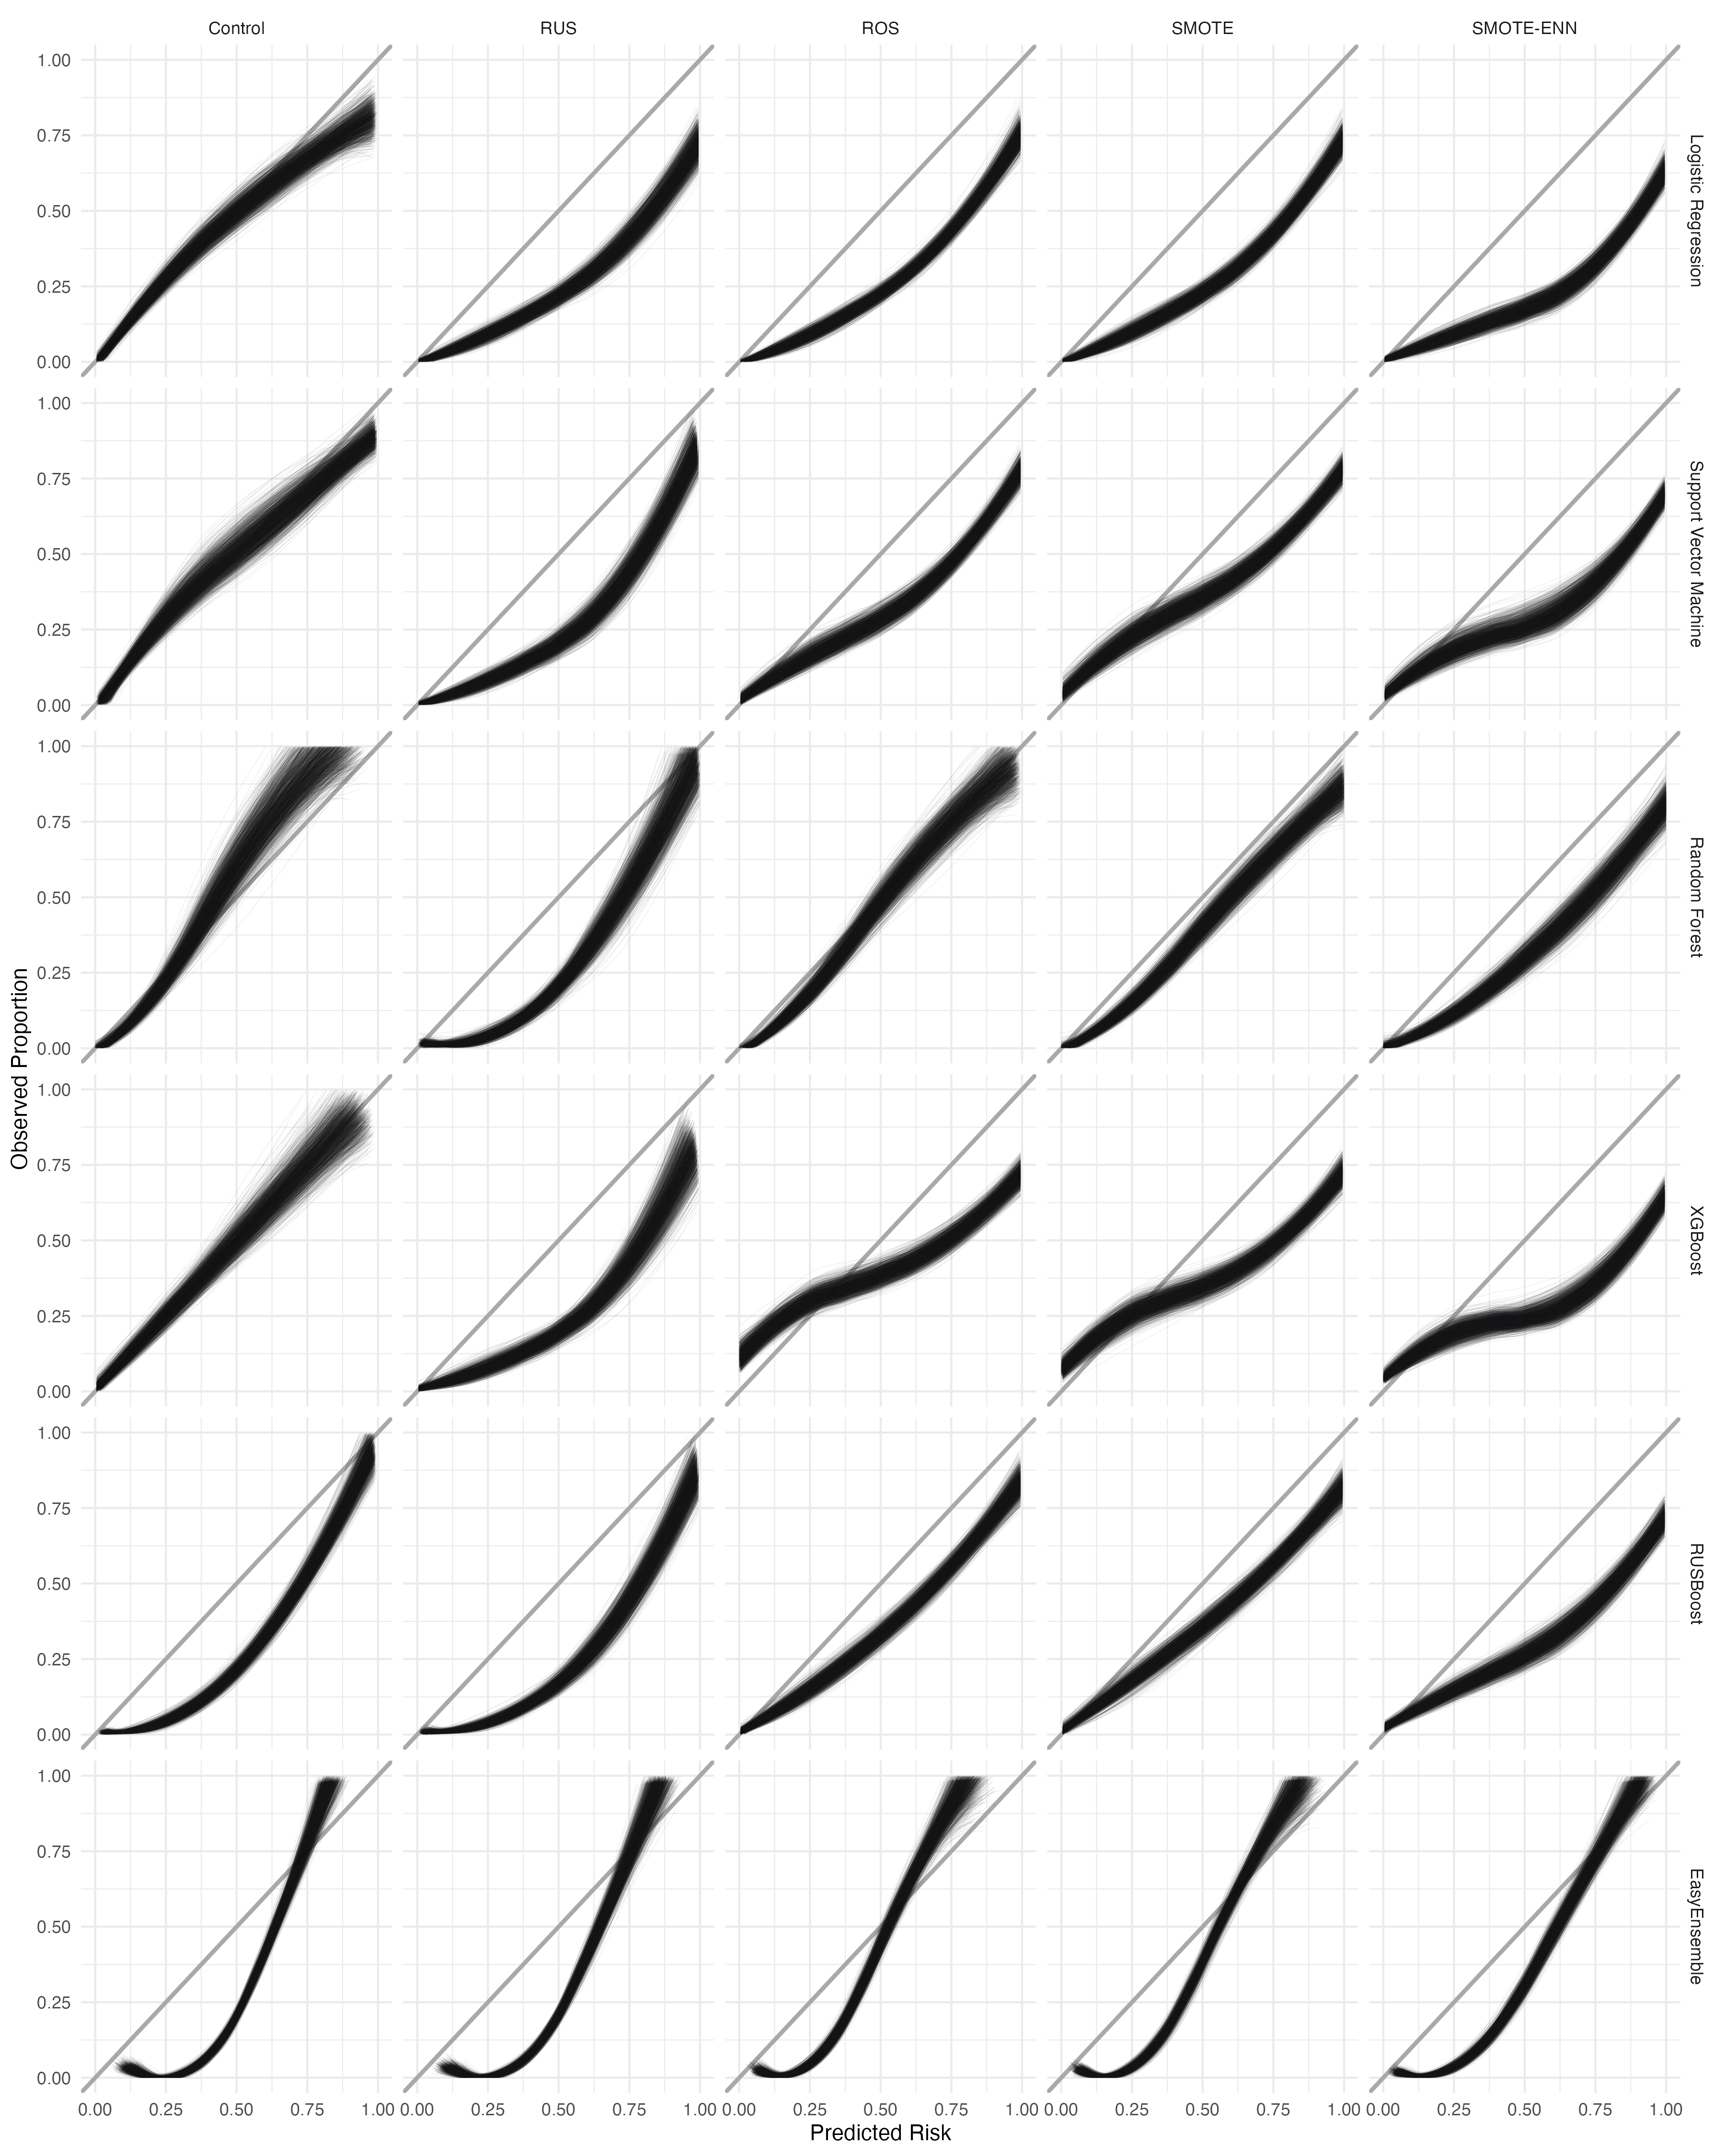
\includegraphics[width=0.7\linewidth]{./figures/calibration_plot_manuscript_sc17} 

}

\caption{Flexible calibration curves for each of 2000 simulation iterations in simulation scenario 17. This simulation scenario is characterized by 16 predictors, double the required sample size (2N) and moderately imbalanced data (event fraction = 0.2). Flexible curves were generated using raw predicted risks; no re-calibration. Imbalance corrections: RUS (random undersampling), ROS (random oversampling), SMOTE (synthetic majority oversampling), SENN (synthetic majority oversampling with Wilson's Edited Nearest Neighbors).\label{fig:cal_17}}\label{fig:unnamed-chunk-19}
\end{figure}
\clearpage
\begin{figure}

{\centering \includegraphics[width=0.7\linewidth]{./figures/calibration_plot_manuscript_sc18} 

}

\caption{Flexible calibration curves for each of 2000 simulation iterations in simulation scenario 18. This simulation scenario is characterized by 16 predictors, double the required sample size (2N) and strongly imbalanced data (event fraction = 0.02). Flexible curves were generated using raw predicted risks; no re-calibration. Imbalance corrections: RUS (random undersampling), ROS (random oversampling), SMOTE (synthetic majority oversampling), SENN (synthetic majority oversampling with Wilson's Edited Nearest Neighbors).\label{fig:cal_18}}\label{fig:unnamed-chunk-20}
\end{figure}

\newpage

\hypertarget{calibration-plots-after-re-calibration}{%
\subsubsection{\texorpdfstring{Calibration Plots (after
re-calibration)\\
}{Calibration Plots (after re-calibration) }}\label{calibration-plots-after-re-calibration}}

\hfill\break

\begin{figure}[h]

{\centering \includegraphics[width=0.7\linewidth]{./figures/calibration_plot_manuscript_sc1_recalibrated} 

}

\caption{Flexible calibration curves for each of 2000 simulation iterations in simulation scenario 1. This simulation scenario is characterized by 8 predictors, half the required sample size (0.5N) and class balanced data (event fraction = 0.5). Flexible curves were generated using re-calibrated predicted risks. Imbalance corrections: RUS (random undersampling), ROS (random oversampling), SMOTE (synthetic majority oversampling), SENN (synthetic majority oversampling with Wilson's Edited Nearest Neighbors).\label{fig:recal_1}}\label{fig:unnamed-chunk-21}
\end{figure}

\begin{figure}

{\centering \includegraphics[width=0.7\linewidth]{./figures/calibration_plot_manuscript_sc2_recalibrated} 

}

\caption{Flexible calibration curves for each of 2000 simulation iterations in simulation scenario 2. This simulation scenario is characterized by 8 predictors, half the required sample size (0.5N) and moderately imbalanced data (event fraction = 0.2). Flexible curves were generated using re-calibrated predicted risks. Imbalance corrections: RUS (random undersampling), ROS (random oversampling), SMOTE (synthetic majority oversampling), SENN (synthetic majority oversampling with Wilson's Edited Nearest Neighbors).\label{fig:recal_2}}\label{fig:unnamed-chunk-22}
\end{figure}

\begin{figure}

{\centering \includegraphics[width=0.7\linewidth]{./figures/calibration_plot_manuscript_sc3_recalibrated} 

}

\caption{Flexible calibration curves for each of 2000 simulation iterations in simulation scenario 3. This simulation scenario is characterized by 8 predictors, half the required sample size (0.5N) and strongly imbalanced data (event fraction = 0.02). Flexible curves were generated using re-calibrated predicted risks. Imbalance corrections: RUS (random undersampling), ROS (random oversampling), SMOTE (synthetic majority oversampling), SENN (synthetic majority oversampling with Wilson's Edited Nearest Neighbors).\label{fig:recal_3}}\label{fig:unnamed-chunk-23}
\end{figure}

\begin{figure}

{\centering 
\includegraphics[width=0.7\linewidth]{./figures/calibration_plot_manuscript_sc4_recalibrated} 

}

\caption{Flexible calibration curves for each of 2000 simulation iterations in simulation scenario 4. This simulation scenario is characterized by 8 predictors, minimum required sample size (N) and class balanced data (event fraction = 0.5). Flexible curves were generated using re-calibrated predicted risks. Imbalance corrections: RUS (random undersampling), ROS (random oversampling), SMOTE (synthetic majority oversampling), SENN (synthetic majority oversampling with Wilson's Edited Nearest Neighbors).\label{fig:recal_4}}\label{fig:unnamed-chunk-24}
\end{figure}

\begin{figure}

{\centering \includegraphics[width=0.7\linewidth]{./figures/calibration_plot_manuscript_sc5_recalibrated} 

}

\caption{Flexible calibration curves for each of 2000 simulation iterations in simulation scenario 5. This simulation scenario is characterized by 8 predictors, minimum required sample size (N) and moderately imbalanced data (event fraction = 0.2). Flexible curves were generated using re-calibrated predicted risks. Imbalance corrections: RUS (random undersampling), ROS (random oversampling), SMOTE (synthetic majority oversampling), SENN (synthetic majority oversampling with Wilson's Edited Nearest Neighbors). \label{fig:recal_5}}\label{fig:unnamed-chunk-25}
\end{figure}

\begin{figure}

{\centering \includegraphics[width=0.7\linewidth]{./figures/calibration_plot_manuscript_sc6_recalibrated} 

}

\caption{Flexible calibration curves for each of 2000 simulation iterations in simulation scenario 6. This simulation scenario is characterized by 8 predictors, minimum required sample size (N) and strongly imbalanced data (event fraction = 0.02). Flexible curves were generated using re-calibrated predicted risks. Imbalance corrections: RUS (random undersampling), ROS (random oversampling), SMOTE (synthetic majority oversampling), SENN (synthetic majority oversampling with Wilson's Edited Nearest Neighbors). \label{fig:recal_6}}\label{fig:unnamed-chunk-26}
\end{figure}

\begin{figure}

{\centering 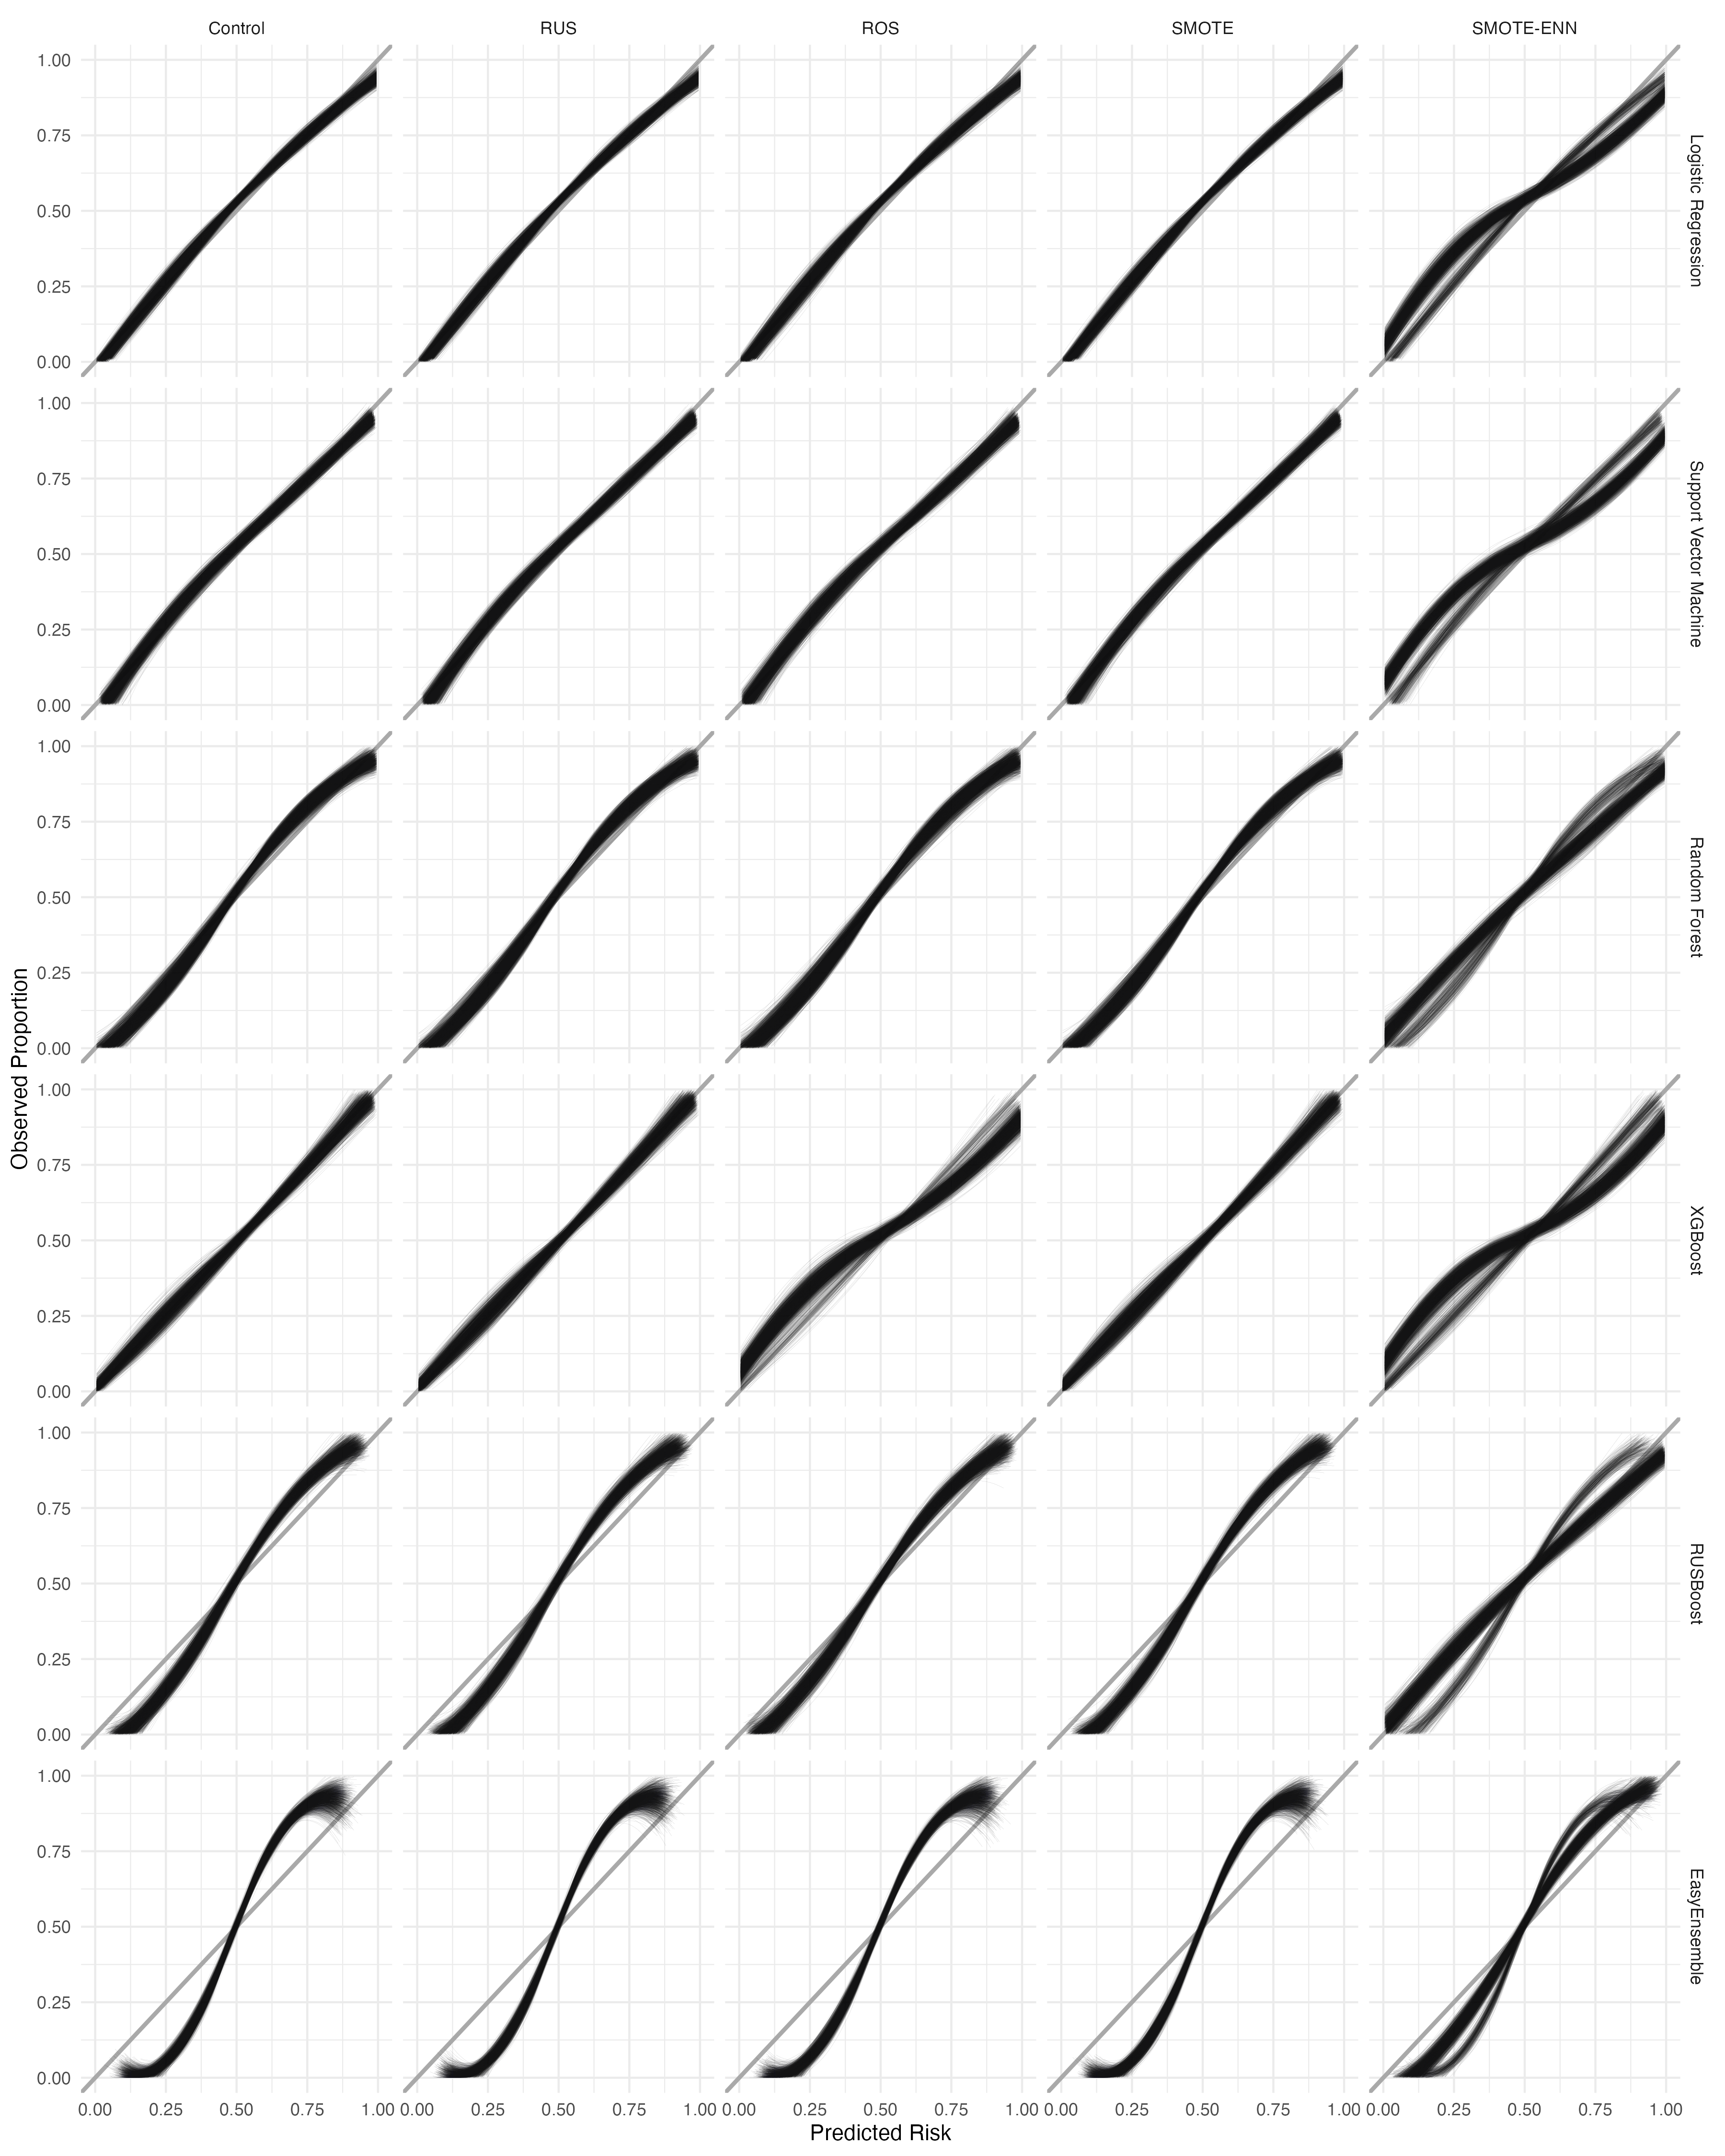
\includegraphics[width=0.7\linewidth]{./figures/calibration_plot_manuscript_sc7_recalibrated} 

}

\caption{Flexible calibration curves for each of 2000 simulation iterations in simulation scenario 7. This simulation scenario is characterized by 8 predictors, double the required sample size (2N) and class balanced data (event fraction = 0.5). Flexible curves were generated using re-calibrated predicted risks. Imbalance corrections: RUS (random undersampling), ROS (random oversampling), SMOTE (synthetic majority oversampling), SENN (synthetic majority oversampling with Wilson's Edited Nearest Neighbors). \label{fig:recal_7}}\label{fig:unnamed-chunk-27}
\end{figure}

\begin{figure}

{\centering \includegraphics[width=0.7\linewidth]{./figures/calibration_plot_manuscript_sc8_recalibrated} 

}

\caption{Flexible calibration curves for each of 2000 simulation iterations in simulation scenario 8. This simulation scenario is characterized by 8 predictors, double the required sample size (2N) and moderately imbalanced data (event fraction = 0.2). Flexible curves were generated using re-calibrated predicted risks. Imbalance corrections: RUS (random undersampling), ROS (random oversampling), SMOTE (synthetic majority oversampling), SENN (synthetic majority oversampling with Wilson's Edited Nearest Neighbors). \label{fig:recal_8}}\label{fig:unnamed-chunk-28}
\end{figure}

\begin{figure}

{\centering \includegraphics[width=0.7\linewidth]{./figures/calibration_plot_manuscript_sc9_recalibrated} 

}

\caption{Flexible calibration curves for each of 2000 simulation iterations in simulation scenario 9. This simulation scenario is characterized by 8 predictors, double the required sample size (2N) and strongly imbalanced data (event fraction = 0.02). Flexible curves were generated using re-calibrated predicted risks. Imbalance corrections: RUS (random undersampling), ROS (random oversampling), SMOTE (synthetic majority oversampling), SENN (synthetic majority oversampling with Wilson's Edited Nearest Neighbors). \label{fig:recal_9}}\label{fig:unnamed-chunk-29}
\end{figure}

\begin{figure}

{\centering \includegraphics[width=0.7\linewidth]{./figures/calibration_plot_manuscript_sc10_recalibrated} 

}

\caption{Flexible calibration curves for each of 2000 simulation iterations in simulation scenario 10. This simulation scenario is characterized by 16 predictors, half the required sample size (0.5N) and class balanced data (event fraction = 0.5). Flexible curves were generated using re-calibrated predicted risks. Imbalance corrections: RUS (random undersampling), ROS (random oversampling), SMOTE (synthetic majority oversampling), SENN (synthetic majority oversampling with Wilson's Edited Nearest Neighbors). \label{fig:recal_10}}\label{fig:unnamed-chunk-30}
\end{figure}

\begin{figure}

{\centering \includegraphics[width=0.7\linewidth]{./figures/calibration_plot_manuscript_sc11_recalibrated} 

}

\caption{Flexible calibration curves for each of 2000 simulation iterations in simulation scenario 11. This simulation scenario is characterized by 16 predictors, half the required sample size (0.5N) and moderately imbalanced data (event fraction = 0.2). Flexible curves were generated using re-calibrated predicted risks. Imbalance corrections: RUS (random undersampling), ROS (random oversampling), SMOTE (synthetic majority oversampling), SENN (synthetic majority oversampling with Wilson's Edited Nearest Neighbors). \label{fig:recal_11}}\label{fig:unnamed-chunk-31}
\end{figure}

\begin{figure}

{\centering \includegraphics[width=0.7\linewidth]{./figures/calibration_plot_manuscript_sc12_recalibrated} 

}

\caption{Flexible calibration curves for each of 2000 simulation iterations in simulation scenario 12. This simulation scenario is characterized by 16 predictors, half the required sample size (0.5N) and strongly imbalanced data (event fraction = 0.02). Flexible curves were generated using re-calibrated predicted risks. Imbalance corrections: RUS (random undersampling), ROS (random oversampling), SMOTE (synthetic majority oversampling), SENN (synthetic majority oversampling with Wilson's Edited Nearest Neighbors). \label{fig:recal_12}}\label{fig:unnamed-chunk-32}
\end{figure}

\begin{figure}

{\centering 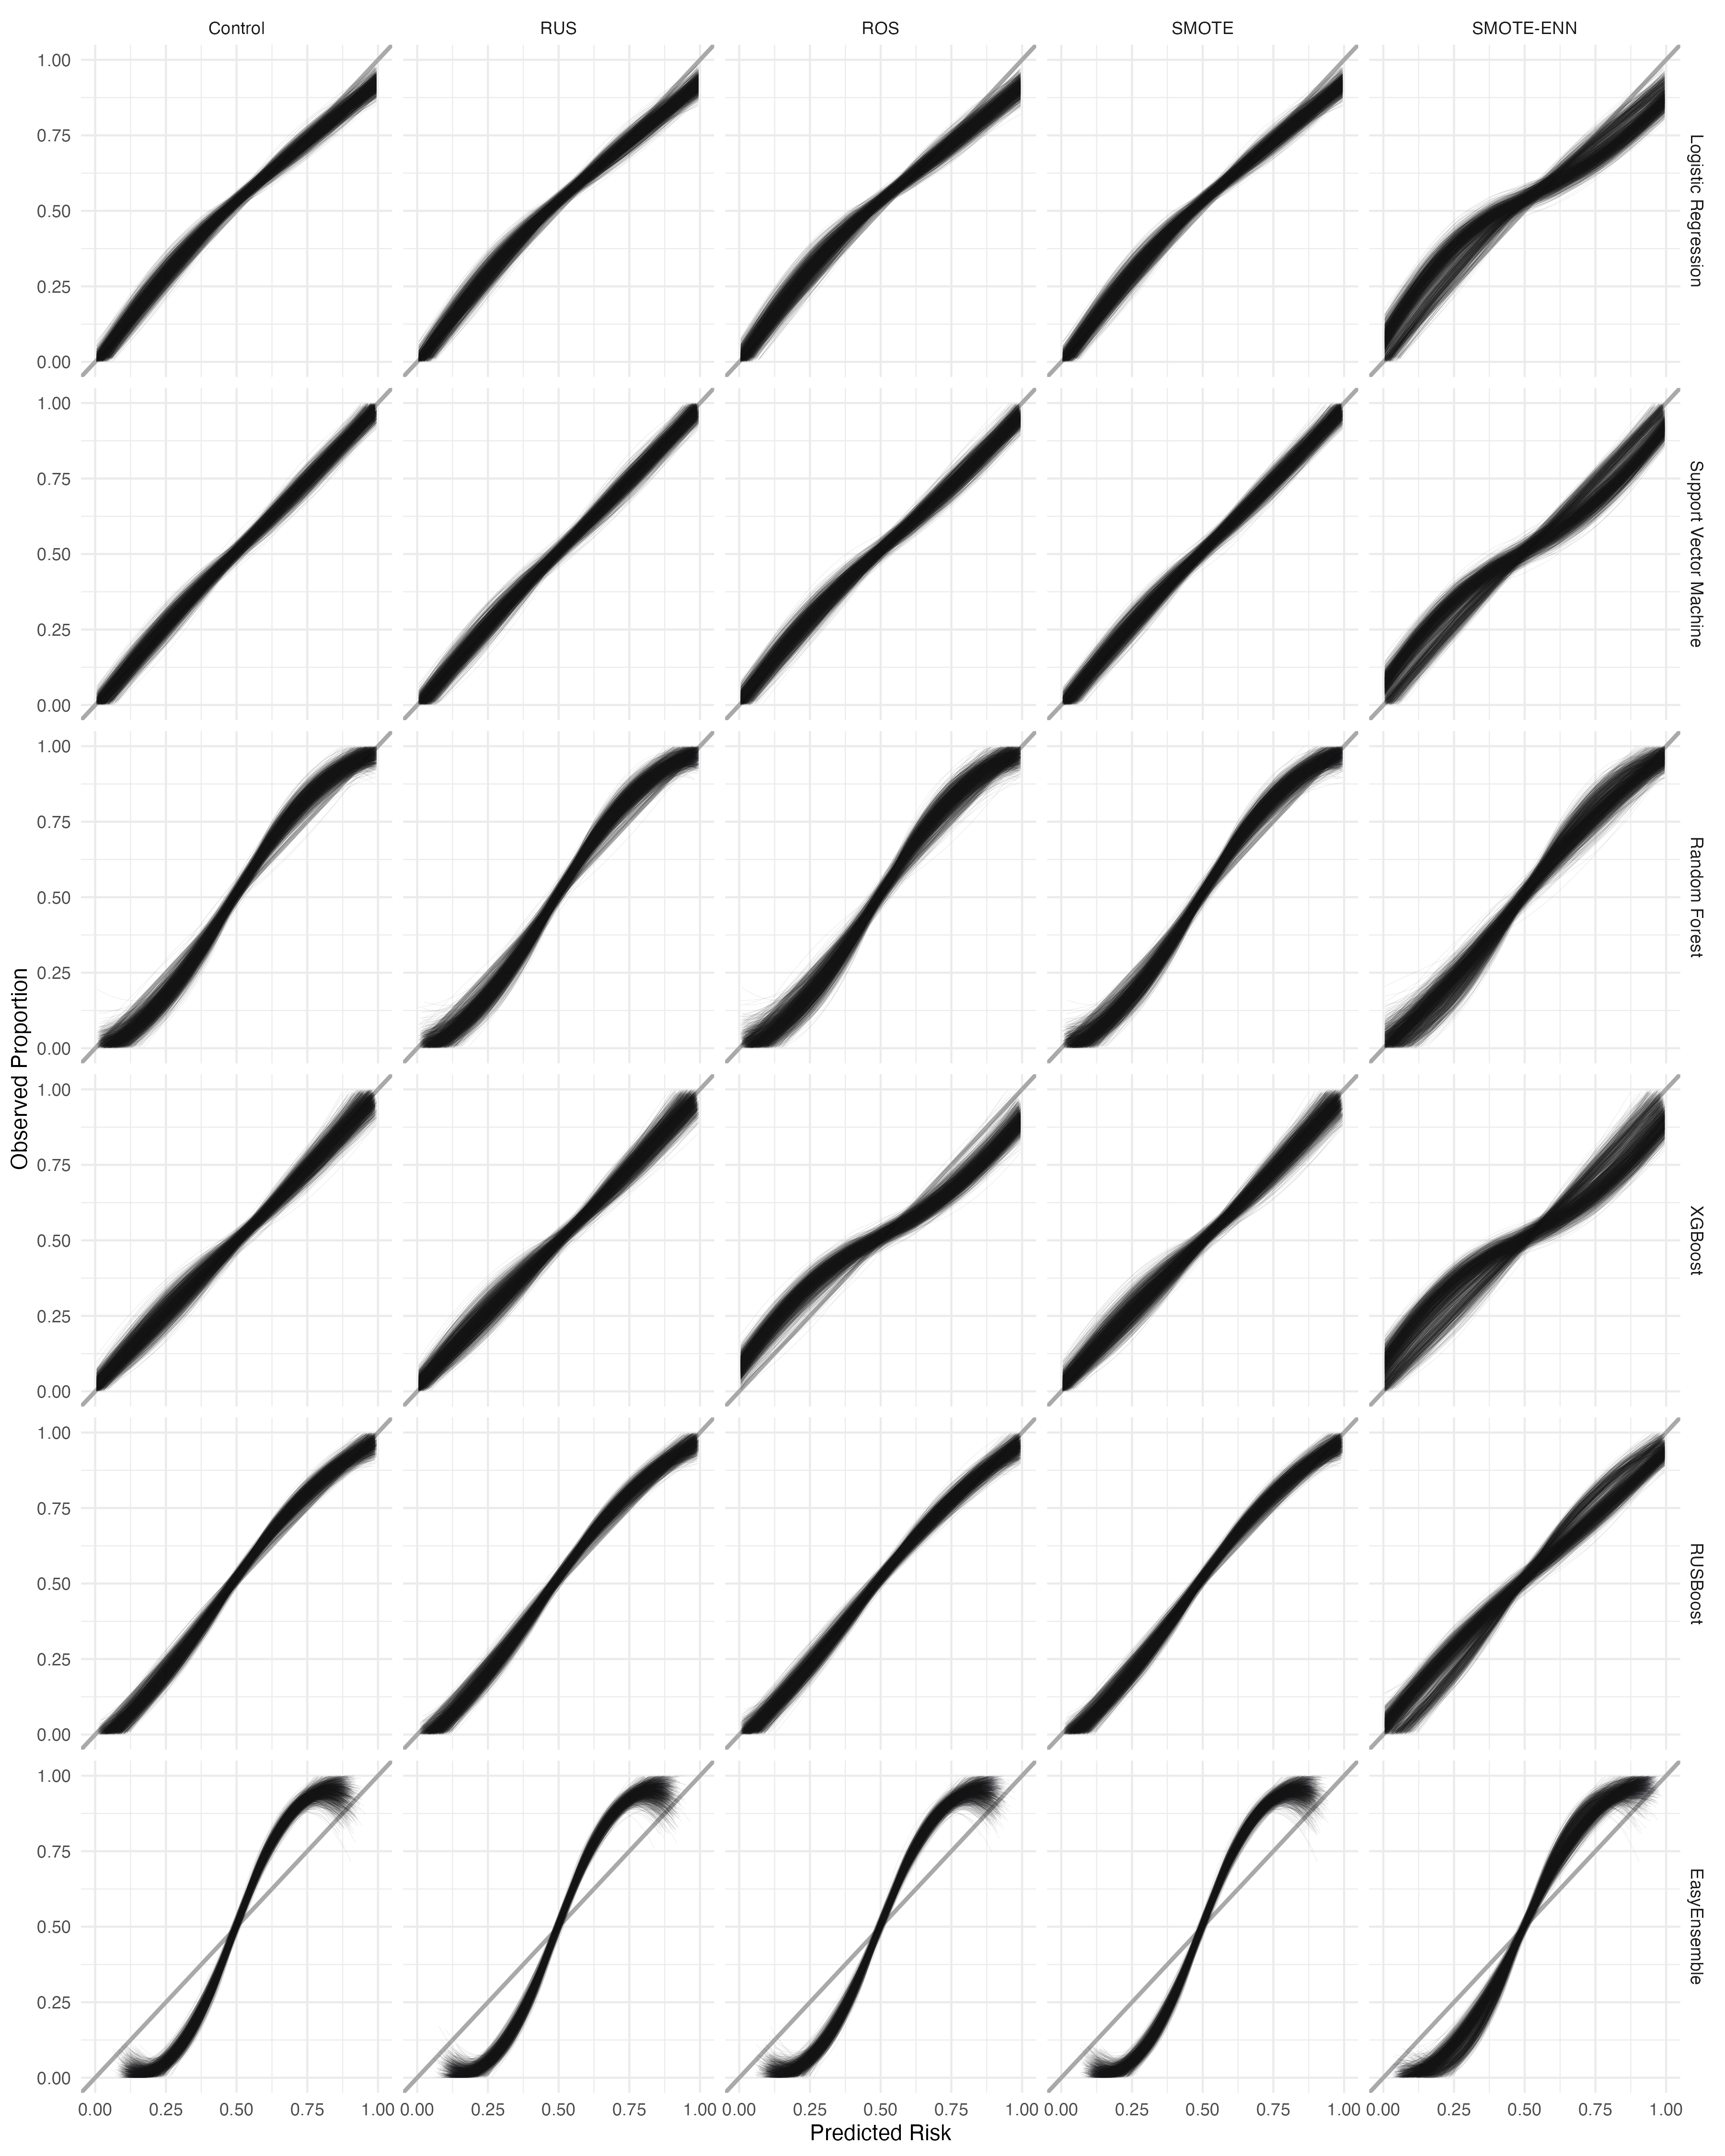
\includegraphics[width=0.7\linewidth]{./figures/calibration_plot_manuscript_sc13_recalibrated} 

}

\caption{Flexible calibration curves for each of 2000 simulation iterations in simulation scenario 13. This simulation scenario is characterized by 16 predictors, minimum required sample size (N) and class balanced data (event fraction = 0.5). Flexible curves were generated using re-calibrated predicted risks. Imbalance corrections: RUS (random undersampling), ROS (random oversampling), SMOTE (synthetic majority oversampling), SENN (synthetic majority oversampling with Wilson's Edited Nearest Neighbors). \label{fig:recal_13}}\label{fig:unnamed-chunk-33}
\end{figure}

\begin{figure}

{\centering \includegraphics[width=0.7\linewidth]{./figures/calibration_plot_manuscript_sc14_recalibrated} 

}

\caption{Flexible calibration curves for each of 2000 simulation iterations in simulation scenario 14. This simulation scenario is characterized by 16 predictors, minimum required sample size (N) and moderately imbalanced data (event fraction = 0.2). Flexible curves were generated using re-calibrated predicted risks. Imbalance corrections: RUS (random undersampling), ROS (random oversampling), SMOTE (synthetic majority oversampling), SENN (synthetic majority oversampling with Wilson's Edited Nearest Neighbors). \label{fig:recal_14}}\label{fig:unnamed-chunk-34}
\end{figure}

\begin{figure}

{\centering \includegraphics[width=0.7\linewidth]{./figures/calibration_plot_manuscript_sc15_recalibrated} 

}

\caption{Flexible calibration curves for each of 2000 simulation iterations in simulation scenario 15. This simulation scenario is characterized by 16 predictors, minimum required sample size (N) and strongly imbalanced data (event fraction = 0.02). Flexible curves were generated using re-calibrated predicted risks. Imbalance corrections: RUS (random undersampling), ROS (random oversampling), SMOTE (synthetic majority oversampling), SENN (synthetic majority oversampling with Wilson's Edited Nearest Neighbors). \label{fig:recal_15}}\label{fig:unnamed-chunk-35}
\end{figure}

\begin{figure}

{\centering 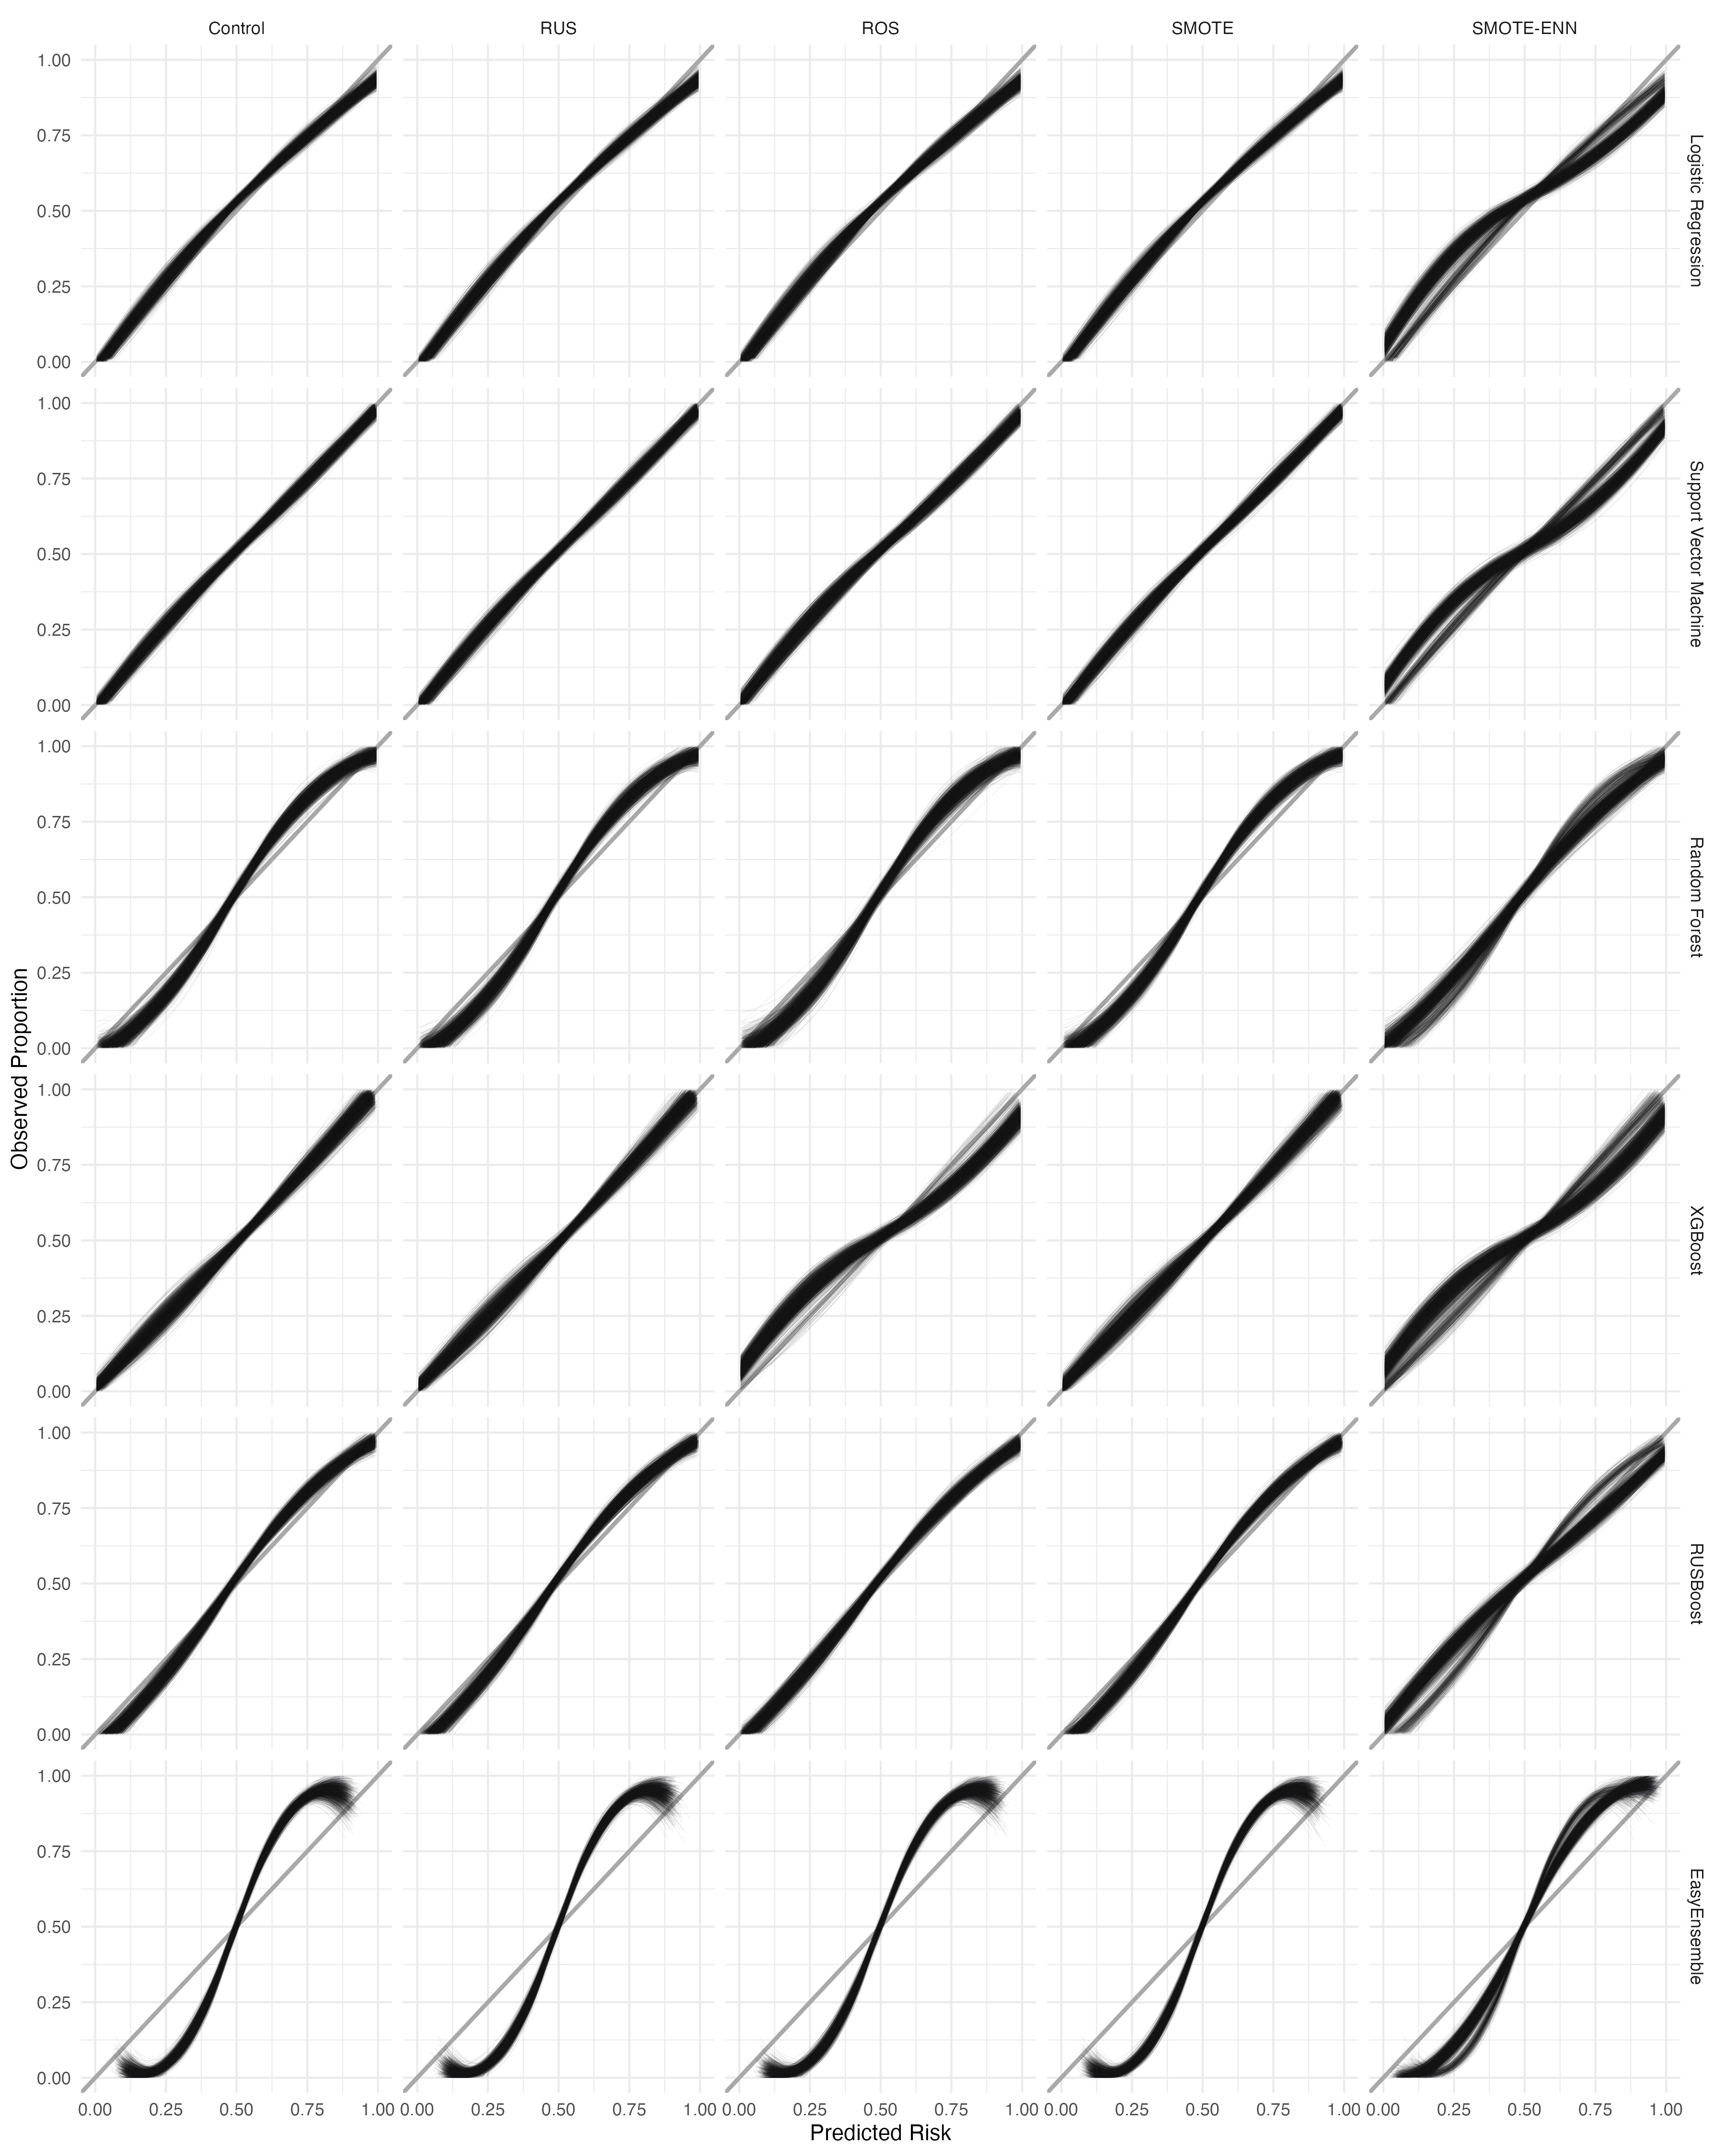
\includegraphics[width=0.7\linewidth]{./figures/calibration_plot_manuscript_sc16_recalibrated} 

}

\caption{Flexible calibration curves for each of 2000 simulation iterations in simulation scenario 16. This simulation scenario is characterized by 16 predictors, double the required sample size (2N) and class balanced data (event fraction = 0.5). Flexible curves were generated using re-calibrated predicted risks. Imbalance corrections: RUS (random undersampling), ROS (random oversampling), SMOTE (synthetic majority oversampling), SENN (synthetic majority oversampling with Wilson's Edited Nearest Neighbors). \label{fig:recal_16}}\label{fig:unnamed-chunk-36}
\end{figure}

\begin{figure}

{\centering 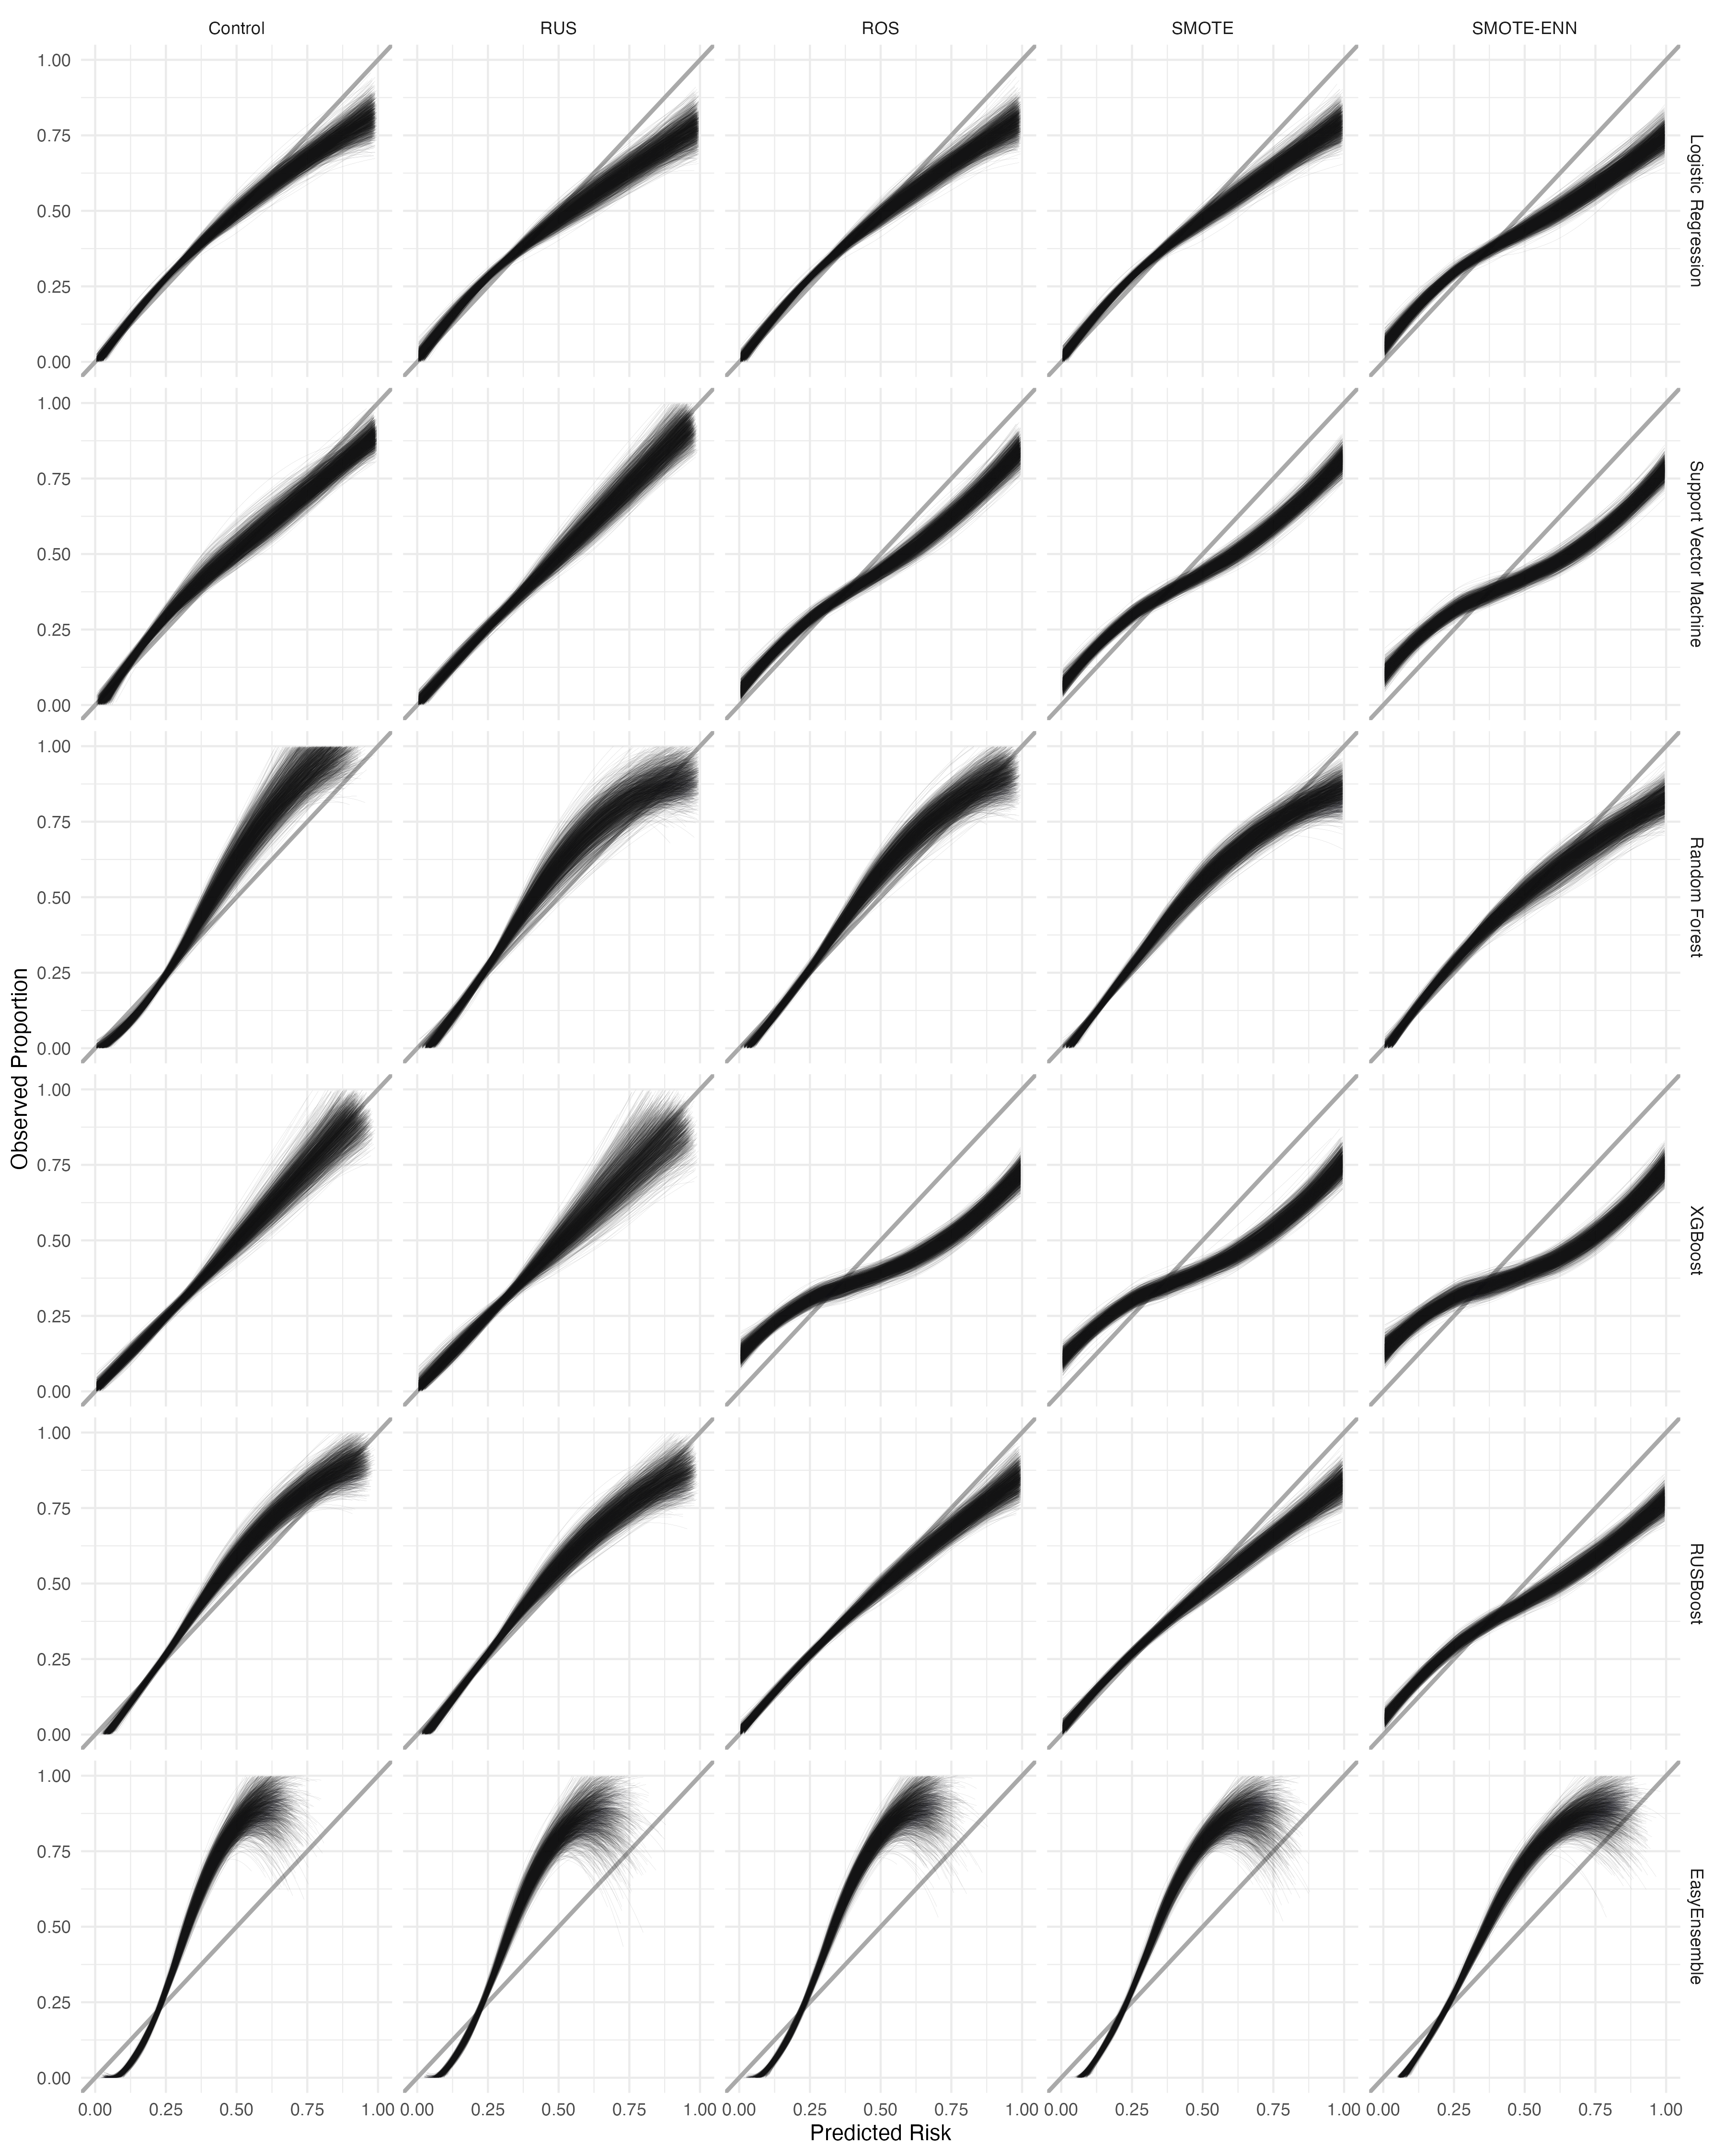
\includegraphics[width=0.7\linewidth]{./figures/calibration_plot_manuscript_sc17_recalibrated} 

}

\caption{Flexible calibration curves for each of 2000 simulation iterations in simulation scenario 17. This simulation scenario is characterized by 16 predictors, double the required sample size (2N) and moderately imbalanced data (event fraction = 0.2). Flexible curves were generated using re-calibrated predicted risks. Imbalance corrections: RUS (random undersampling), ROS (random oversampling), SMOTE (synthetic majority oversampling), SENN (synthetic majority oversampling with Wilson's Edited Nearest Neighbors). \label{fig:recal_17}}\label{fig:unnamed-chunk-37}
\end{figure}
\clearpage
\begin{figure}

{\centering \includegraphics[width=0.7\linewidth]{./figures/calibration_plot_manuscript_sc18_recalibrated} 

}

\caption{Flexible calibration curves for each of 2000 simulation iterations in simulation scenario 18. This simulation scenario is characterized by 16 predictors, double the required sample size (2N) and strongly imbalanced data (event fraction = 0.02). Flexible curves were generated using re-calibrated predicted risks. Imbalance corrections: RUS (random undersampling), ROS (random oversampling), SMOTE (synthetic majority oversampling), SENN (synthetic majority oversampling with Wilson's Edited Nearest Neighbors). \label{fig:recal_18}}\label{fig:unnamed-chunk-38}
\end{figure}

\newpage

\hypertarget{violin-plots-no-re-calibration}{%
\subsubsection{\texorpdfstring{Violin Plots (no re-calibration)\\
}{Violin Plots (no re-calibration) }}\label{violin-plots-no-re-calibration}}

\hfill\break

\begin{figure}[h]

{\centering 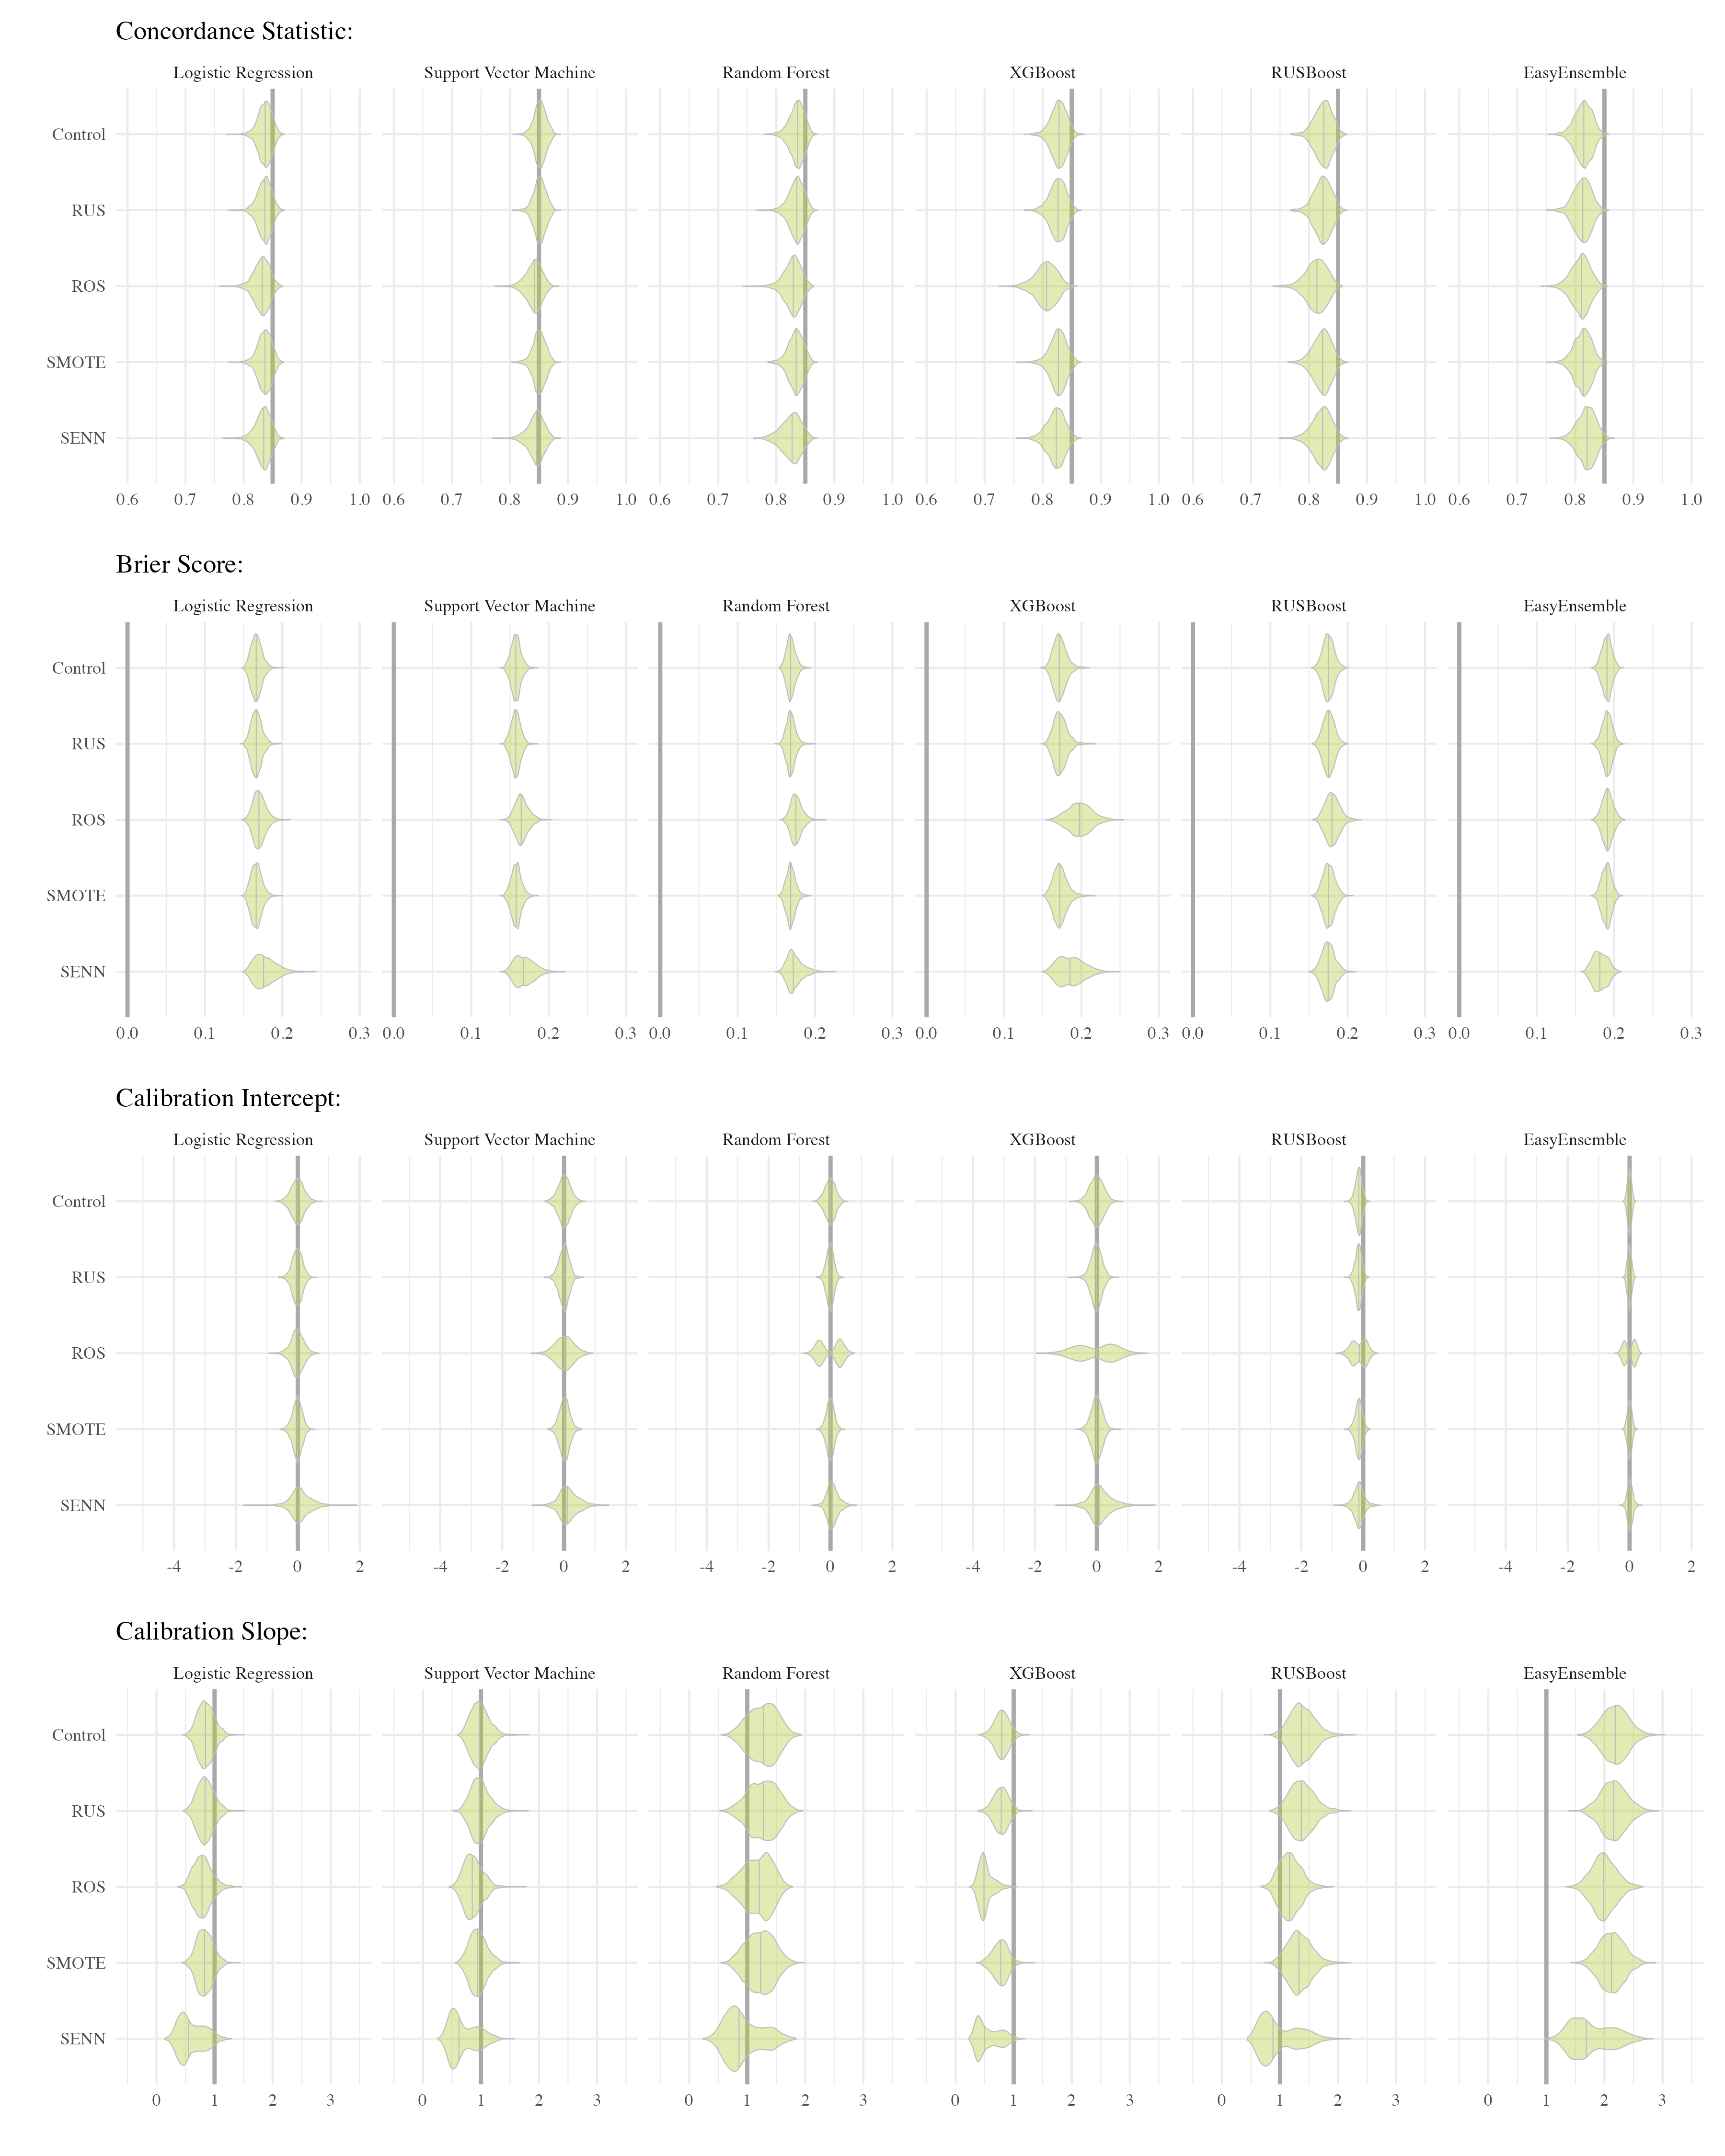
\includegraphics[width=0.7\linewidth]{./figures/performance_metrics_manuscript_sc1} 

}

\caption{Empirical performance metrics for each of 2000 simulation iterations in simulation scenario 1.  This simulation scenario is characterized by 8 predictors, half the required sample size (0.5N) and class balanced data (event fraction = 0.5). Empirical performance metrics were computed with raw predicted risks; no re-calibration. The target value highlighted for concordance statistic reflects the data-generating concordance statstic, 0.85.  Imbalance corrections: RUS (random undersampling), ROS (random oversampling), SMOTE (synthetic majority oversampling), SENN (synthetic majority oversampling with Wilson's Edited Nearest Neighbors). \label{fig:violin_1}}\label{fig:unnamed-chunk-39}
\end{figure}

\begin{figure}

{\centering 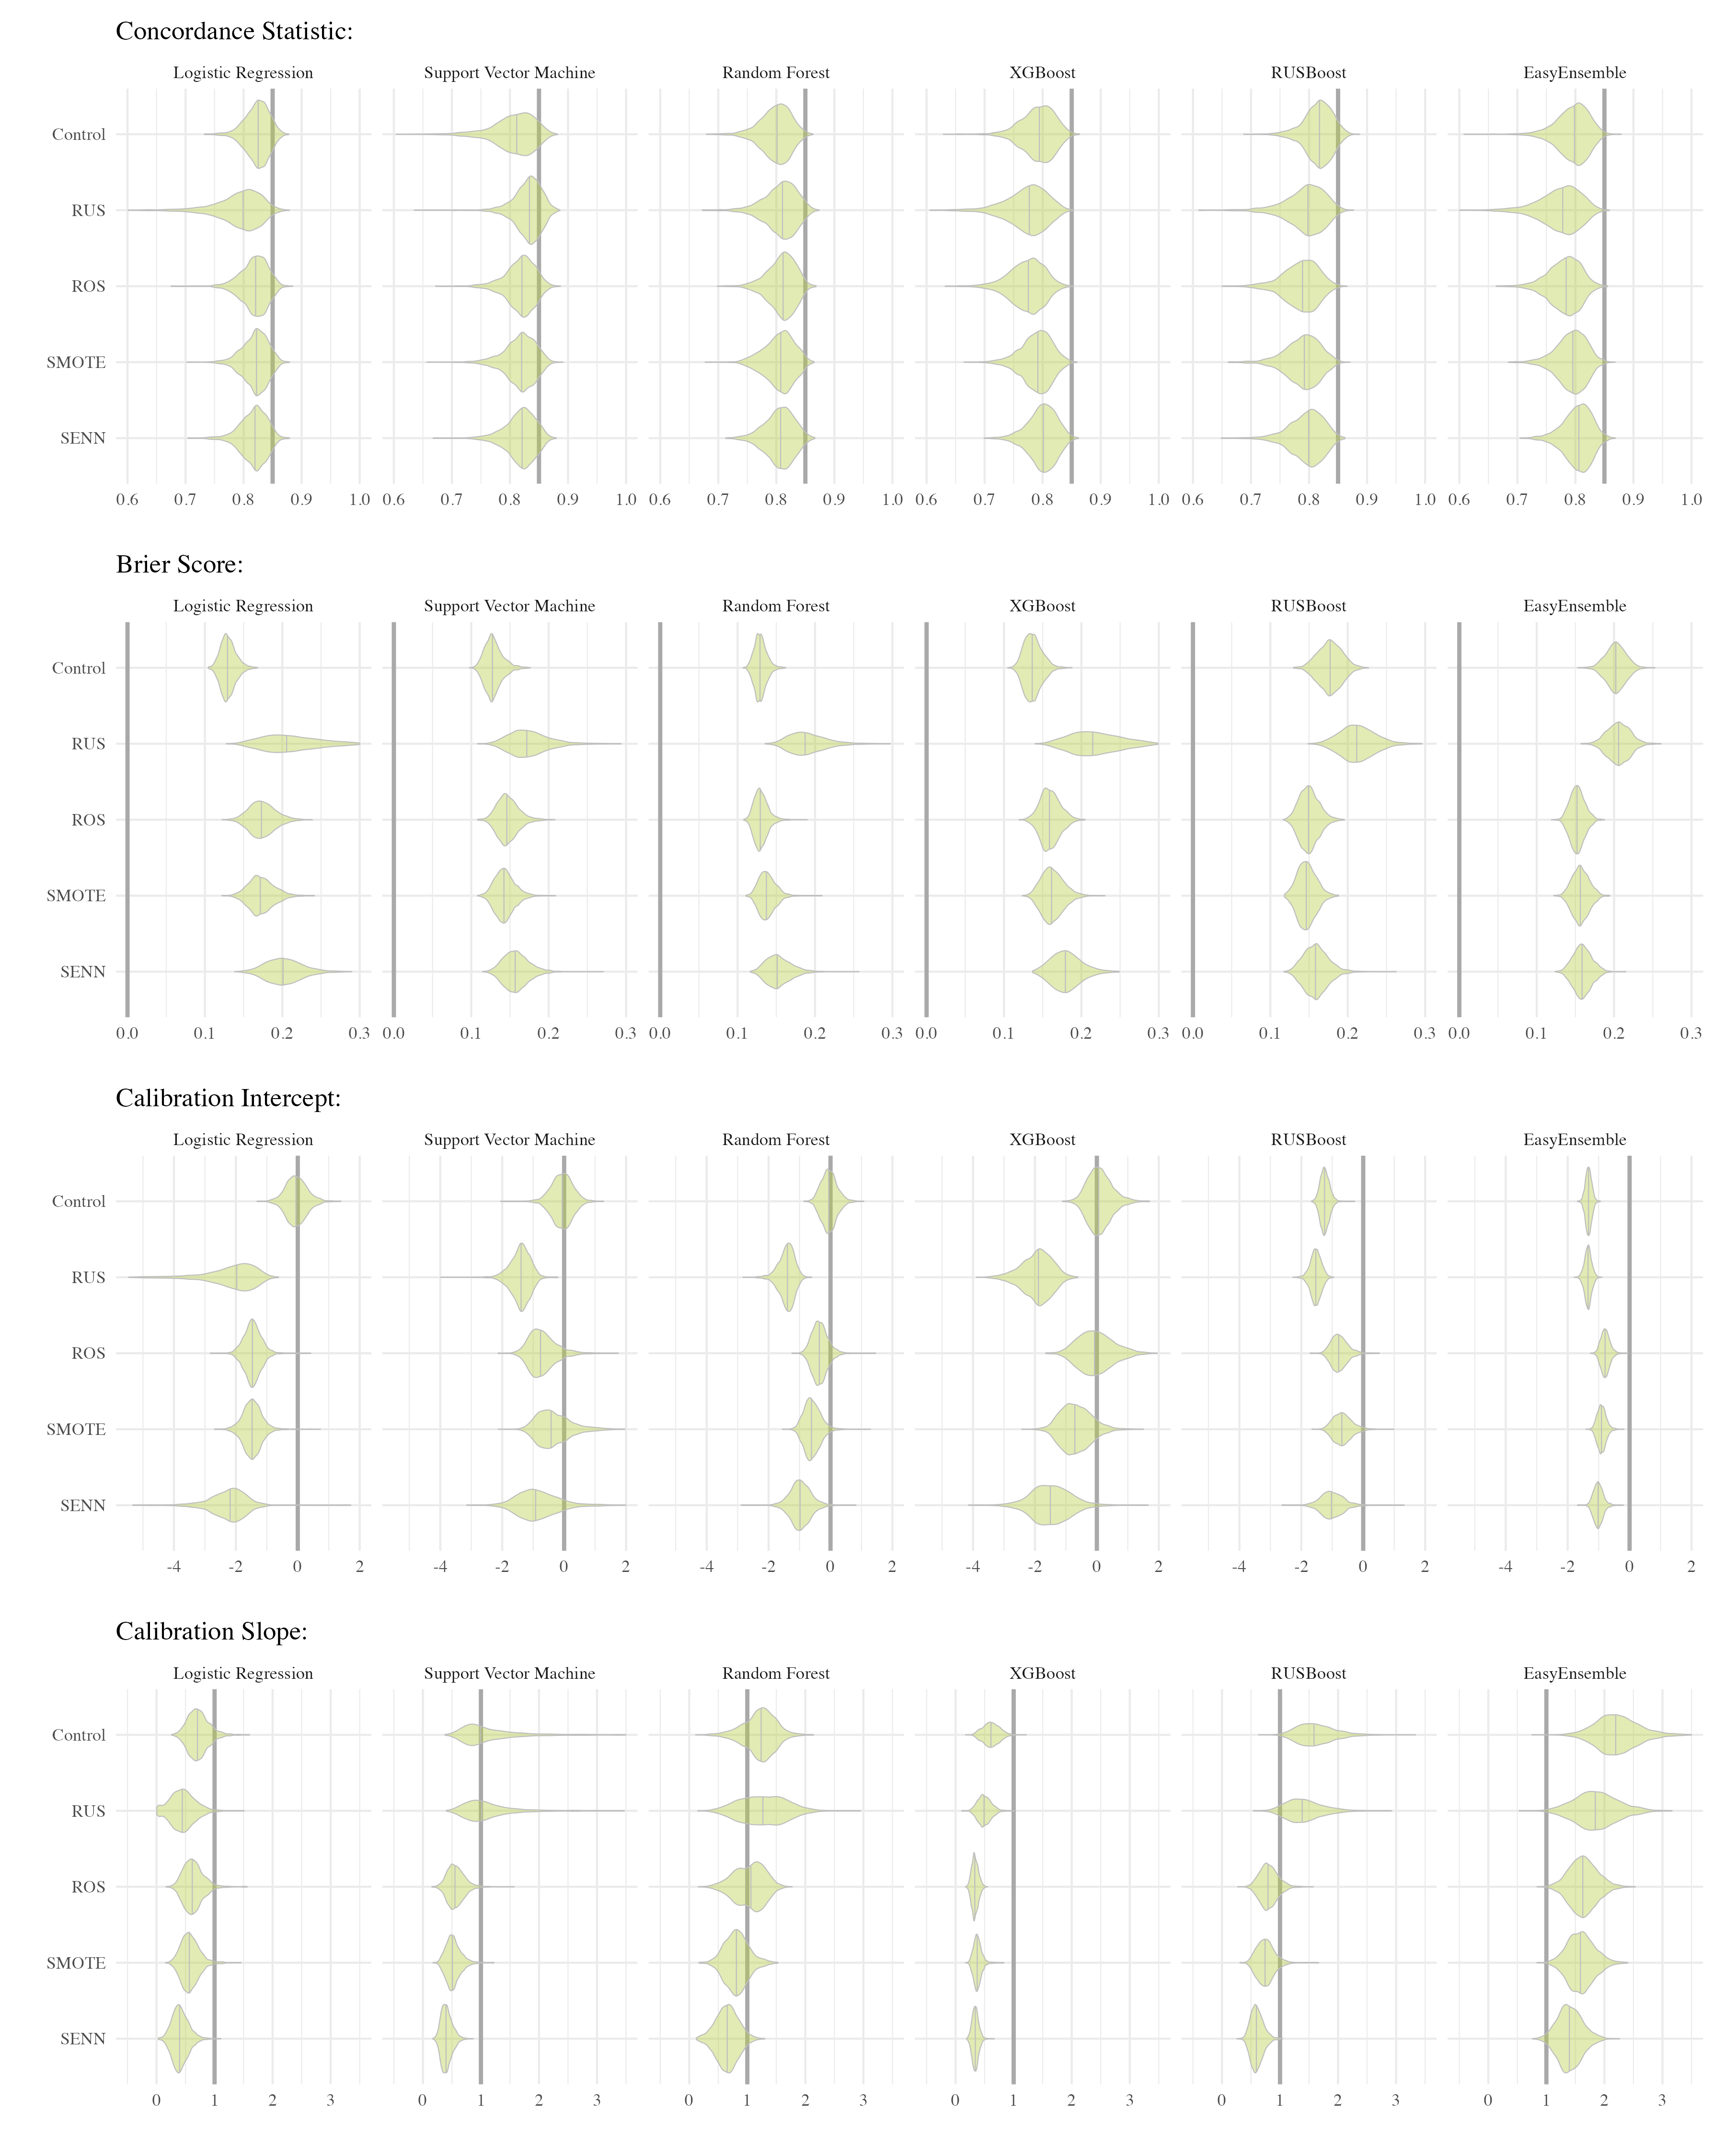
\includegraphics[width=0.7\linewidth]{./figures/performance_metrics_manuscript_sc2} 

}

\caption{Empirical performance metrics for each of 2000 simulation iterations in simulation scenario 2.  This simulation scenario is characterized by 8 predictors, half the required sample size (0.5N) and moderately imbalanced data (event fraction = 0.2). Empirical performance metrics were computed with raw predicted risks; no re-calibration. The target value highlighted for concordance statistic reflects the data-generating concordance statstic, 0.85. Imbalance corrections: RUS (random undersampling), ROS (random oversampling), SMOTE (synthetic majority oversampling), SENN (synthetic majority oversampling with Wilson's Edited Nearest Neighbors). \label{fig:violin_2}}\label{fig:unnamed-chunk-40}
\end{figure}

\begin{figure}

{\centering 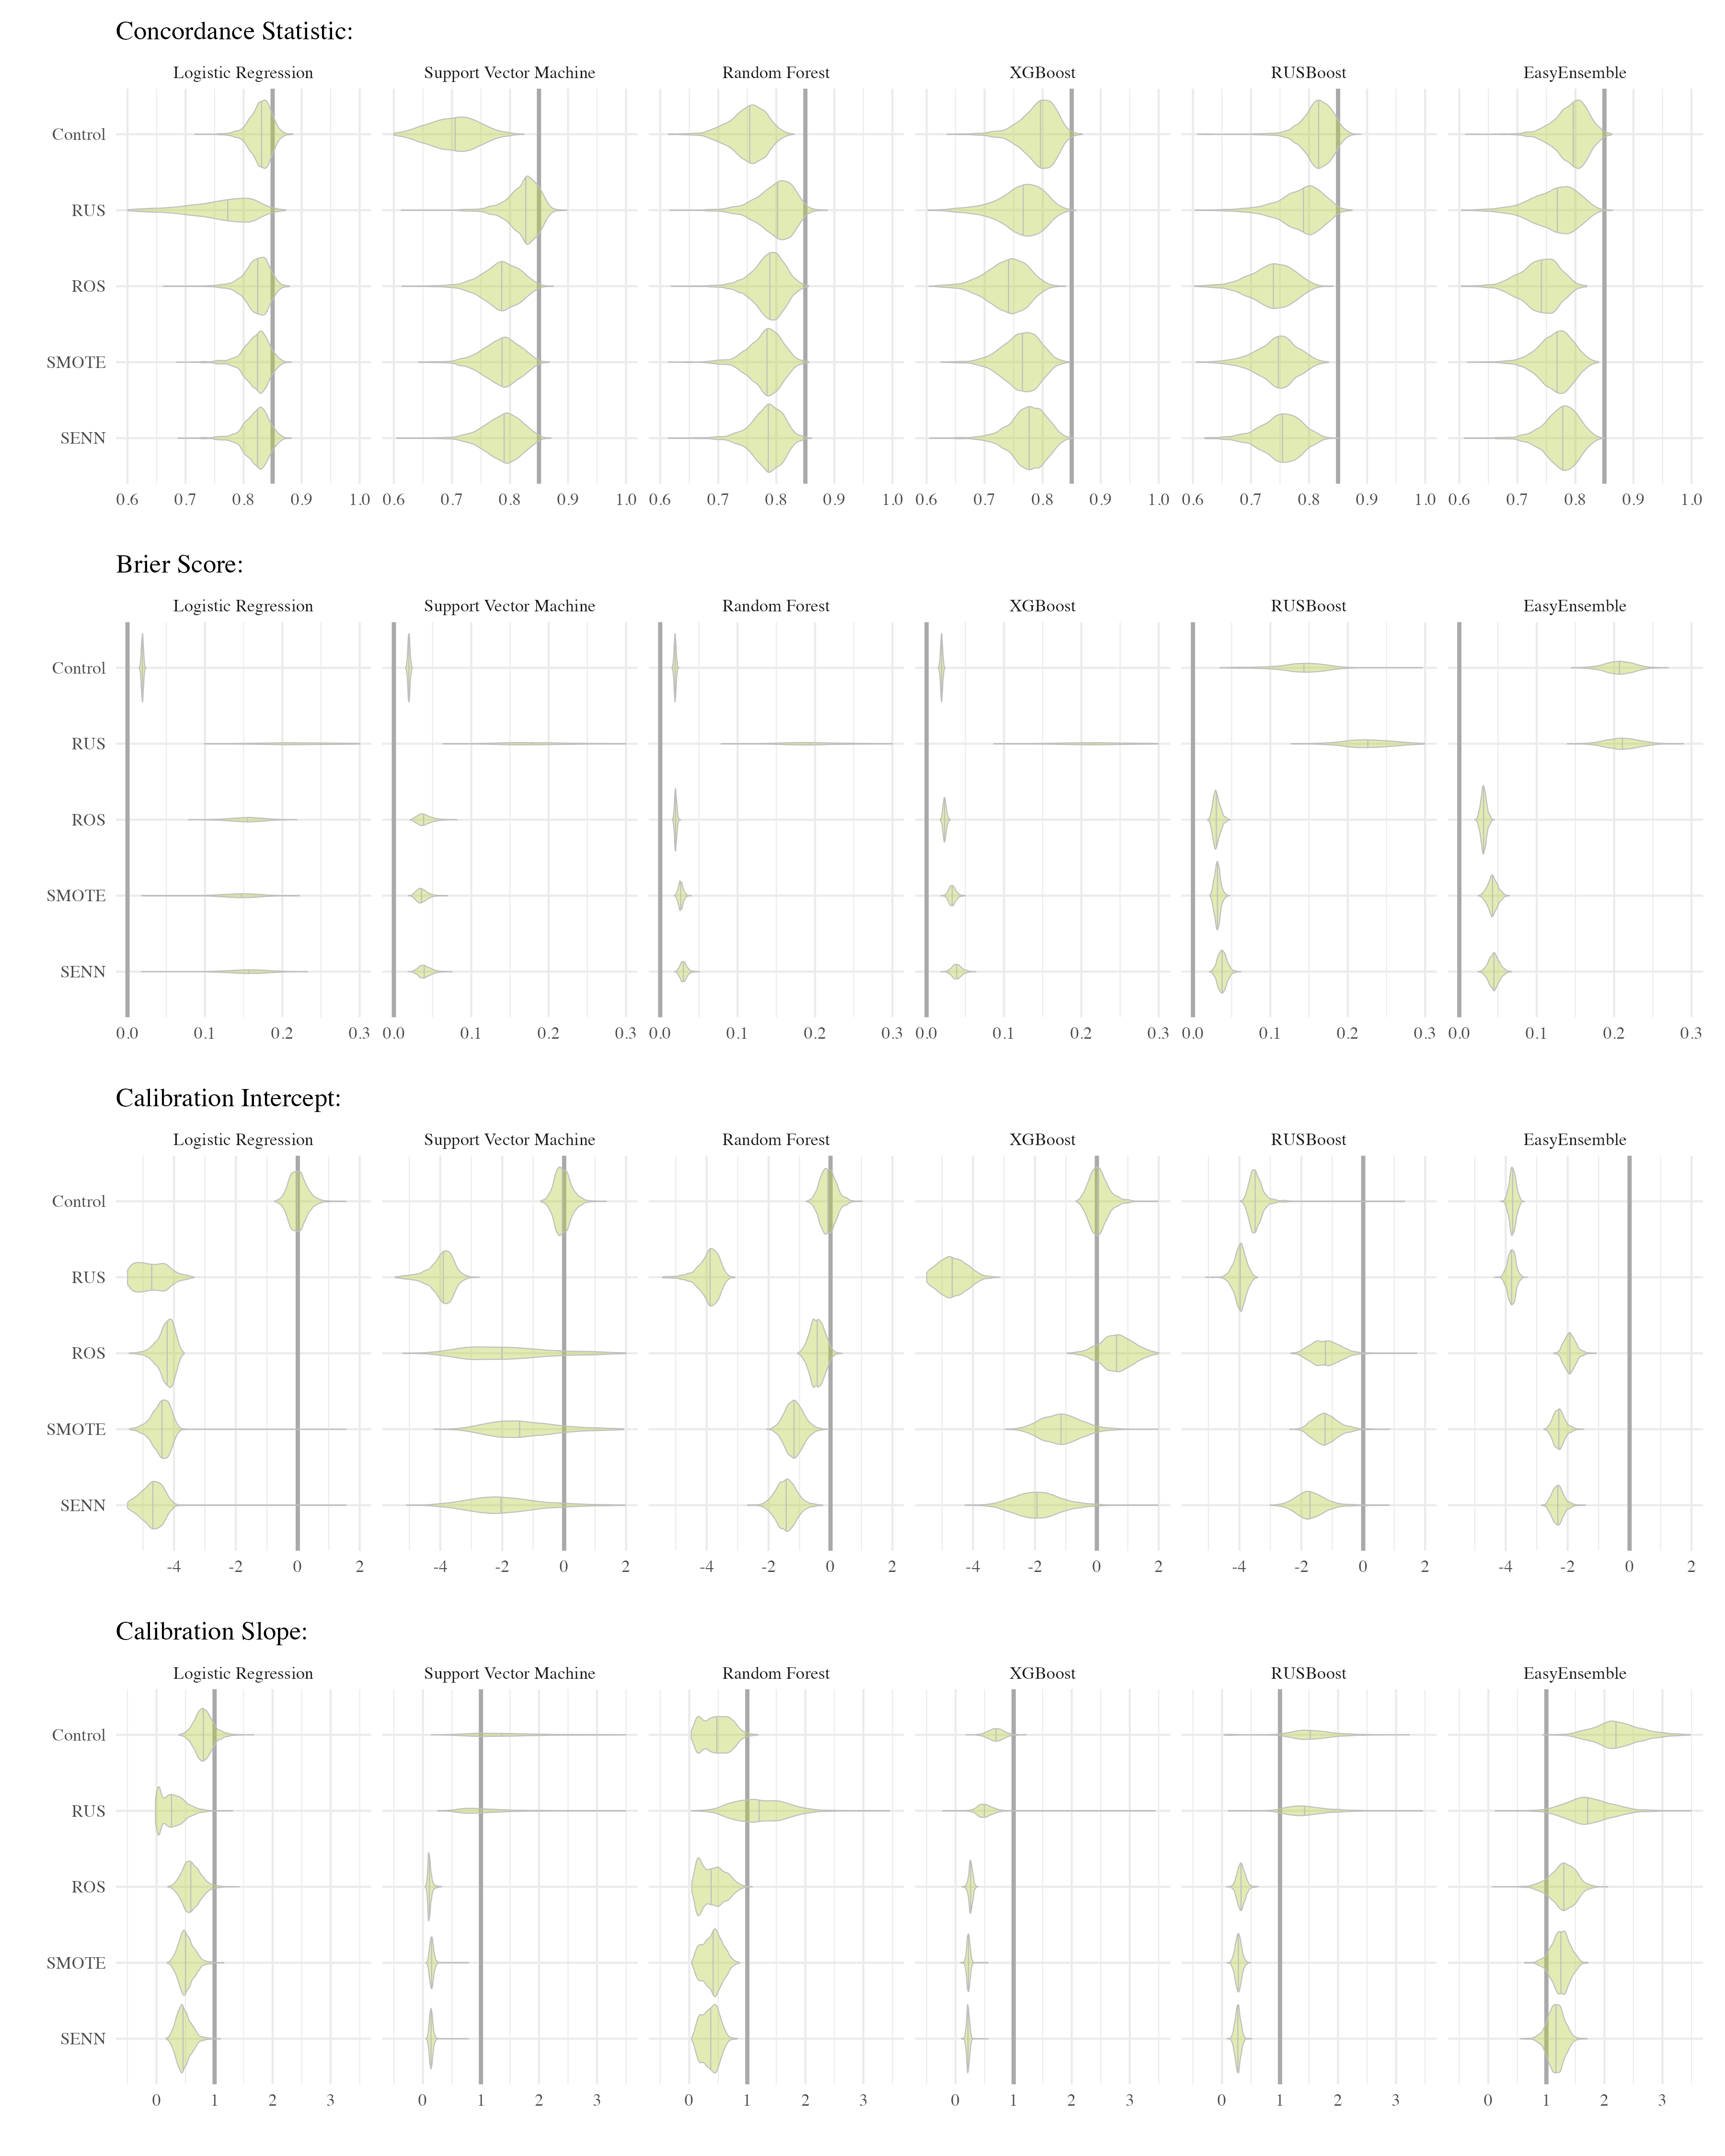
\includegraphics[width=0.7\linewidth]{./figures/performance_metrics_manuscript_sc3} 

}

\caption{Empirical performance metrics for each of 2000 simulation iterations in simulation scenario 3.  This simulation scenario is characterized by 8 predictors, half the required sample size (0.5N) and strongly imbalanced data (event fraction = 0.02). Empirical performance metrics were computed with raw predicted risks; no re-calibration. The target value highlighted for concordance statistic reflects the data-generating concordance statstic, 0.85. Imbalance corrections: RUS (random undersampling), ROS (random oversampling), SMOTE (synthetic majority oversampling), SENN (synthetic majority oversampling with Wilson's Edited Nearest Neighbors). \label{fig:violin_3}}\label{fig:unnamed-chunk-41}
\end{figure}

\begin{figure}

{\centering 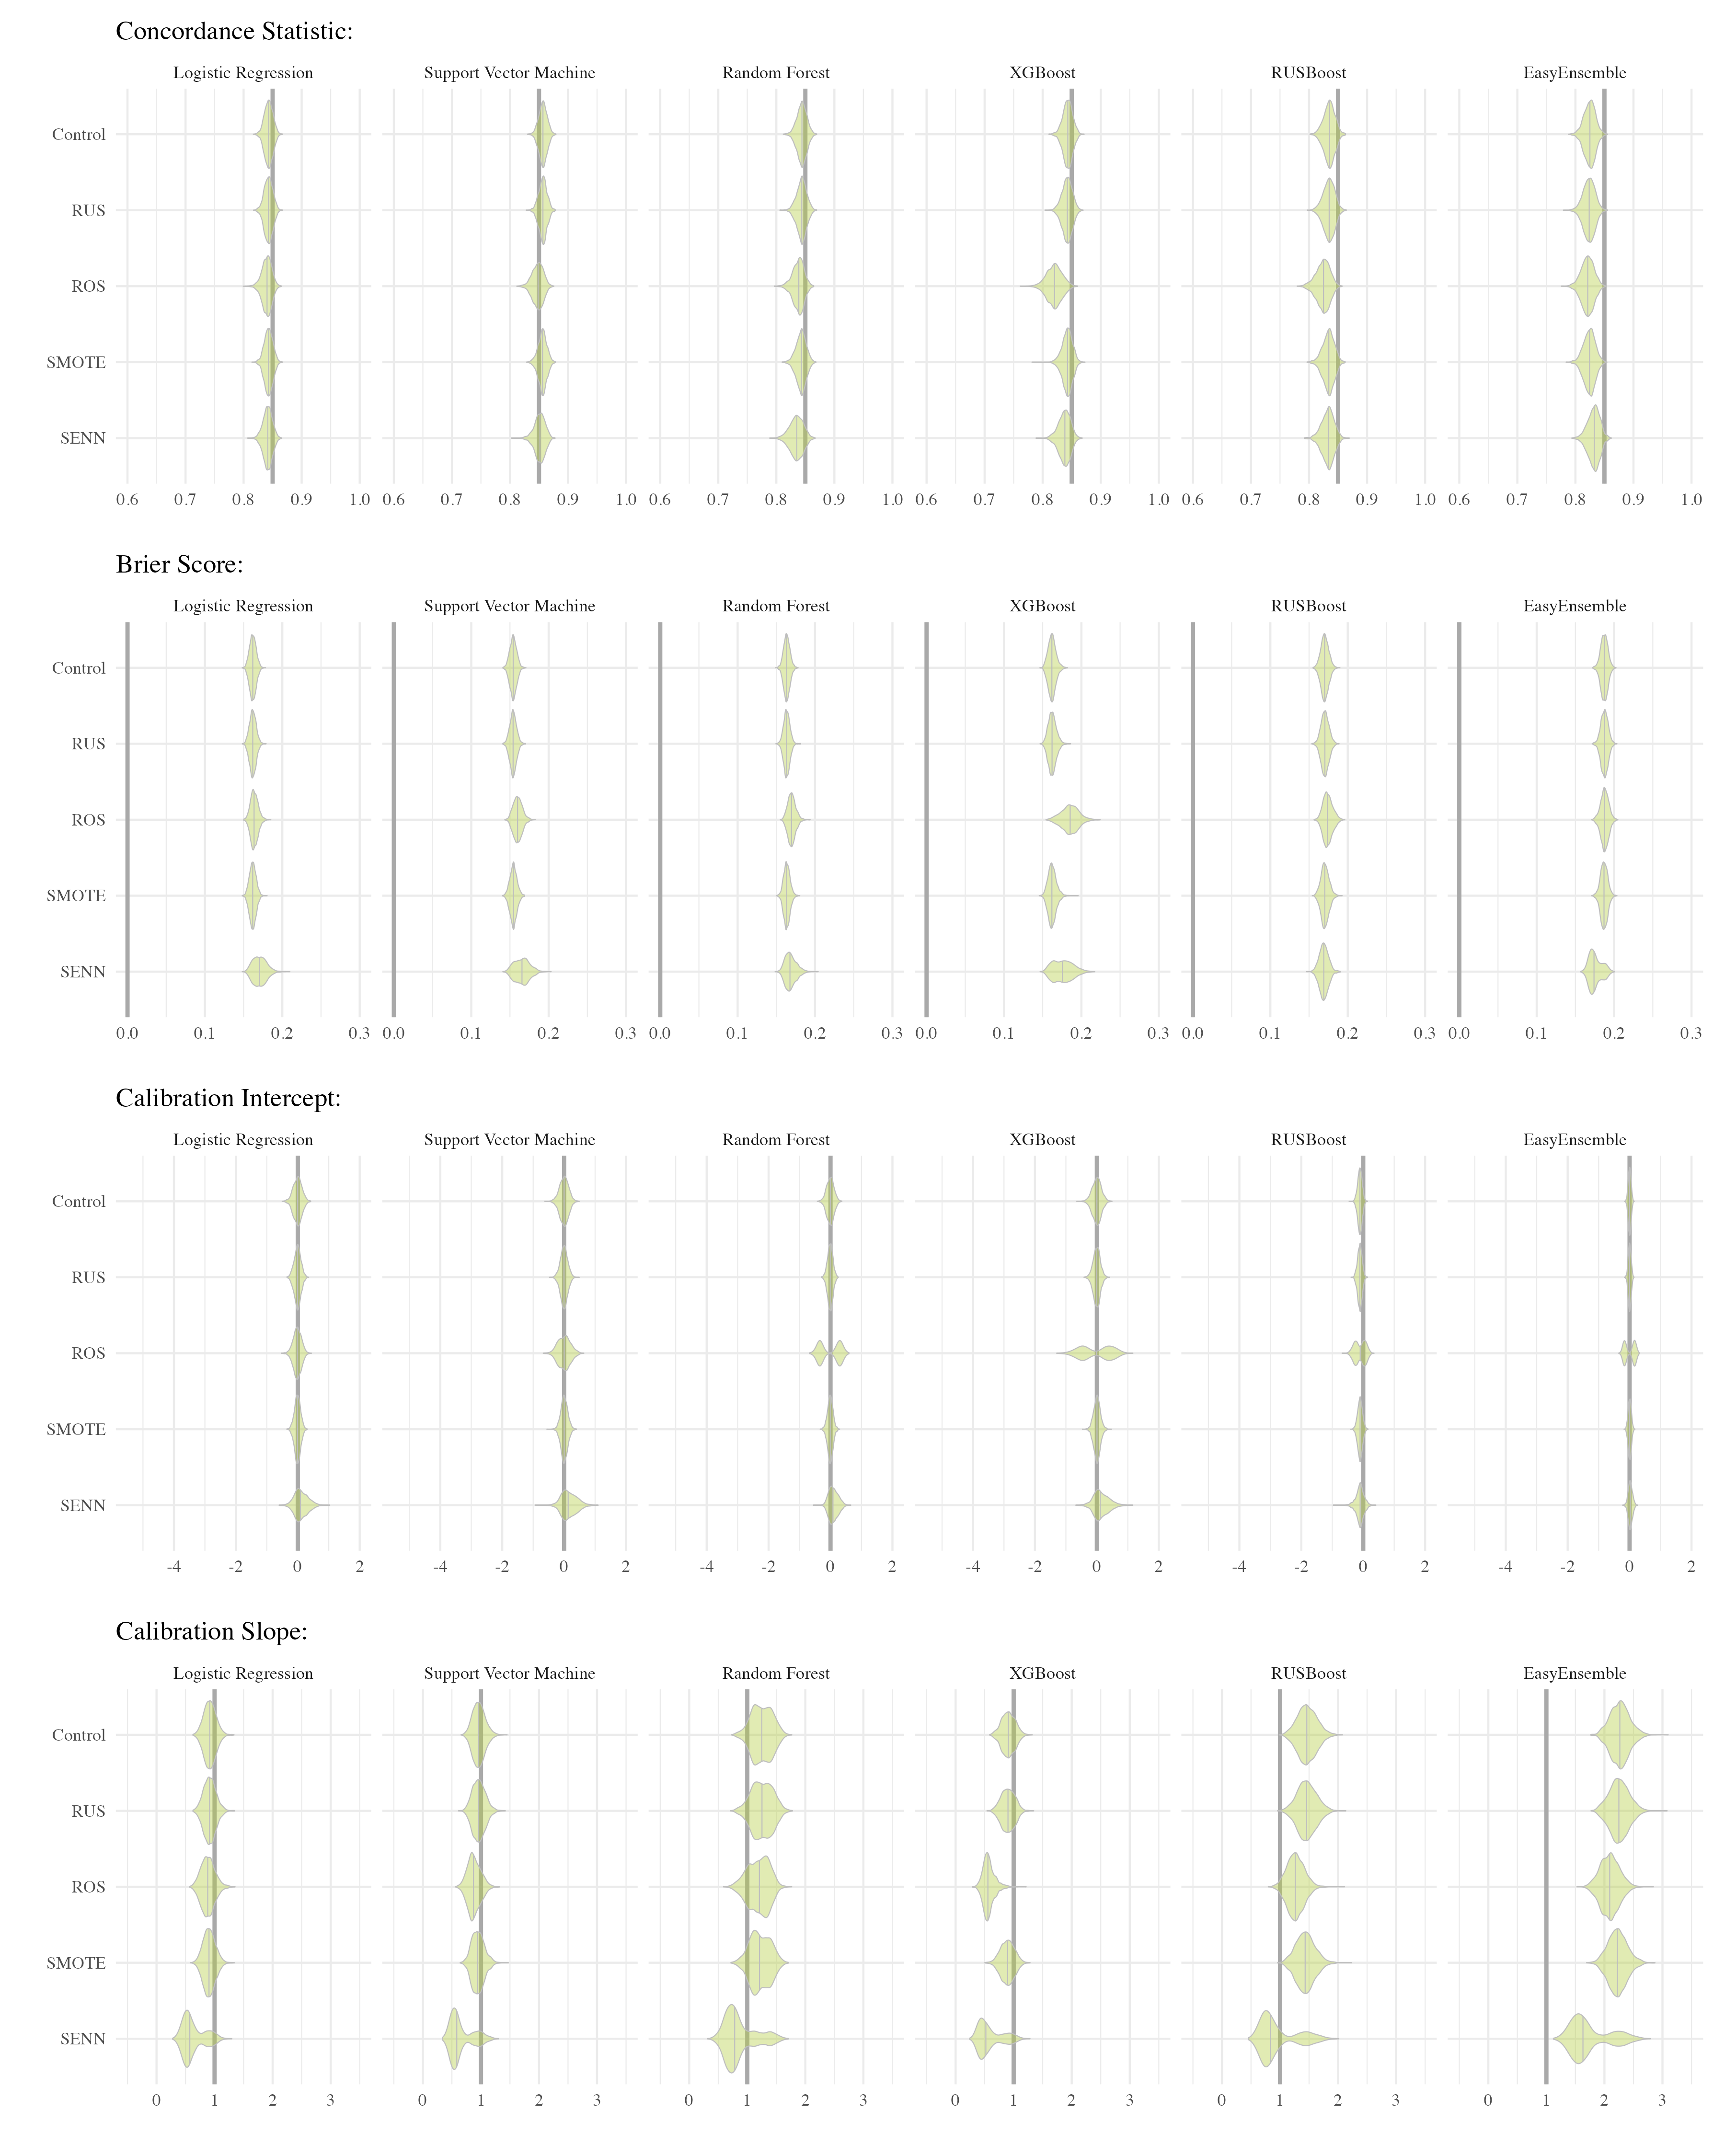
\includegraphics[width=0.7\linewidth]{./figures/performance_metrics_manuscript_sc4} 

}

\caption{Empirical performance metrics for each of 2000 simulation iterations in simulation scenario 4.  This simulation scenario is characterized by 8 predictors, minimum required sample size (N) and class balanced data (event fraction = 0.5). Empirical performance metrics were computed with raw predicted risks; no re-calibration. The target value highlighted for concordance statistic reflects the data-generating concordance statstic, 0.85. Imbalance corrections: RUS (random undersampling), ROS (random oversampling), SMOTE (synthetic majority oversampling), SENN (synthetic majority oversampling with Wilson's Edited Nearest Neighbors). \label{fig:violin_4}}\label{fig:unnamed-chunk-42}
\end{figure}

\begin{figure}

{\centering 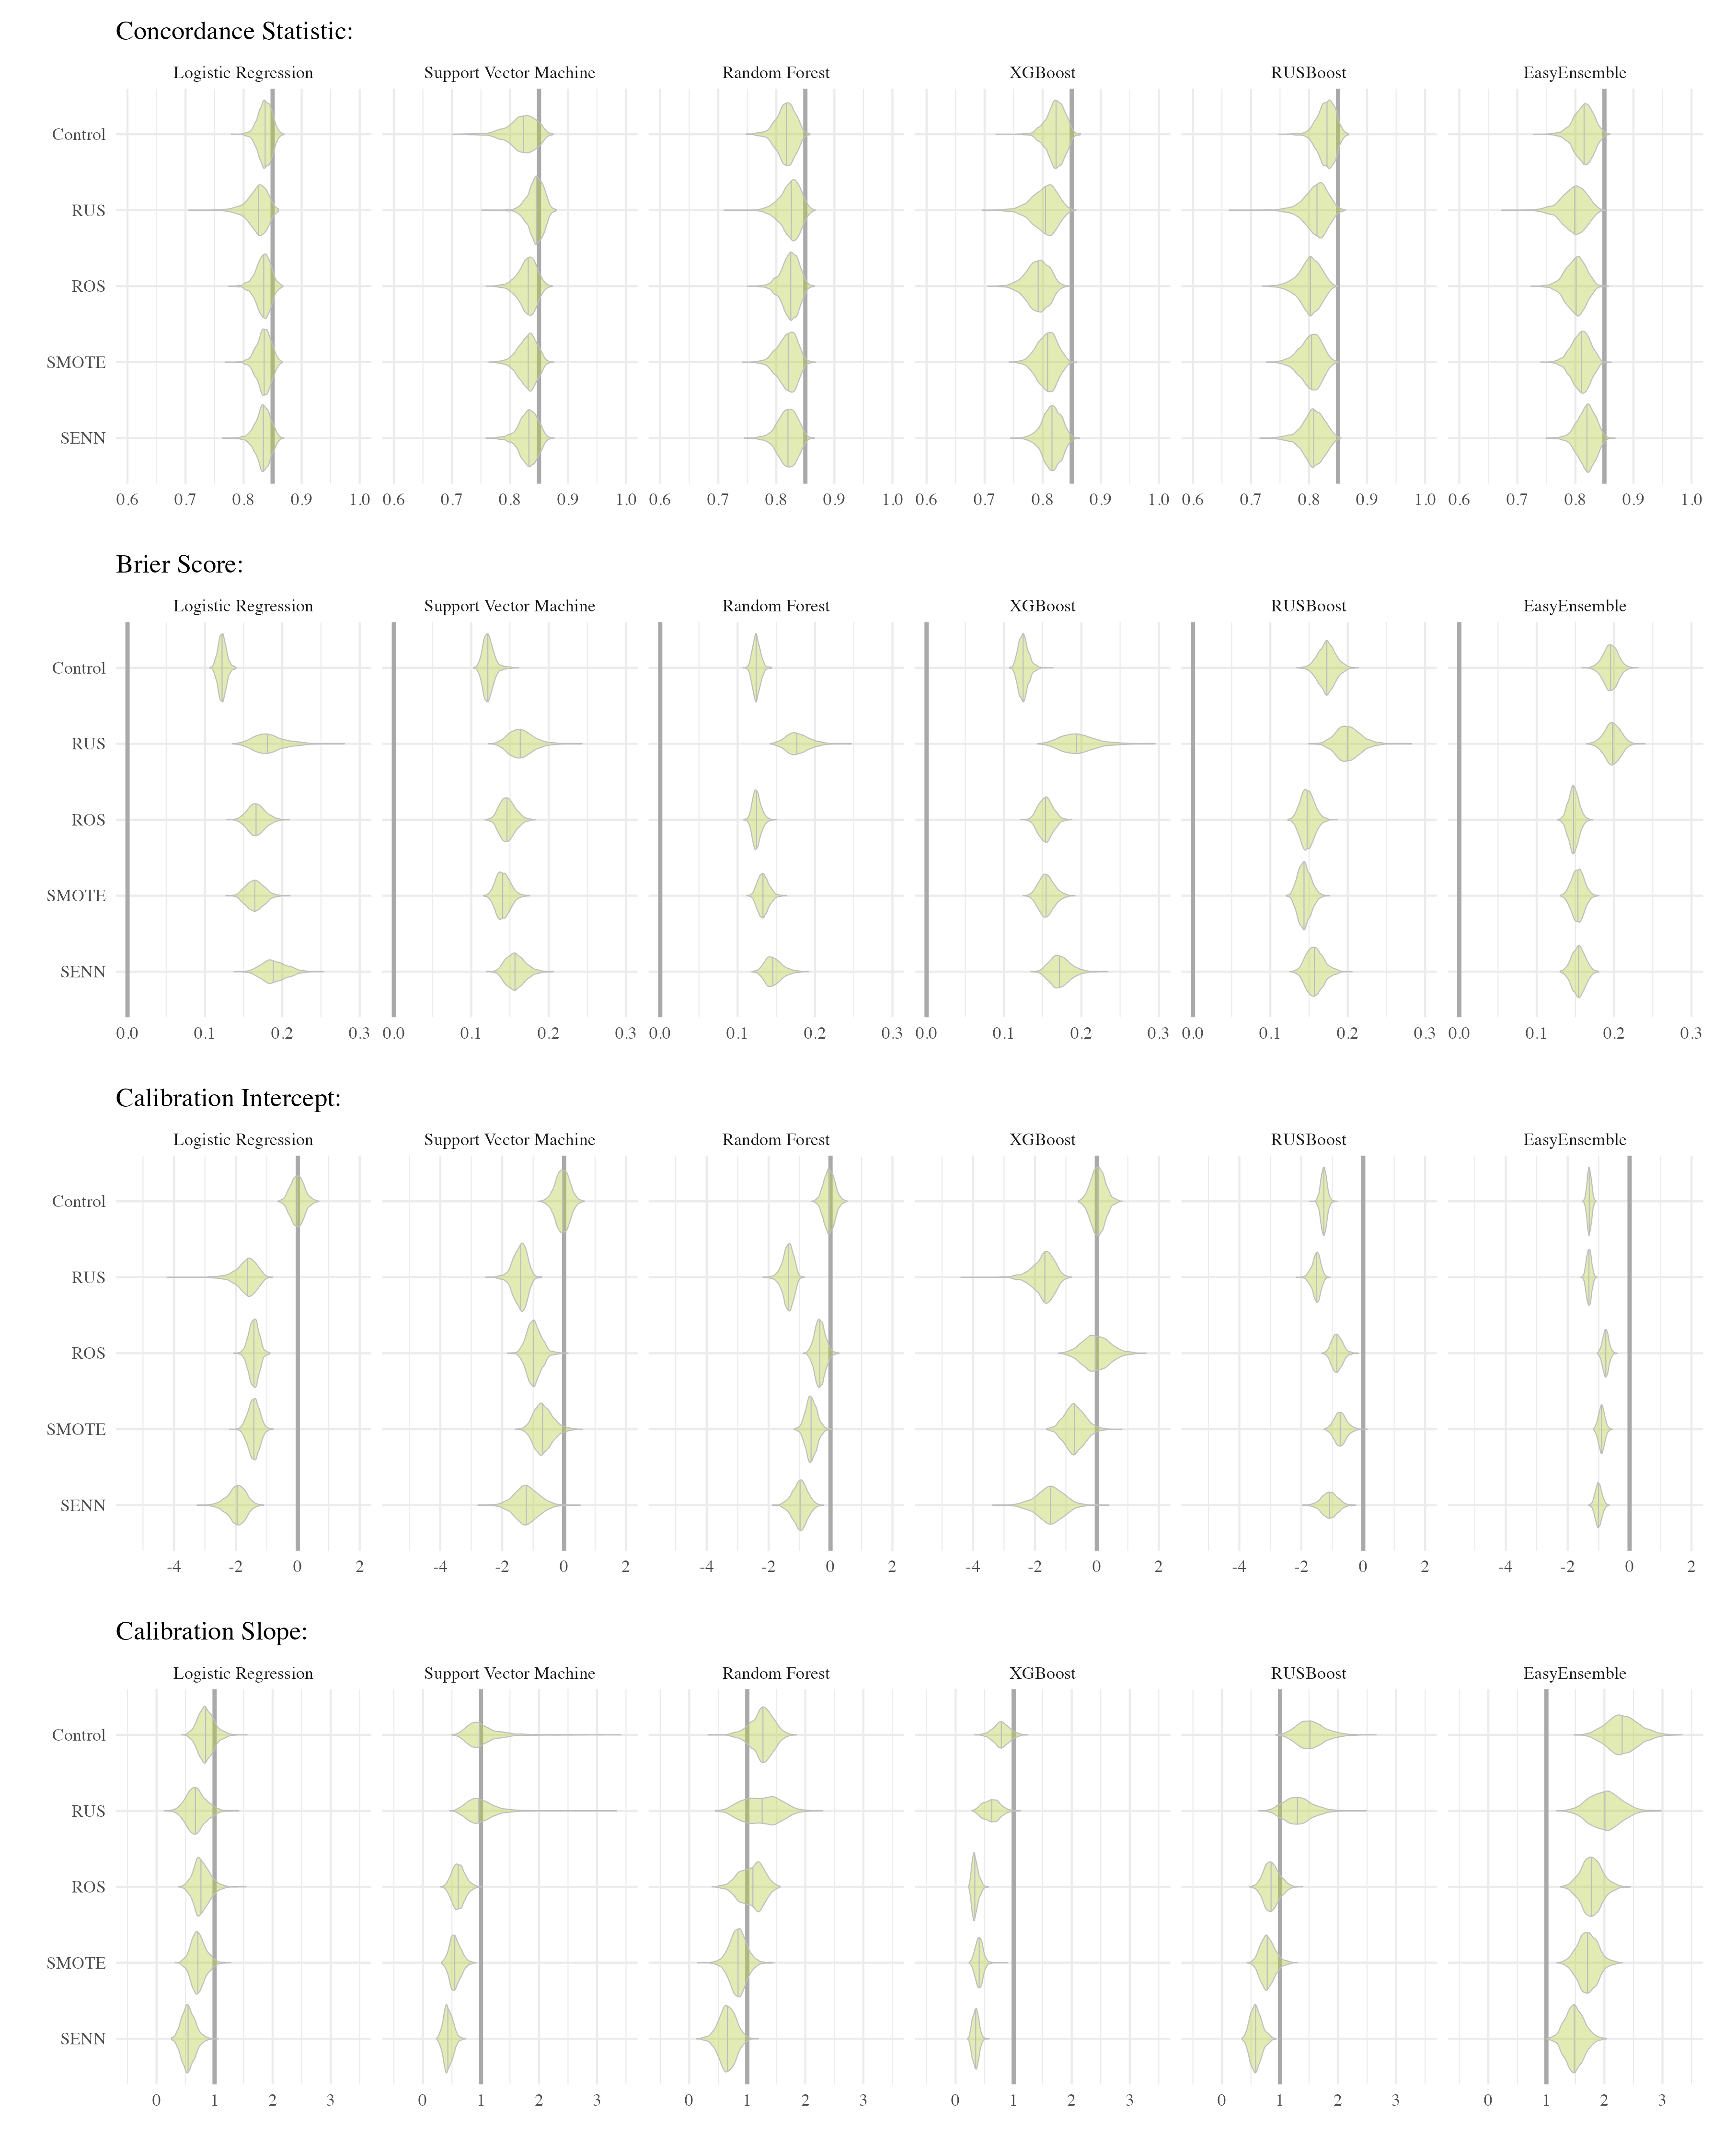
\includegraphics[width=0.7\linewidth]{./figures/performance_metrics_manuscript_sc5} 

}

\caption{Empirical performance metrics for each of 2000 simulation iterations in simulation scenario 5.  This simulation scenario is characterized by 8 predictors, minimum required sample size (N) and moderately imbalanced data (event fraction = 0.2). Empirical performance metrics were computed with raw predicted risks; no re-calibration. The target value highlighted for concordance statistic reflects the data-generating concordance statstic, 0.85. Imbalance corrections: RUS (random undersampling), ROS (random oversampling), SMOTE (synthetic majority oversampling), SENN (synthetic majority oversampling with Wilson's Edited Nearest Neighbors).\label{fig:violin_5}}\label{fig:unnamed-chunk-43}
\end{figure}

\begin{figure}

{\centering 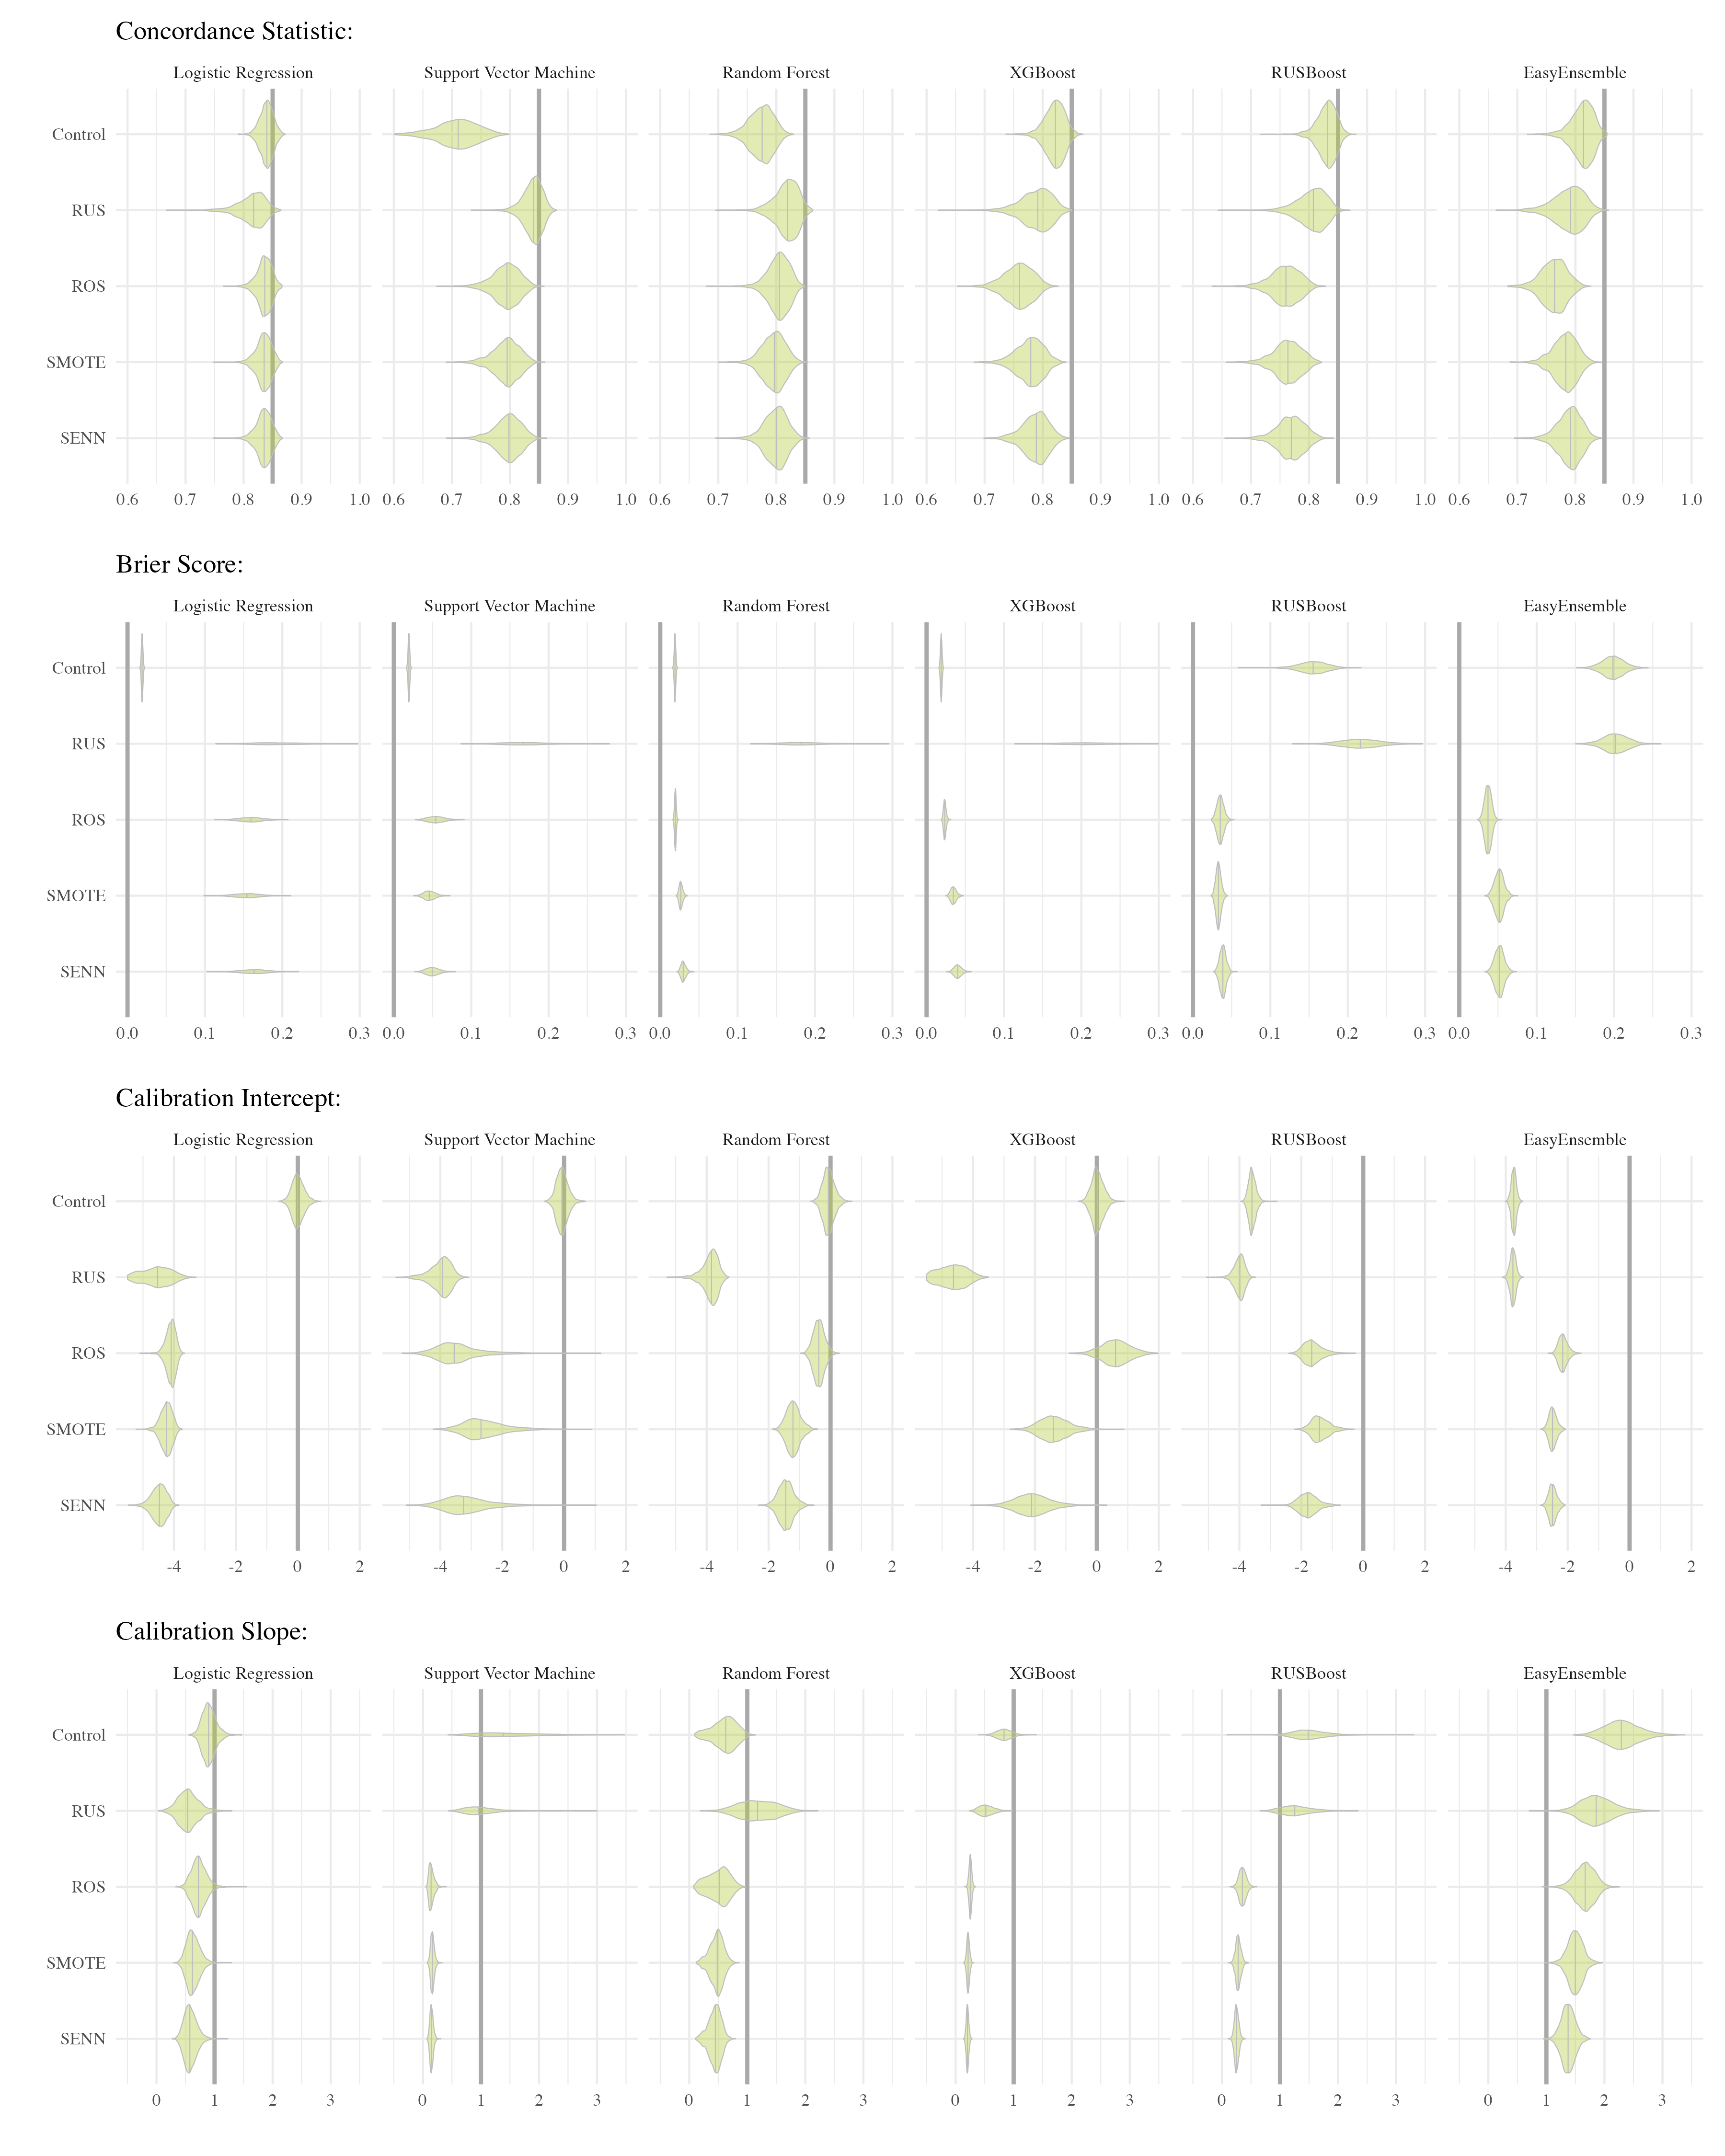
\includegraphics[width=0.7\linewidth]{./figures/performance_metrics_manuscript_sc6} 

}

\caption{Empirical performance metrics for each of 2000 simulation iterations in simulation scenario 6.  This simulation scenario is characterized by 8 predictors, minimum required sample size (N) and strongly imbalanced data (event fraction = 0.02). Empirical performance metrics were computed with raw predicted risks; no re-calibration. The target value highlighted for concordance statistic reflects the data-generating concordance statstic, 0.85. Imbalance corrections: RUS (random undersampling), ROS (random oversampling), SMOTE (synthetic majority oversampling), SENN (synthetic majority oversampling with Wilson's Edited Nearest Neighbors).\label{fig:violin_6}}\label{fig:unnamed-chunk-44}
\end{figure}

\begin{figure}

{\centering 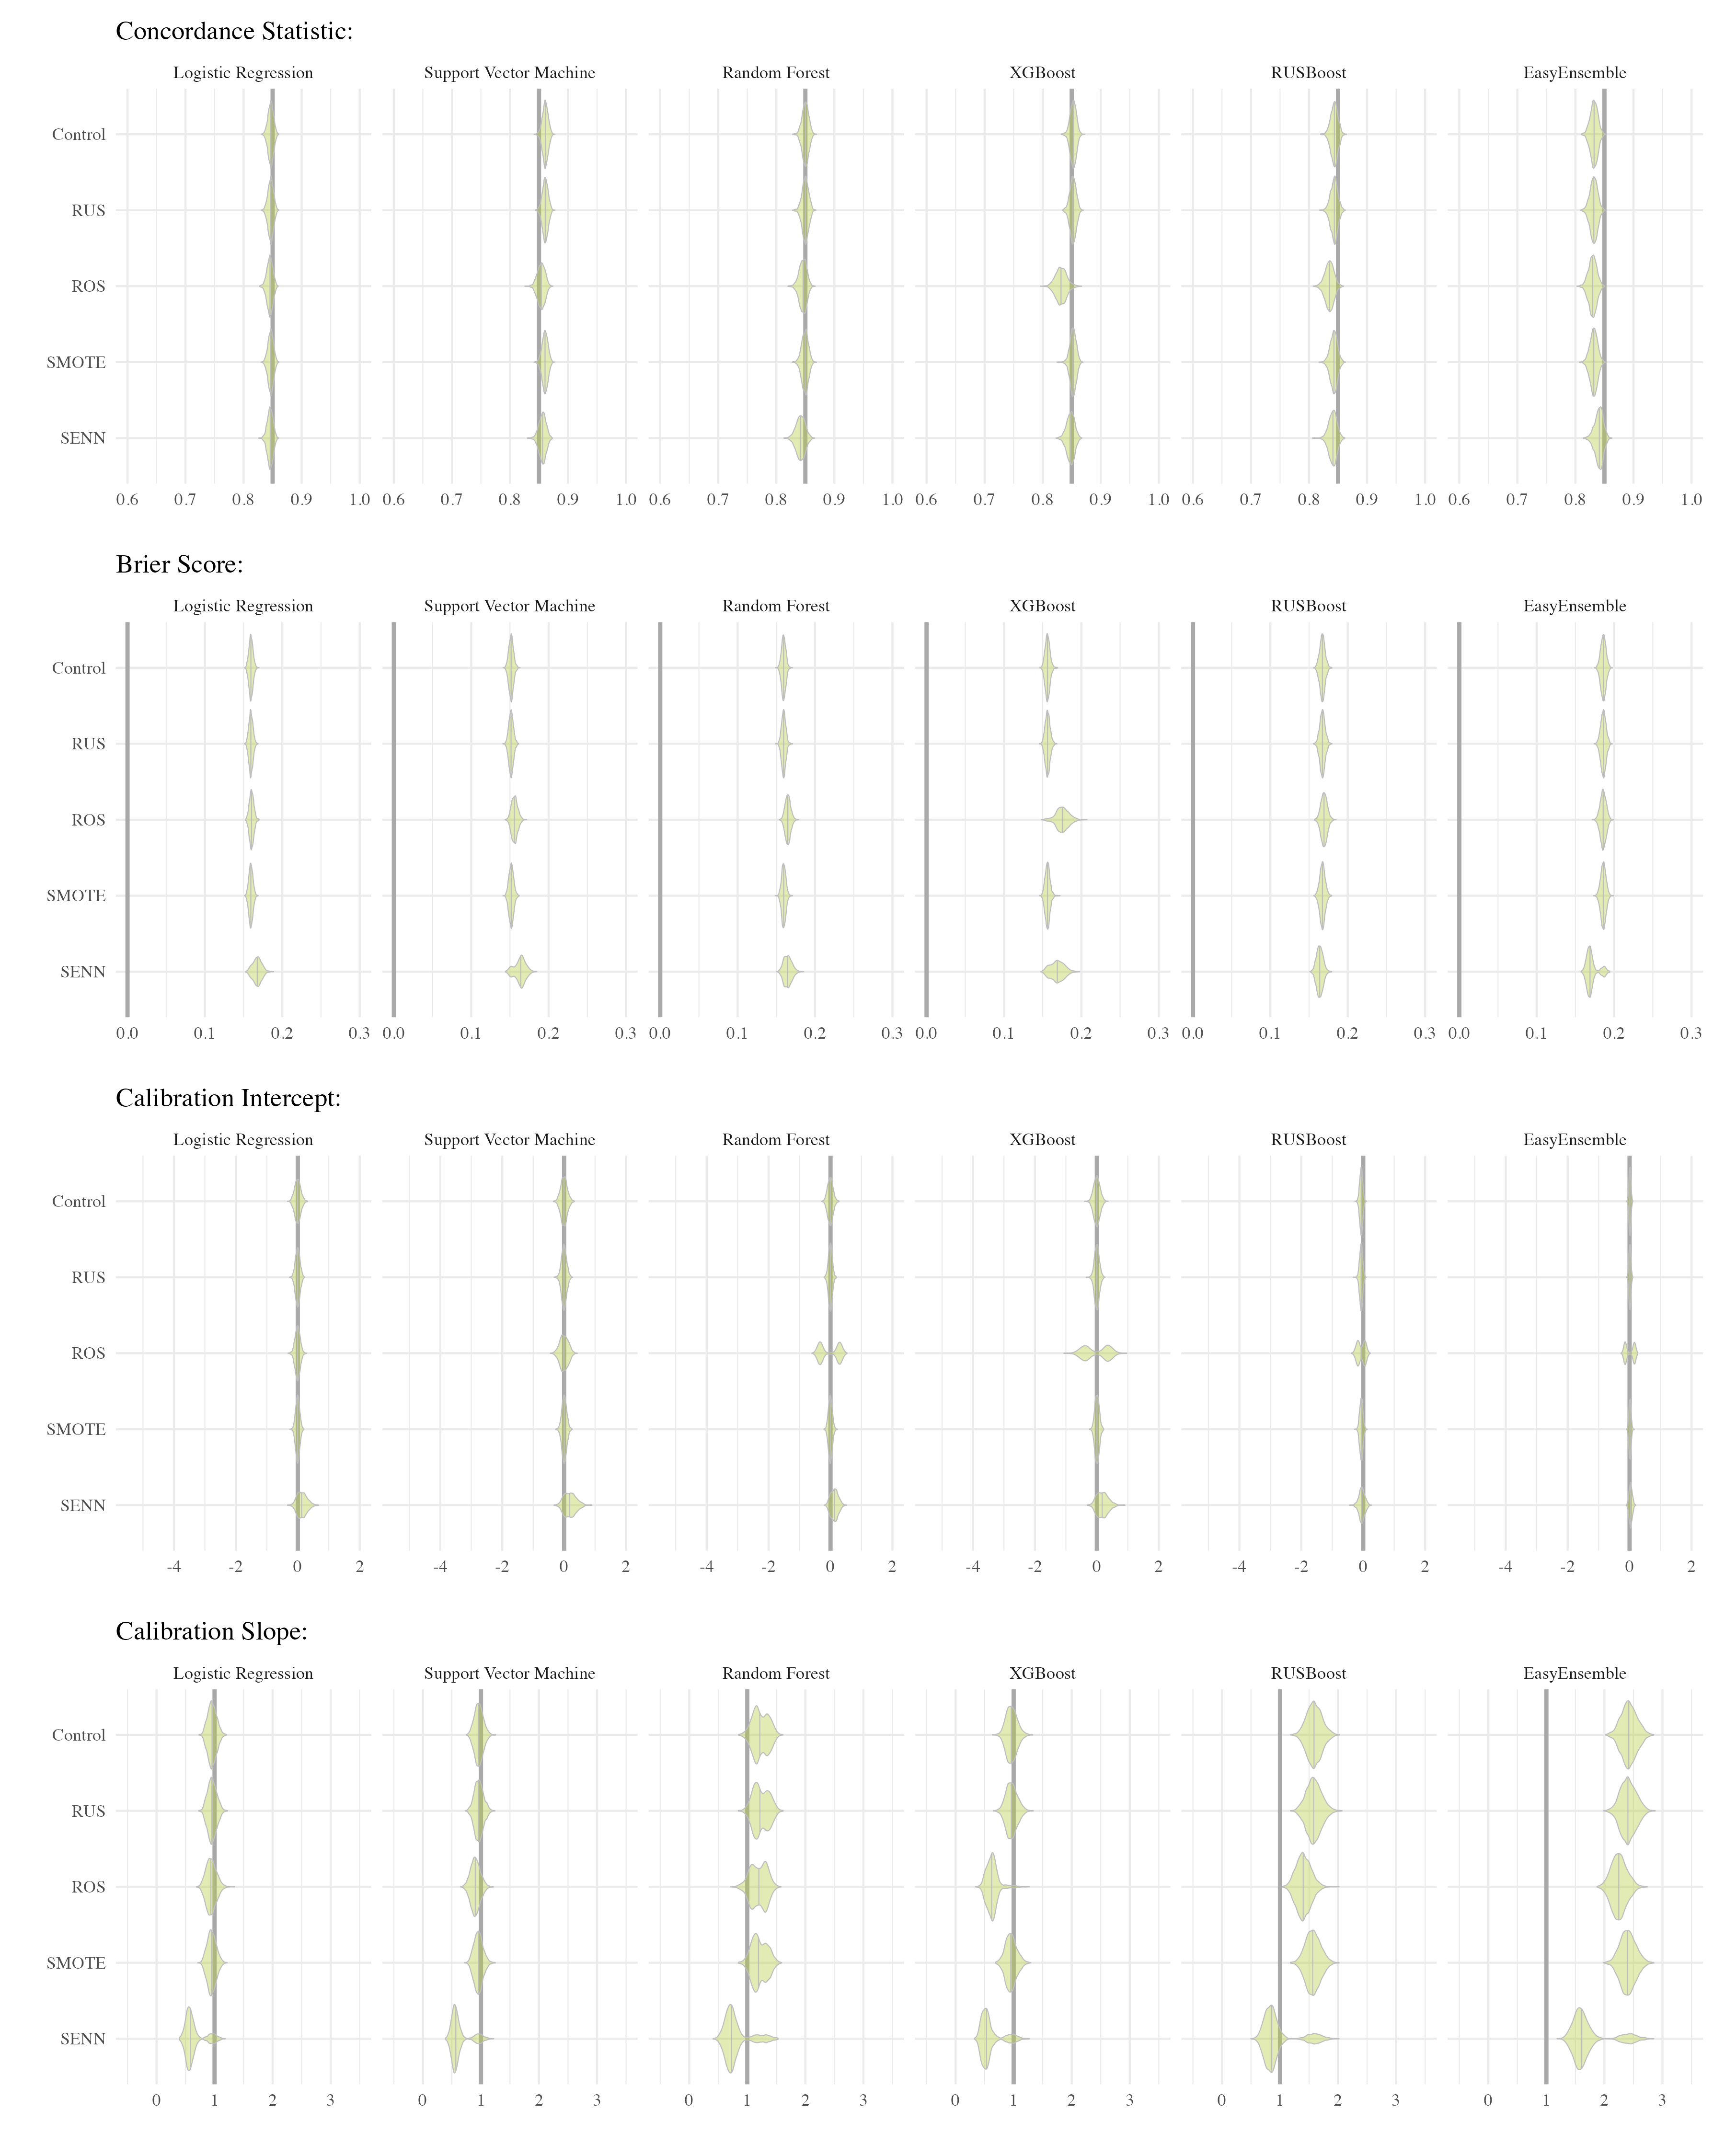
\includegraphics[width=0.7\linewidth]{./figures/performance_metrics_manuscript_sc7} 

}

\caption{Empirical performance metrics for each of 2000 simulation iterations in simulation scenario 7.  This simulation scenario is characterized by 8 predictors, double the required sample size (2N) and class balanced data (event fraction = 0.5). Empirical performance metrics were computed with raw predicted risks; no re-calibration. The target value highlighted for concordance statistic reflects the data-generating concordance statstic, 0.85. Imbalance corrections: RUS (random undersampling), ROS (random oversampling), SMOTE (synthetic majority oversampling), SENN (synthetic majority oversampling with Wilson's Edited Nearest Neighbors). \label{fig:violin_7}}\label{fig:unnamed-chunk-45}
\end{figure}

\begin{figure}

{\centering 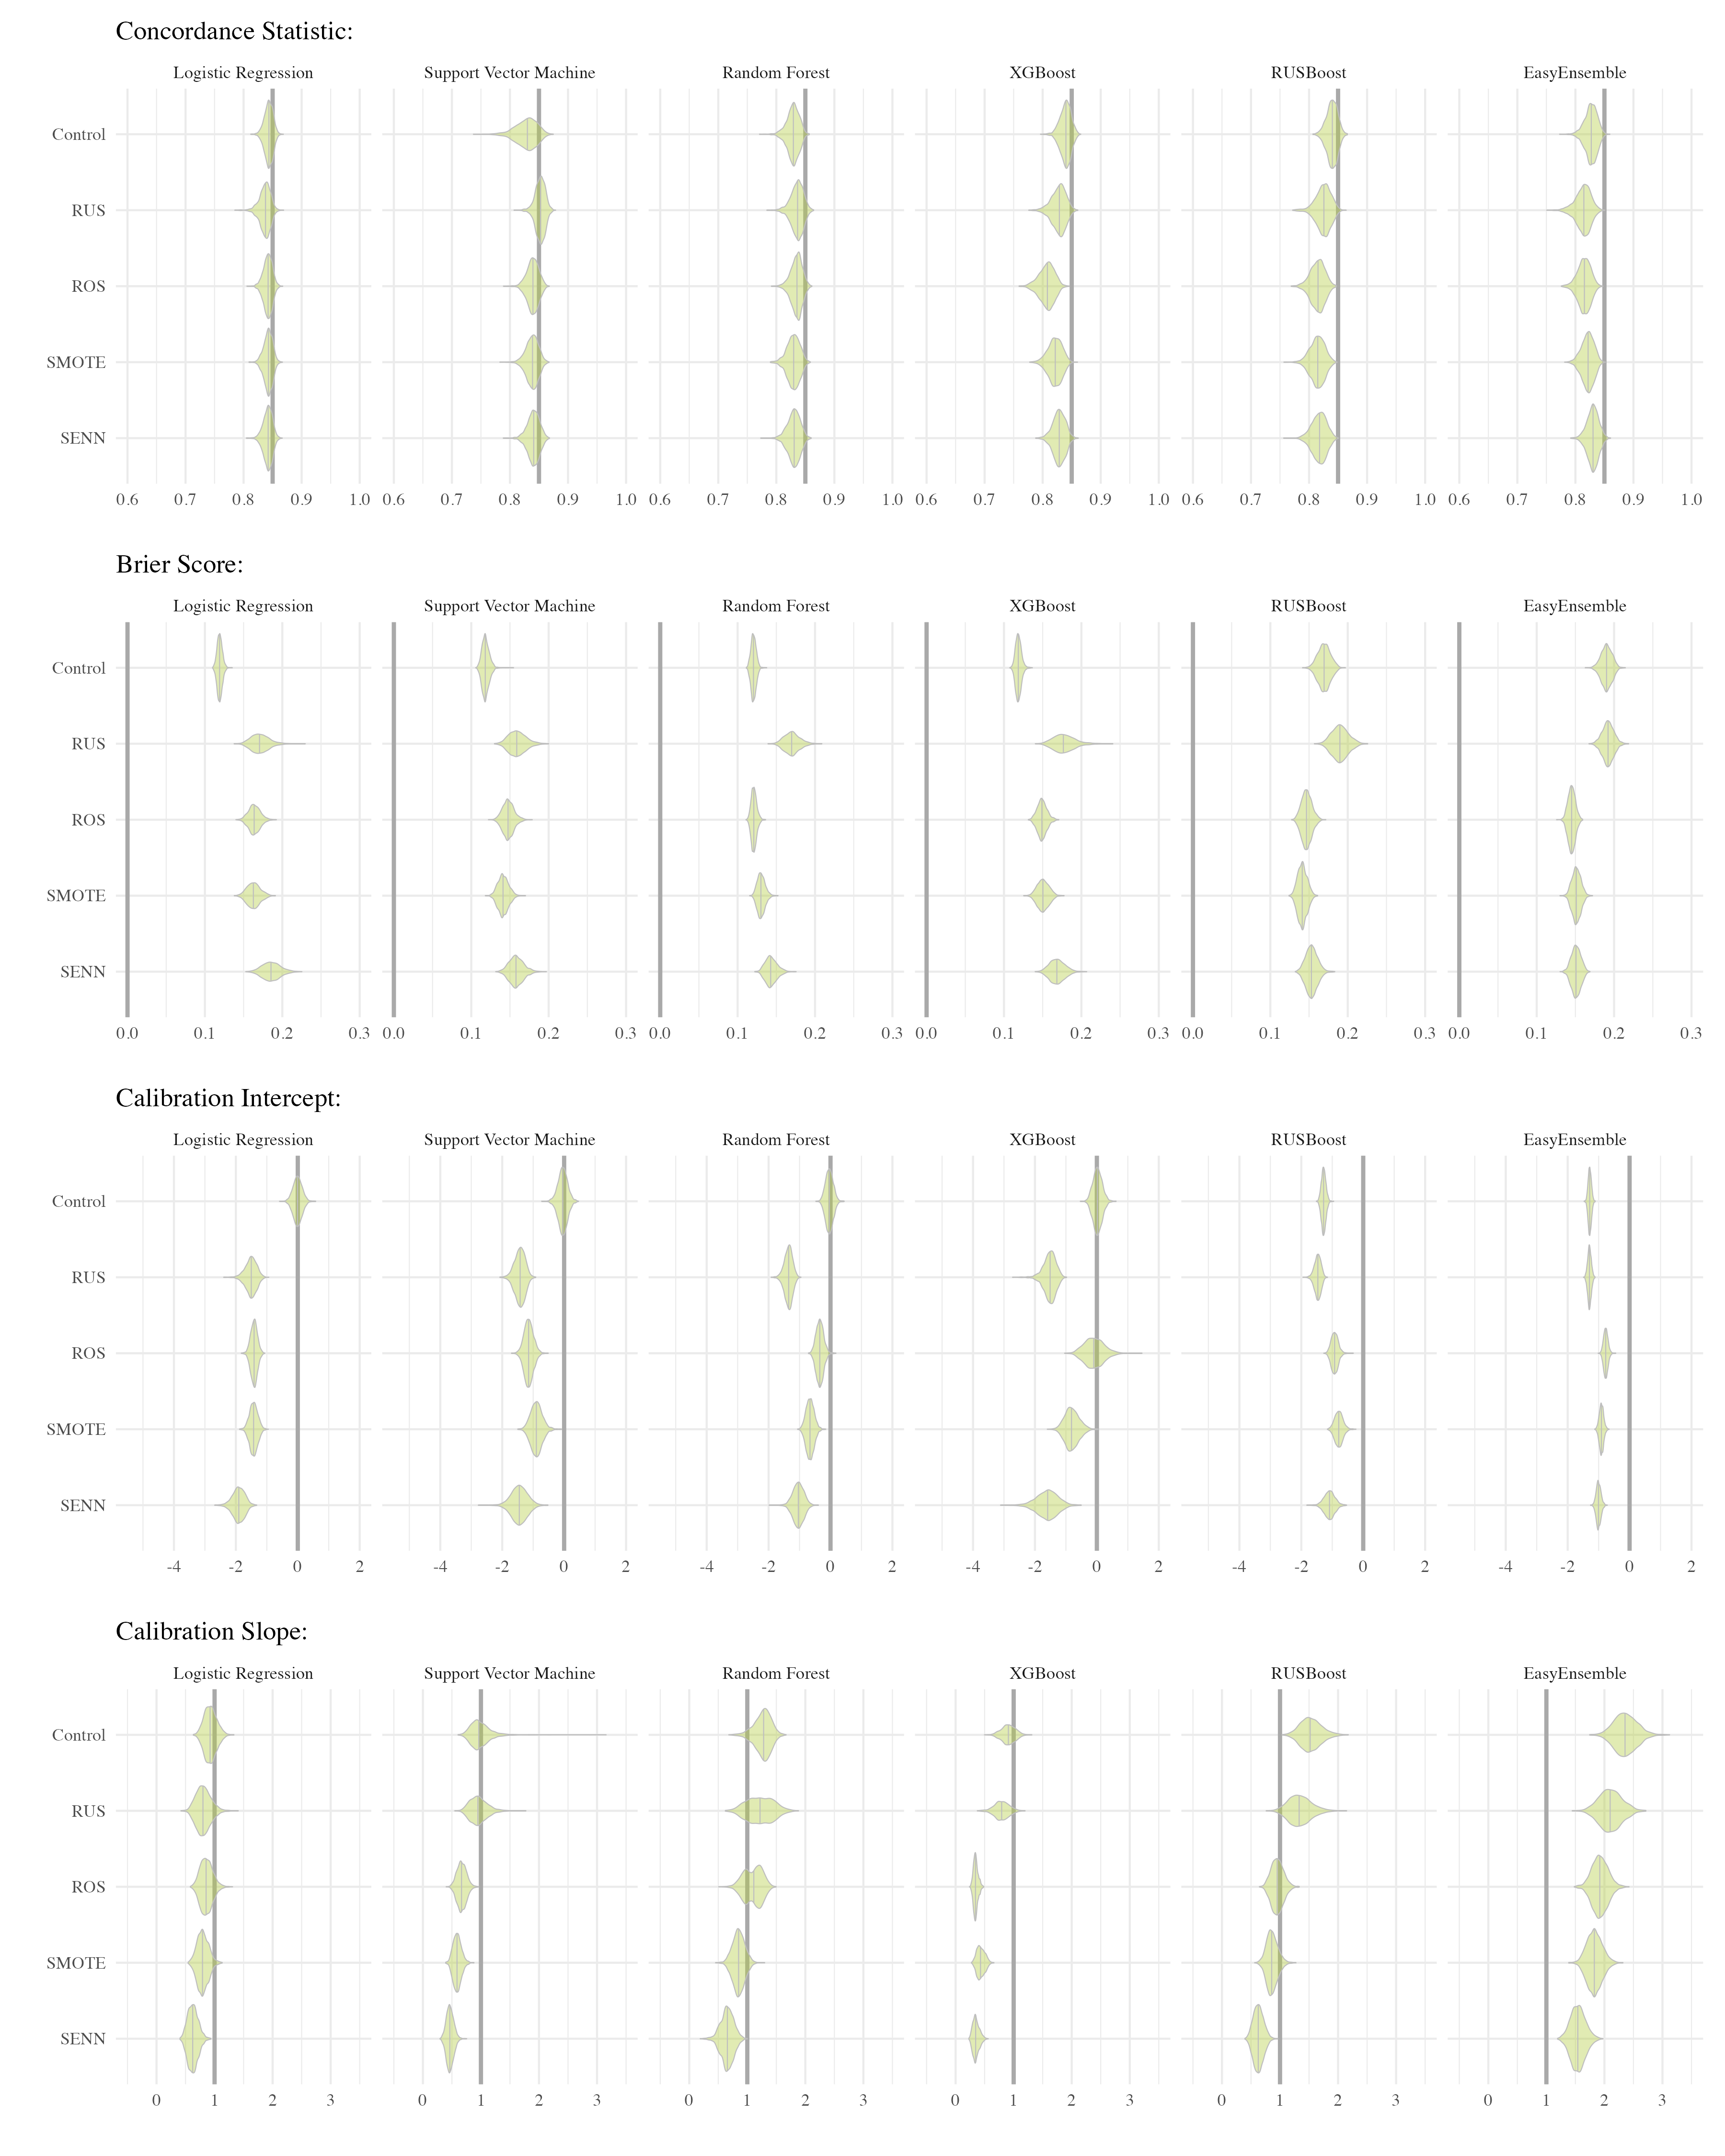
\includegraphics[width=0.7\linewidth]{./figures/performance_metrics_manuscript_sc8} 

}

\caption{Empirical performance metrics for each of 2000 simulation iterations in simulation scenario 8.  This simulation scenario is characterized by 8 predictors, double the required sample size (2N) and moderately imbalanced data (event fraction = 0.2).  Empirical performance metrics were computed with raw predicted risks; no re-calibration. The target value highlighted for concordance statistic reflects the data-generating concordance statstic, 0.85. Imbalance corrections: RUS (random undersampling), ROS (random oversampling), SMOTE (synthetic majority oversampling), SENN (synthetic majority oversampling with Wilson's Edited Nearest Neighbors). \label{fig:violin_8}}\label{fig:unnamed-chunk-46}
\end{figure}

\begin{figure}

{\centering 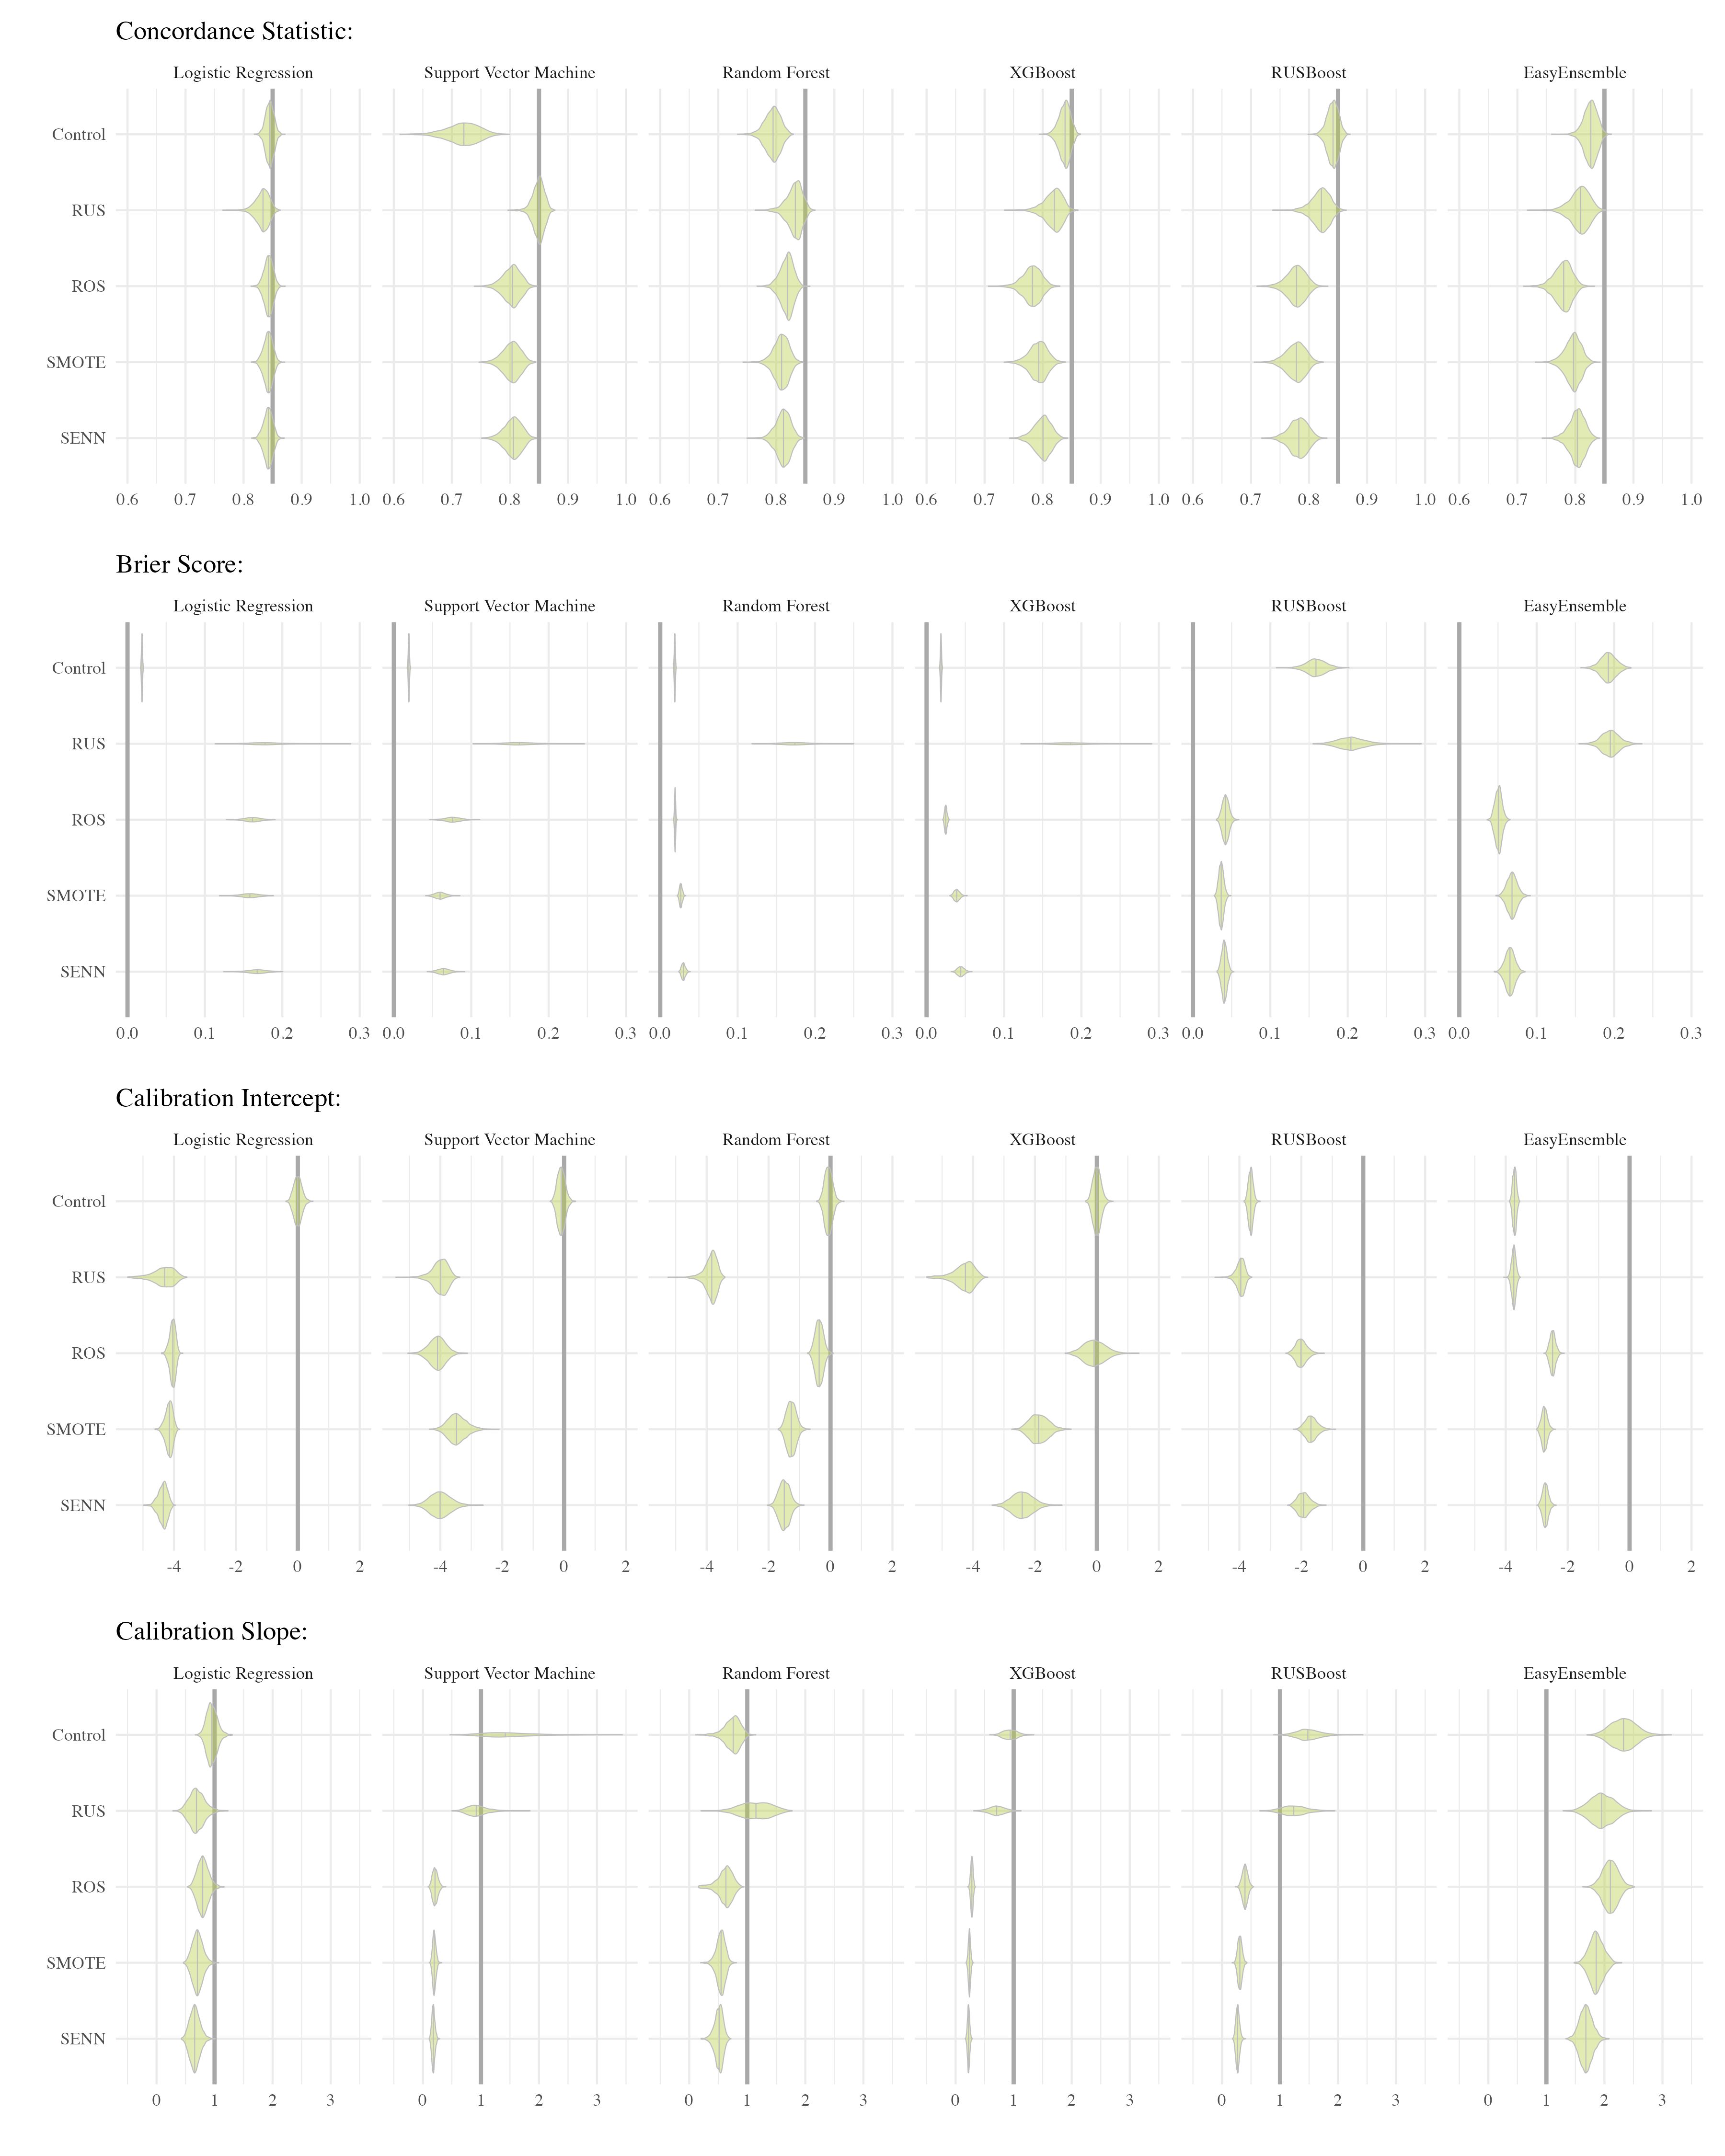
\includegraphics[width=0.7\linewidth]{./figures/performance_metrics_manuscript_sc9} 

}

\caption{Empirical performance metrics for each of 2000 simulation iterations in simulation scenario 9.  This simulation scenario is characterized by 8 predictors, double the required sample size (2N) and strongly imbalanced data (event fraction = 0.02). Empirical performance metrics were computed with raw predicted risks; no re-calibration. The target value highlighted for concordance statistic reflects the data-generating concordance statstic, 0.85. Imbalance corrections: RUS (random undersampling), ROS (random oversampling), SMOTE (synthetic majority oversampling), SENN (synthetic majority oversampling with Wilson's Edited Nearest Neighbors). \label{fig:violin_9}}\label{fig:unnamed-chunk-47}
\end{figure}

\begin{figure}

{\centering 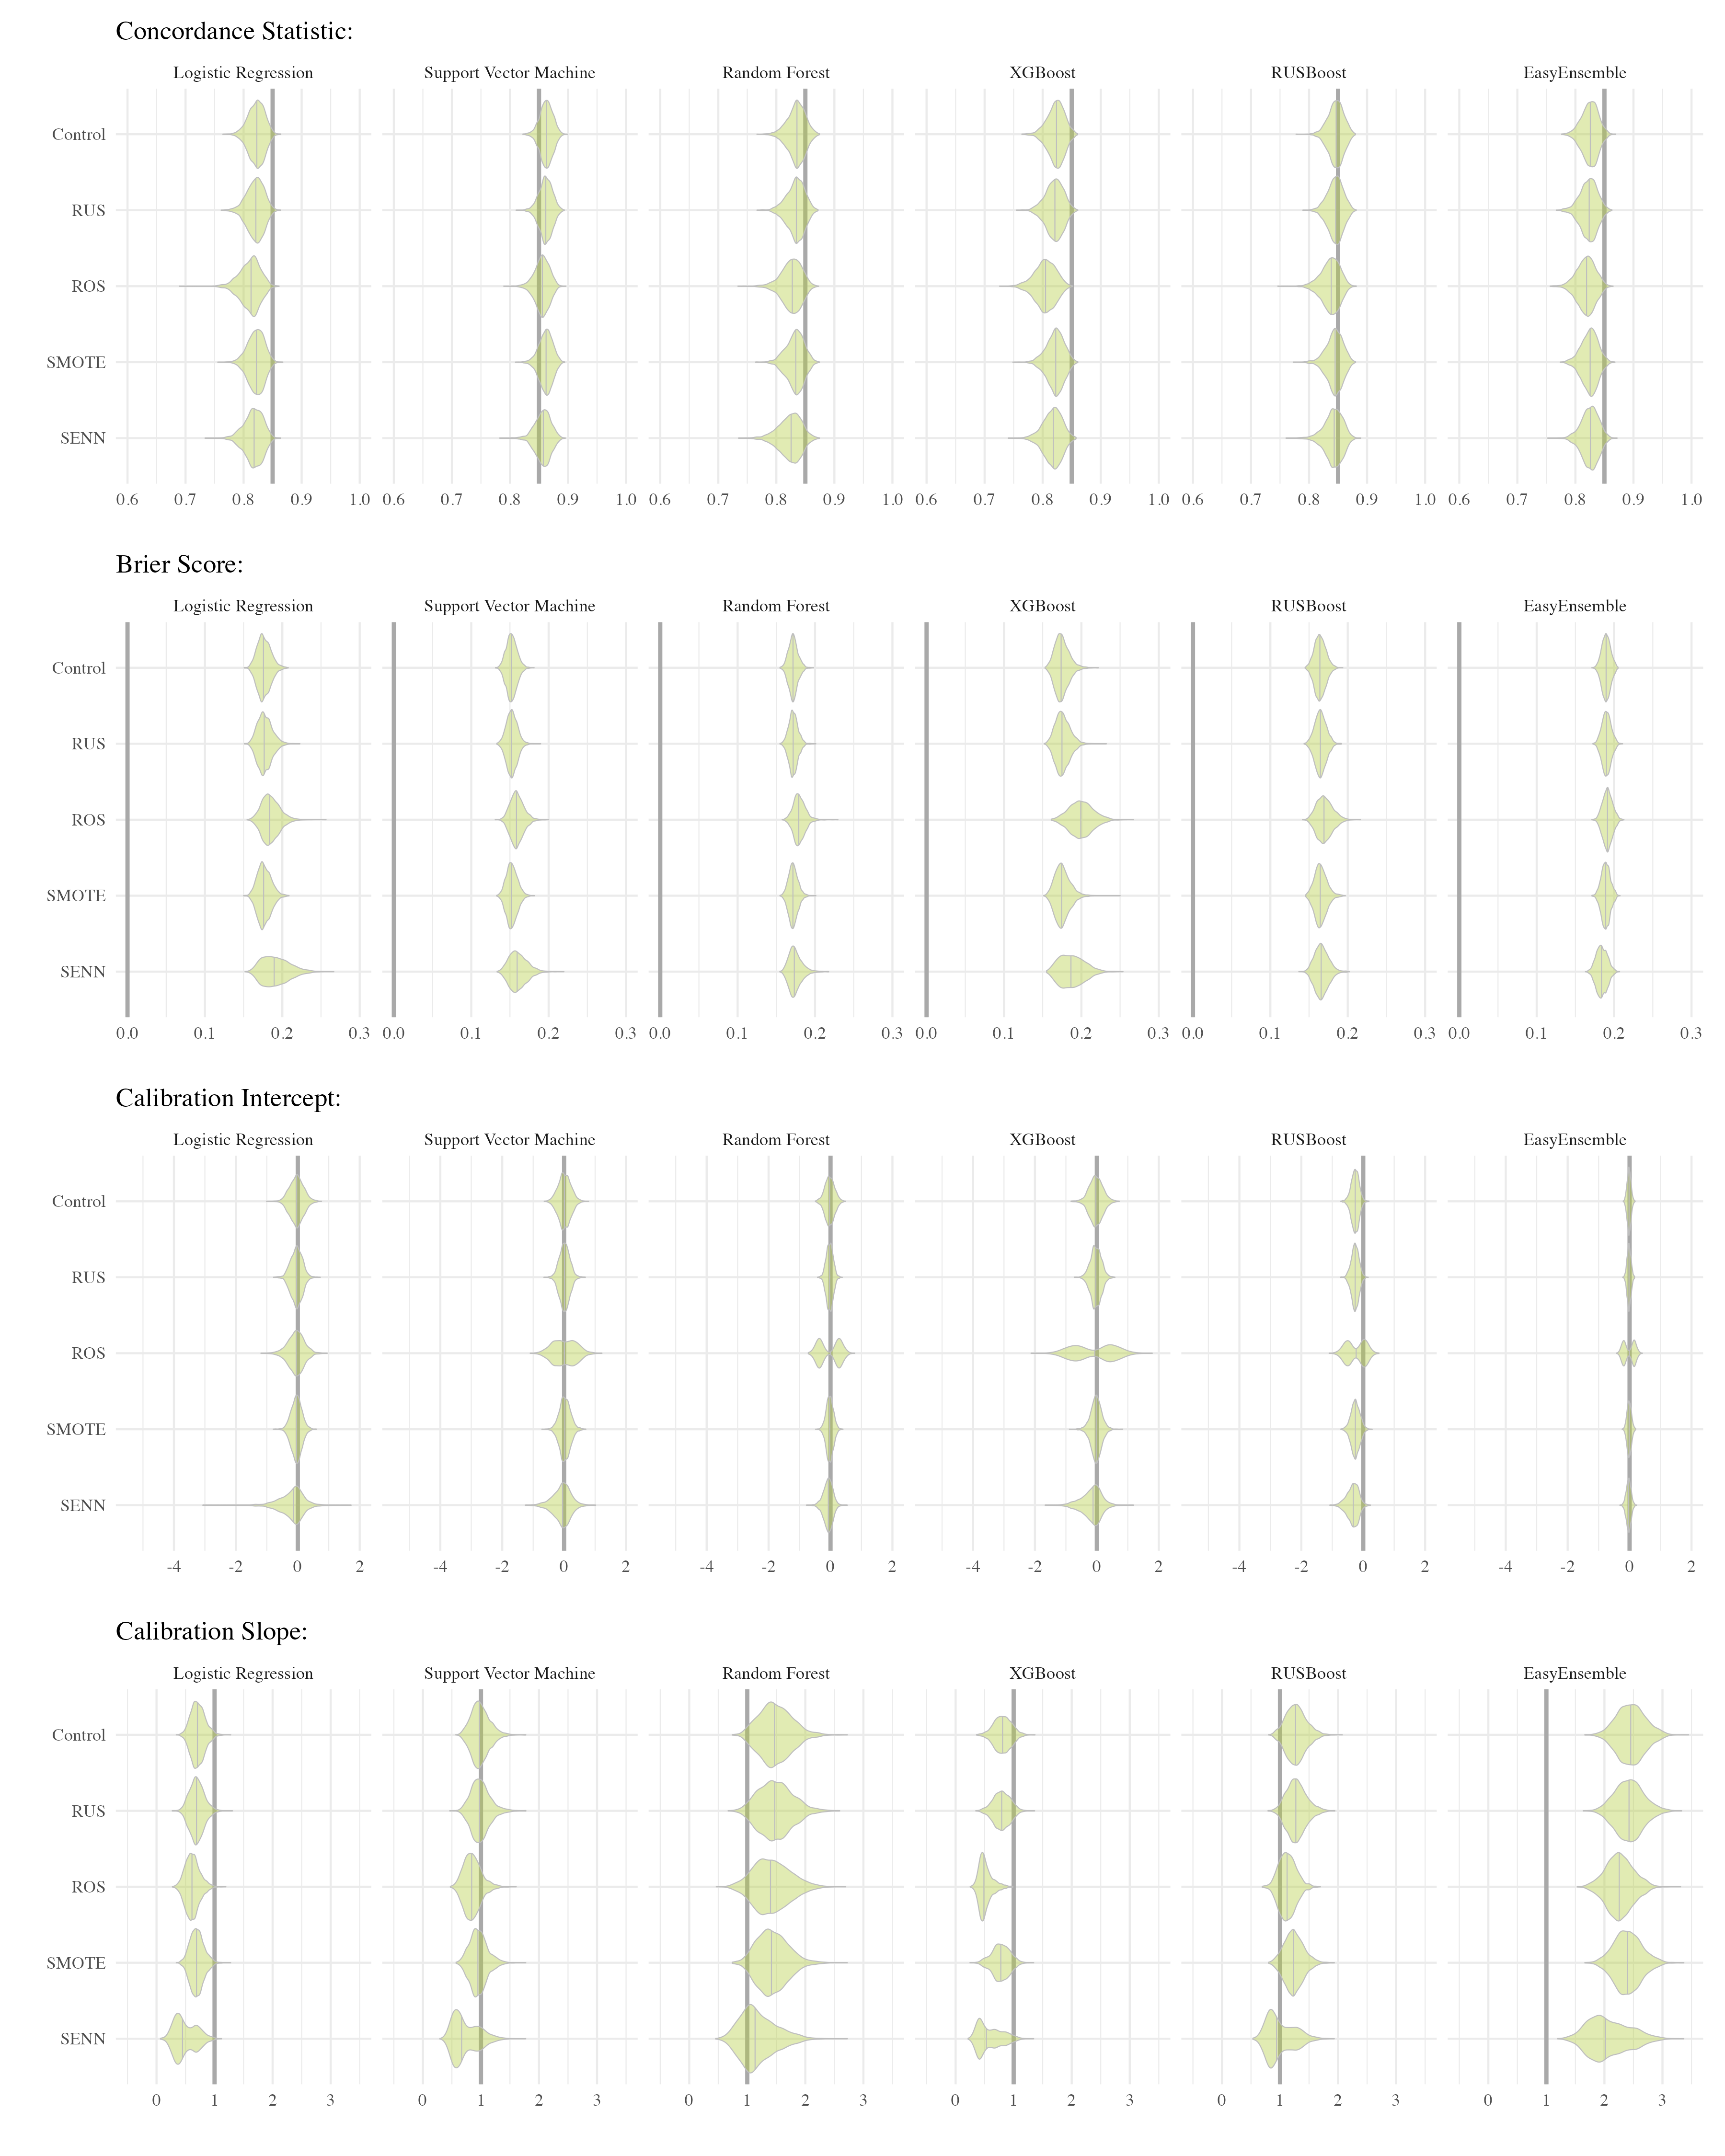
\includegraphics[width=0.7\linewidth]{./figures/performance_metrics_manuscript_sc10} 

}

\caption{Empirical performance metrics for each of 2000 simulation iterations in simulation scenario 10.  This simulation scenario is characterized by 16 predictors, half the required sample size (0.5N) and class balanced data (event fraction = 0.5). Empirical performance metrics were computed with raw predicted risks; no re-calibration. The target value highlighted for concordance statistic reflects the data-generating concordance statstic, 0.85. Imbalance corrections: RUS (random undersampling), ROS (random oversampling), SMOTE (synthetic majority oversampling), SENN (synthetic majority oversampling with Wilson's Edited Nearest Neighbors).  \label{fig:violin_10}}\label{fig:unnamed-chunk-48}
\end{figure}

\begin{figure}

{\centering 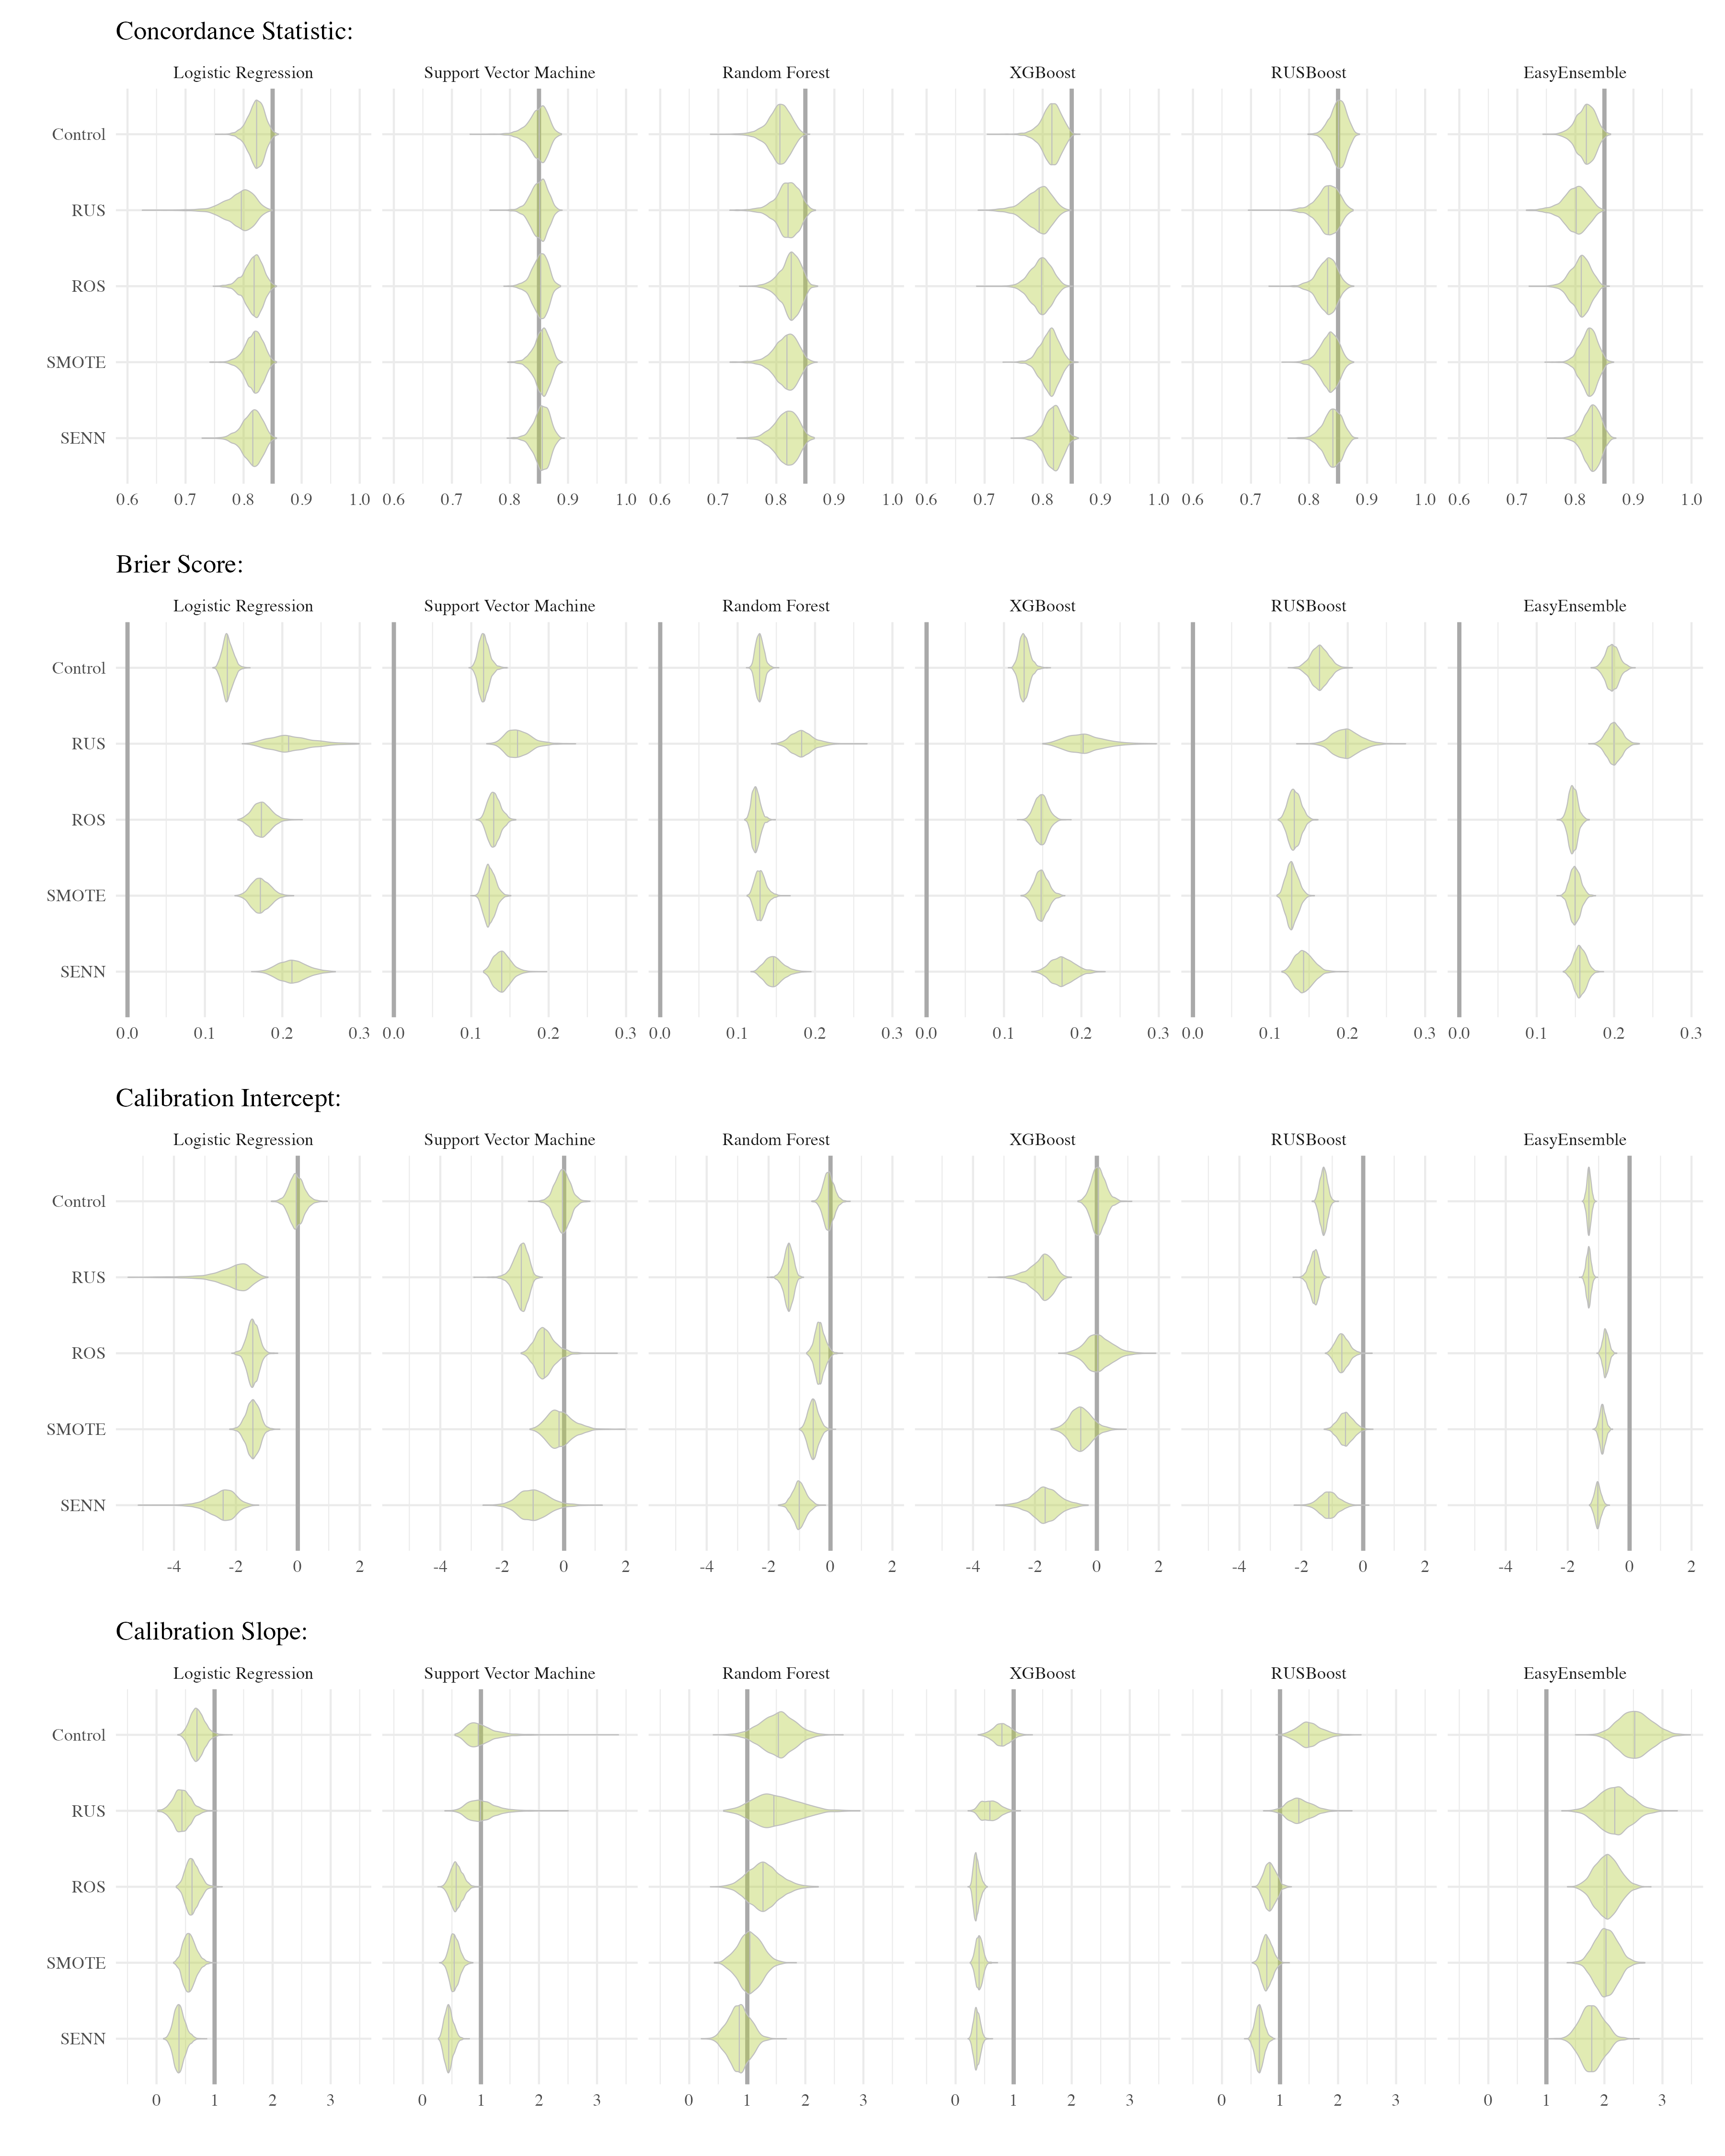
\includegraphics[width=0.7\linewidth]{./figures/performance_metrics_manuscript_sc11} 

}

\caption{Empirical performance metrics for each of 2000 simulation iterations in simulation scenario 11.  This simulation scenario is characterized by 16 predictors, half the required sample size (0.5N) and moderately imbalanced data (event fraction = 0.2). Empirical performance metrics were computed with raw predicted risks; no re-calibration. The target value highlighted for concordance statistic reflects the data-generating concordance statstic, 0.85. Imbalance corrections: RUS (random undersampling), ROS (random oversampling), SMOTE (synthetic majority oversampling), SENN (synthetic majority oversampling with Wilson's Edited Nearest Neighbors). \label{fig:violin_11}}\label{fig:unnamed-chunk-49}
\end{figure}

\begin{figure}

{\centering 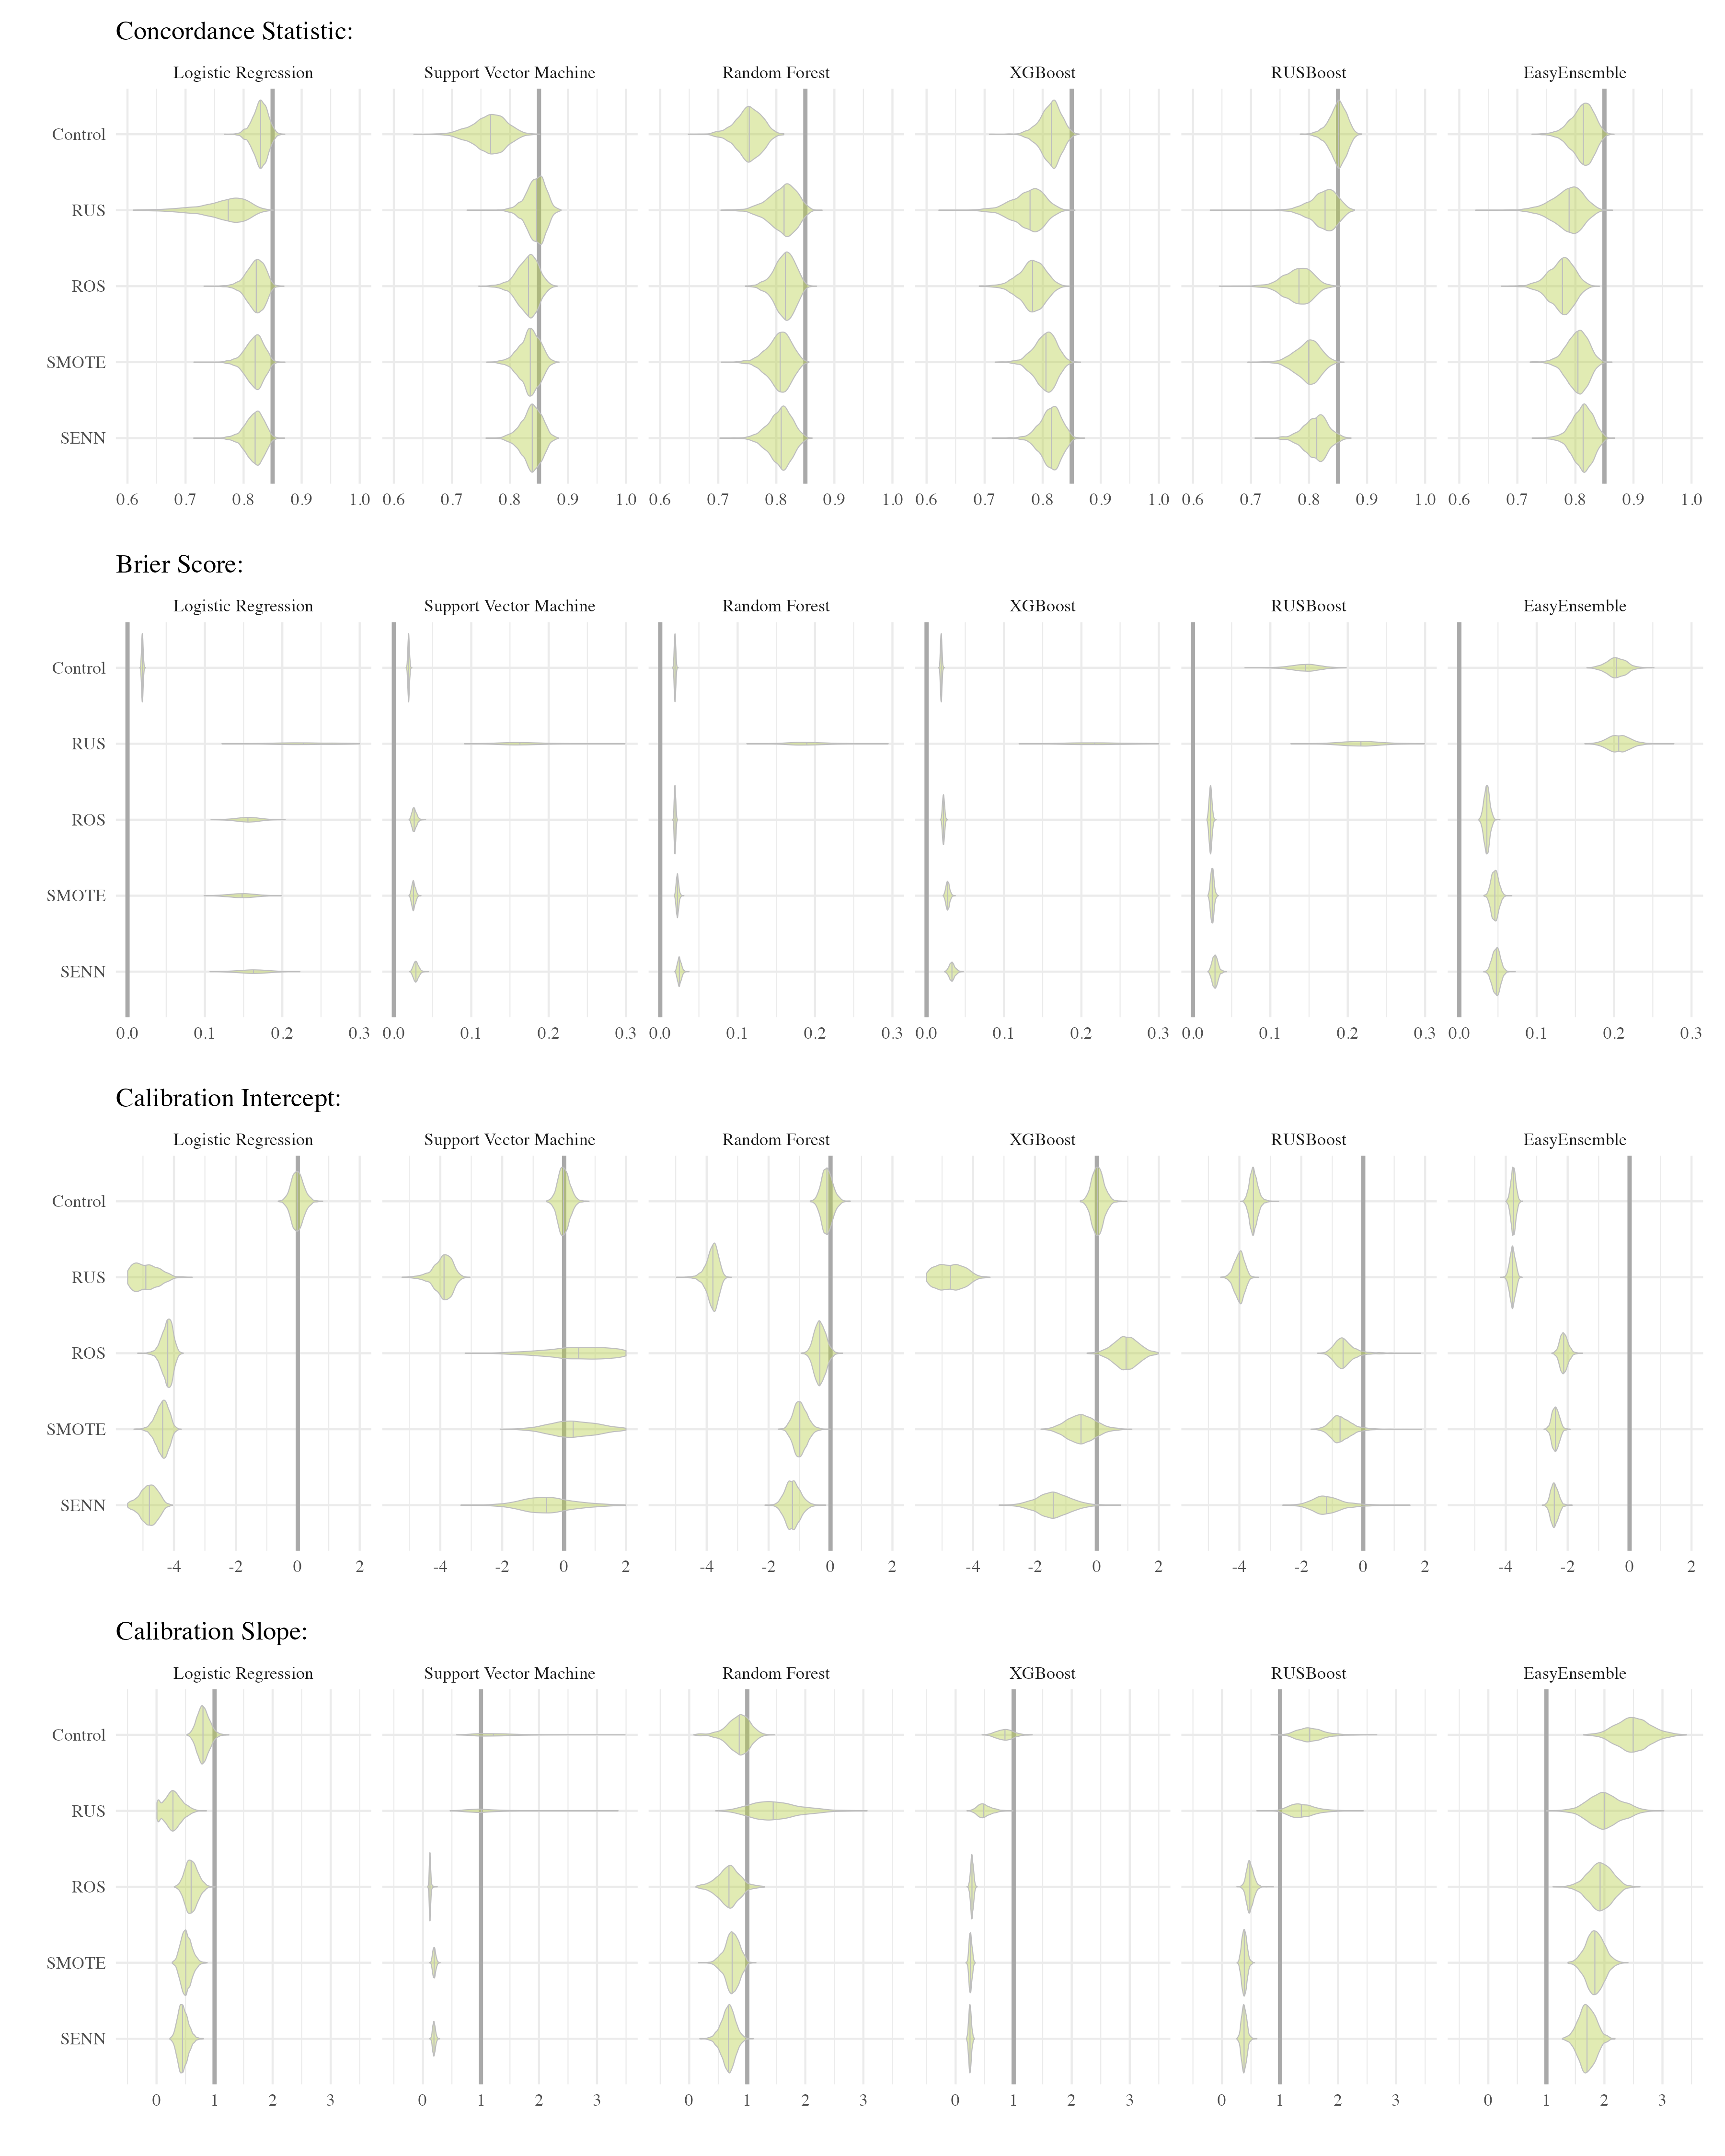
\includegraphics[width=0.7\linewidth]{./figures/performance_metrics_manuscript_sc12} 

}

\caption{Empirical performance metrics for each of 2000 simulation iterations in simulation scenario 12.  This simulation scenario is characterized by 16 predictors, half the required sample size (0.5N) and strongly imbalanced data (event fraction = 0.02). Empirical performance metrics were computed with raw predicted risks; no re-calibration. The target value highlighted for concordance statistic reflects the data-generating concordance statstic, 0.85. Imbalance corrections: RUS (random undersampling), ROS (random oversampling), SMOTE (synthetic majority oversampling), SENN (synthetic majority oversampling with Wilson's Edited Nearest Neighbors). \label{fig:violin_12}}\label{fig:unnamed-chunk-50}
\end{figure}

\begin{figure}

{\centering 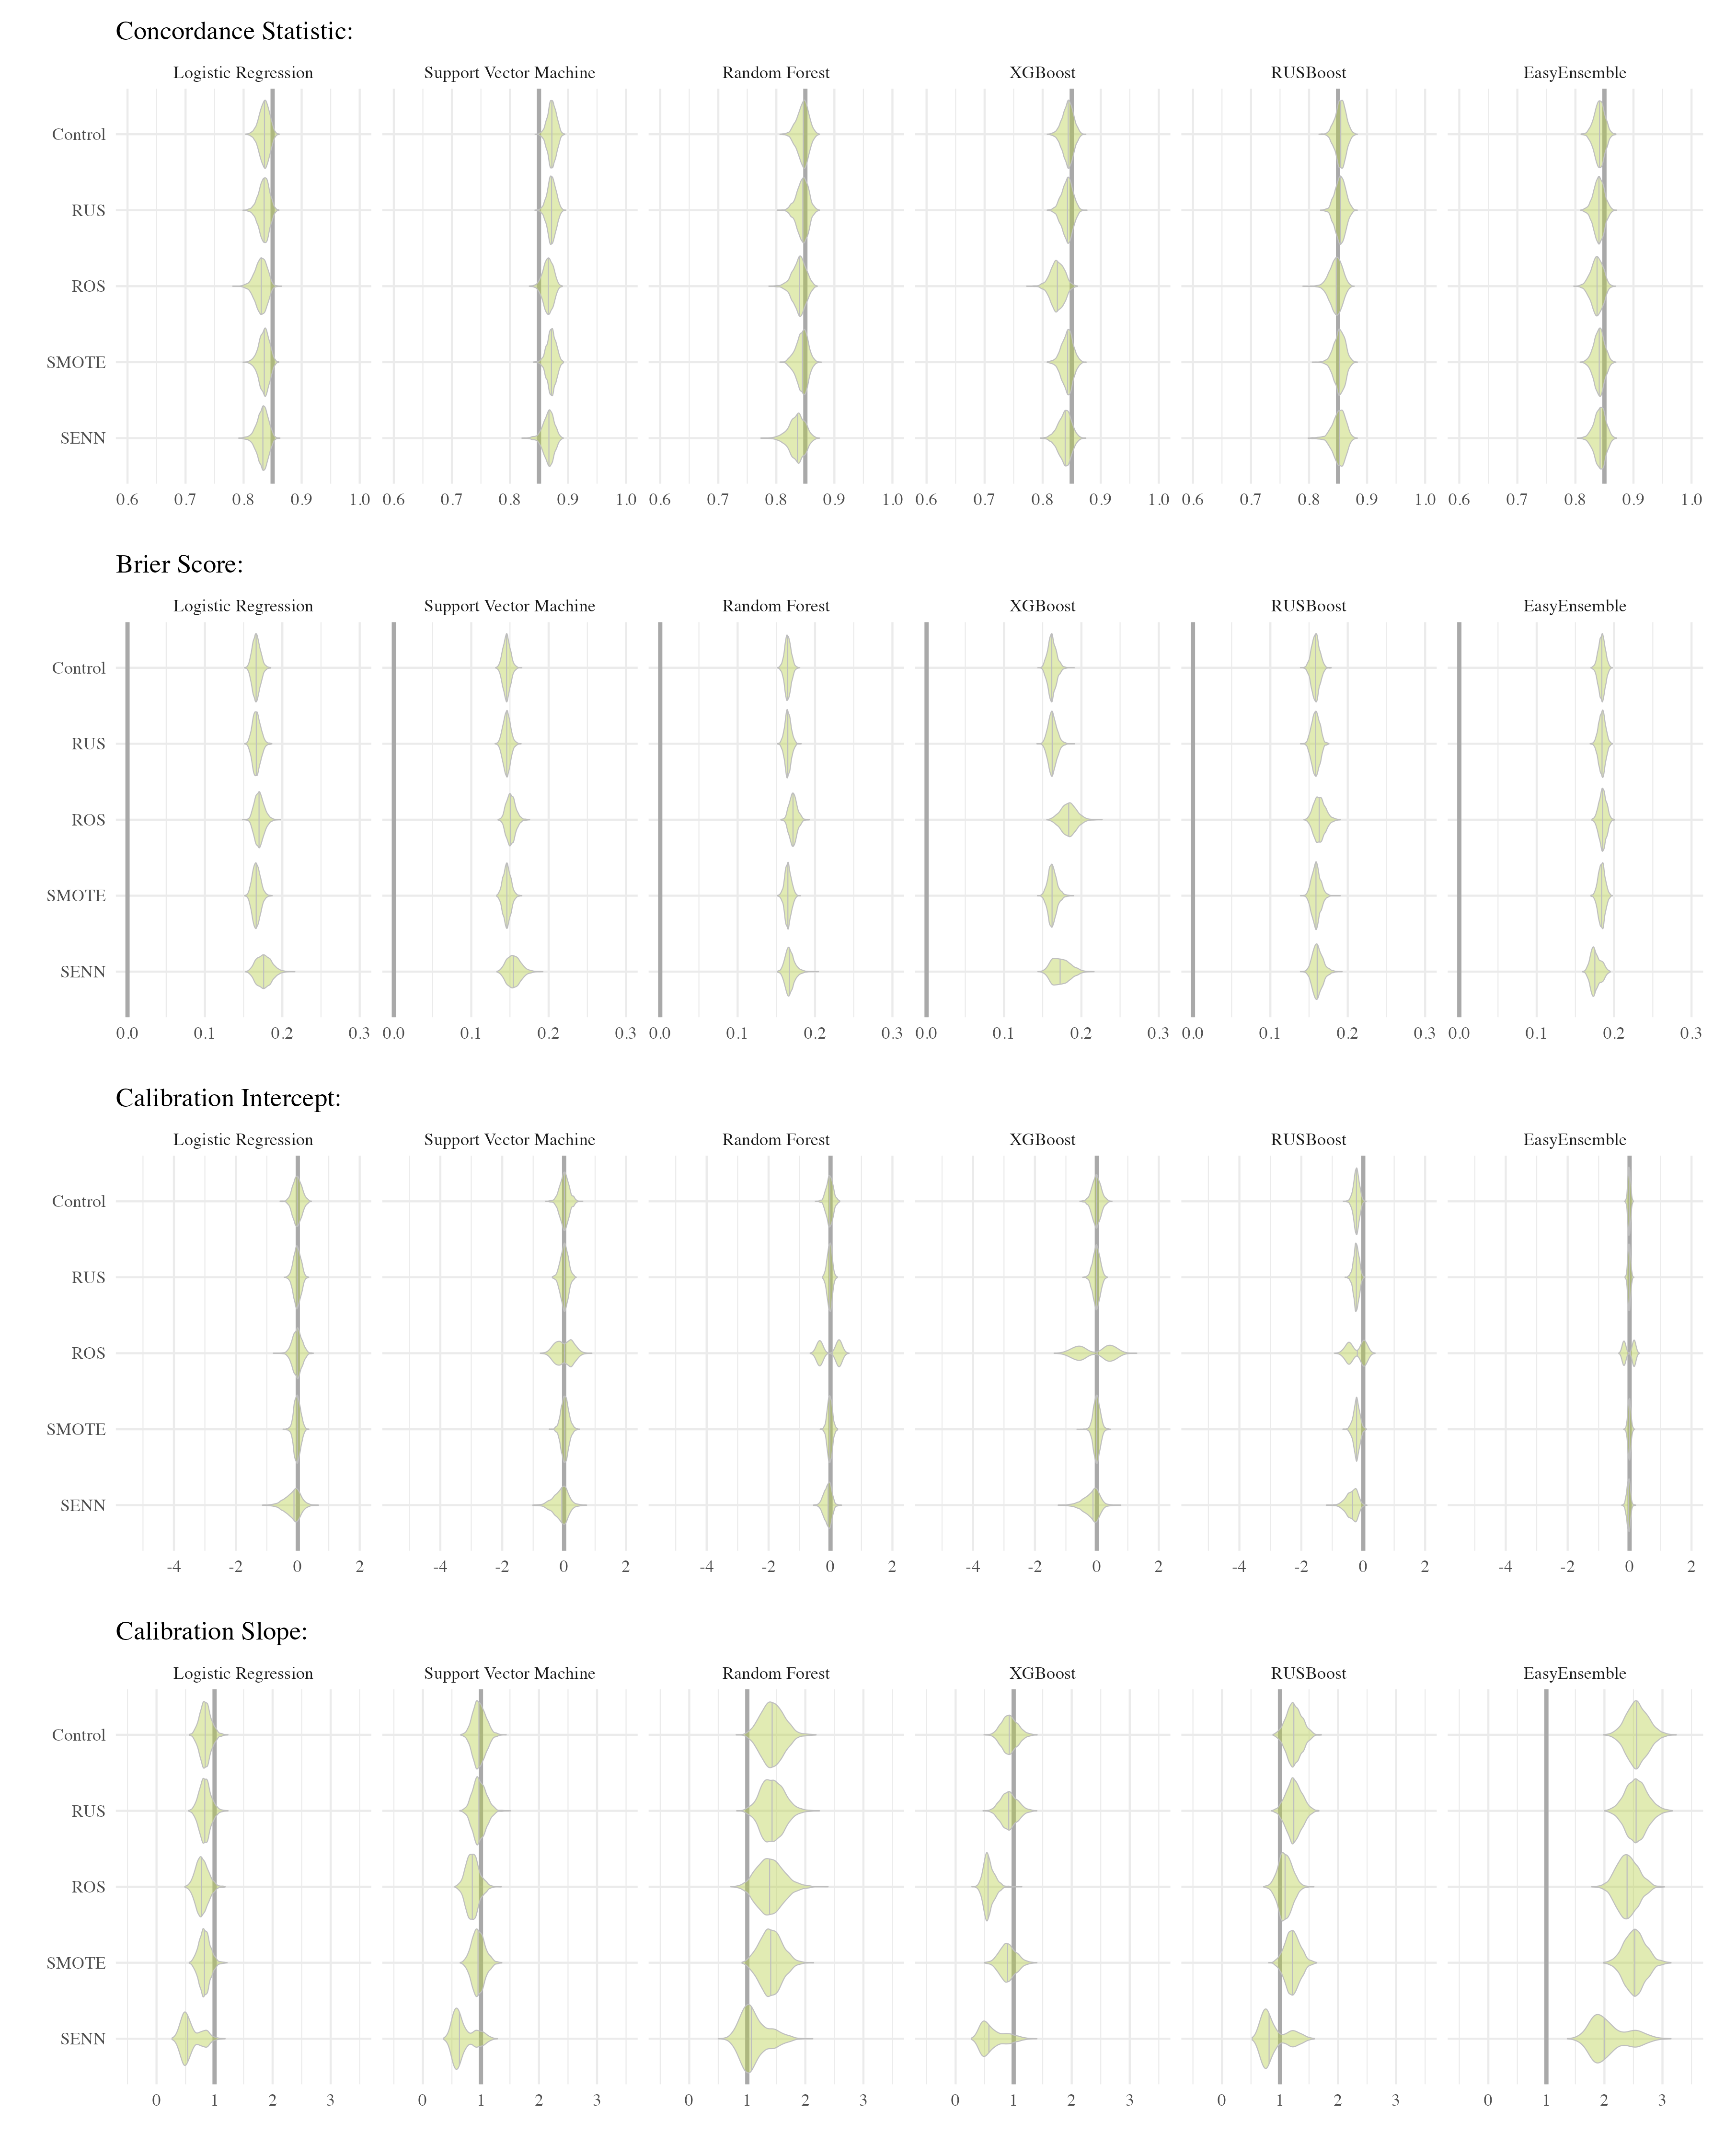
\includegraphics[width=0.7\linewidth]{./figures/performance_metrics_manuscript_sc13} 

}

\caption{Empirical performance metrics for each of 2000 simulation iterations in simulation scenario 13.  This simulation scenario is characterized by 16 predictors, minimum required sample size (N) and class balanced data (event fraction = 0.5). Empirical performance metrics were computed with raw predicted risks; no re-calibration. The target value highlighted for concordance statistic reflects the data-generating concordance statstic, 0.85. Imbalance corrections: RUS (random undersampling), ROS (random oversampling), SMOTE (synthetic majority oversampling), SENN (synthetic majority oversampling with Wilson's Edited Nearest Neighbors). \label{fig:violin_13}}\label{fig:unnamed-chunk-51}
\end{figure}

\begin{figure}

{\centering 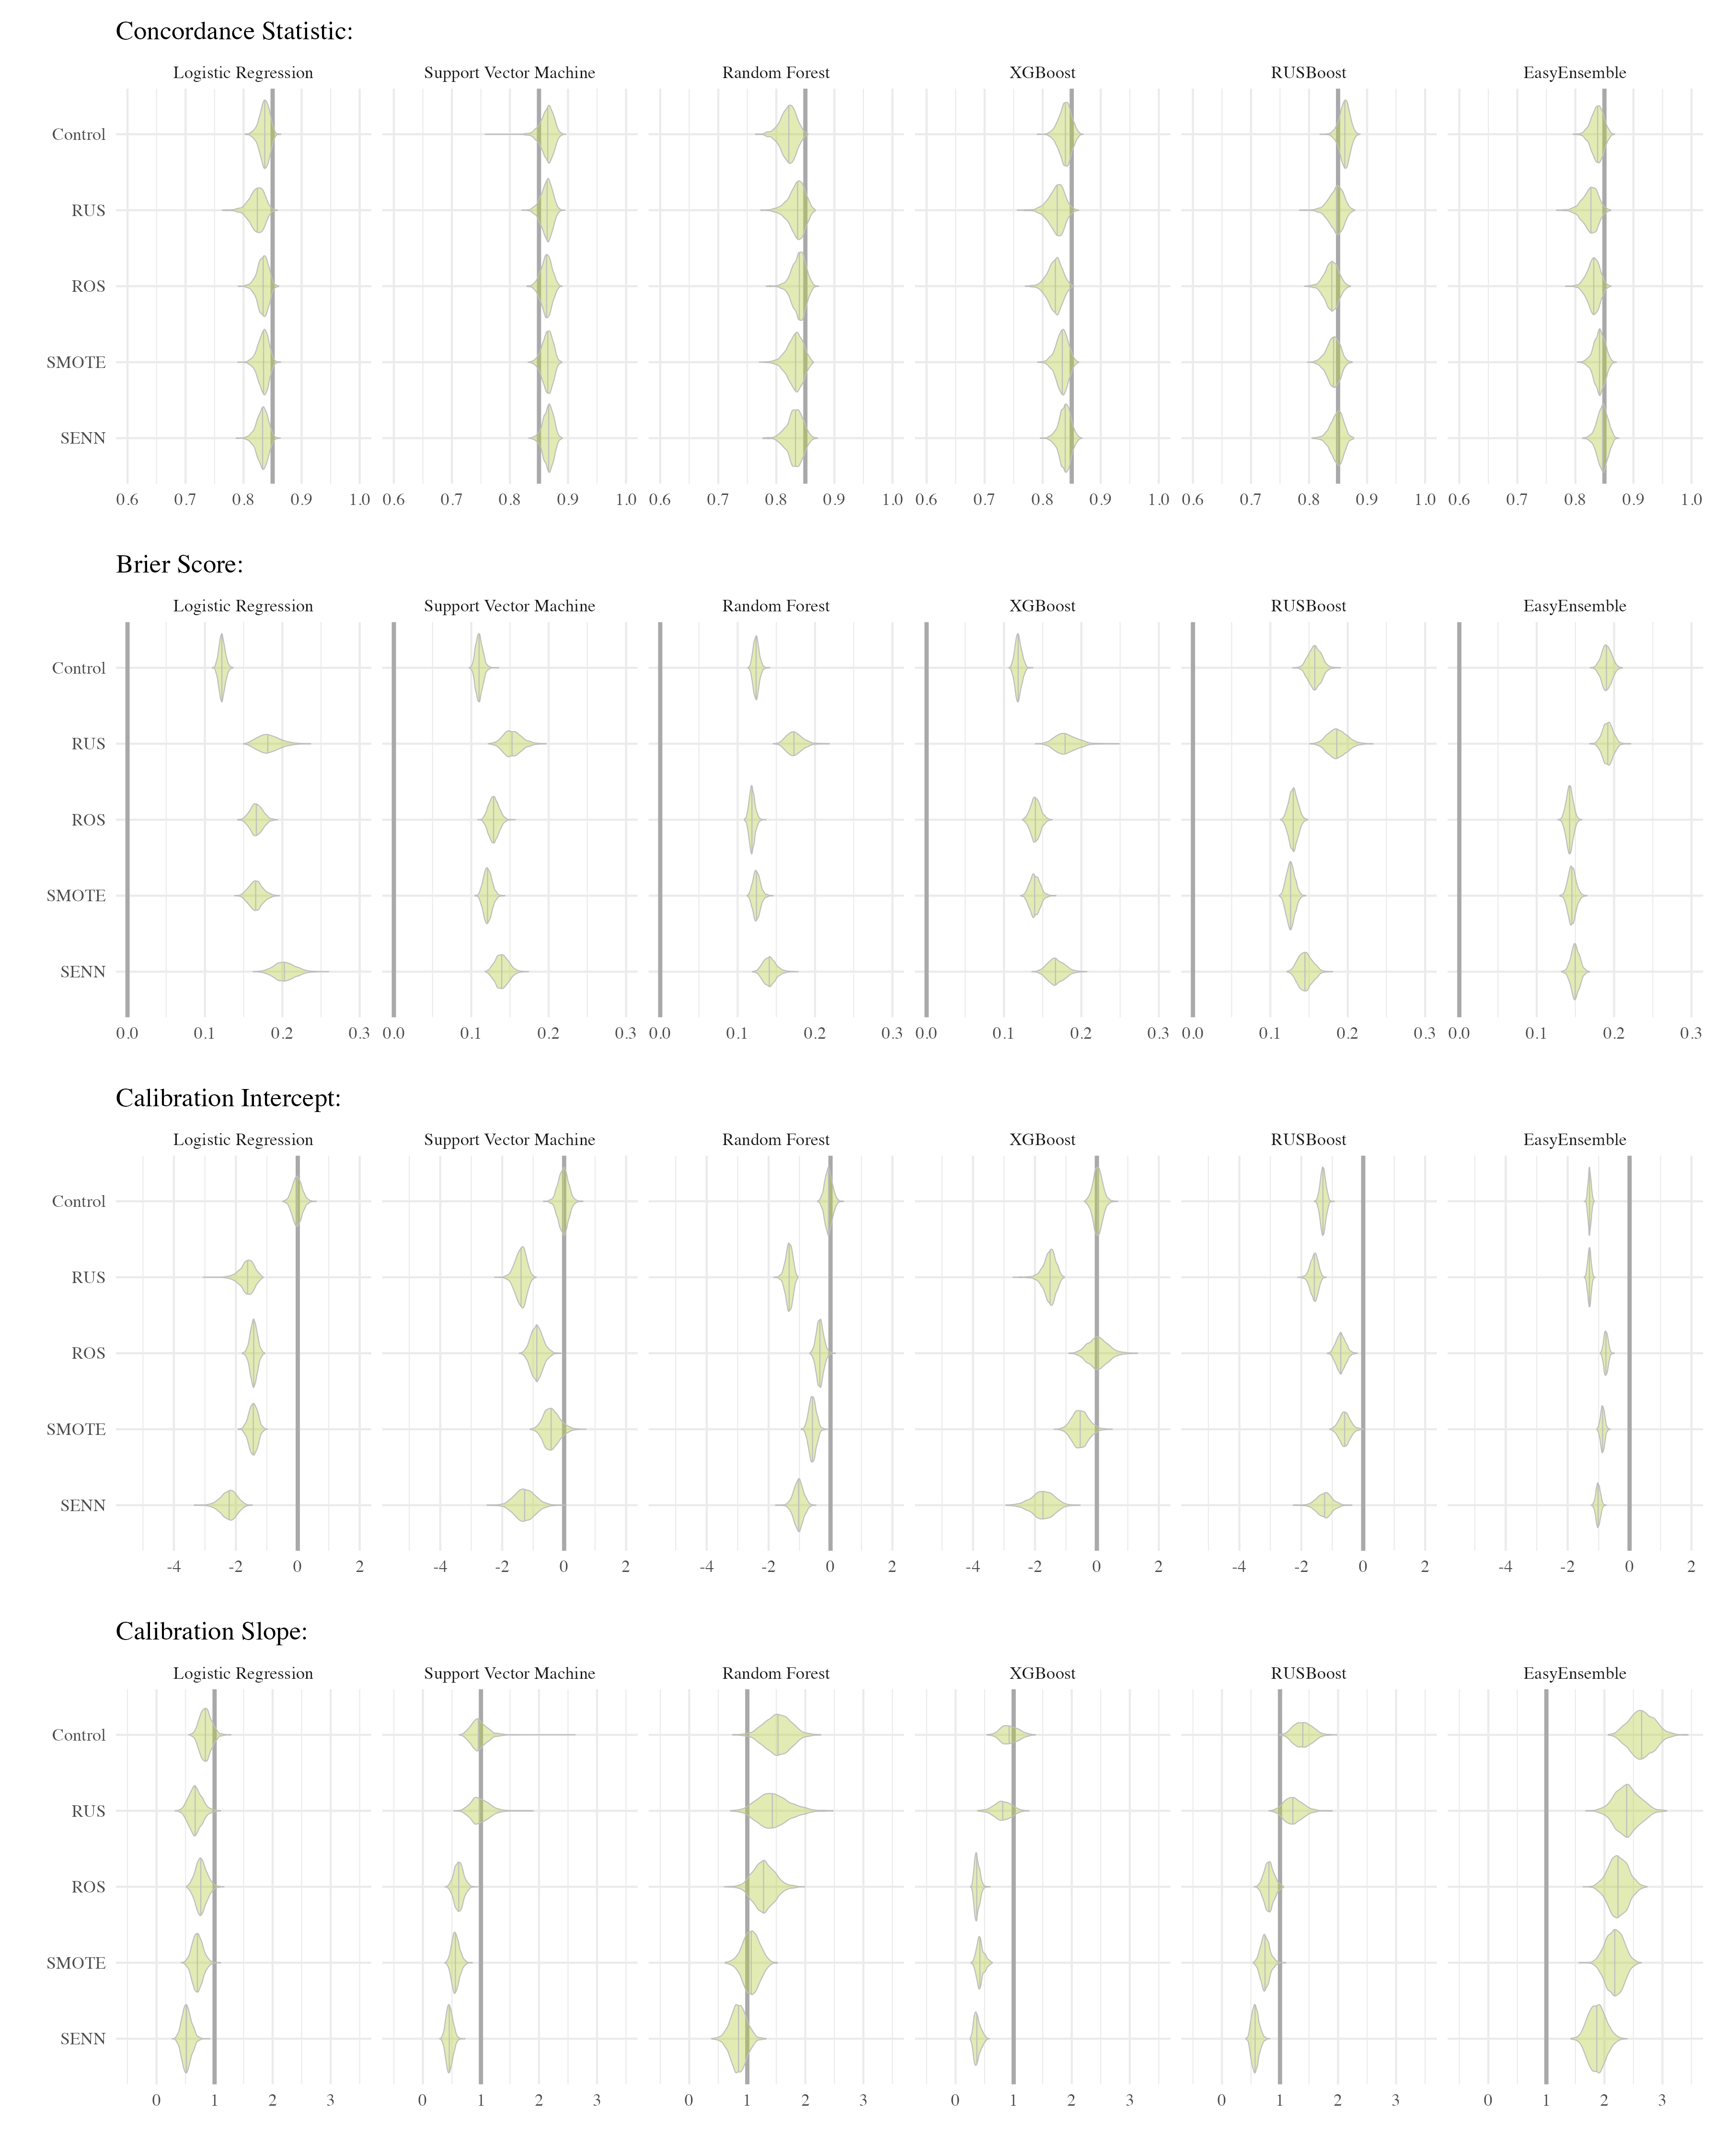
\includegraphics[width=0.7\linewidth]{./figures/performance_metrics_manuscript_sc14} 

}

\caption{Empirical performance metrics for each of 2000 simulation iterations in simulation scenario 14.  This simulation scenario is characterized by 16 predictors, minimum required sample size (N) and moderately imbalanced data (event fraction = 0.2). Empirical performance metrics were computed with raw predicted risks; no re-calibration. The target value highlighted for concordance statistic reflects the data-generating concordance statstic, 0.85. Imbalance corrections: RUS (random undersampling), ROS (random oversampling), SMOTE (synthetic majority oversampling), SENN (synthetic majority oversampling with Wilson's Edited Nearest Neighbors). \label{fig:violin_14}}\label{fig:unnamed-chunk-52}
\end{figure}

\begin{figure}

{\centering 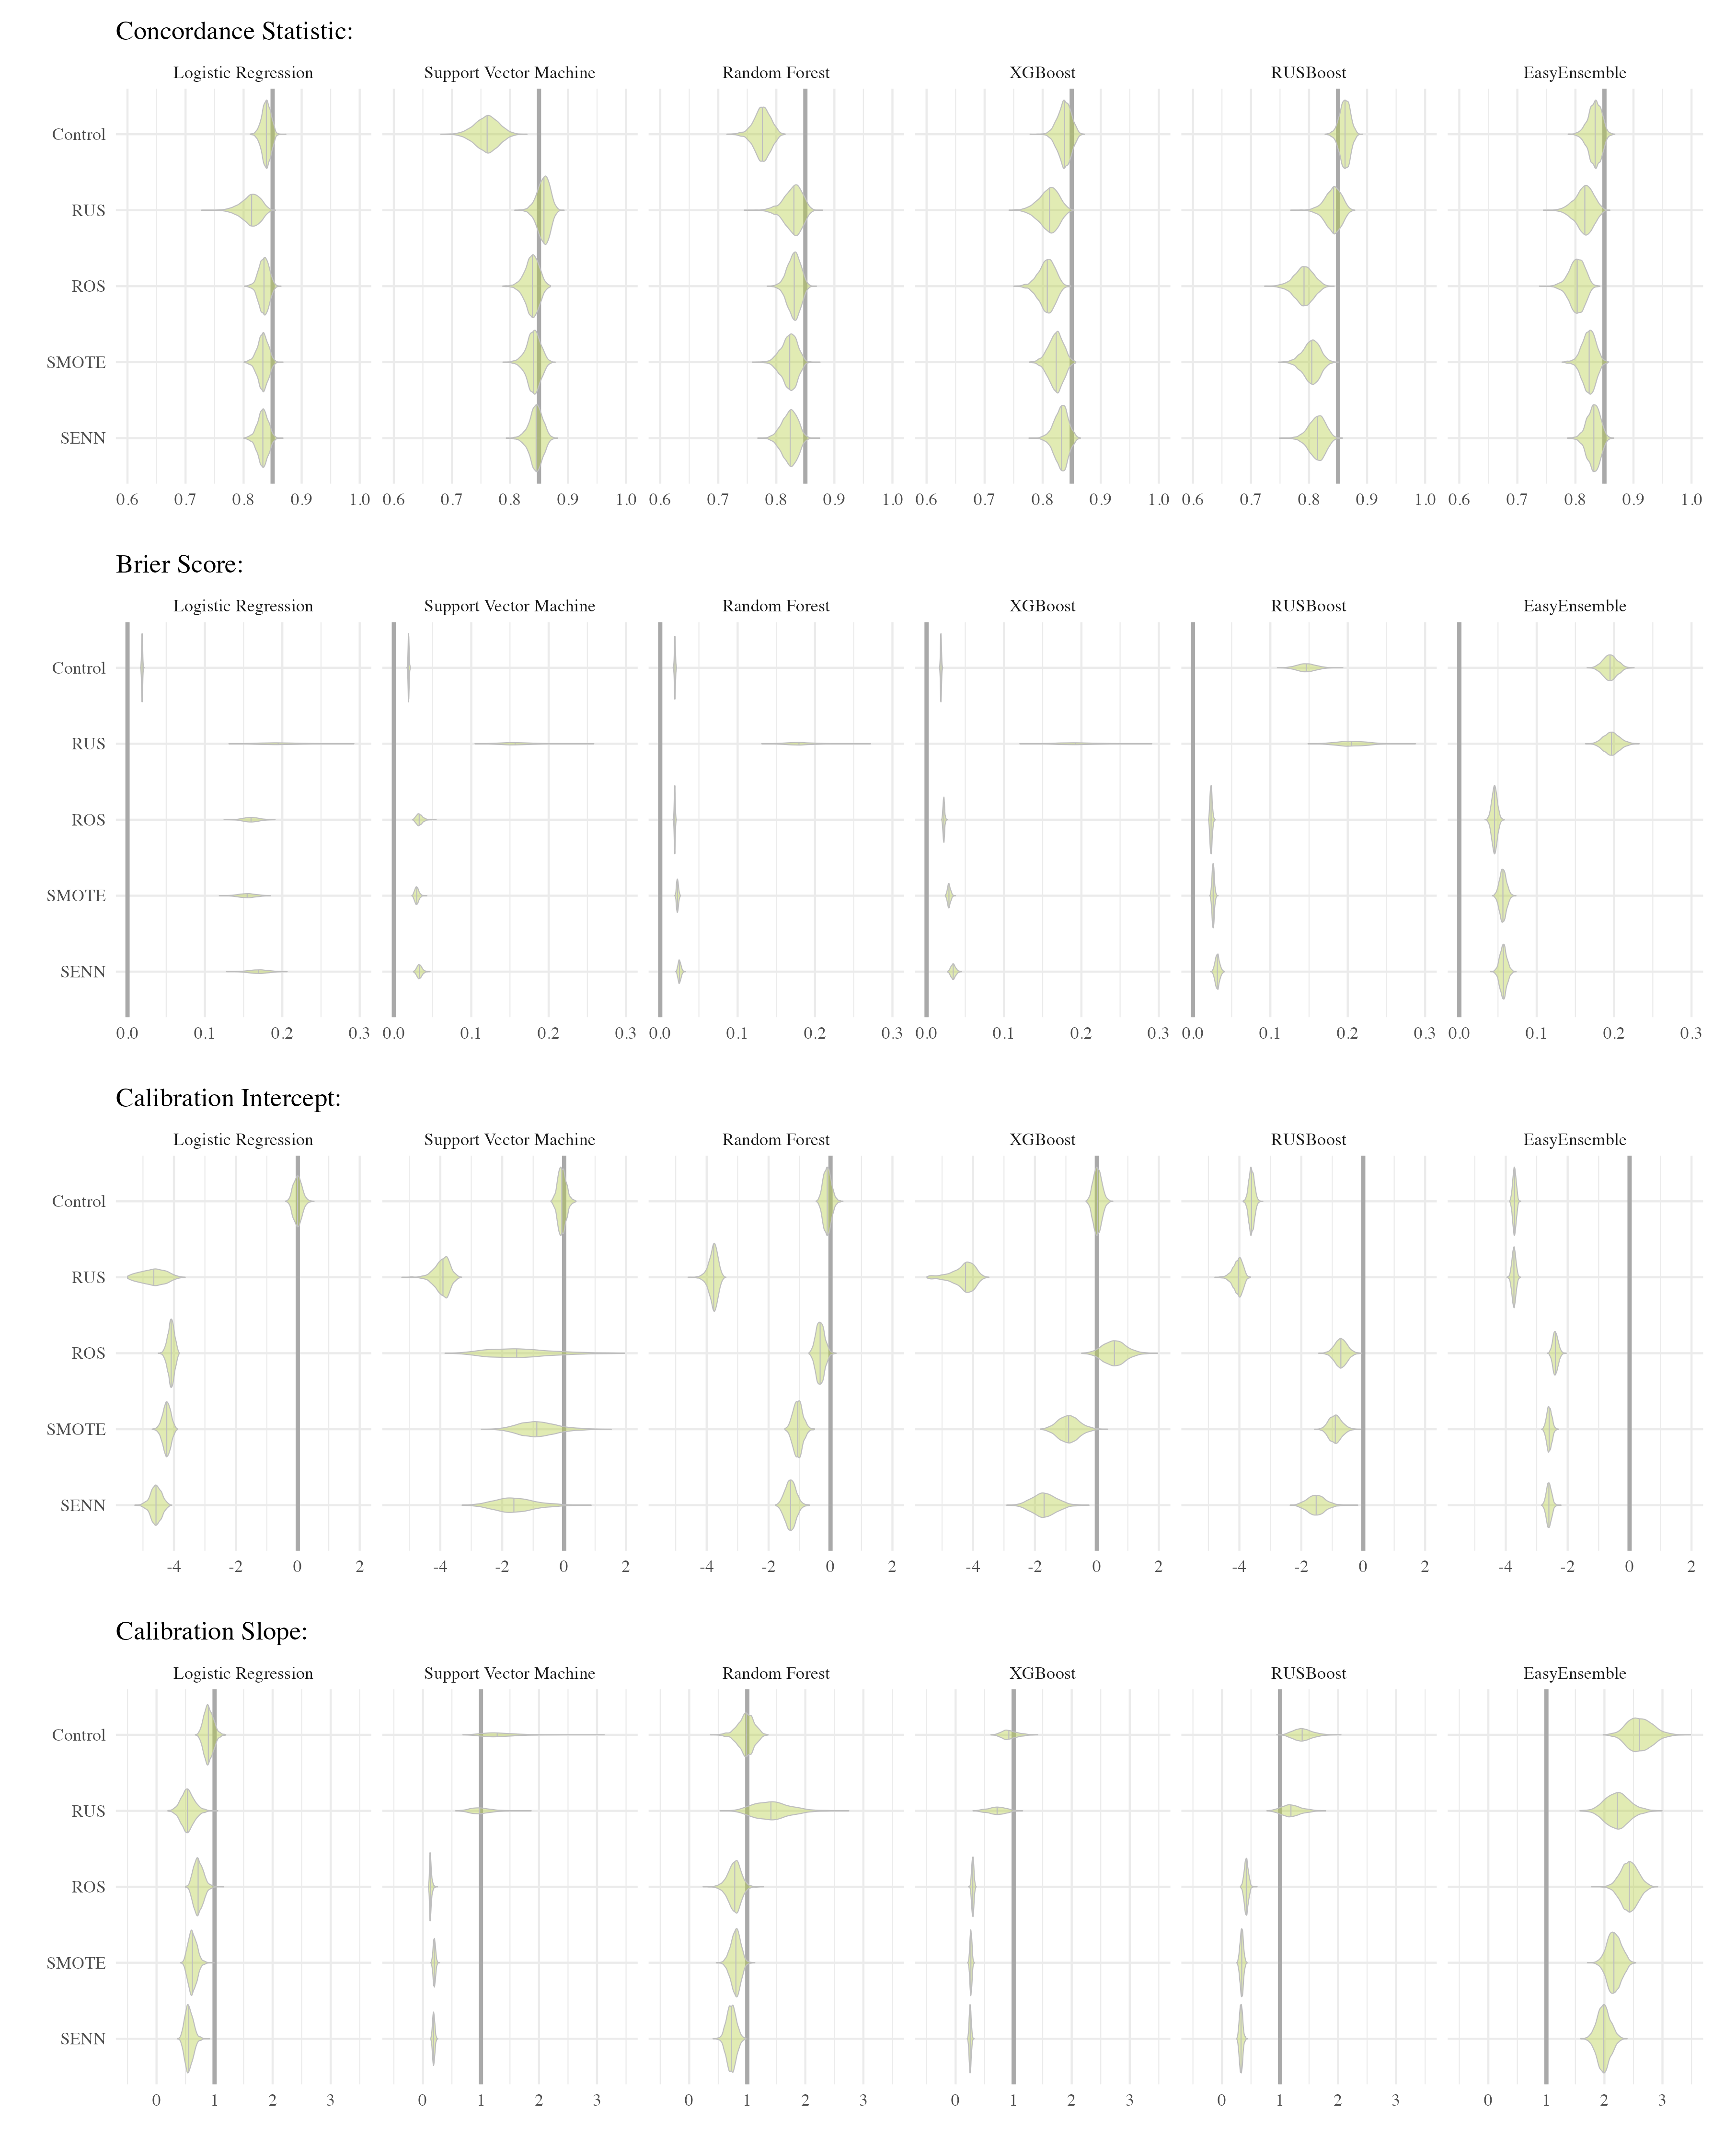
\includegraphics[width=0.7\linewidth]{./figures/performance_metrics_manuscript_sc15} 

}

\caption{Empirical performance metrics for each of 2000 simulation iterations in simulation scenario 15.  This simulation scenario is characterized by 16 predictors, minimum required sample size (N) and strongly imbalanced data (event fraction = 0.02).  Empirical performance metrics were computed with raw predicted risks; no re-calibration. The target value highlighted for concordance statistic reflects the data-generating concordance statstic, 0.85. Imbalance corrections: RUS (random undersampling), ROS (random oversampling), SMOTE (synthetic majority oversampling), SENN (synthetic majority oversampling with Wilson's Edited Nearest Neighbors). \label{fig:violin_15}}\label{fig:unnamed-chunk-53}
\end{figure}

\begin{figure}

{\centering 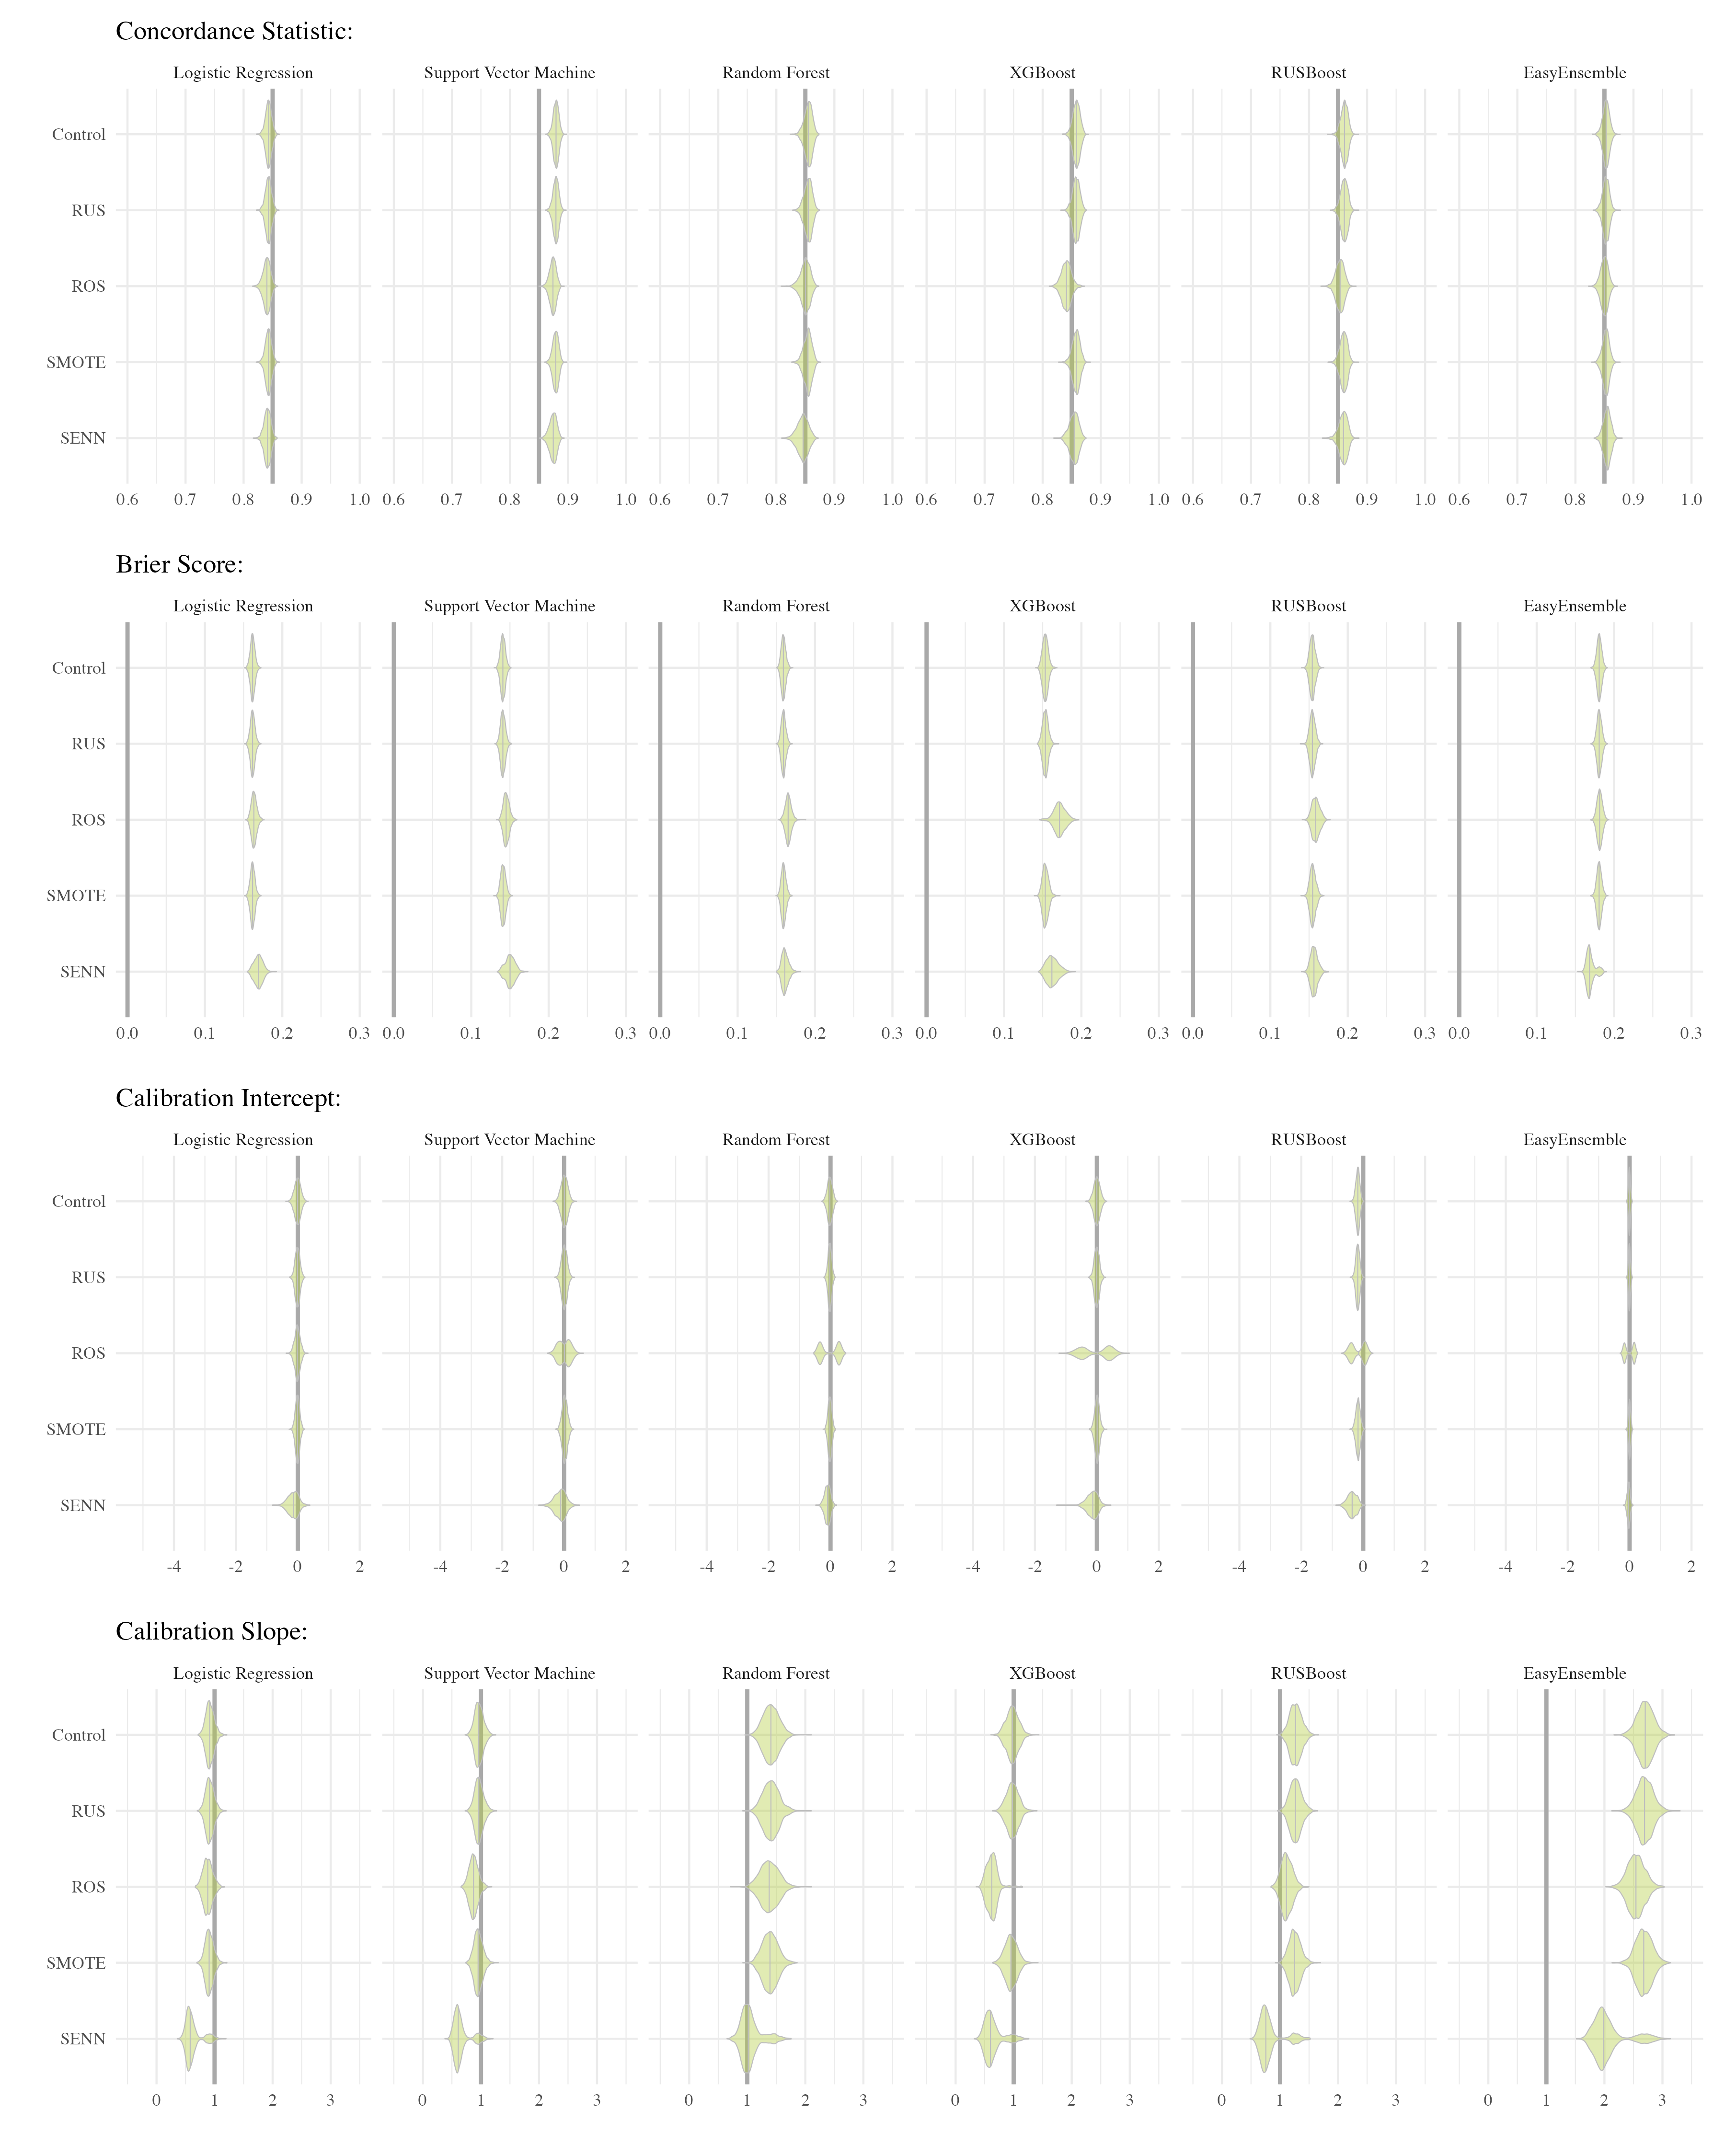
\includegraphics[width=0.7\linewidth]{./figures/performance_metrics_manuscript_sc16} 

}

\caption{Empirical performance metrics for each of 2000 simulation iterations in simulation scenario 16.  This simulation scenario is characterized by 16 predictors, double the required sample size (2N) and class balanced data (event fraction = 0.5). Empirical performance metrics were computed with raw predicted risks; no re-calibration. The target value highlighted for concordance statistic reflects the data-generating concordance statstic, 0.85. Imbalance corrections: RUS (random undersampling), ROS (random oversampling), SMOTE (synthetic majority oversampling), SENN (synthetic majority oversampling with Wilson's Edited Nearest Neighbors). \label{fig:violin_16}}\label{fig:unnamed-chunk-54}
\end{figure}

\begin{figure}

{\centering 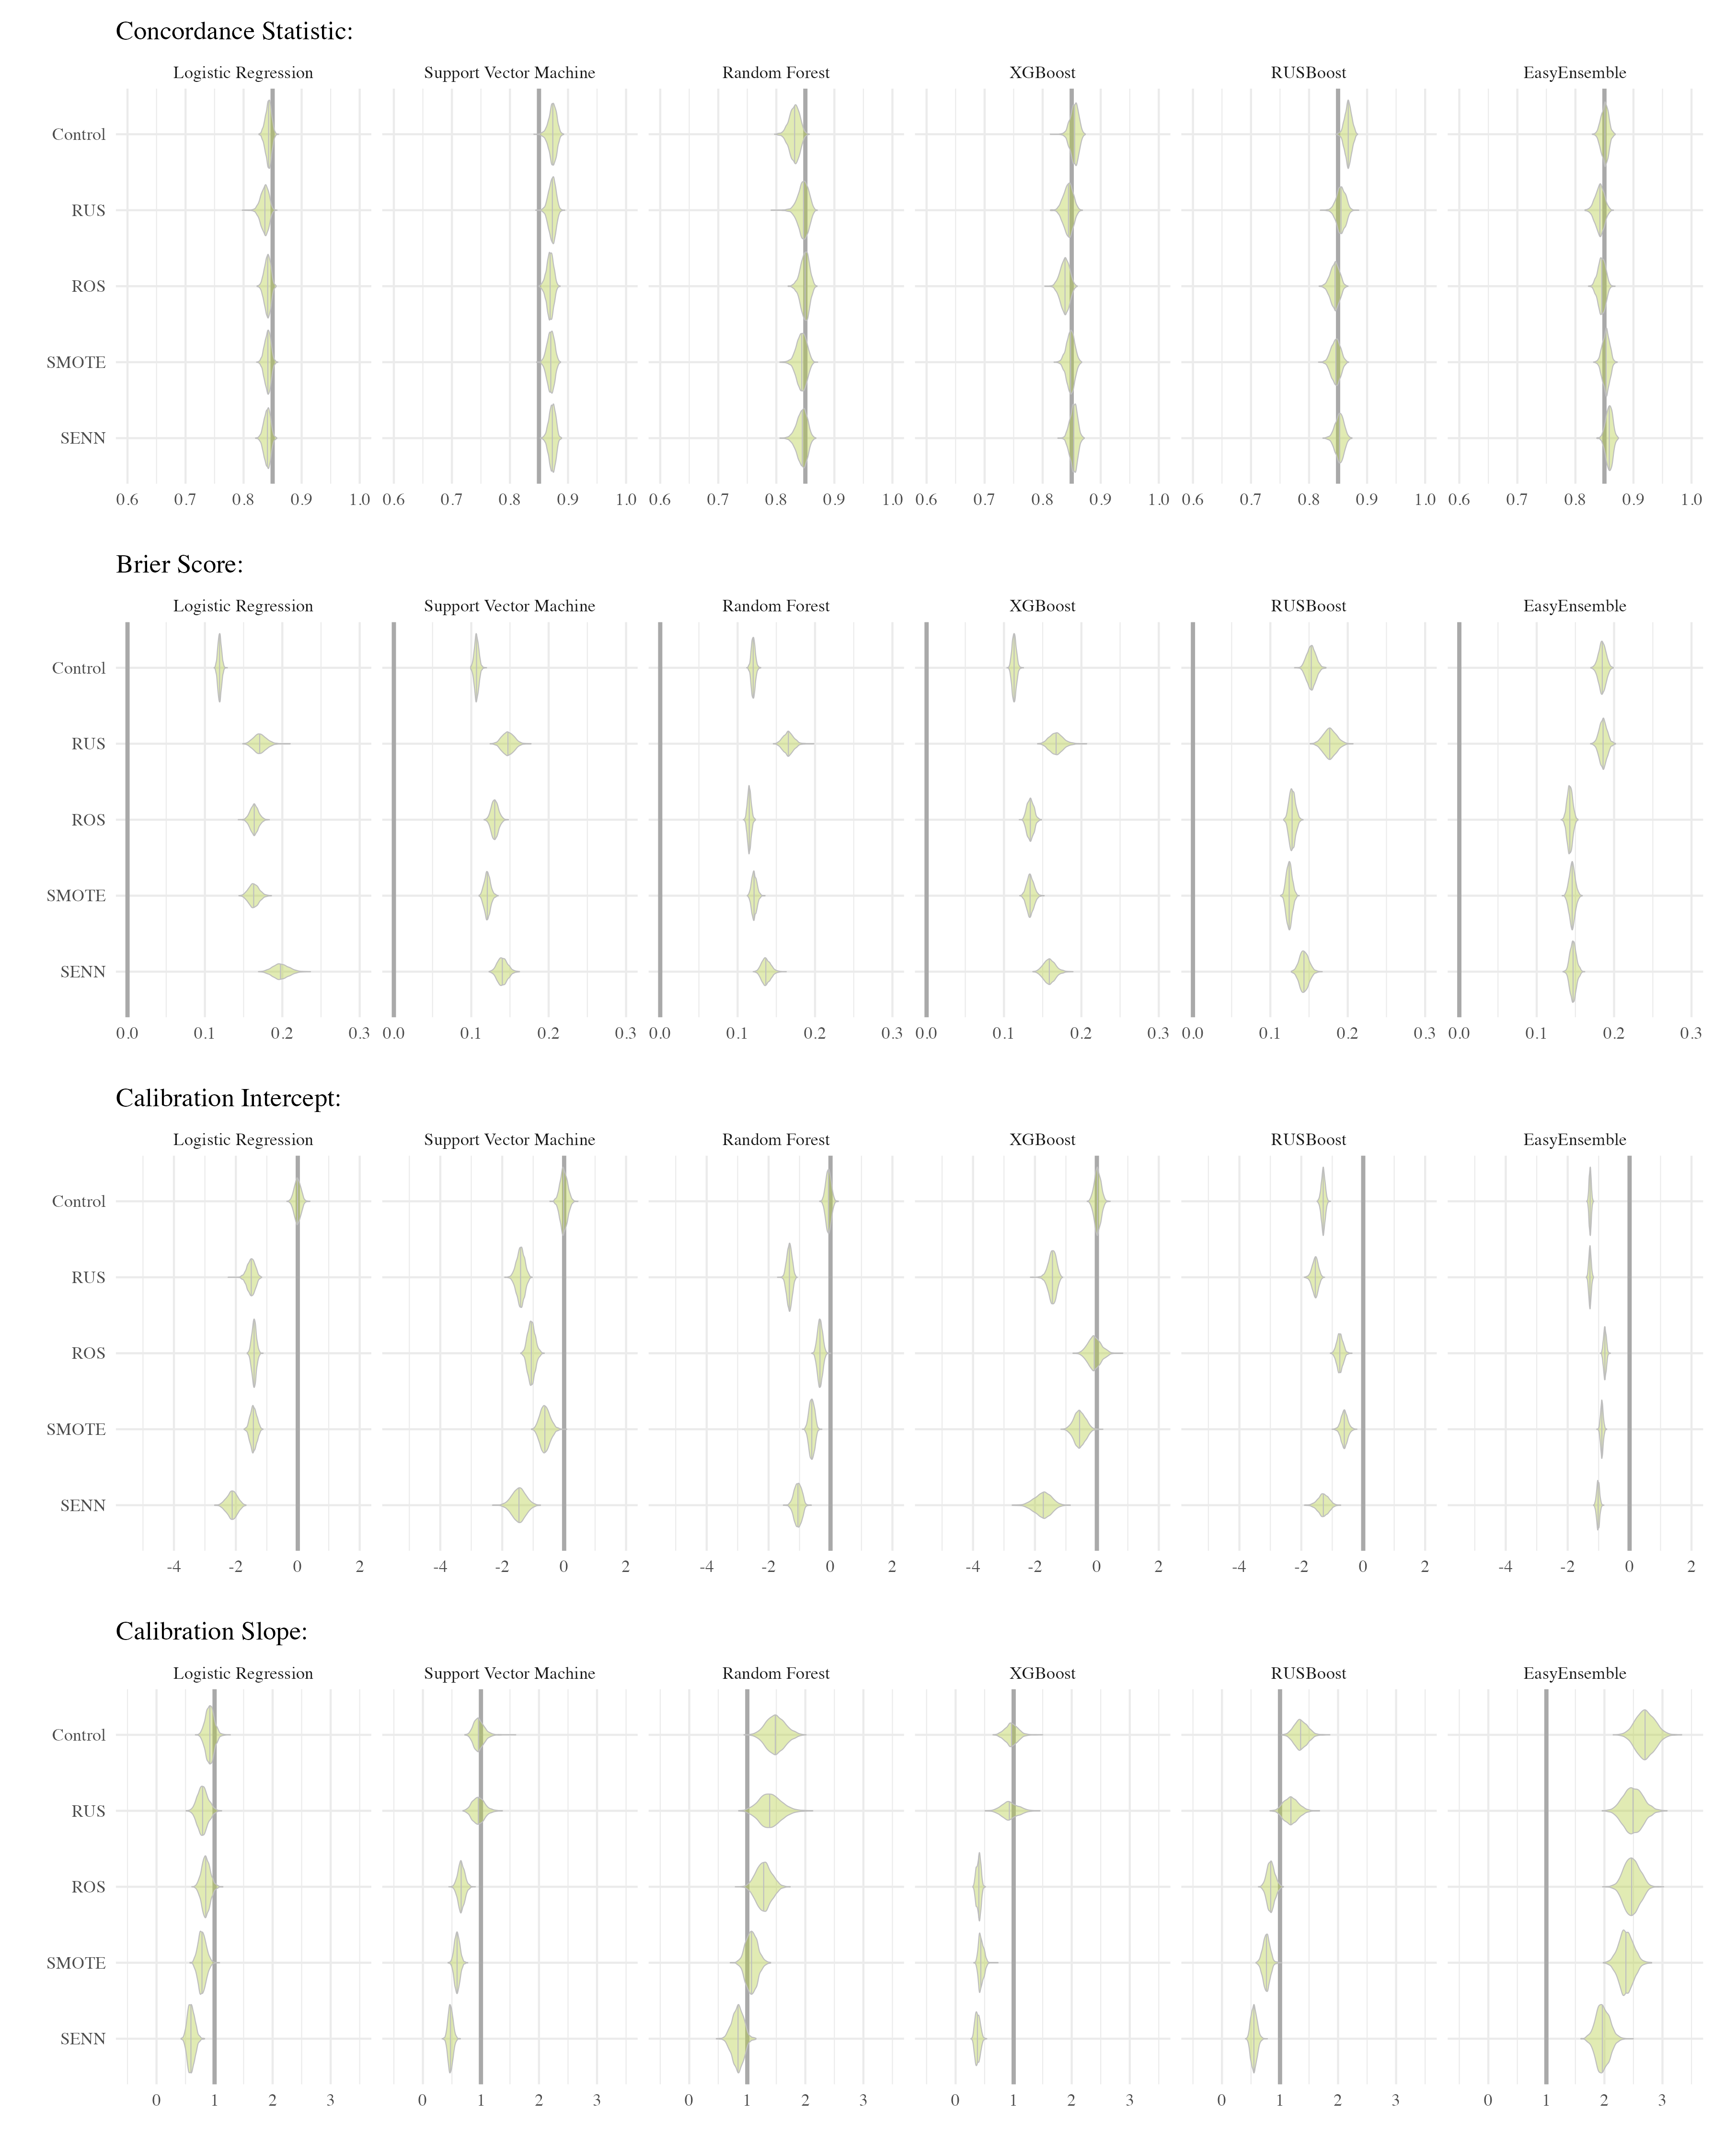
\includegraphics[width=0.7\linewidth]{./figures/performance_metrics_manuscript_sc17} 

}

\caption{Empirical performance metrics for each of 2000 simulation iterations in simulation scenario 17.  This simulation scenario is characterized by 16 predictors, double the required sample size (2N) and moderately imbalanced data (event fraction = 0.2). Empirical performance metrics were computed with raw predicted risks; no re-calibration. The target value highlighted for concordance statistic reflects the data-generating concordance statstic, 0.85. Imbalance corrections: RUS (random undersampling), ROS (random oversampling), SMOTE (synthetic majority oversampling), SENN (synthetic majority oversampling with Wilson's Edited Nearest Neighbors). \label{fig:violin_17}}\label{fig:unnamed-chunk-55}
\end{figure}
\clearpage
\begin{figure}

{\centering 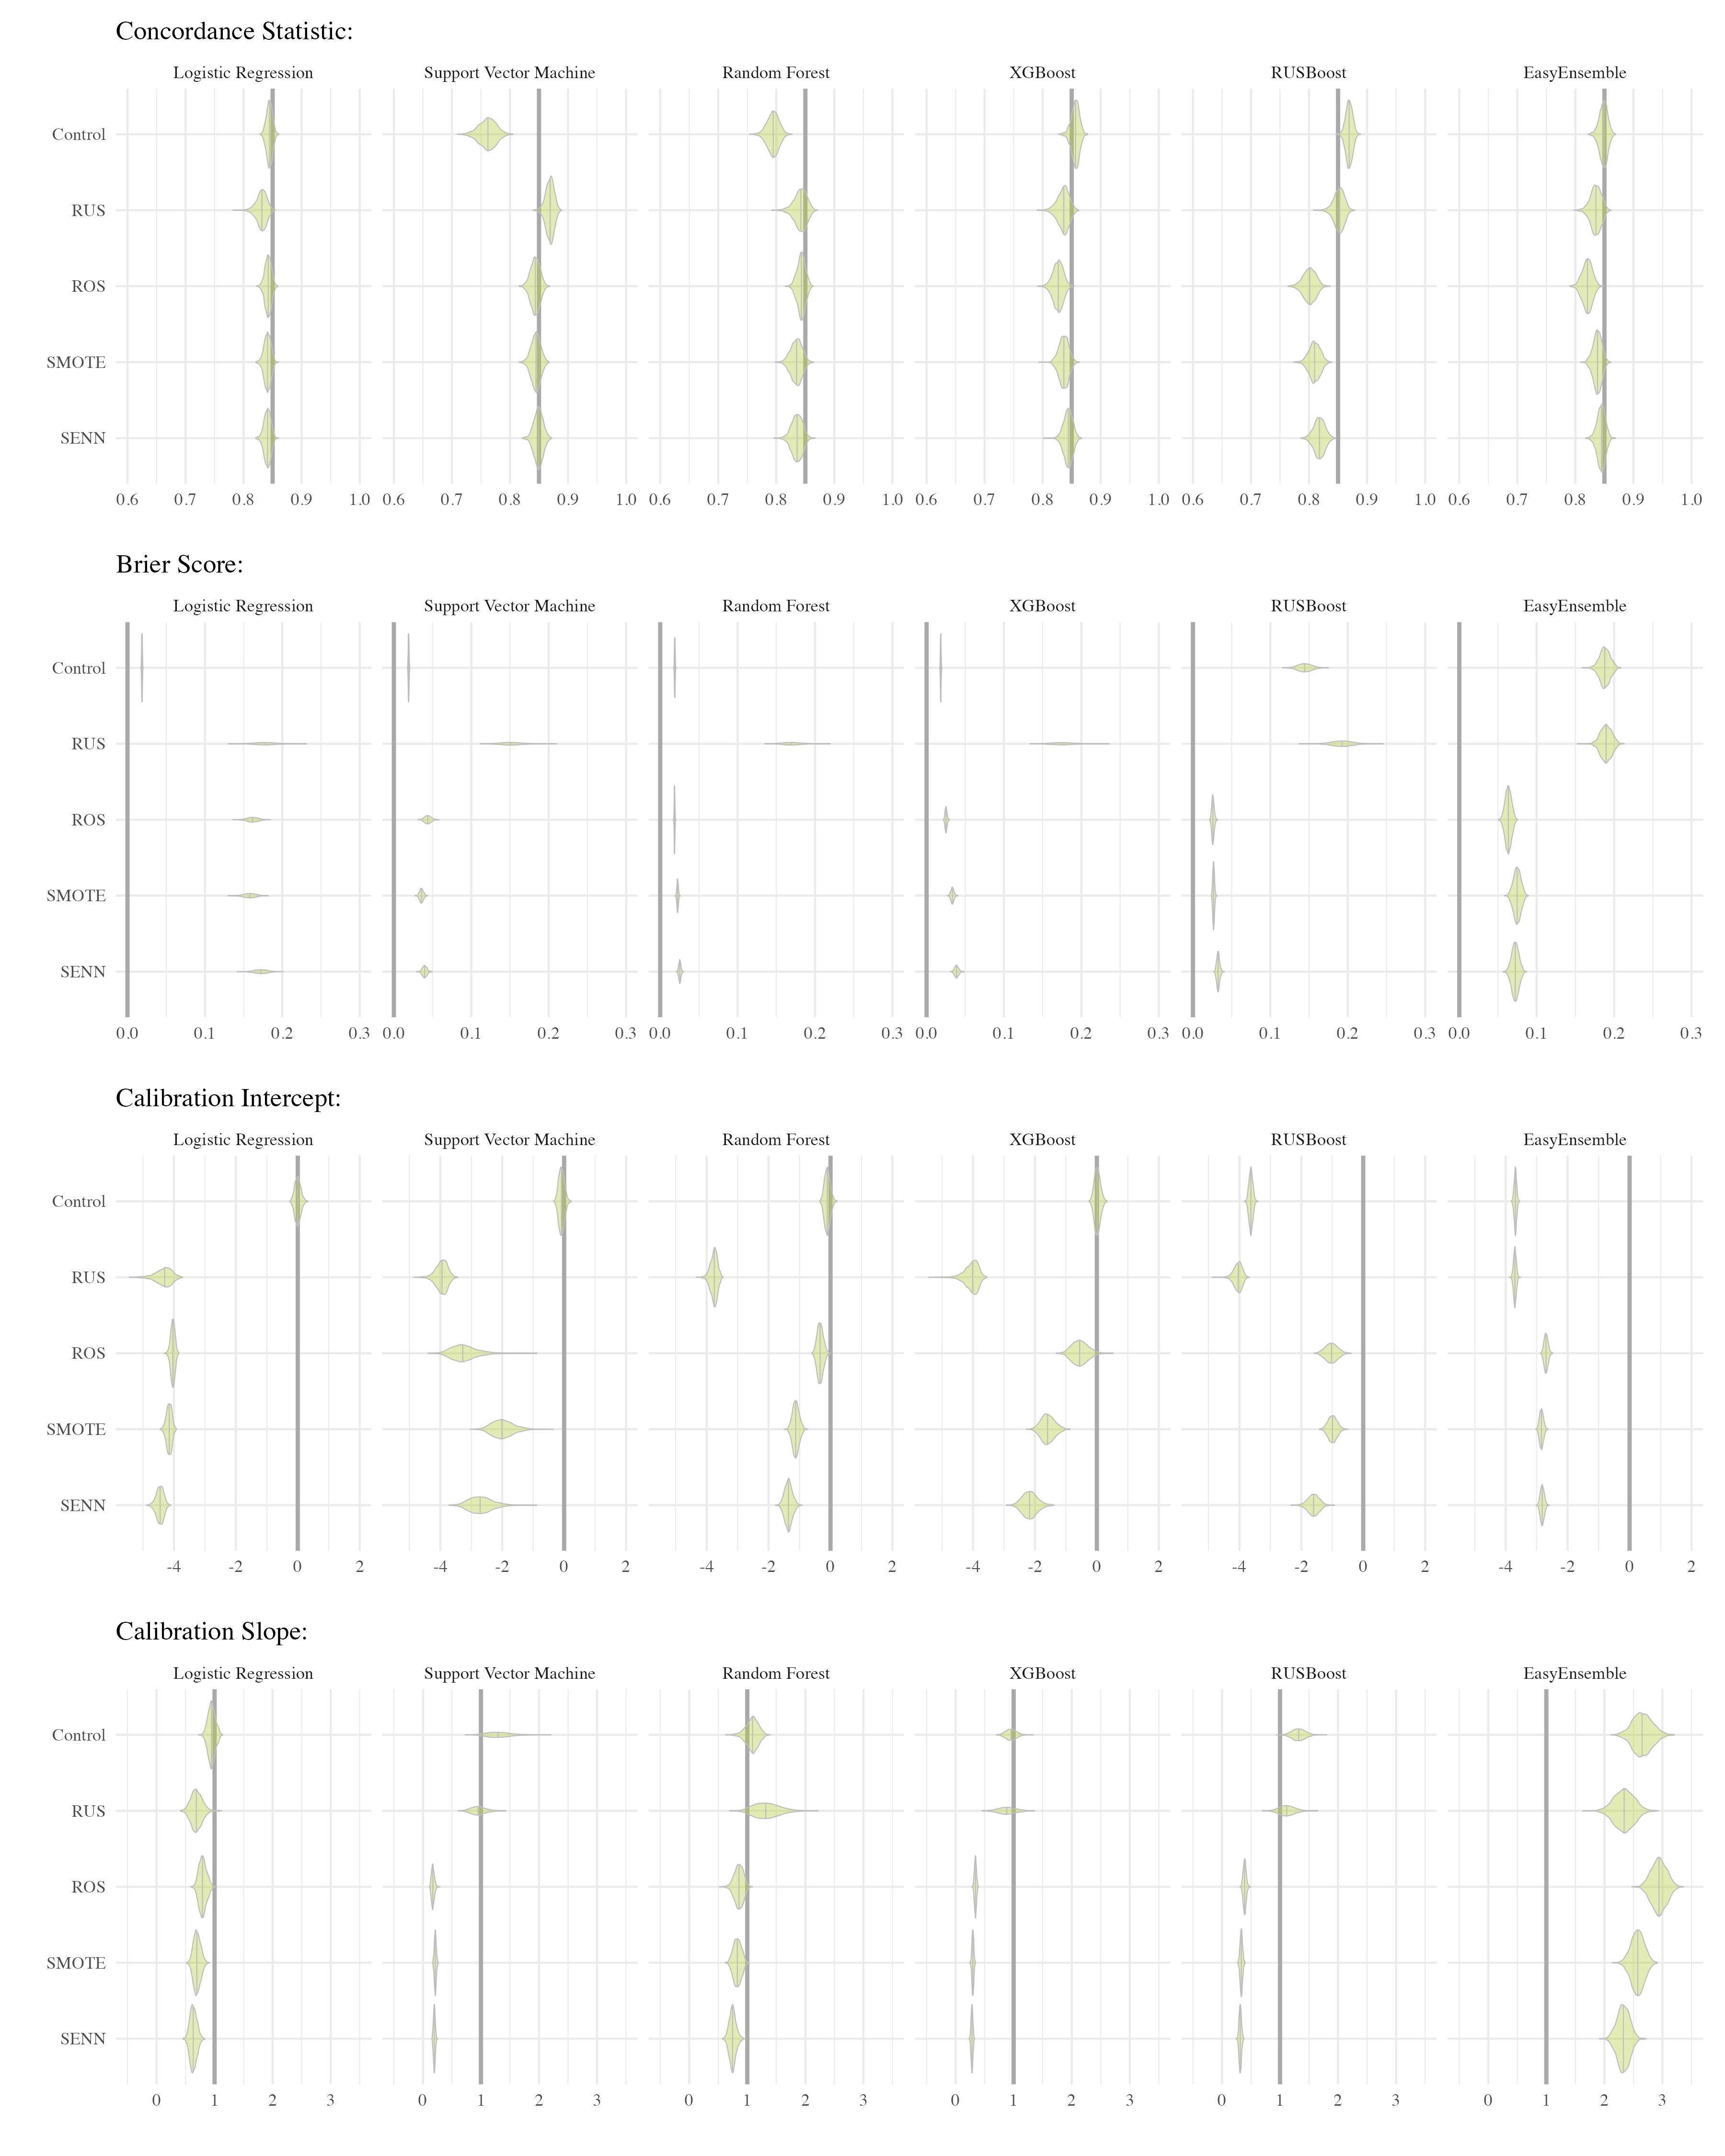
\includegraphics[width=0.7\linewidth]{./figures/performance_metrics_manuscript_sc18} 

}

\caption{Empirical performance metrics for each of 2000 simulation iterations in simulation scenario 18.  This simulation scenario is characterized by 16 predictors, double the required sample size (2N) and strongly imbalanced data (event fraction = 0.02). Empirical performance metrics were computed with raw predicted risks; no re-calibration. The target value highlighted for concordance statistic reflects the data-generating concordance statstic, 0.85. Imbalance corrections: RUS (random undersampling), ROS (random oversampling), SMOTE (synthetic majority oversampling), SENN (synthetic majority oversampling with Wilson's Edited Nearest Neighbors).\label{fig:violin_18}}\label{fig:unnamed-chunk-56}
\end{figure}

\newpage

\hypertarget{violin-plots-after-re-calibration}{%
\subsubsection{\texorpdfstring{Violin Plots (after re-calibration)\\
}{Violin Plots (after re-calibration) }}\label{violin-plots-after-re-calibration}}

\hfill\break

\begin{figure}[h]

{\centering 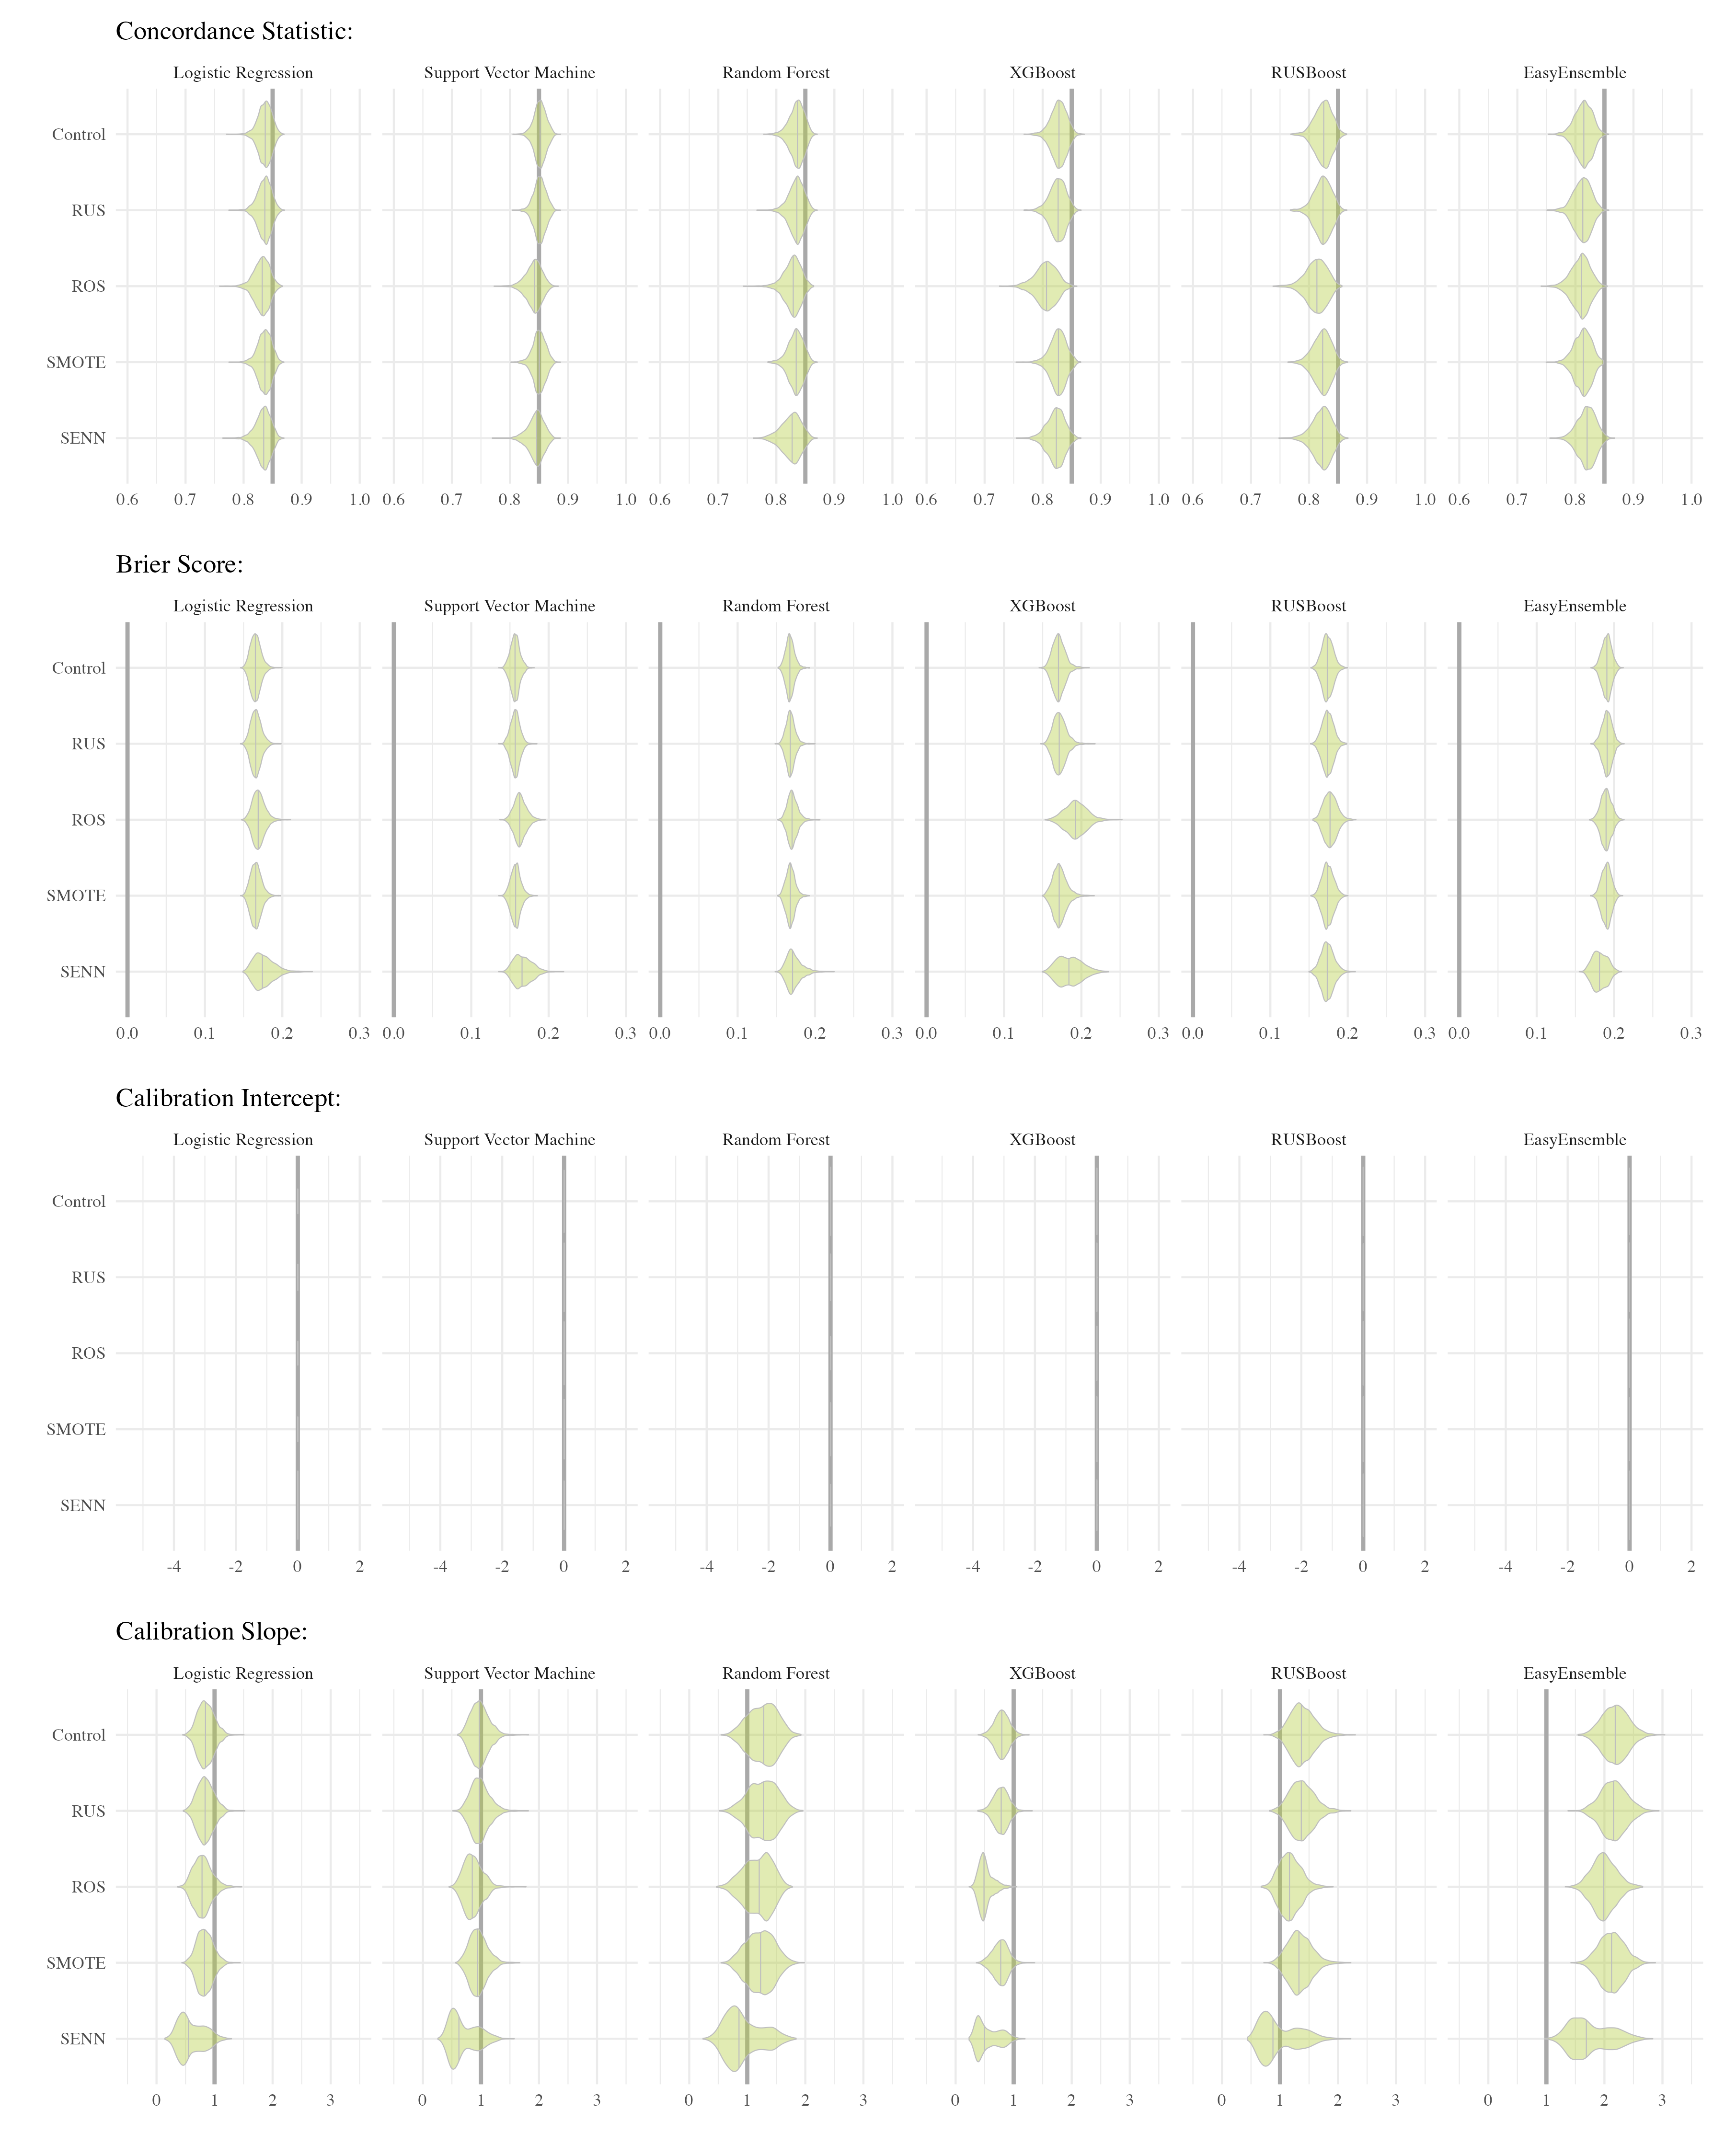
\includegraphics[width=0.7\linewidth]{./figures/performance_metrics_manuscript_sc1_recalibrated} 

}

\caption{Empirical performance metrics for each of 2000 simulation iterations in simulation scenario 1.  This simulation scenario is characterized by 8 predictors, half the required sample size (0.5N) and class balanced data (event fraction = 0.5). Empirical performance metrics were computed with re-calibrated predicted risks. The target value highlighted for the concordance statistic reflects the data-generating concordance statstic, 0.85. Imbalance corrections: RUS (random undersampling), ROS (random oversampling), SMOTE (synthetic majority oversampling), SENN (synthetic majority oversampling with Wilson's Edited Nearest Neighbors). Note: after re-calibration, calibration intercepts were essentially zero for every iteration and are therefore not visible on the plot.  \label{fig:recal_violin_1}}\label{fig:unnamed-chunk-57}
\end{figure}

\begin{figure}

{\centering 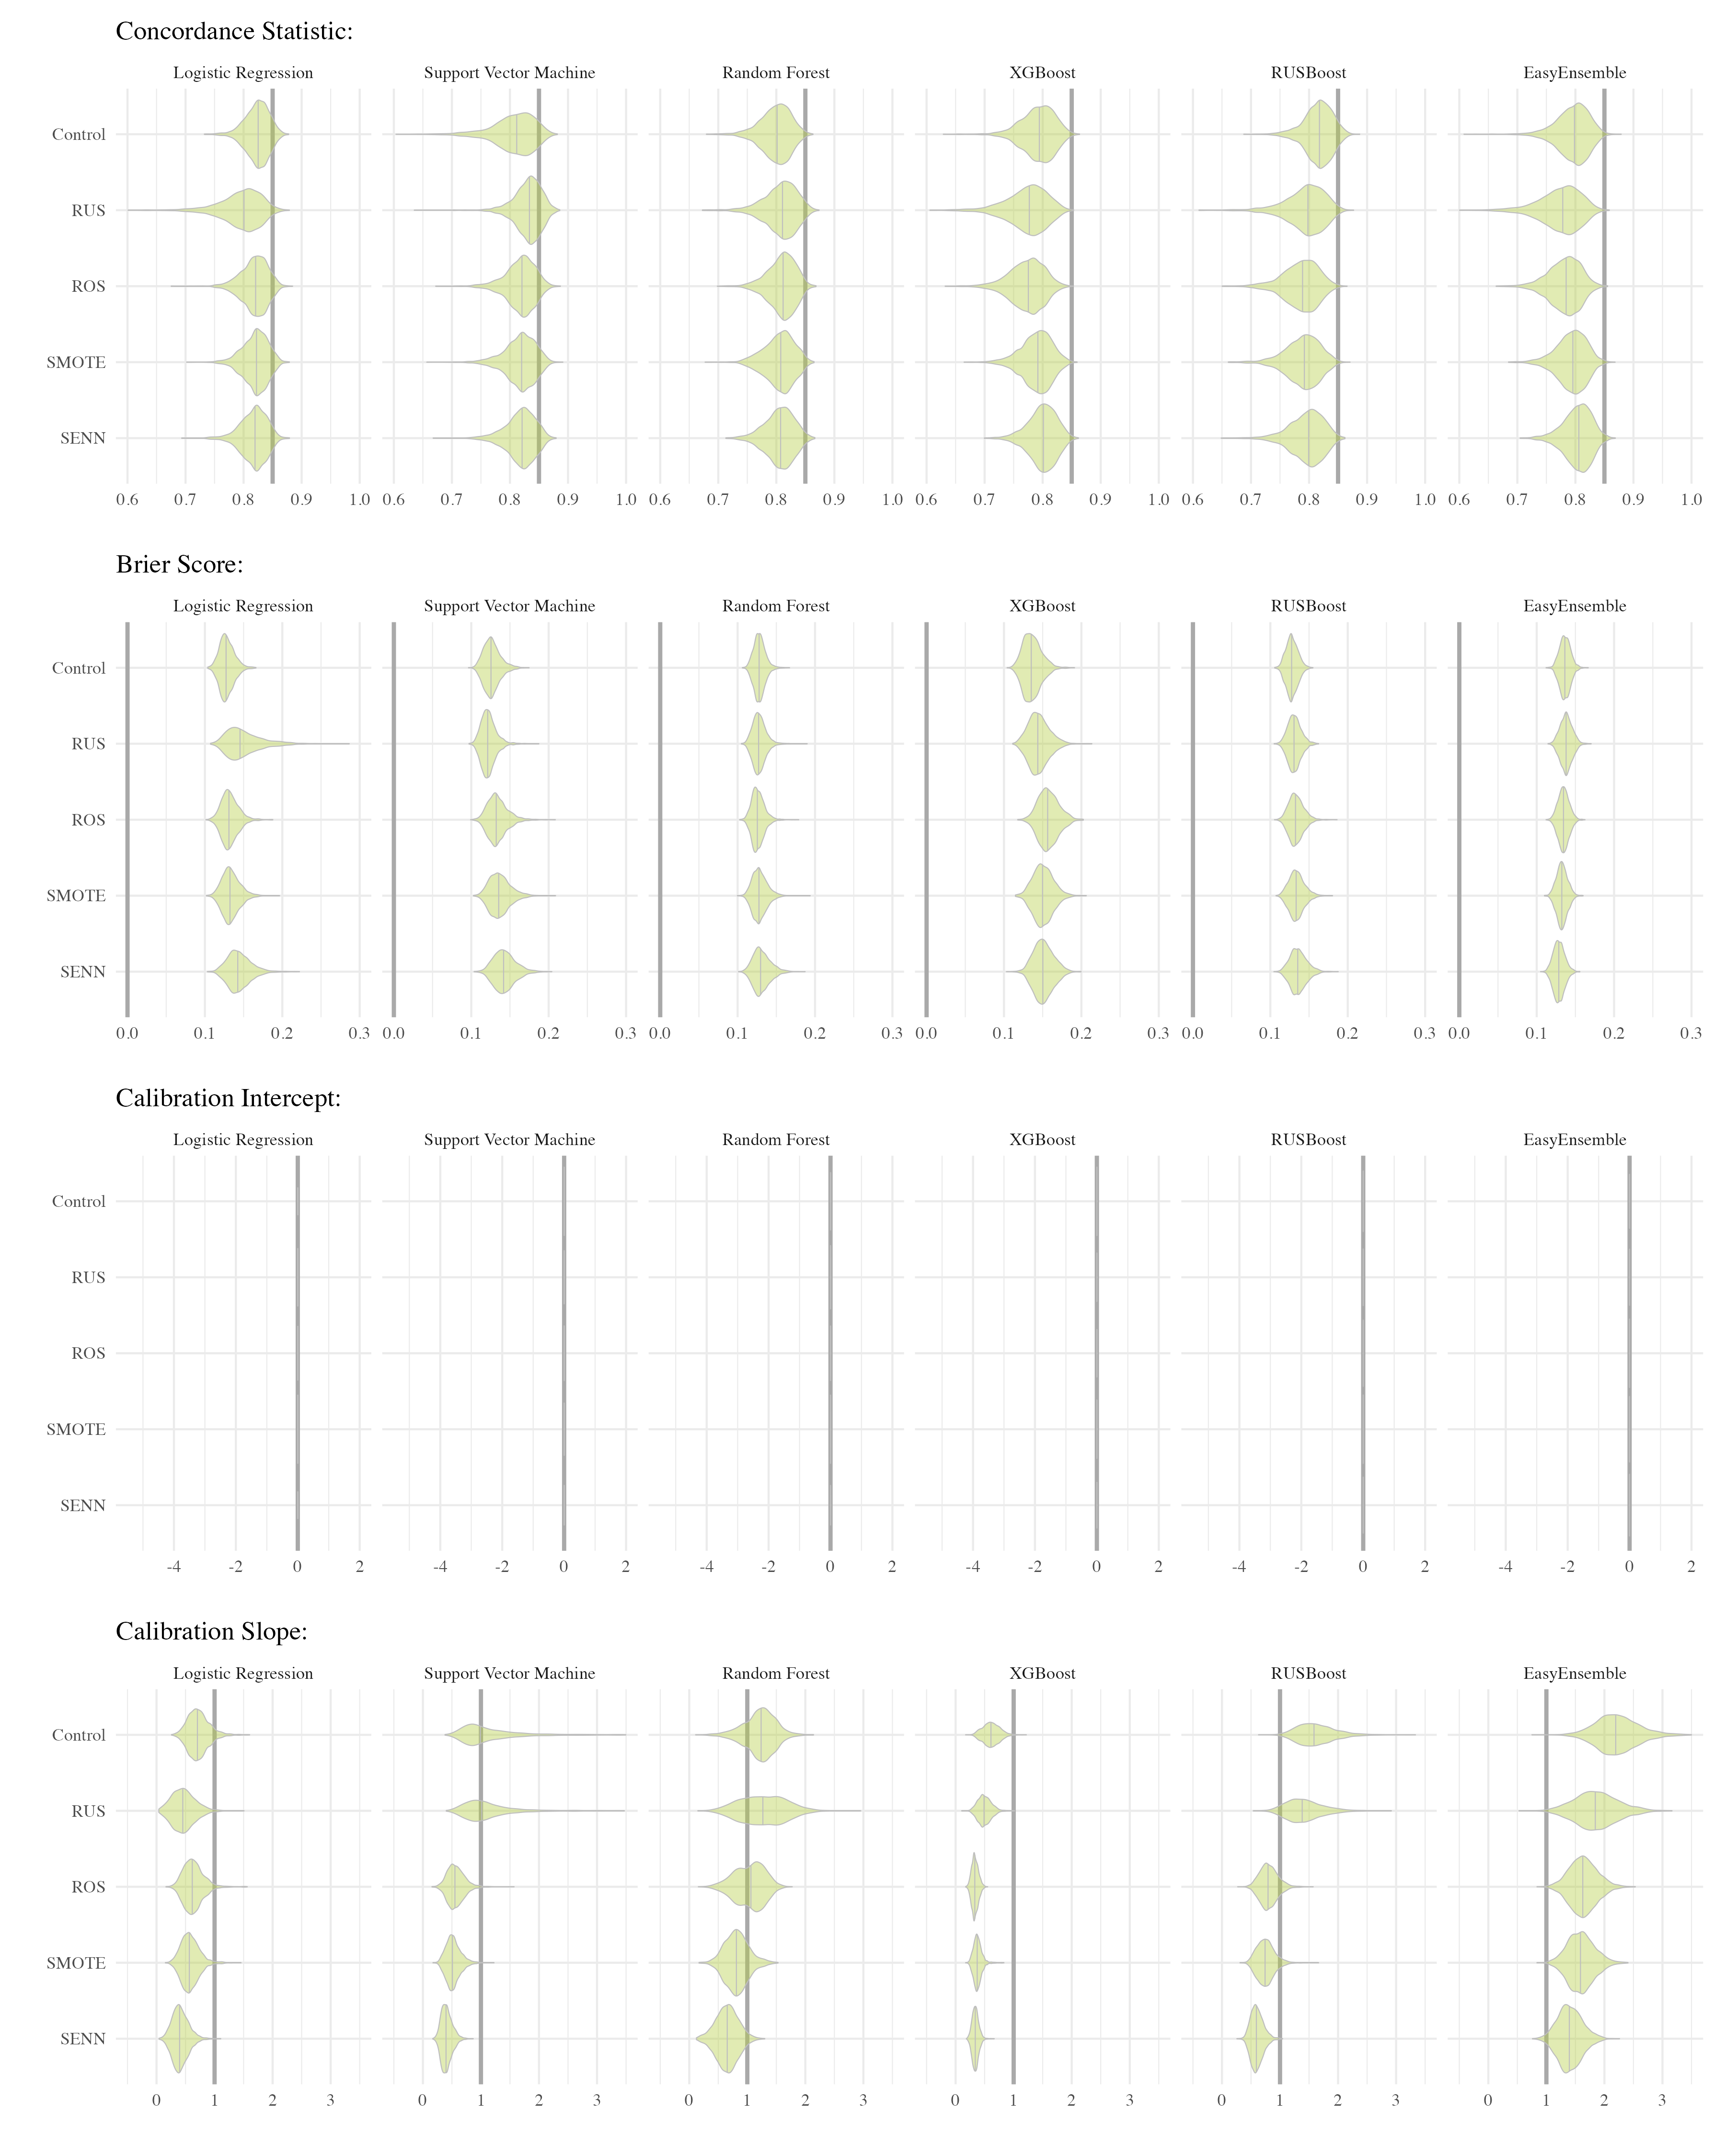
\includegraphics[width=0.7\linewidth]{./figures/performance_metrics_manuscript_sc2_recalibrated} 

}

\caption{Empirical performance metrics for each of 2000 simulation iterations in simulation scenario 2.  This simulation scenario is characterized by 8 predictors, half the required sample size (0.5N) and moderately imbalanced data (event fraction = 0.2). Empirical performance metrics were computed with re-calibrated predicted risks. The target value highlighted for the concordance statistic reflects the data-generating concordance statstic, 0.85. Imbalance corrections: RUS (random undersampling), ROS (random oversampling), SMOTE (synthetic majority oversampling), SENN (synthetic majority oversampling with Wilson's Edited Nearest Neighbors). \label{fig:recal_violin_2}}\label{fig:unnamed-chunk-58}
\end{figure}

\begin{figure}

{\centering 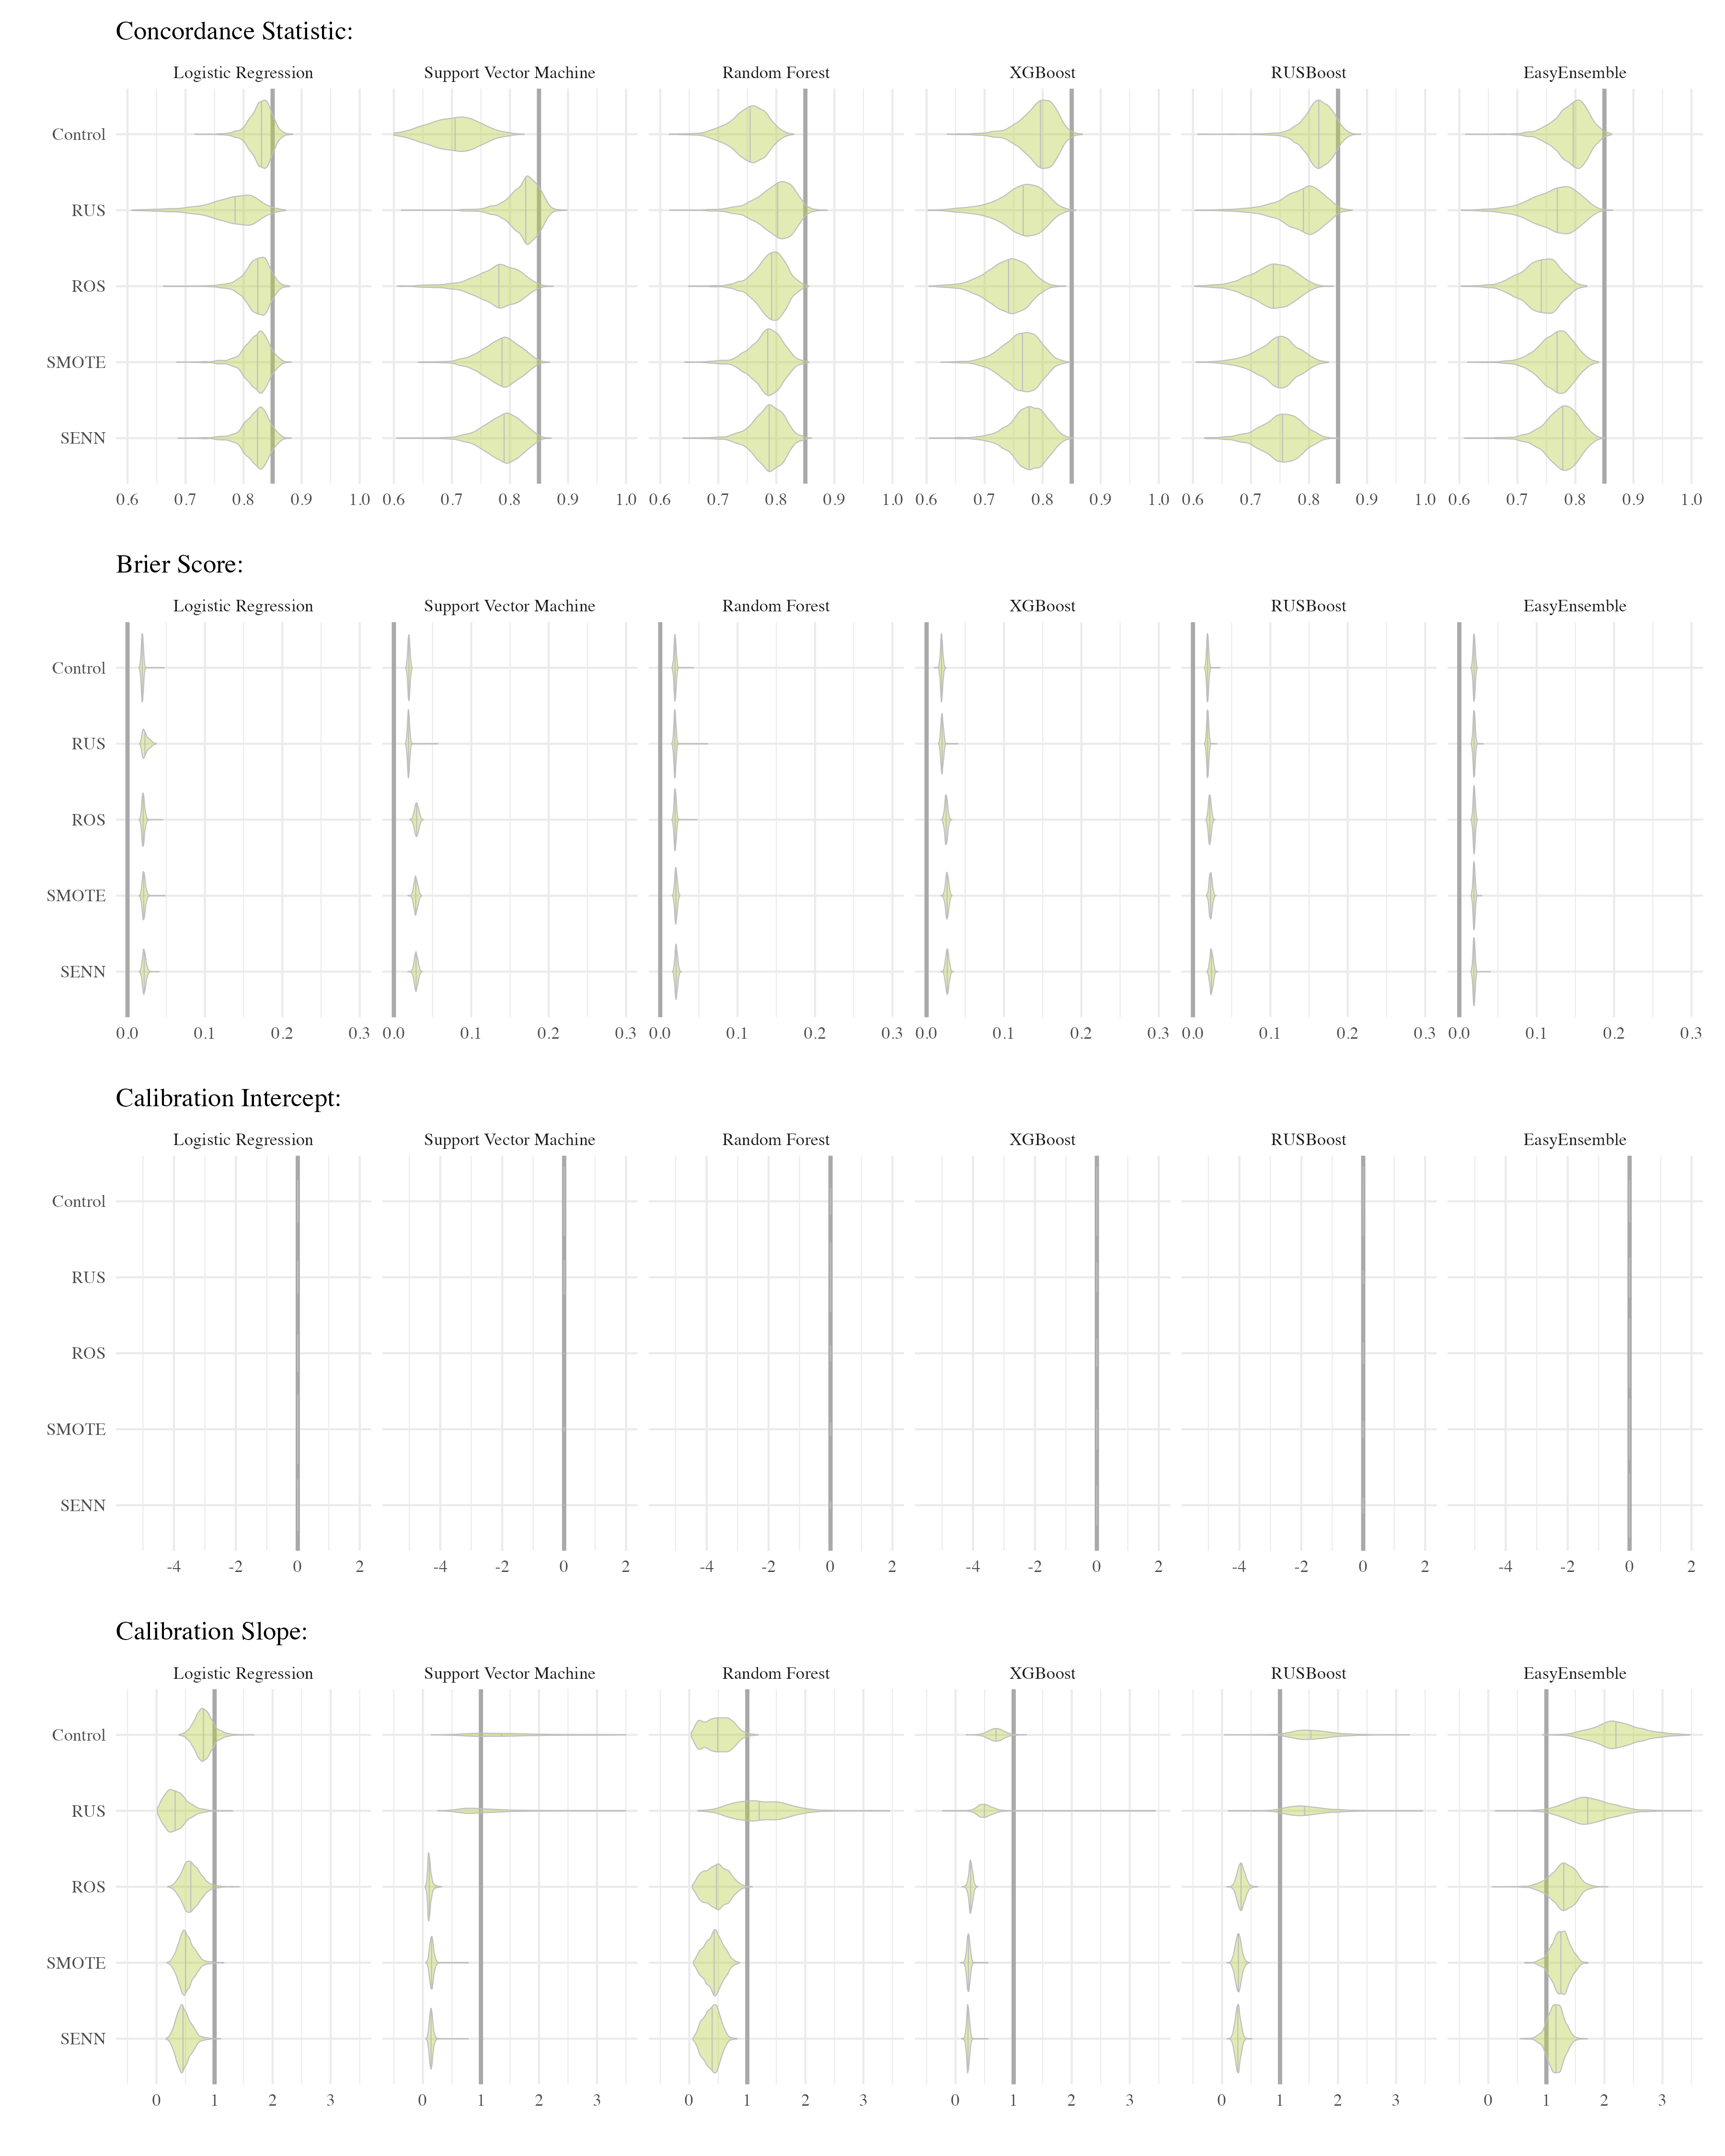
\includegraphics[width=0.7\linewidth]{./figures/performance_metrics_manuscript_sc3_recalibrated} 

}

\caption{Empirical performance metrics for each of 2000 simulation iterations in simulation scenario 3.  This simulation scenario is characterized by 8 predictors, half the required sample size (0.5N) and strongly imbalanced data (event fraction = 0.02). Empirical performance metrics were computed with re-calibrated predicted risks. The target value highlighted for the concordance statistic reflects the data-generating concordance statstic, 0.85. Imbalance corrections: RUS (random undersampling), ROS (random oversampling), SMOTE (synthetic majority oversampling), SENN (synthetic majority oversampling with Wilson's Edited Nearest Neighbors). Note: after re-calibration, calibration intercepts were essentially zero for every iteration and are therefore not visible on the plot.  \label{fig:recal_violin_3}}\label{fig:unnamed-chunk-59}
\end{figure}

\begin{figure}

{\centering 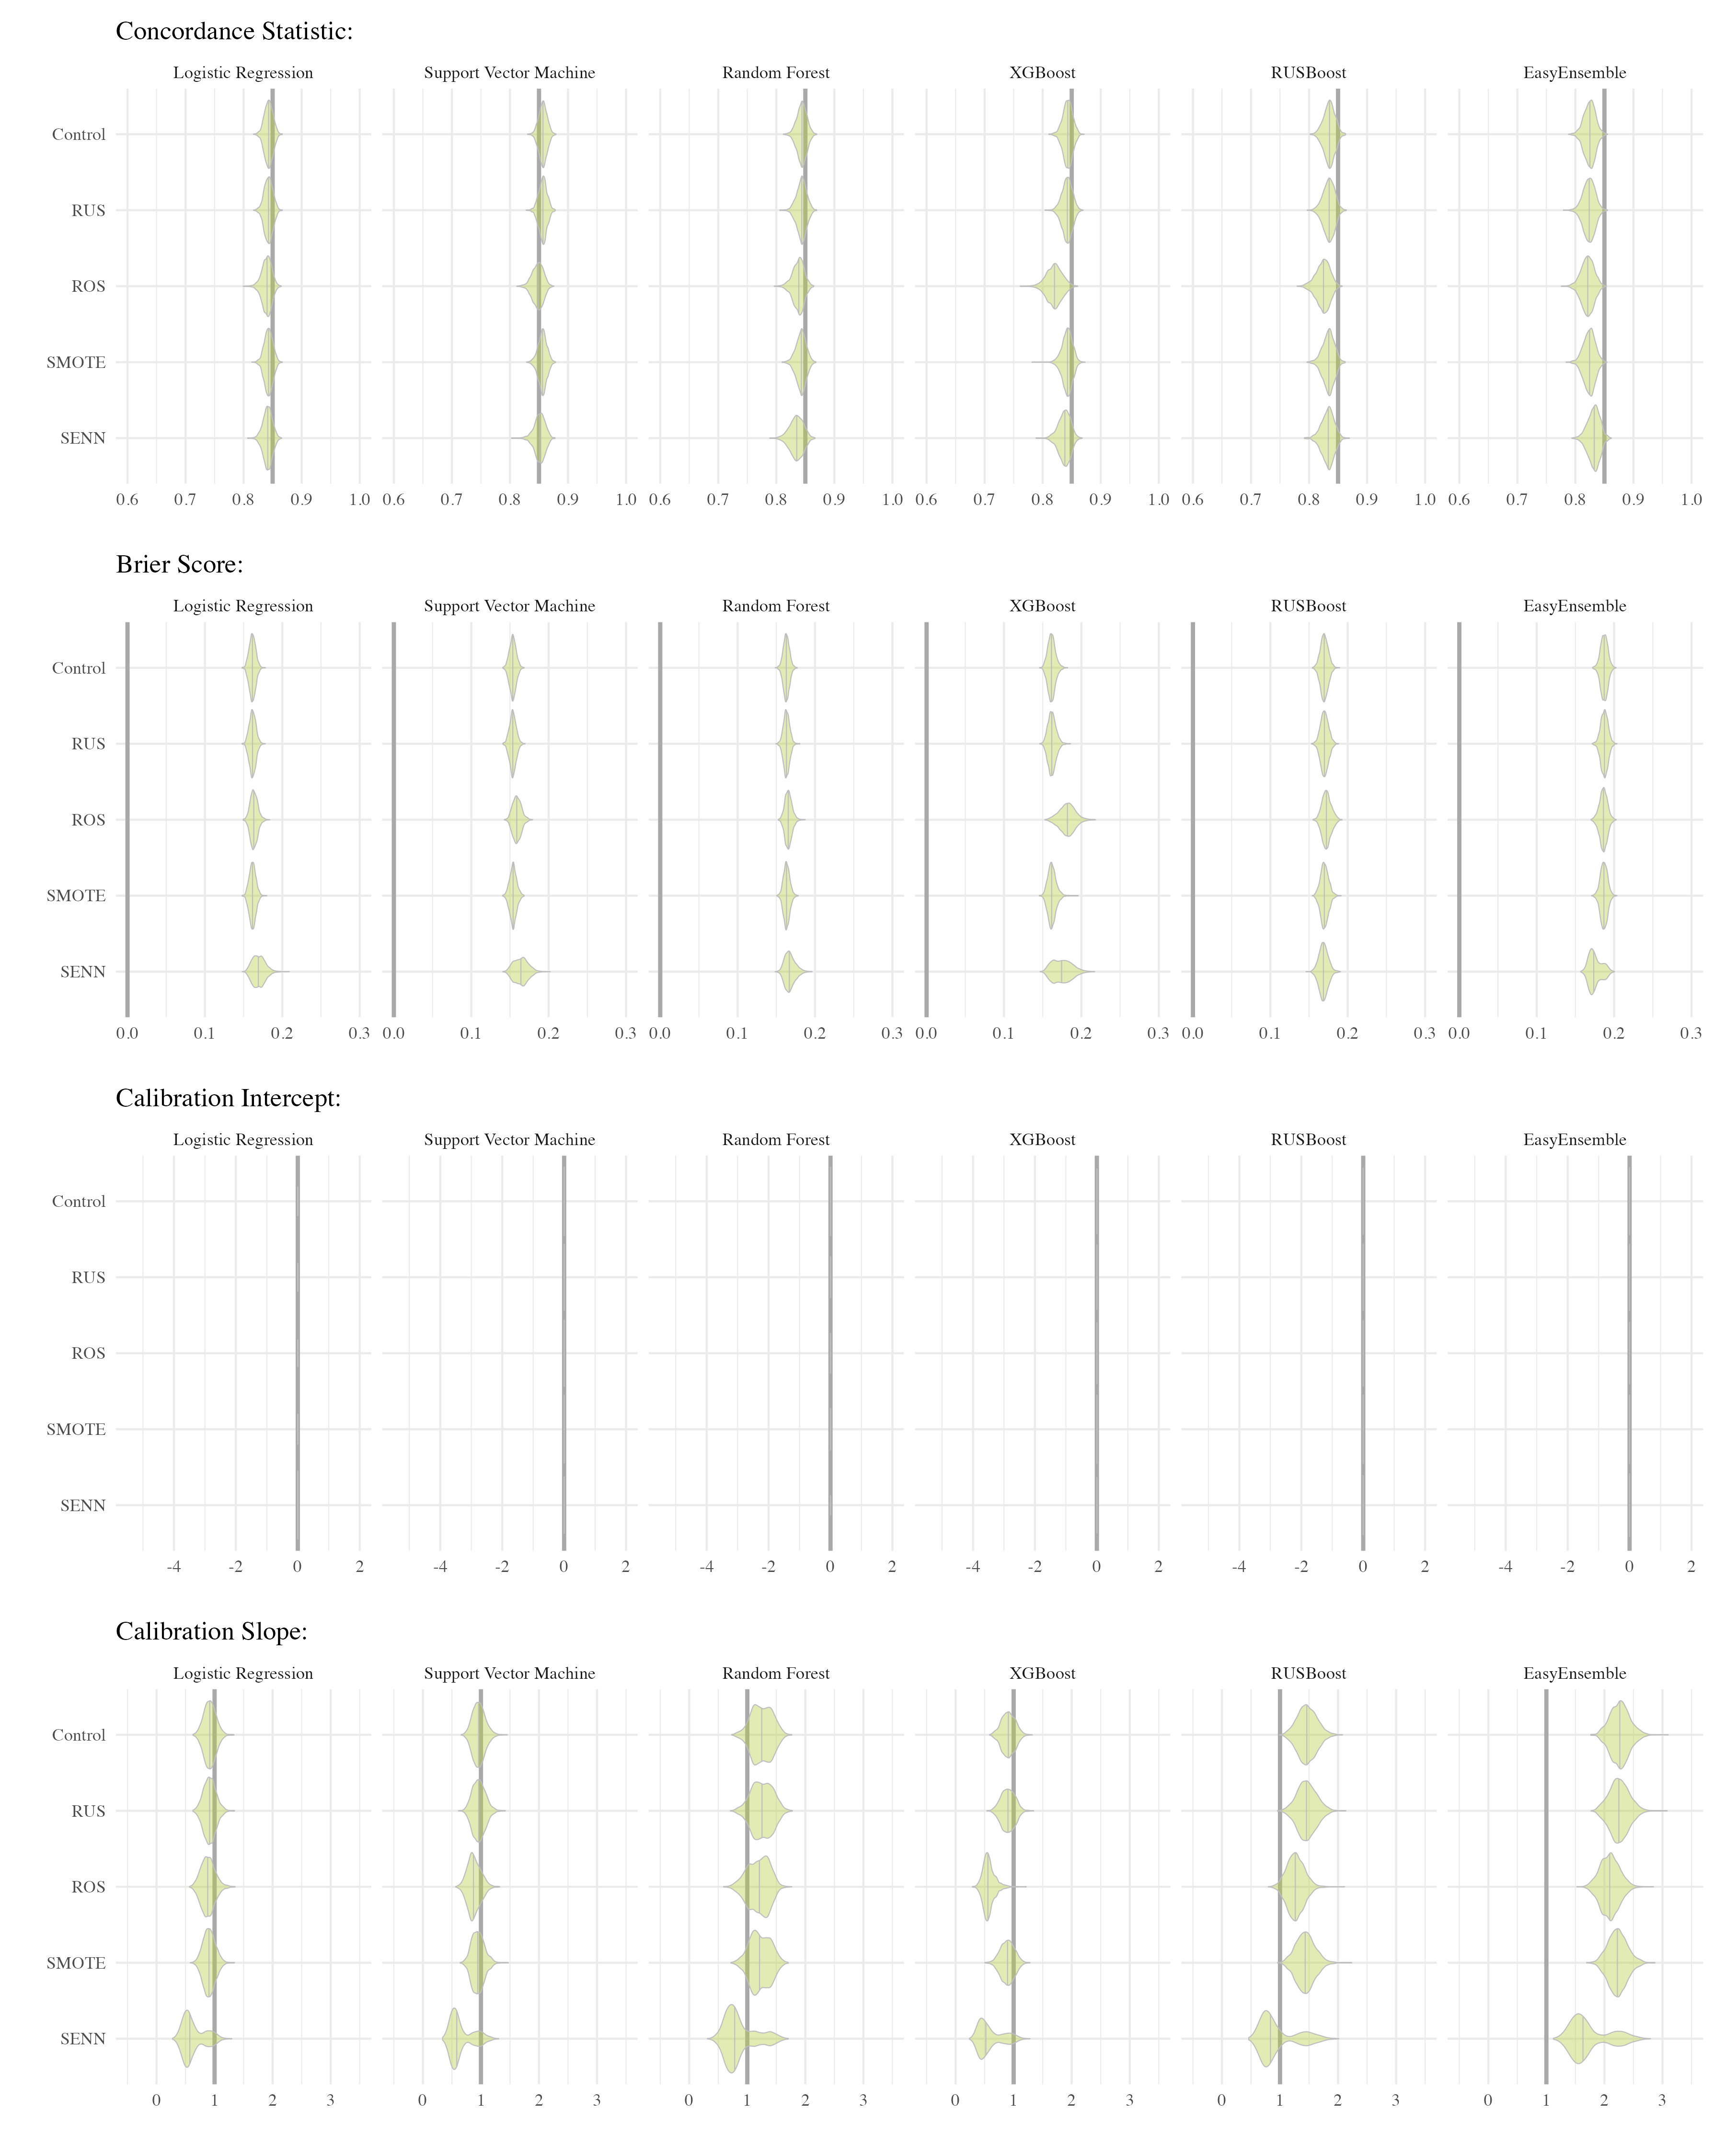
\includegraphics[width=0.7\linewidth]{./figures/performance_metrics_manuscript_sc4_recalibrated} 

}

\caption{Empirical performance metrics for each of 2000 simulation iterations in simulation scenario 4.  This simulation scenario is characterized by 8 predictors, minimum required sample size (N) and class balanced data (event fraction = 0.5). Empirical performance metrics were computed with re-calibrated predicted risks. The target value highlighted for the concordance statistic reflects the data-generating concordance statstic, 0.85. Imbalance corrections: RUS (random undersampling), ROS (random oversampling), SMOTE (synthetic majority oversampling), SENN (synthetic majority oversampling with Wilson's Edited Nearest Neighbors). Note: after re-calibration, calibration intercepts were essentially zero for every iteration and are therefore not visible on the plot.  \label{fig:recal_violin_4}}\label{fig:unnamed-chunk-60}
\end{figure}

\begin{figure}

{\centering 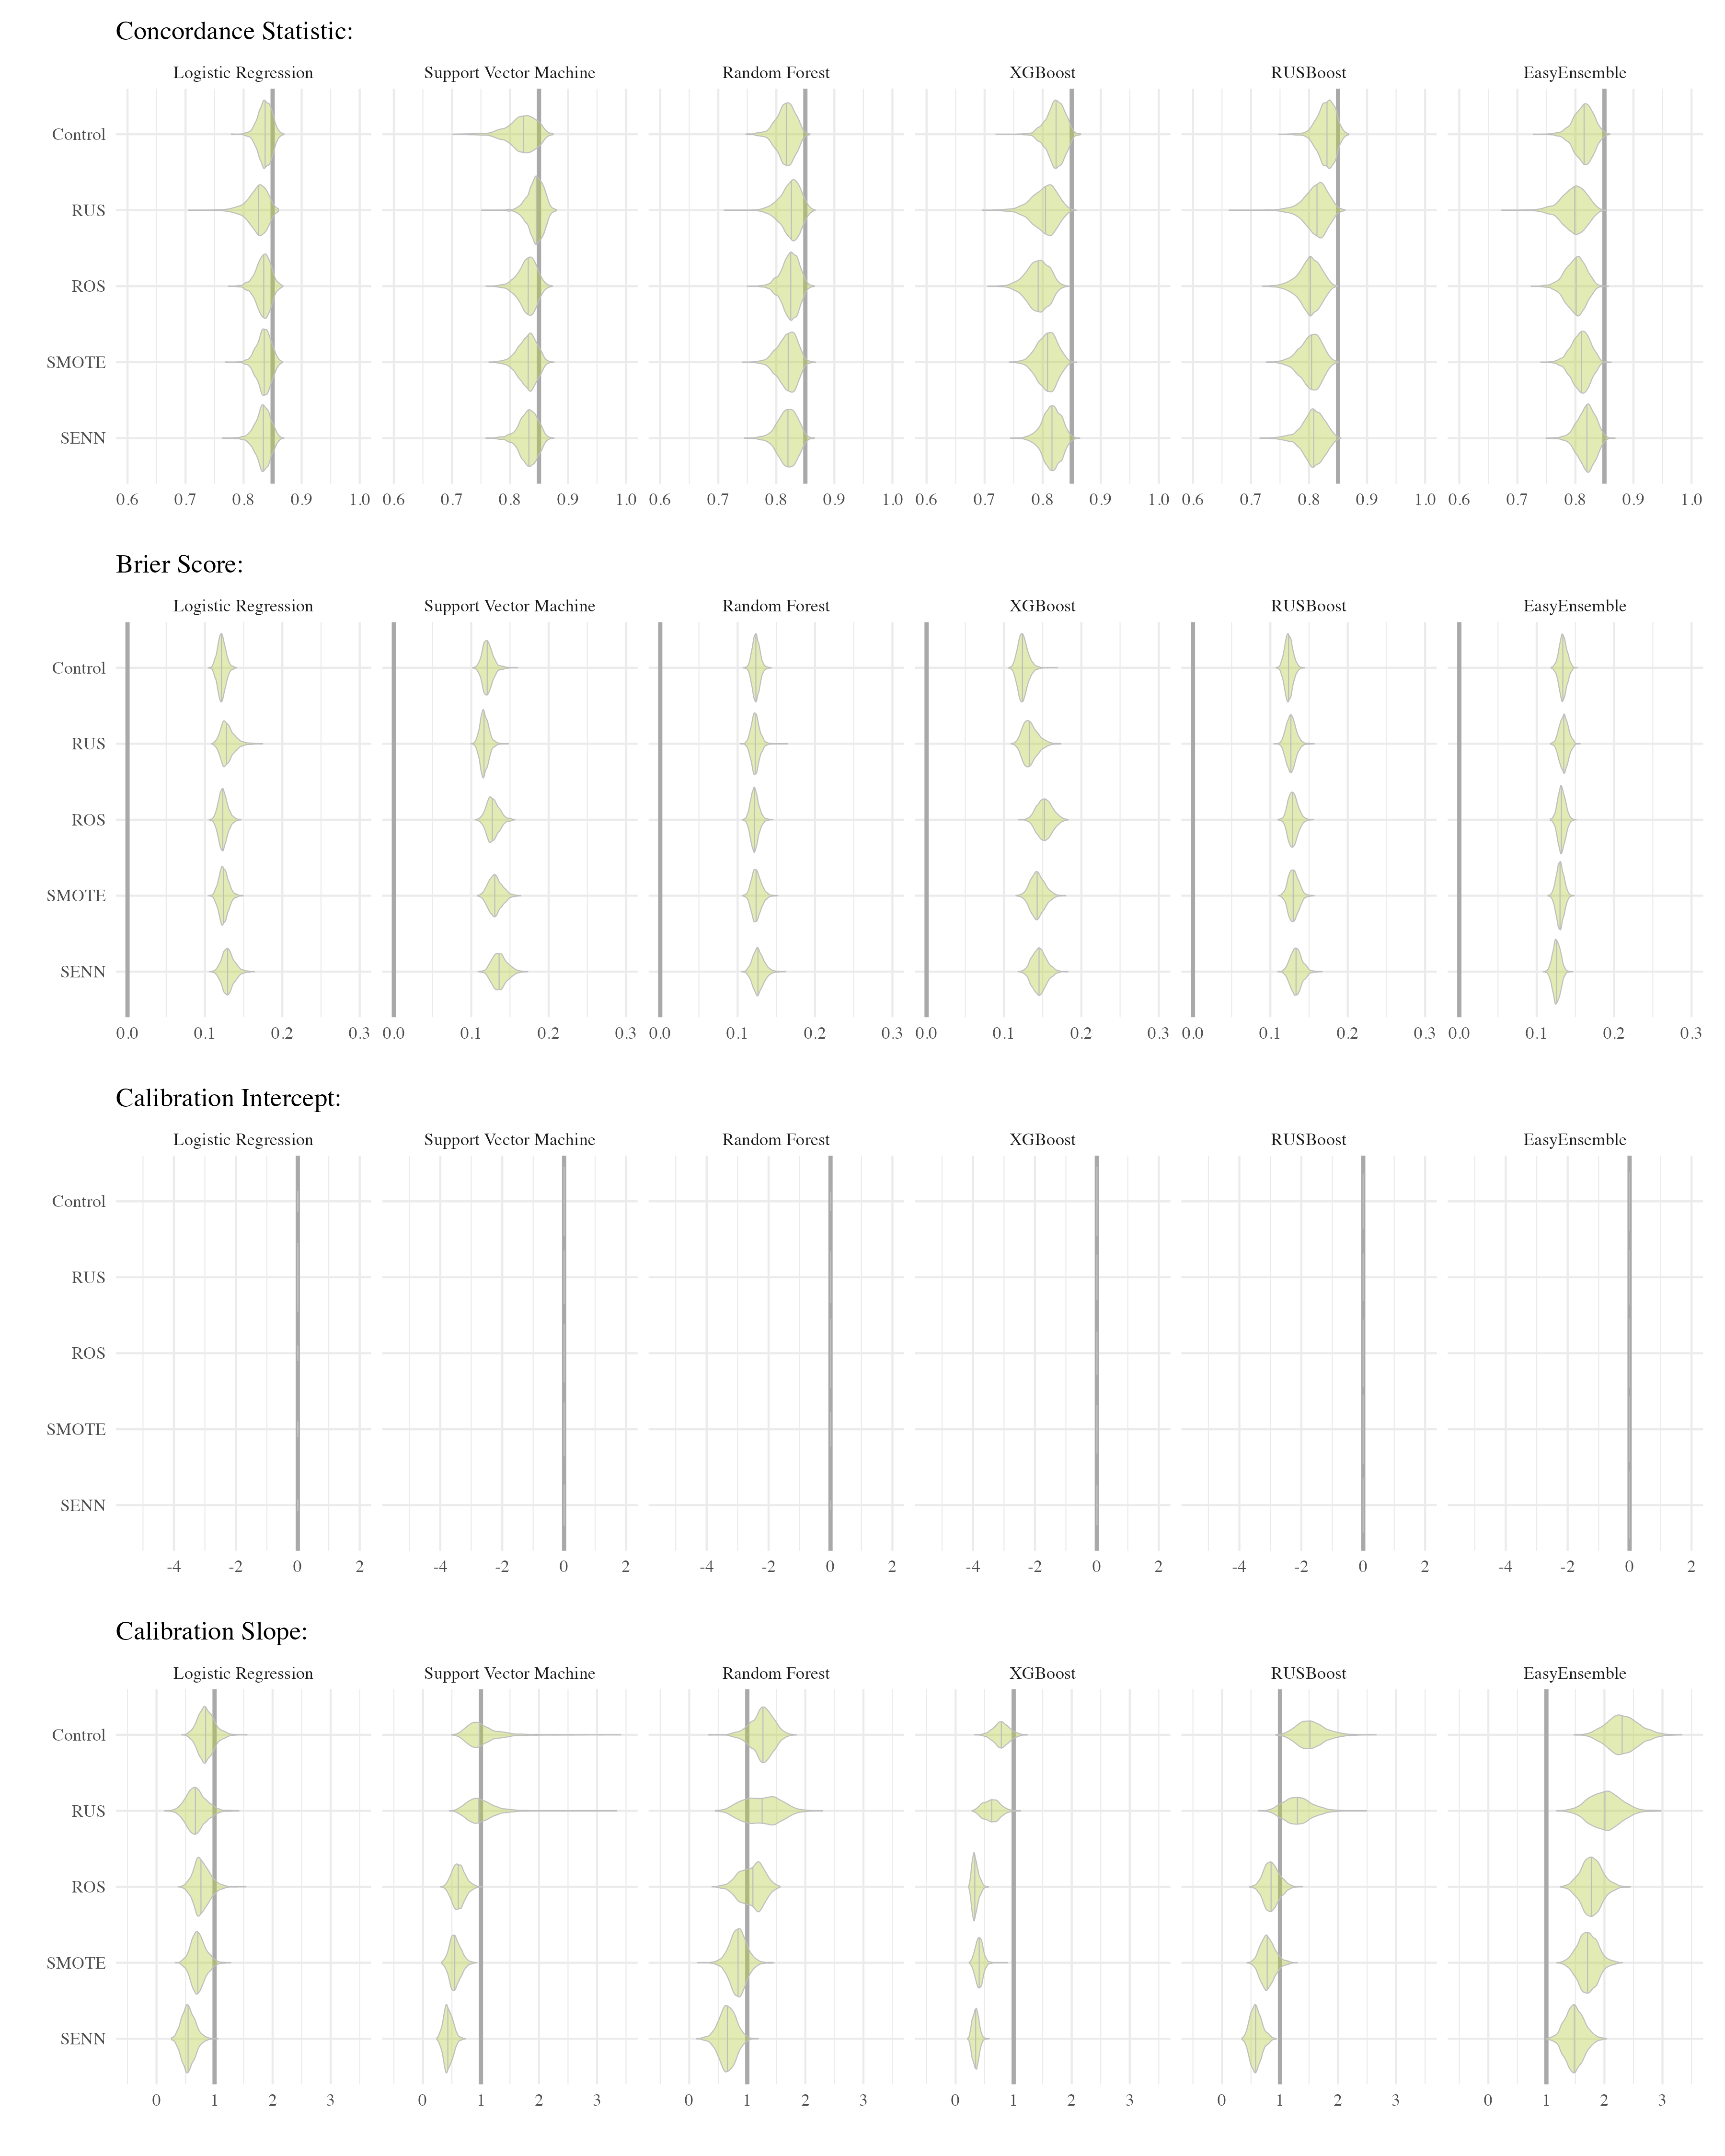
\includegraphics[width=0.7\linewidth]{./figures/performance_metrics_manuscript_sc5_recalibrated} 

}

\caption{Empirical performance metrics for each of 2000 simulation iterations in simulation scenario 5.  This simulation scenario is characterized by 8 predictors, minimum required sample size (N) and moderately imbalanced data (event fraction = 0.2). Empirical performance metrics were computed with re-calibrated predicted risks. The target value highlighted for the concordance statistic reflects the data-generating concordance statstic, 0.85. Imbalance corrections: RUS (random undersampling), ROS (random oversampling), SMOTE (synthetic majority oversampling), SENN (synthetic majority oversampling with Wilson's Edited Nearest Neighbors). Note: after re-calibration, calibration intercepts were essentially zero for every iteration and are therefore not visible on the plot.  \label{fig:recal_violin_5}}\label{fig:unnamed-chunk-61}
\end{figure}

\begin{figure}

{\centering 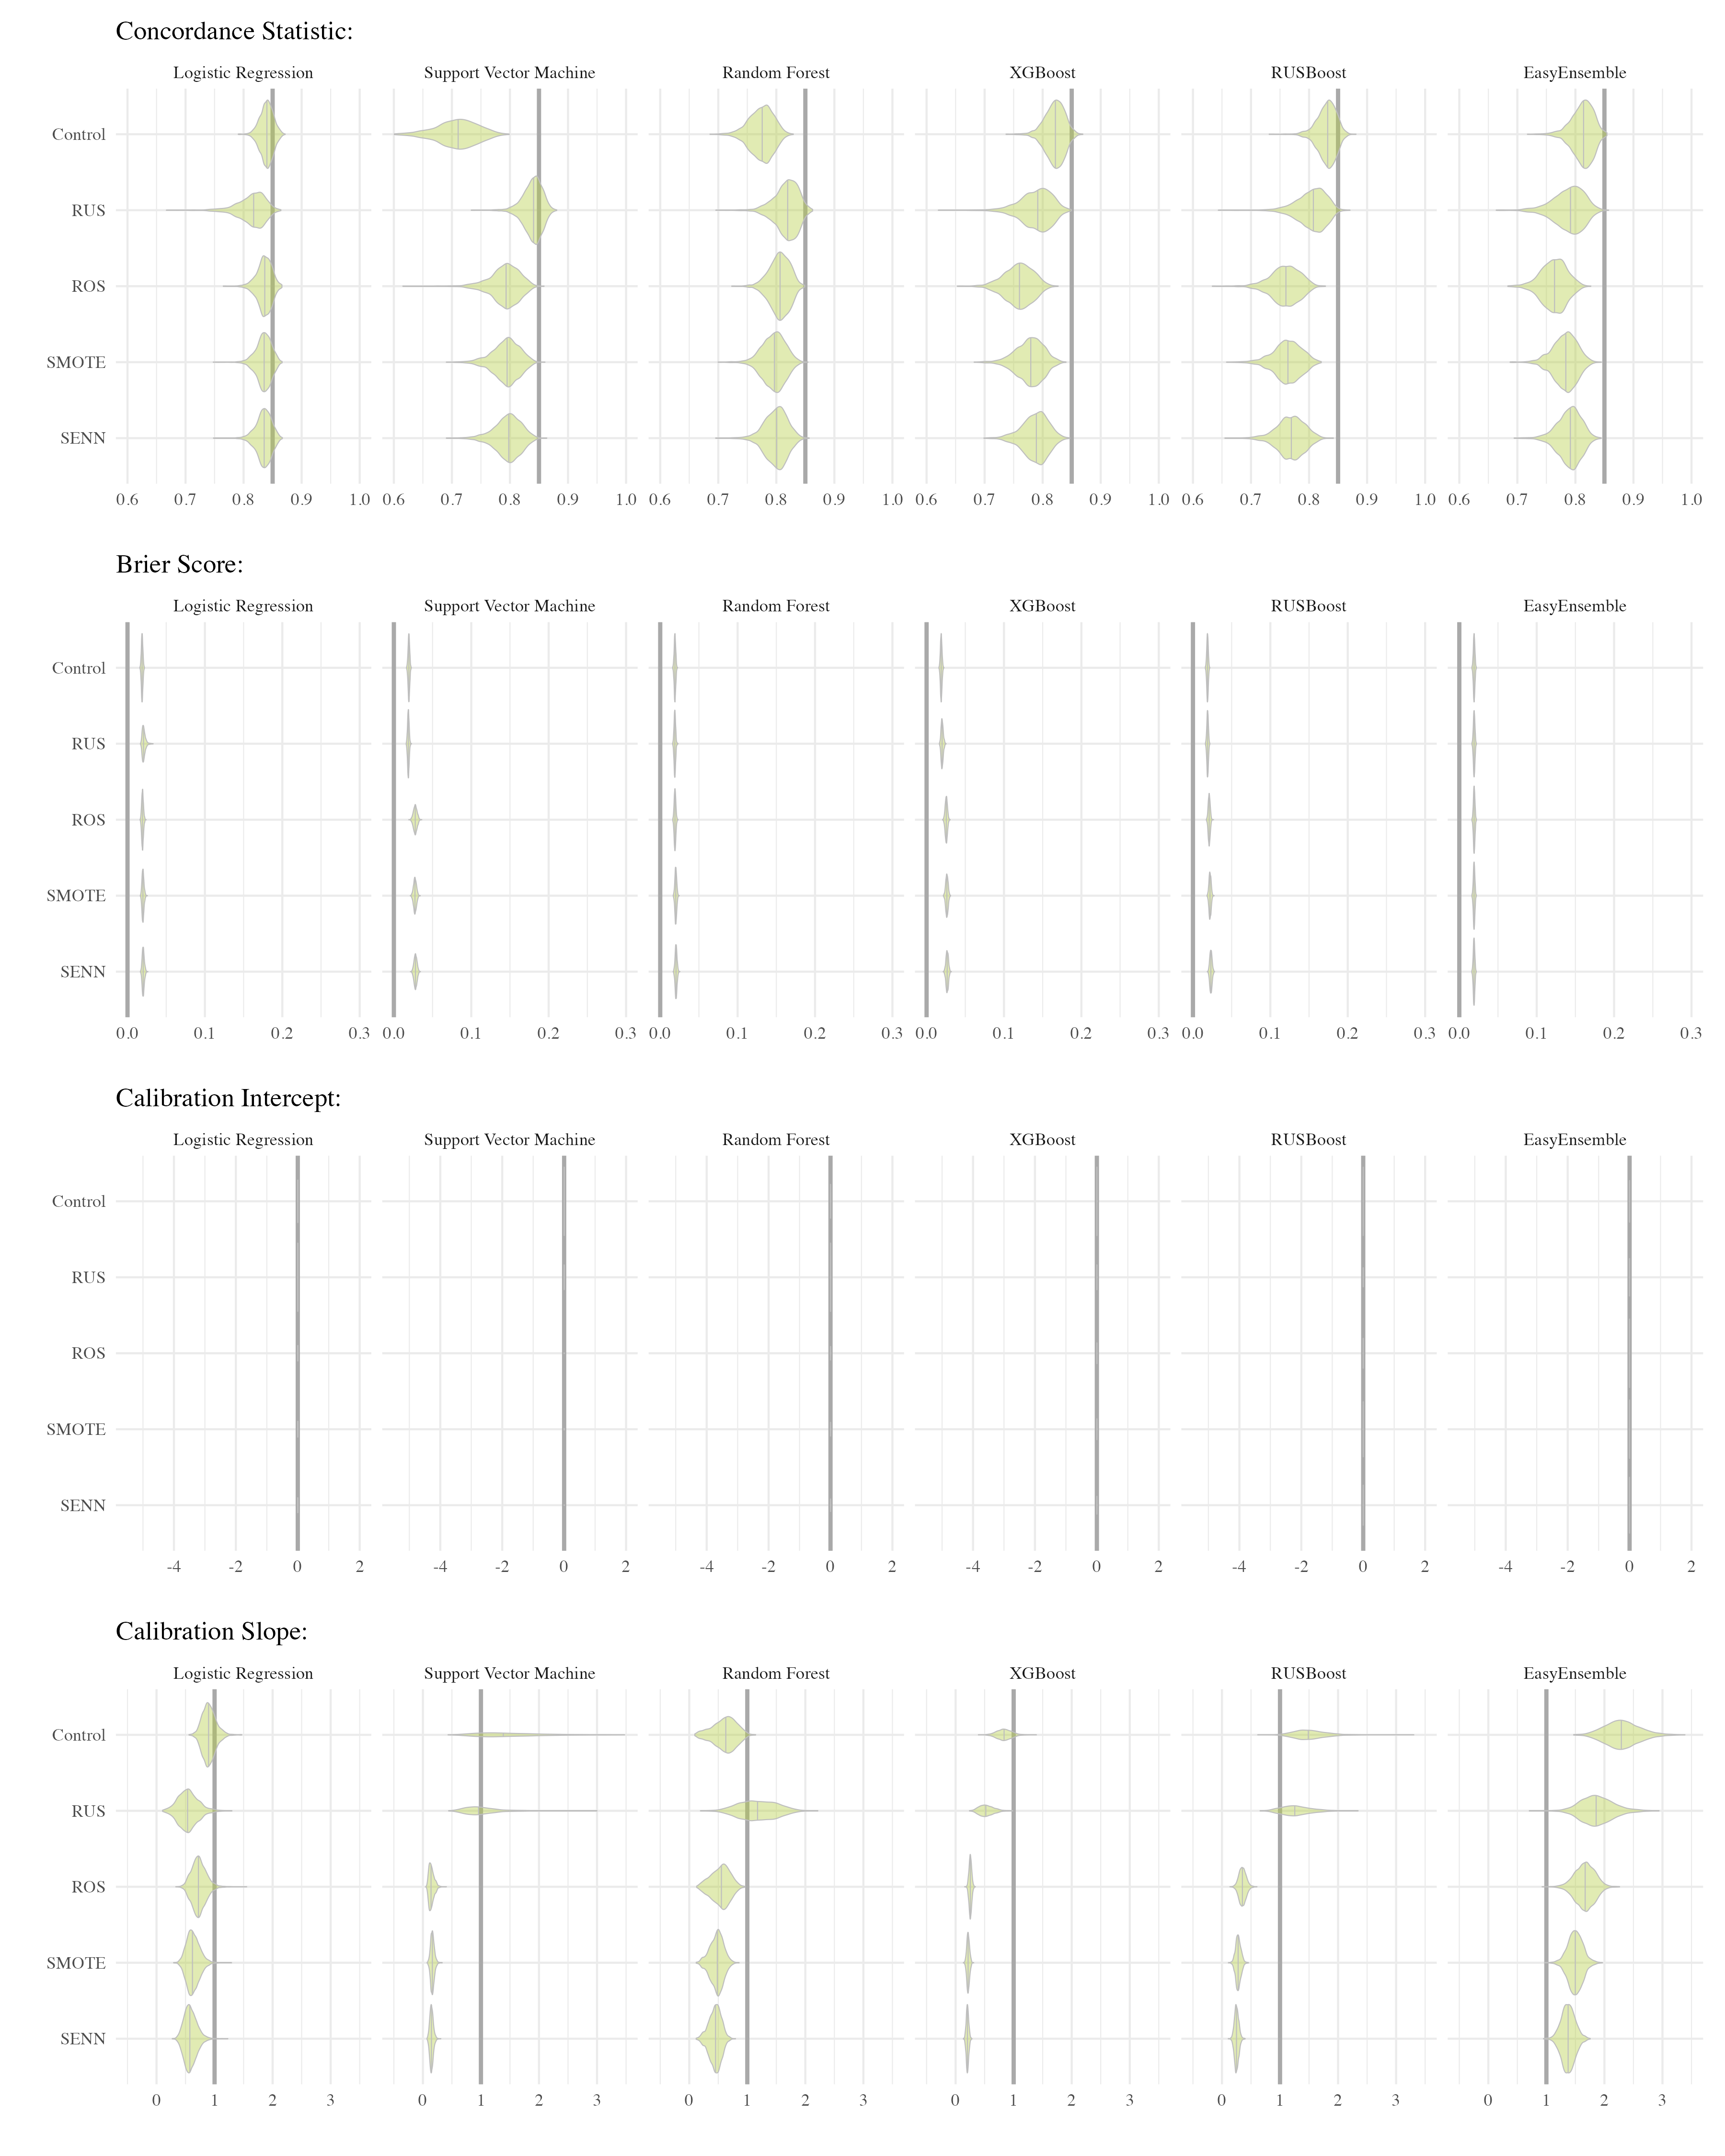
\includegraphics[width=0.7\linewidth]{./figures/performance_metrics_manuscript_sc6_recalibrated} 

}

\caption{Empirical performance metrics for each of 2000 simulation iterations in simulation scenario 6.  This simulation scenario is characterized by 8 predictors, minimum required sample size (N) and strongly imbalanced data (event fraction = 0.02). Empirical performance metrics were computed with re-calibrated predicted risks. The target value highlighted for the concordance statistic reflects the data-generating concordance statstic, 0.85. Imbalance corrections: RUS (random undersampling), ROS (random oversampling), SMOTE (synthetic majority oversampling), SENN (synthetic majority oversampling with Wilson's Edited Nearest Neighbors). Note: after re-calibration, calibration intercepts were essentially zero for every iteration and are therefore not visible on the plot.  \label{fig:recal_violin_6}}\label{fig:unnamed-chunk-62}
\end{figure}

\begin{figure}

{\centering 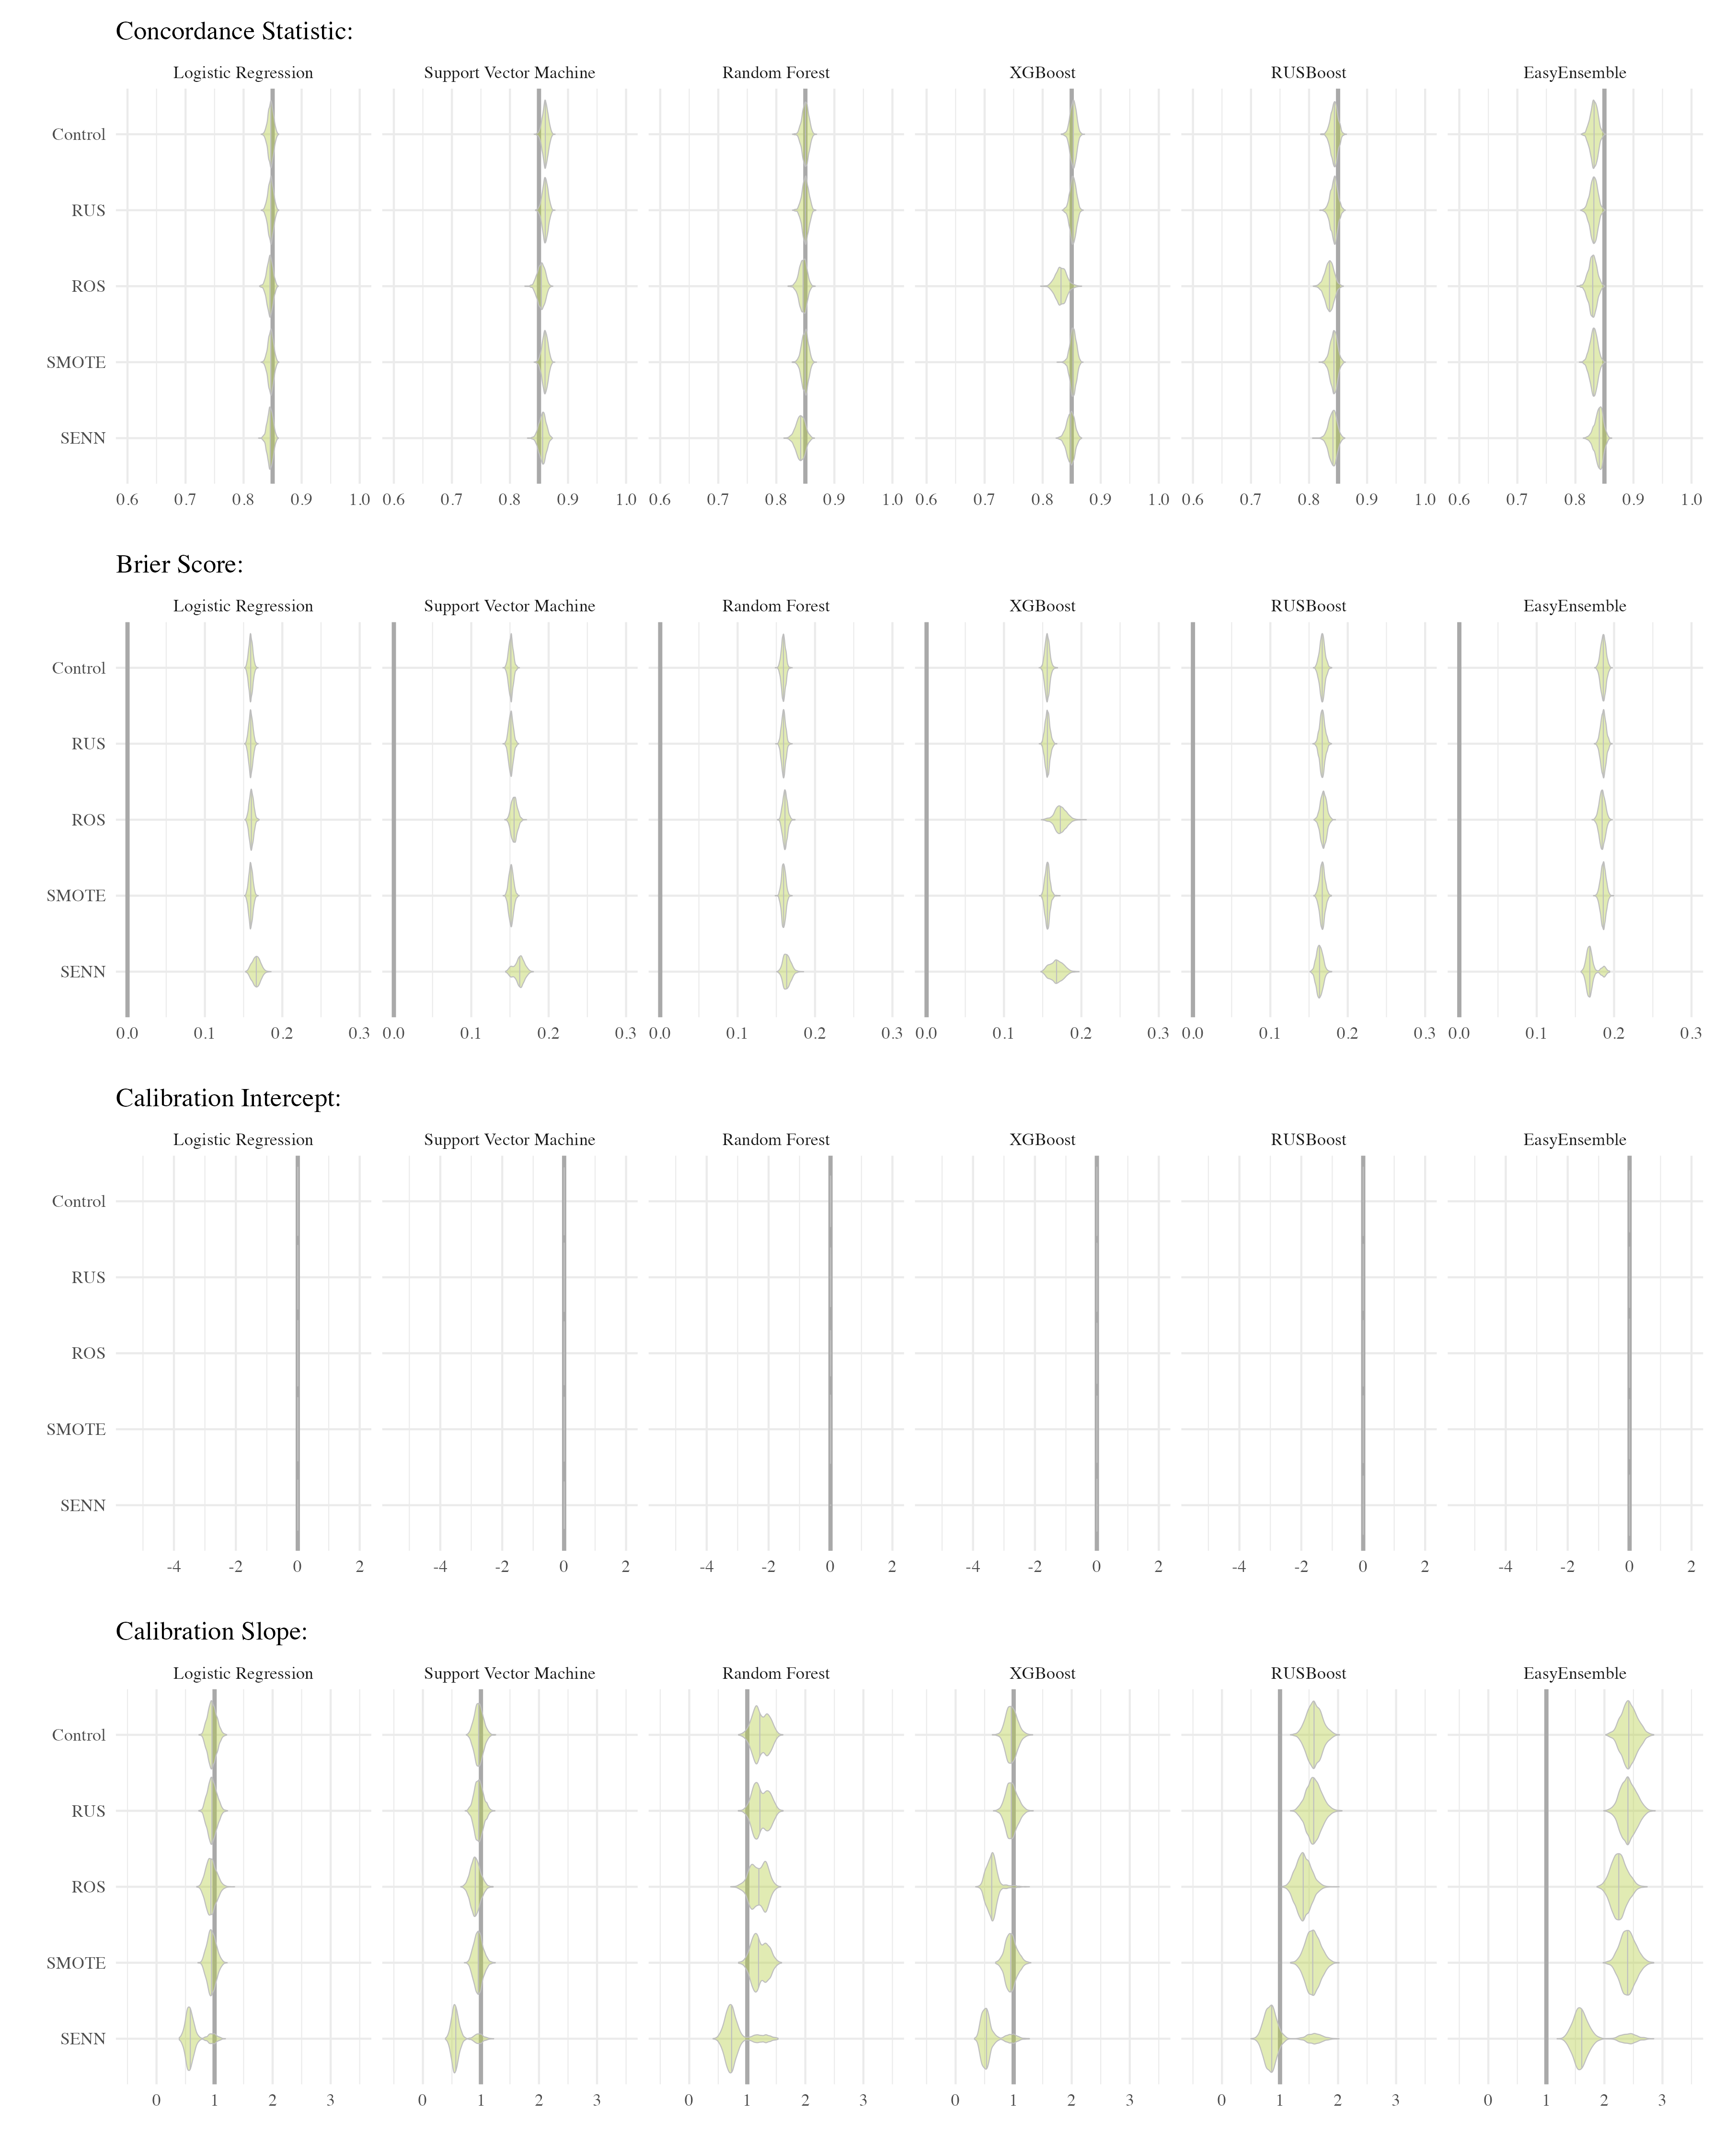
\includegraphics[width=0.7\linewidth]{./figures/performance_metrics_manuscript_sc7_recalibrated} 

}

\caption{Empirical performance metrics for each of 2000 simulation iterations in simulation scenario 7.  This simulation scenario is characterized by 8 predictors, double the required sample size (2N) and class balanced data (event fraction = 0.5). Empirical performance metrics were computed with re-calibrated predicted risks. The target value highlighted for the concordance statistic reflects the data-generating concordance statstic, 0.85. Imbalance corrections: RUS (random undersampling), ROS (random oversampling), SMOTE (synthetic majority oversampling), SENN (synthetic majority oversampling with Wilson's Edited Nearest Neighbors). Note: after re-calibration, calibration intercepts were essentially zero for every iteration and are therefore not visible on the plot.  \label{fig:recal_violin_7}}\label{fig:unnamed-chunk-63}
\end{figure}

\begin{figure}

{\centering 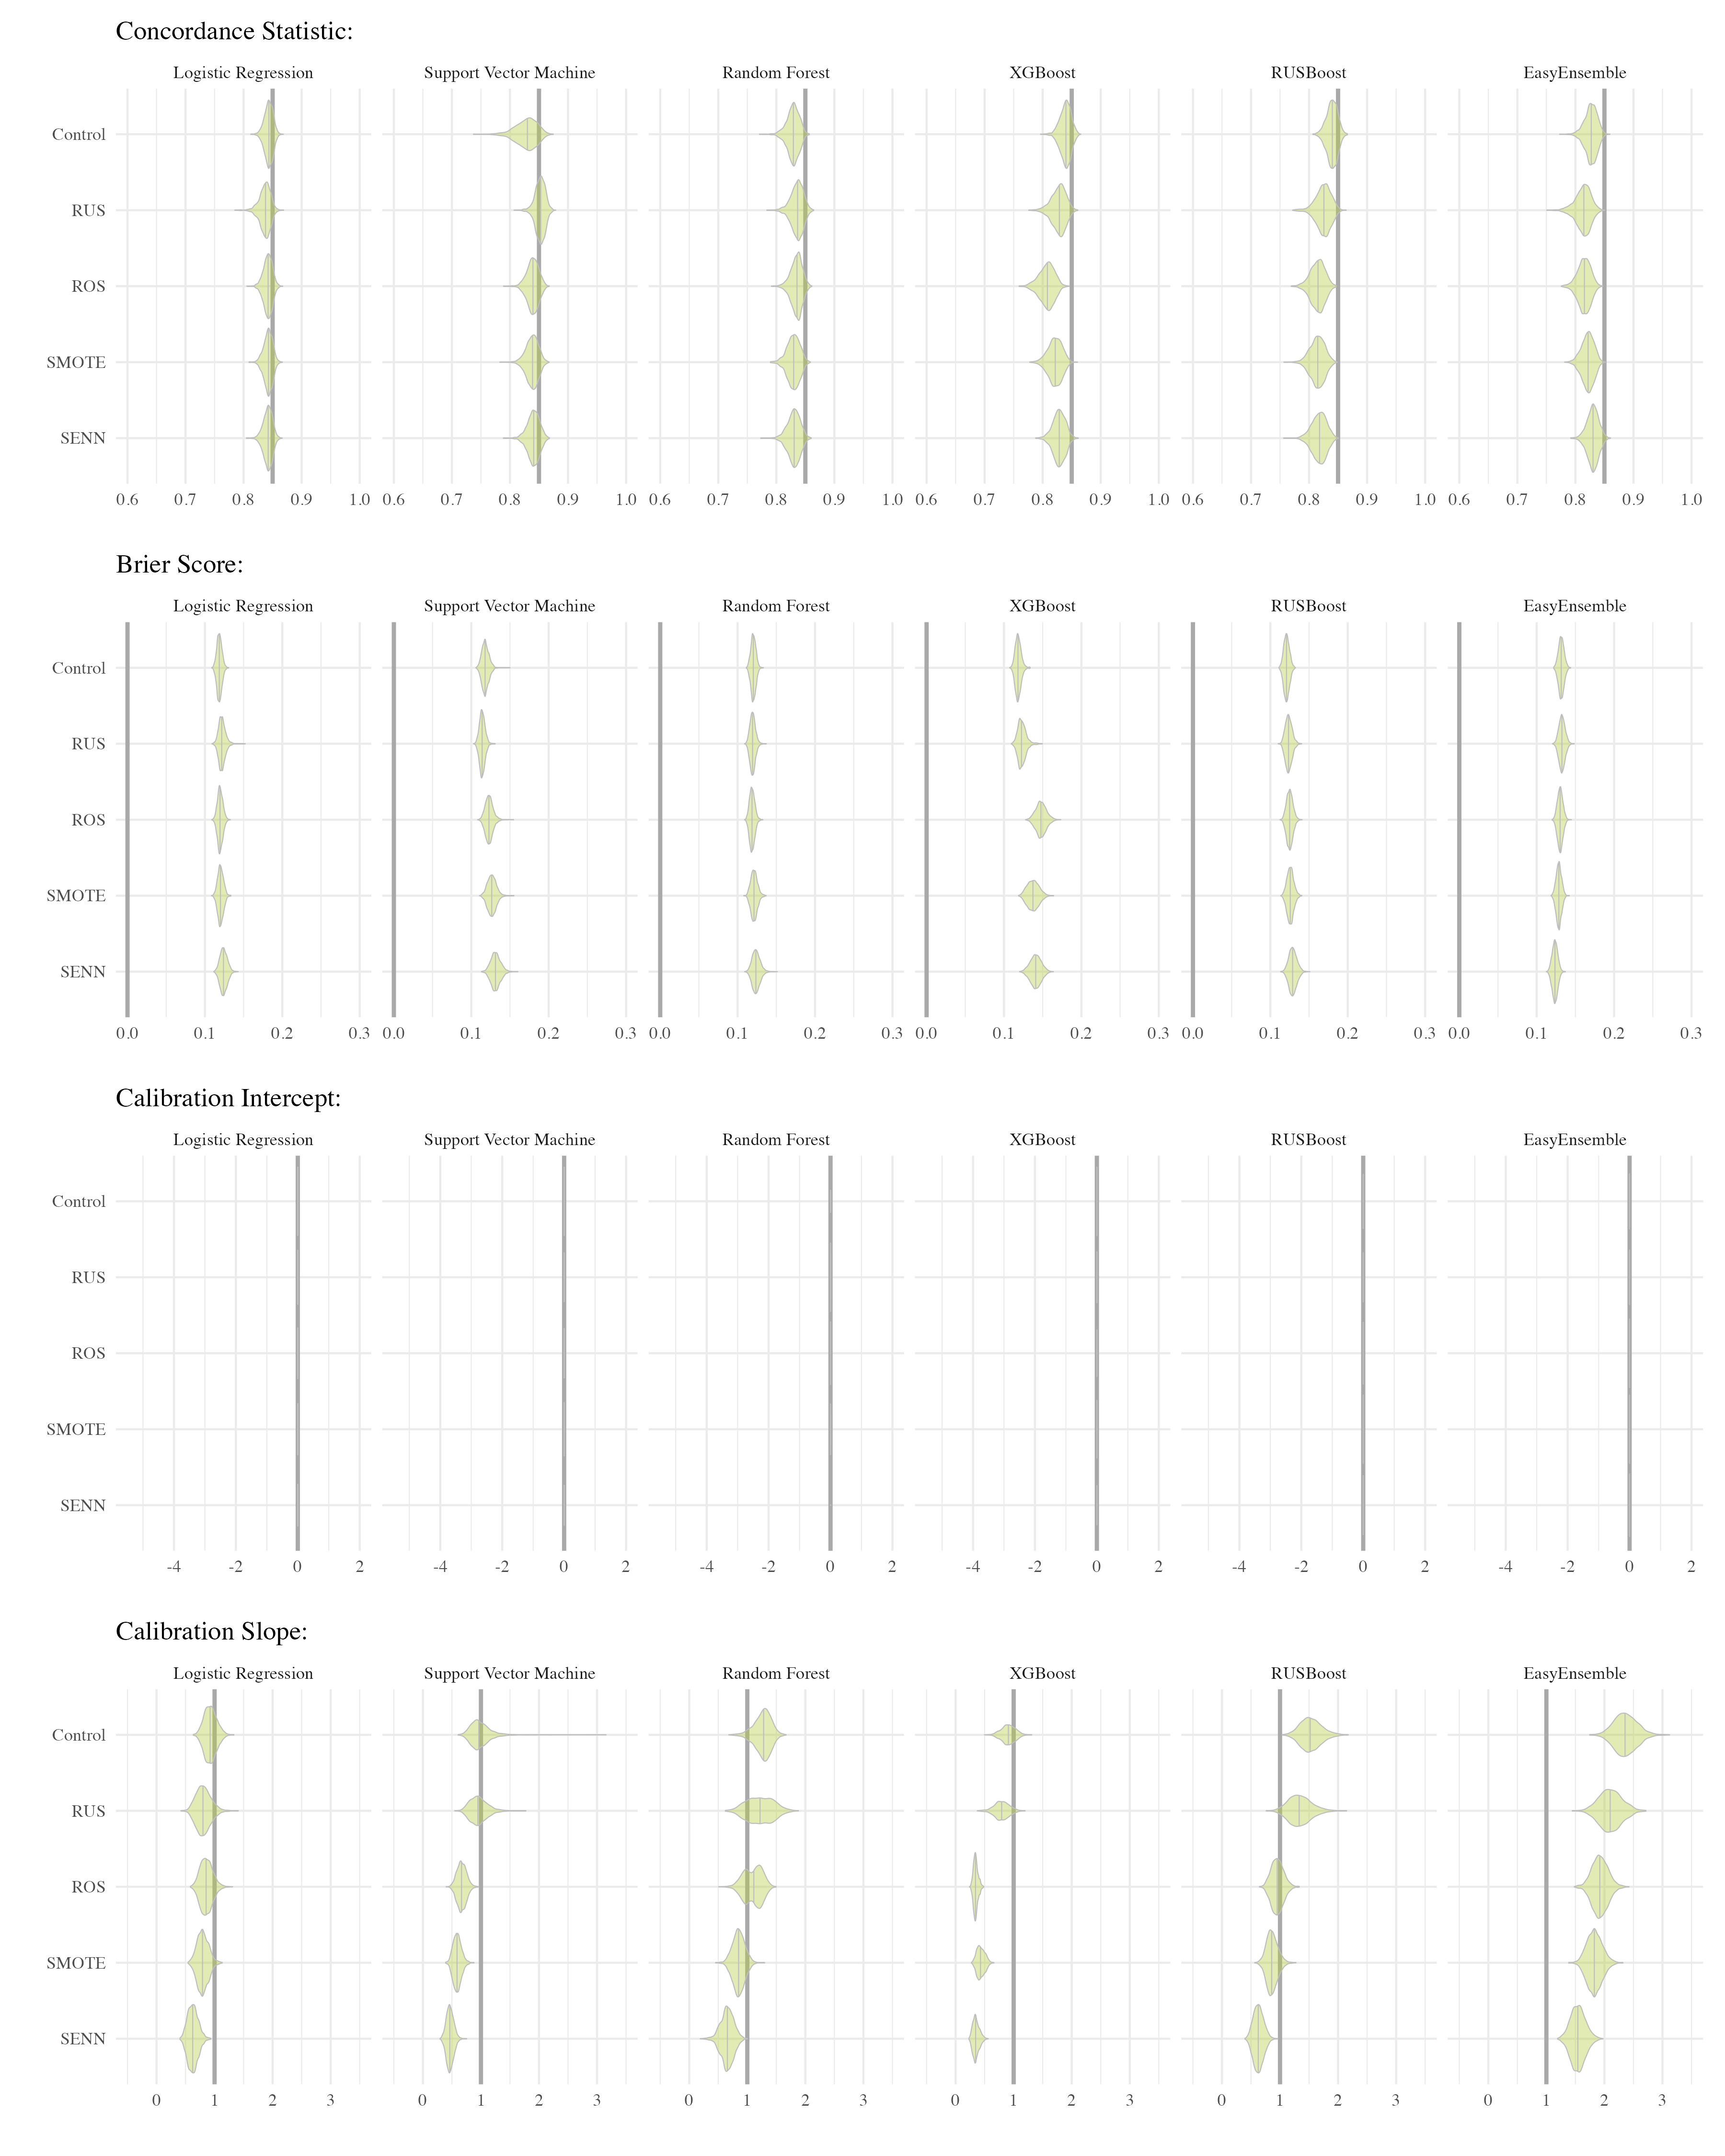
\includegraphics[width=0.7\linewidth]{./figures/performance_metrics_manuscript_sc8_recalibrated} 

}

\caption{Empirical performance metrics for each of 2000 simulation iterations in simulation scenario 8.  This simulation scenario is characterized by 8 predictors, double the required sample size (2N) and moderately imbalanced data (event fraction = 0.2). Empirical performance metrics were computed with re-calibrated predicted risks. The target value highlighted for the concordance statistic reflects the data-generating concordance statstic, 0.85. Imbalance corrections: RUS (random undersampling), ROS (random oversampling), SMOTE (synthetic majority oversampling), SENN (synthetic majority oversampling with Wilson's Edited Nearest Neighbors). Note: after re-calibration, calibration intercepts were essentially zero for every iteration and are therefore not visible on the plot. \label{fig:recal_violin_8}}\label{fig:unnamed-chunk-64}
\end{figure}

\begin{figure}

{\centering 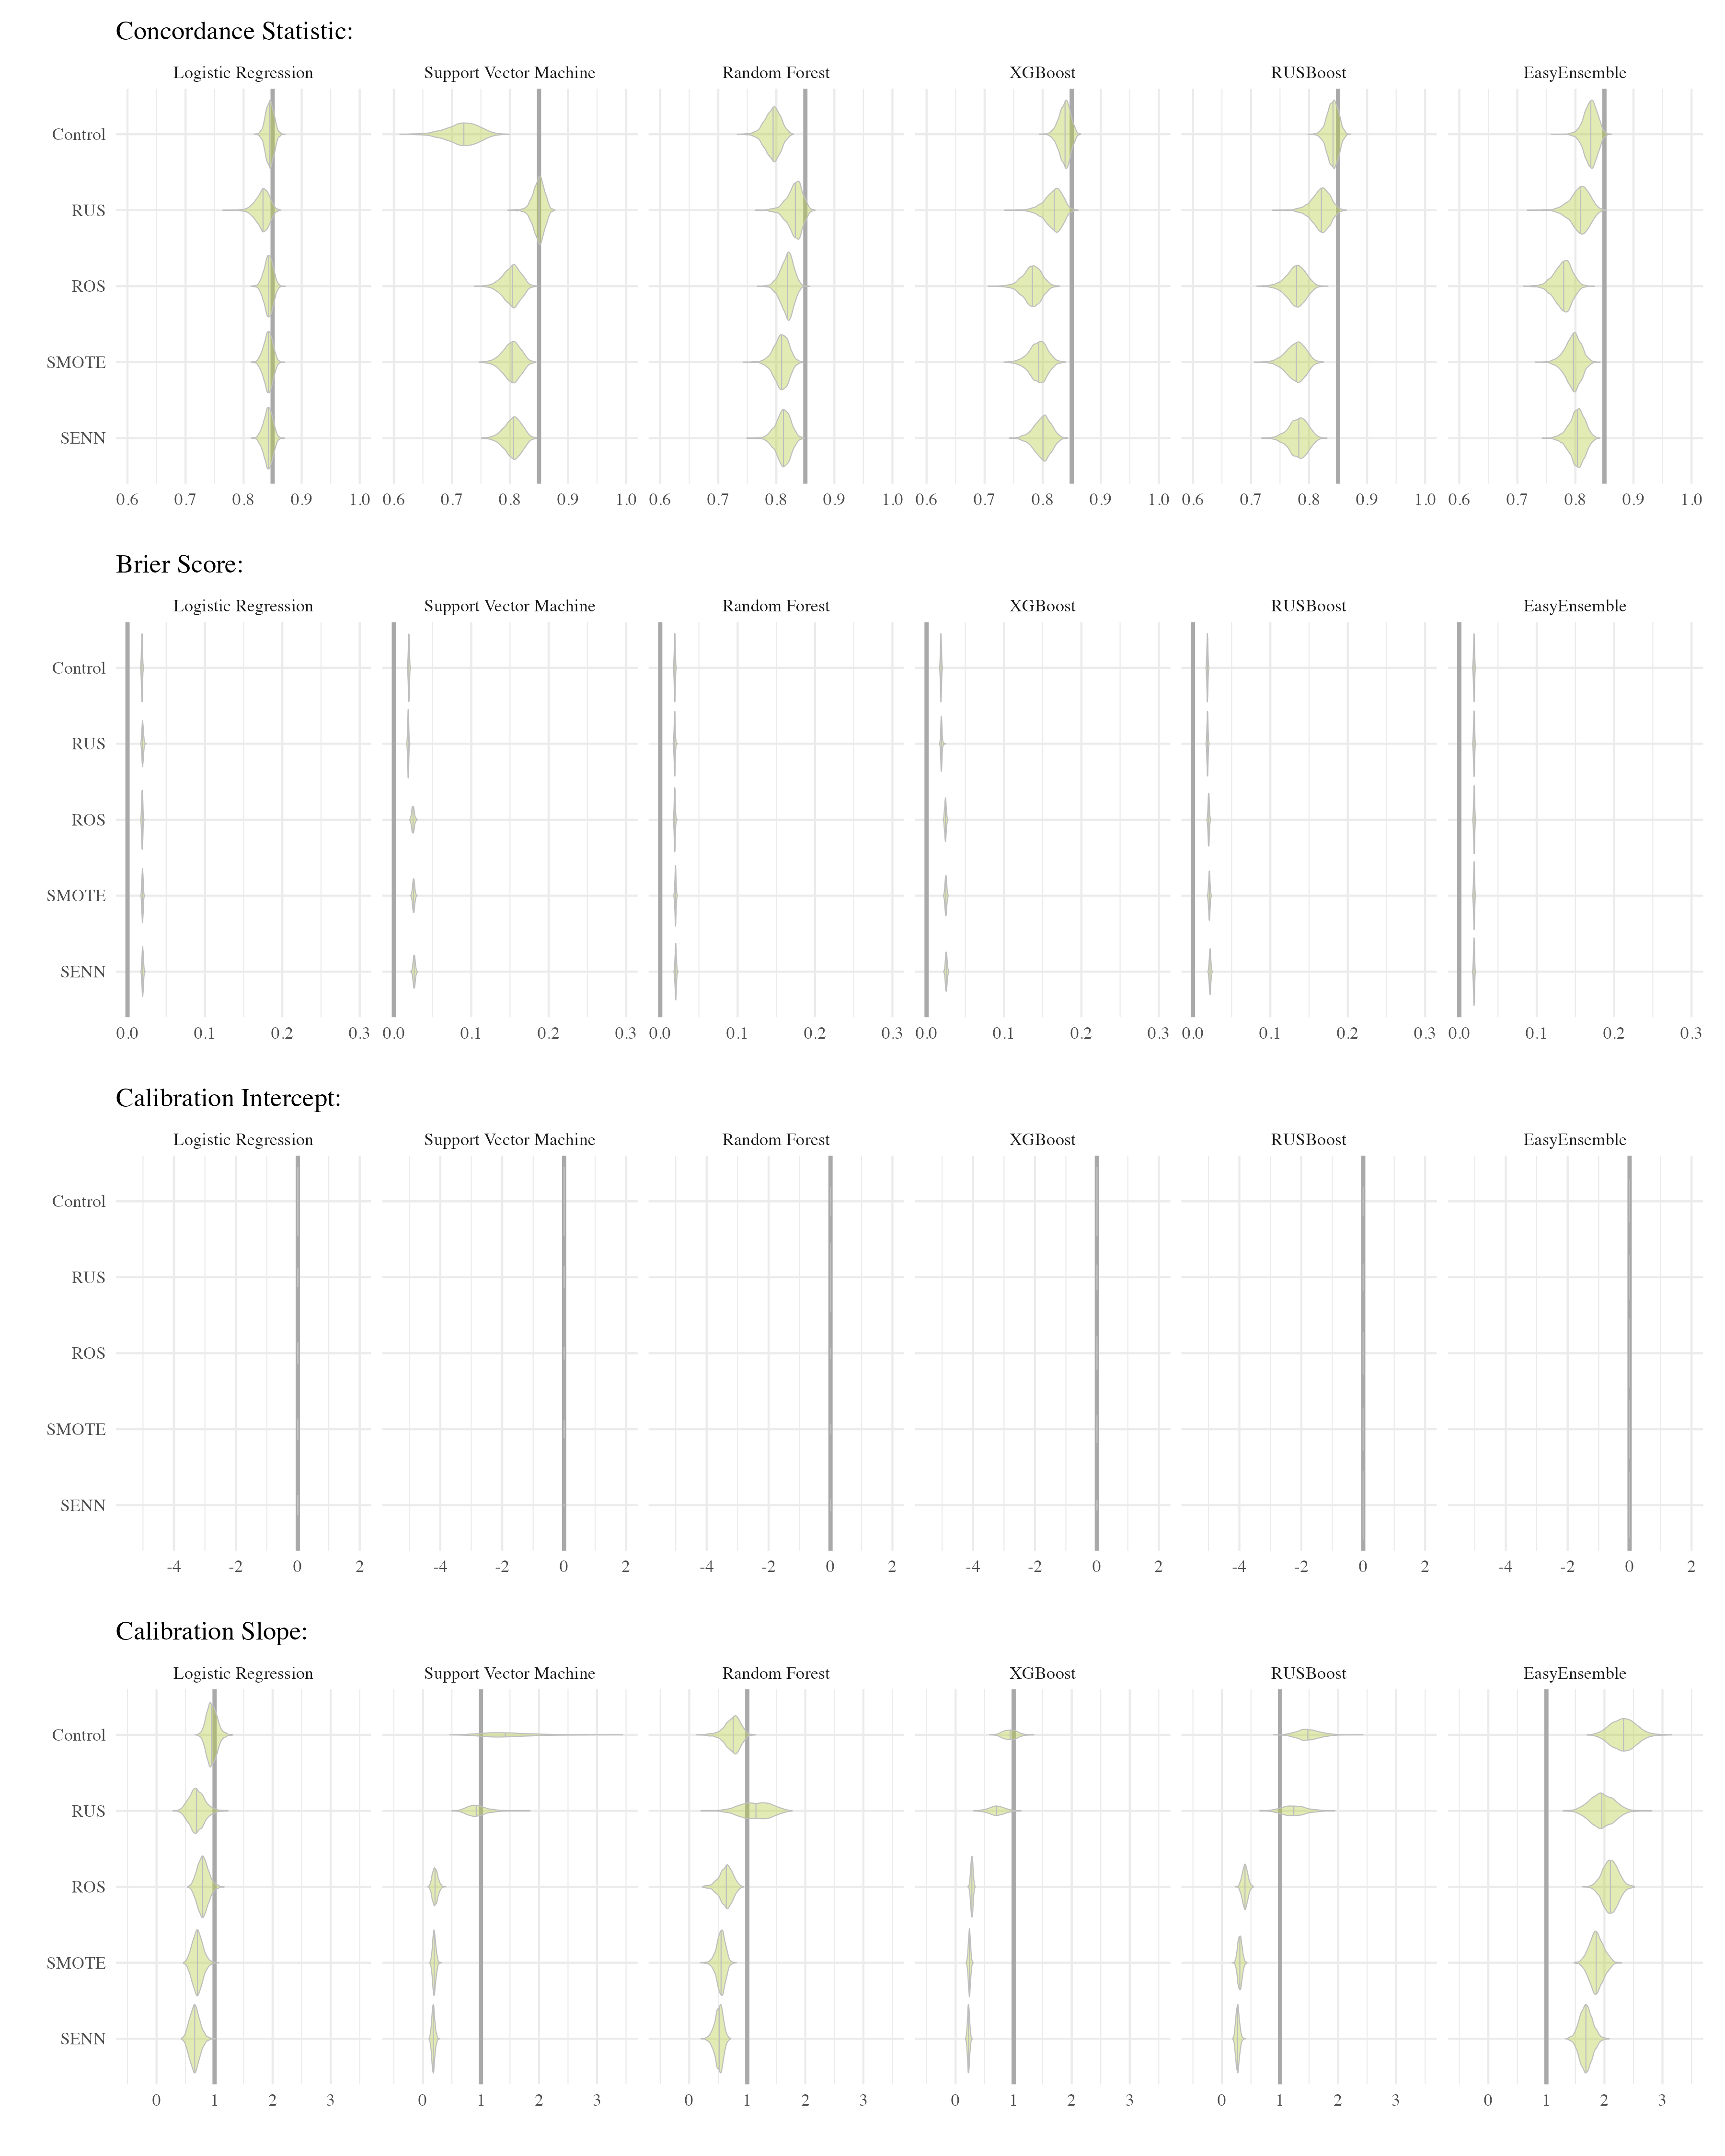
\includegraphics[width=0.7\linewidth]{./figures/performance_metrics_manuscript_sc9_recalibrated} 

}

\caption{Empirical performance metrics for each of 2000 simulation iterations in simulation scenario 9.  This simulation scenario is characterized by 8 predictors, double the required sample size (2N) and strongly imbalanced data (event fraction = 0.02). Empirical performance metrics were computed with re-calibrated predicted risks. The target value highlighted for the concordance statistic reflects the data-generating concordance statstic, 0.85. Imbalance corrections: RUS (random undersampling), ROS (random oversampling), SMOTE (synthetic majority oversampling), SENN (synthetic majority oversampling with Wilson's Edited Nearest Neighbors). Note: after re-calibration, calibration intercepts were essentially zero for every iteration and are therefore not visible on the plot.  \label{fig:recal_violin_9}}\label{fig:unnamed-chunk-65}
\end{figure}

\begin{figure}

{\centering 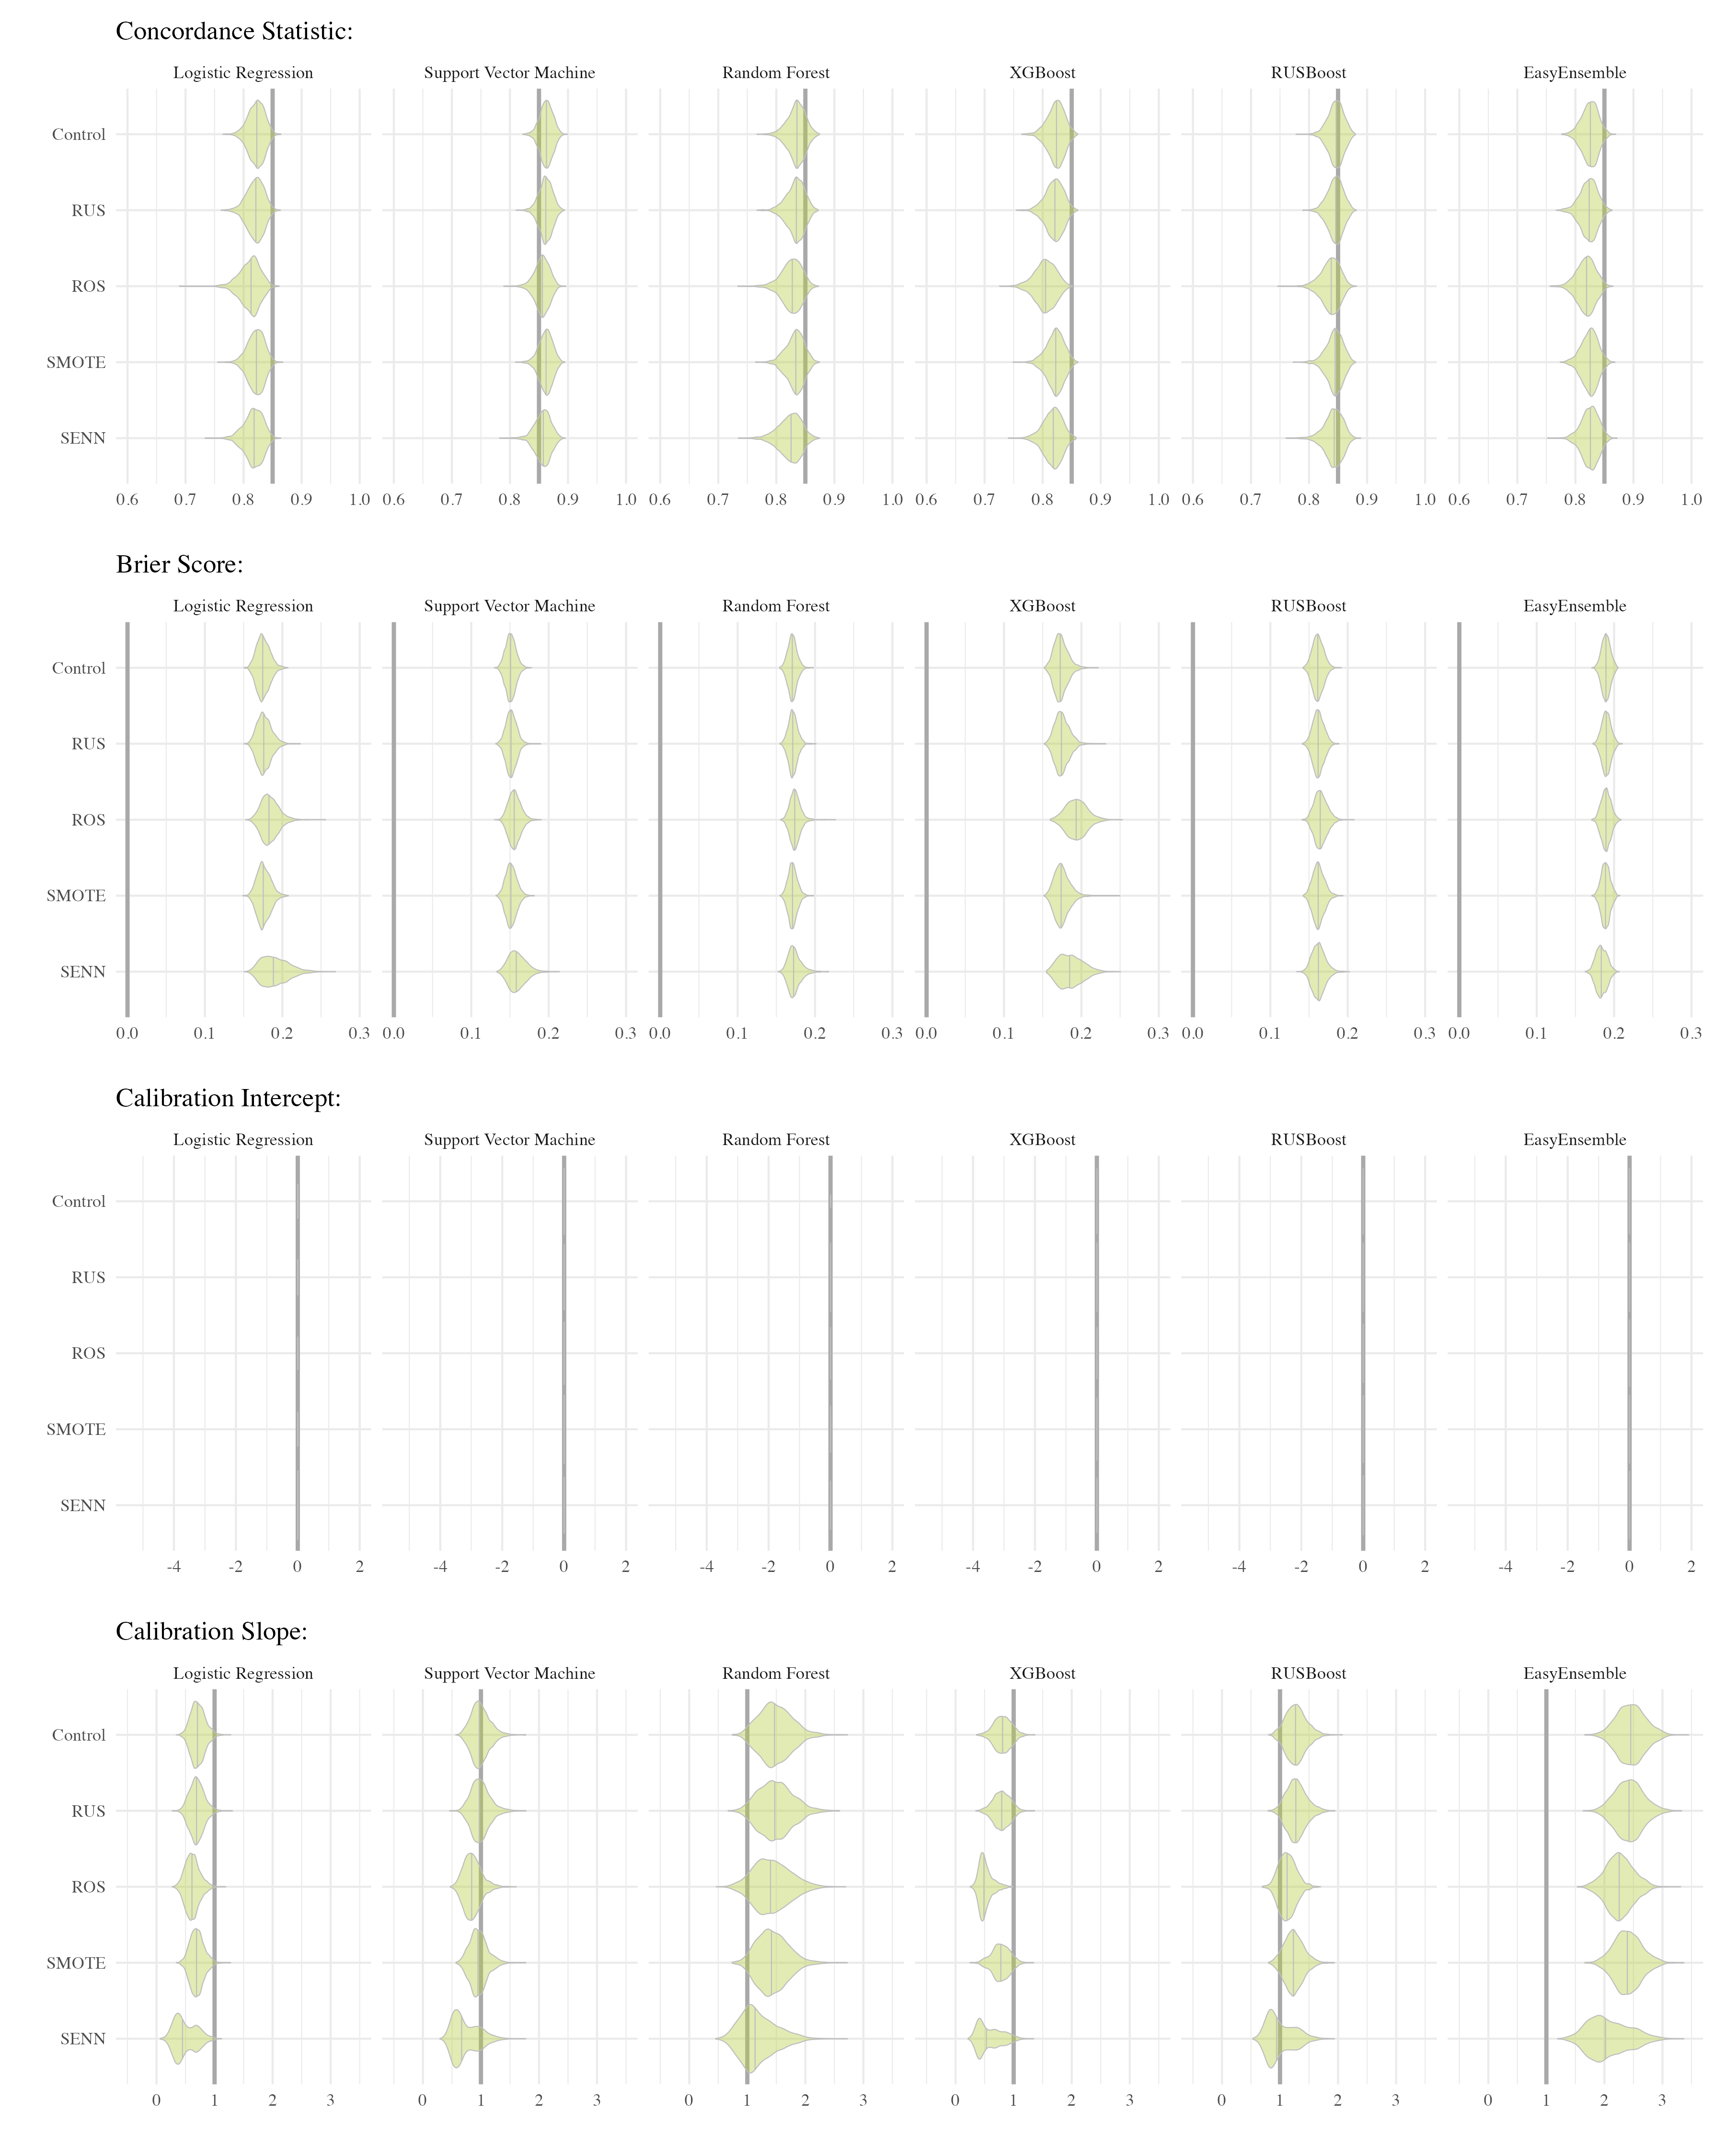
\includegraphics[width=0.7\linewidth]{./figures/performance_metrics_manuscript_sc10_recalibrated} 

}

\caption{Empirical performance metrics for each of 2000 simulation iterations in simulation scenario 10.  This simulation scenario is characterized by 16 predictors, half the required sample size (0.5N) and class balanced data (event fraction = 0.5). Empirical performance metrics were computed with re-calibrated predicted risks. The target value highlighted for the concordance statistic reflects the data-generating concordance statstic, 0.85. Imbalance corrections: RUS (random undersampling), ROS (random oversampling), SMOTE (synthetic majority oversampling), SENN (synthetic majority oversampling with Wilson's Edited Nearest Neighbors). Note: after re-calibration, calibration intercepts were essentially zero for every iteration and are therefore not visible on the plot.  \label{fig:recal_violin_10}}\label{fig:unnamed-chunk-66}
\end{figure}

\begin{figure}

{\centering 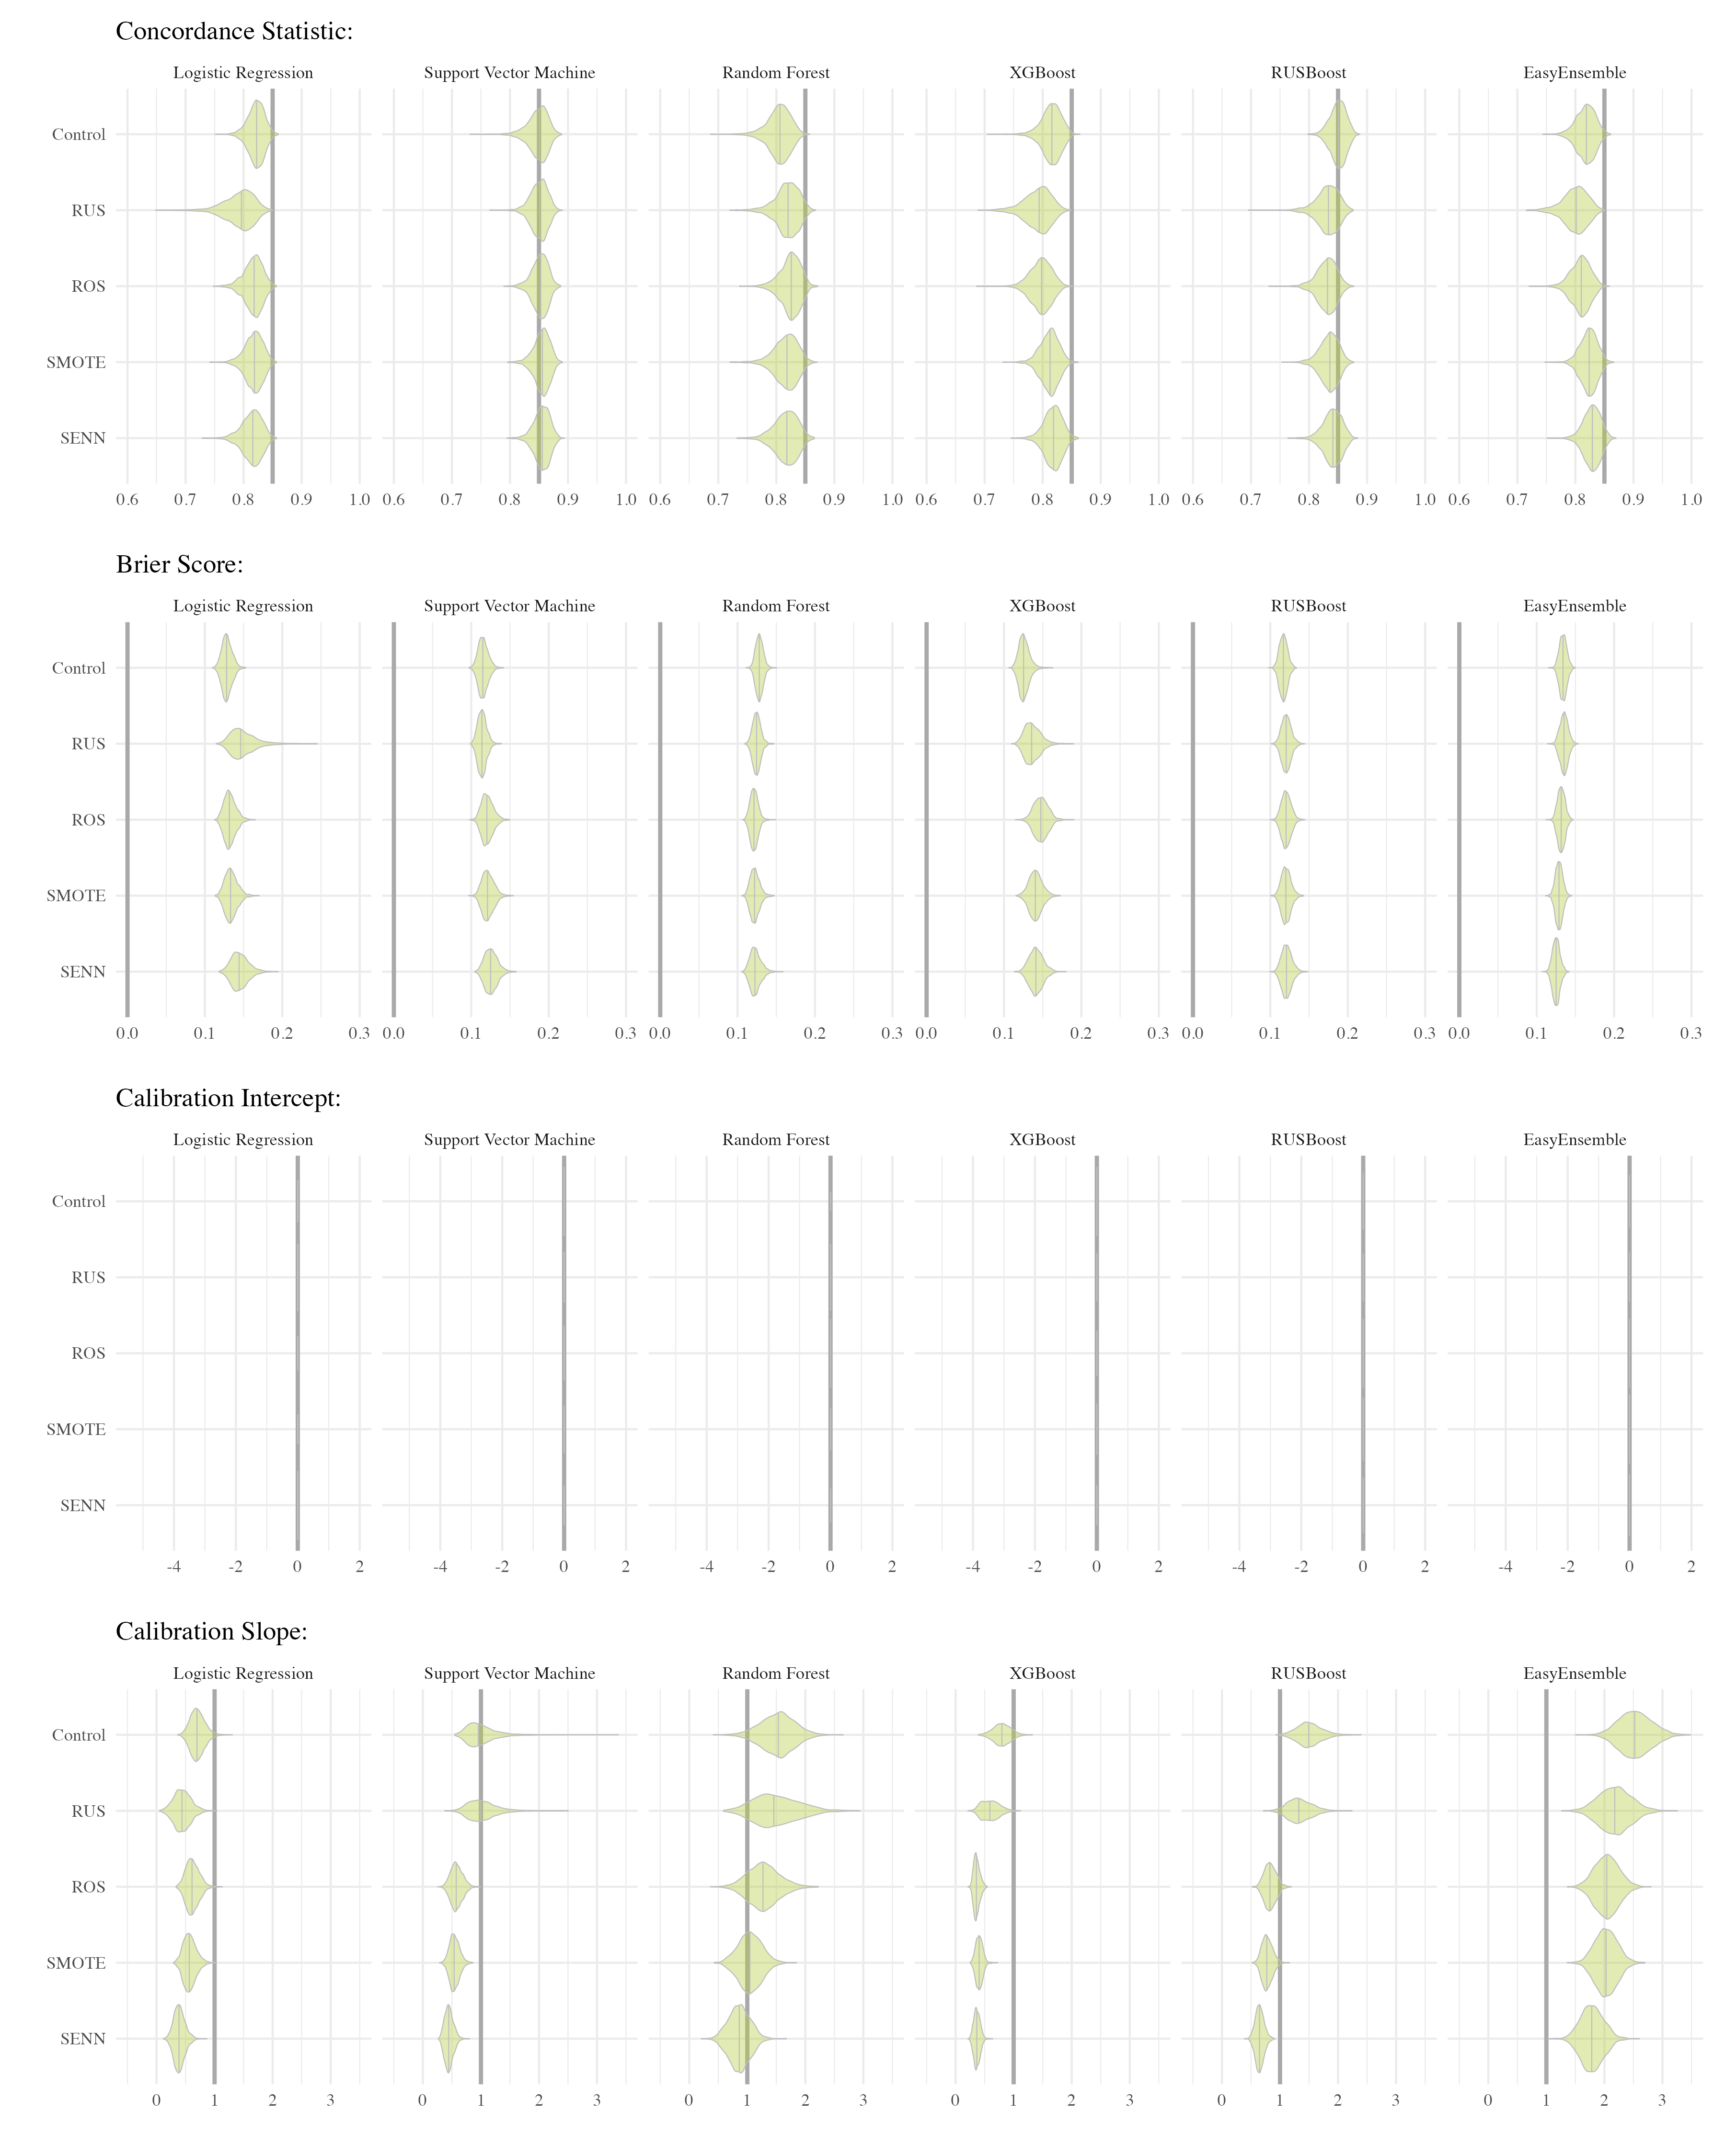
\includegraphics[width=0.7\linewidth]{./figures/performance_metrics_manuscript_sc11_recalibrated} 

}

\caption{Empirical performance metrics for each of 2000 simulation iterations in simulation scenario 11.  This simulation scenario is characterized by 16 predictors, half the required sample size (0.5N) and moderately imbalanced data (event fraction = 0.2). Empirical performance metrics were computed with re-calibrated predicted risks. The target value highlighted for the concordance statistic reflects the data-generating concordance statstic, 0.85. Imbalance corrections: RUS (random undersampling), ROS (random oversampling), SMOTE (synthetic majority oversampling), SENN (synthetic majority oversampling with Wilson's Edited Nearest Neighbors). Note: after re-calibration, calibration intercepts were essentially zero for every iteration and are therefore not visible on the plot.  \label{fig:recal_violin_11}}\label{fig:unnamed-chunk-67}
\end{figure}

\begin{figure}

{\centering 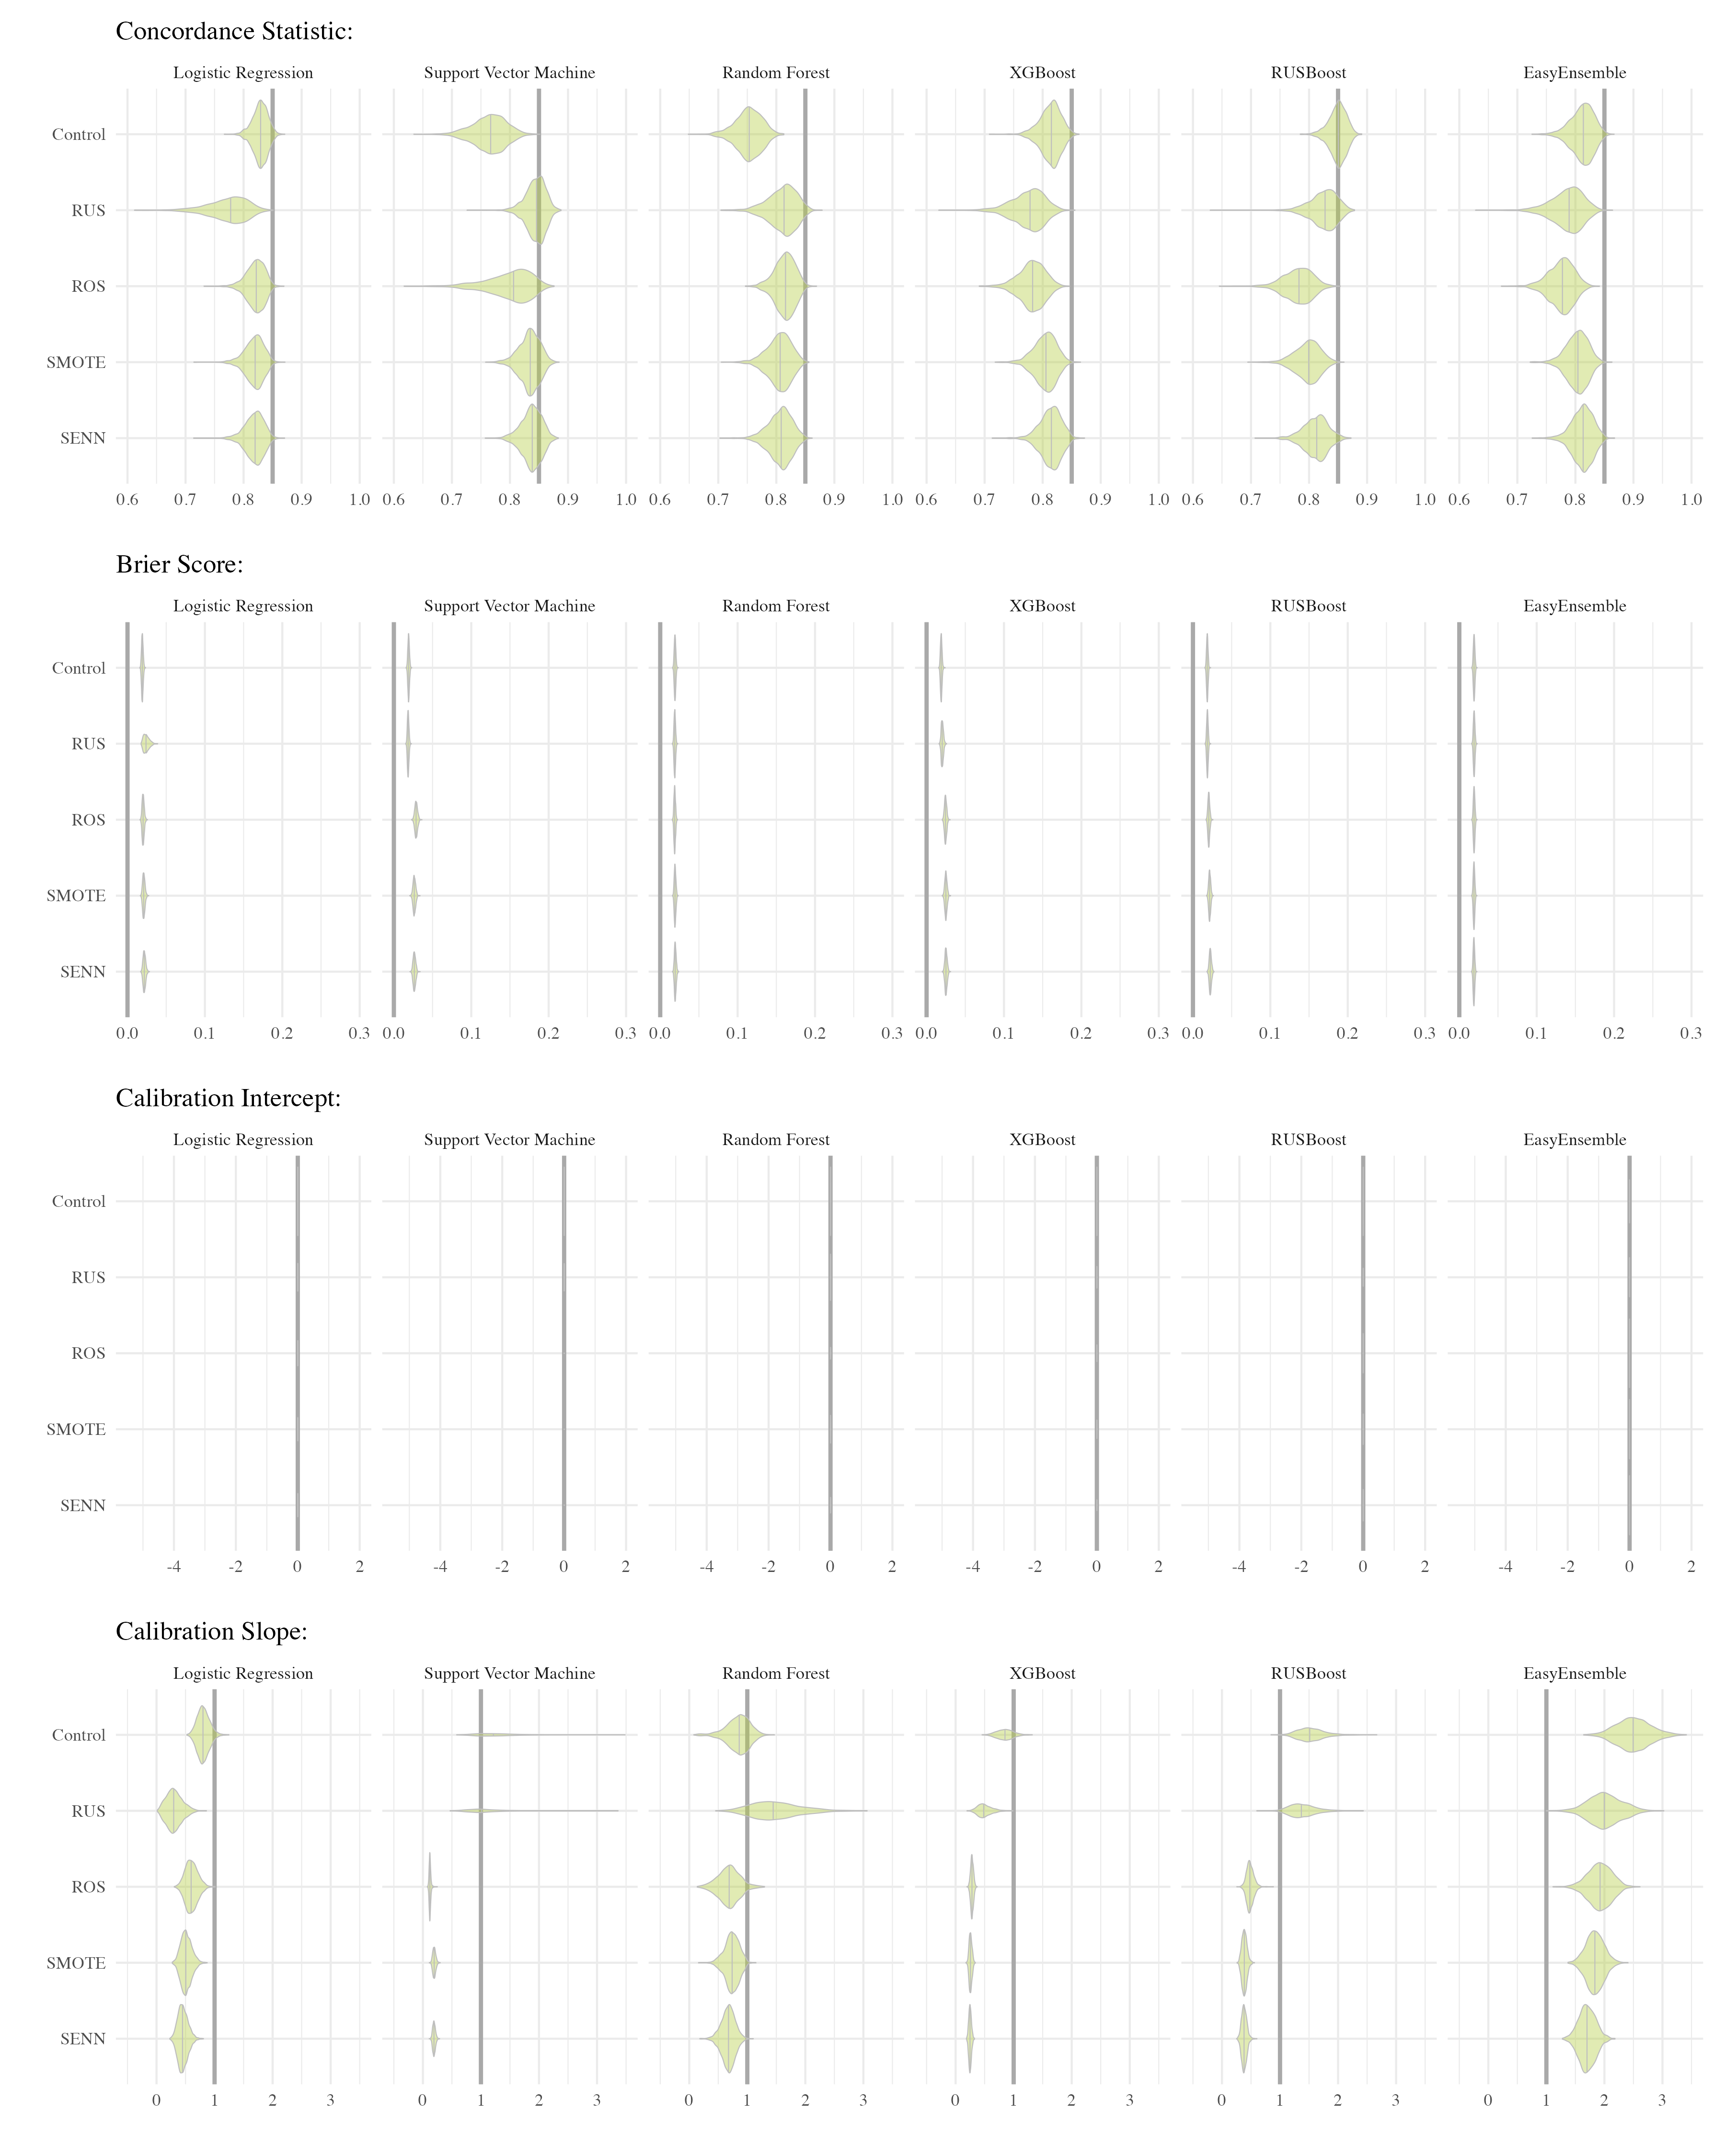
\includegraphics[width=0.7\linewidth]{./figures/performance_metrics_manuscript_sc12_recalibrated} 

}

\caption{Empirical performance metrics for each of 2000 simulation iterations in simulation scenario 12.  This simulation scenario is characterized by 16 predictors, half the required sample size (0.5N) and strongly imbalanced data (event fraction = 0.02). Empirical performance metrics were computed with re-calibrated predicted risks. The target value highlighted for the concordance statistic reflects the data-generating concordance statstic, 0.85. Imbalance corrections: RUS (random undersampling), ROS (random oversampling), SMOTE (synthetic majority oversampling), SENN (synthetic majority oversampling with Wilson's Edited Nearest Neighbors). Note: after re-calibration, calibration intercepts were essentially zero for every iteration and are therefore not visible on the plot.  \label{fig:recal_violin_12}}\label{fig:unnamed-chunk-68}
\end{figure}

\begin{figure}

{\centering 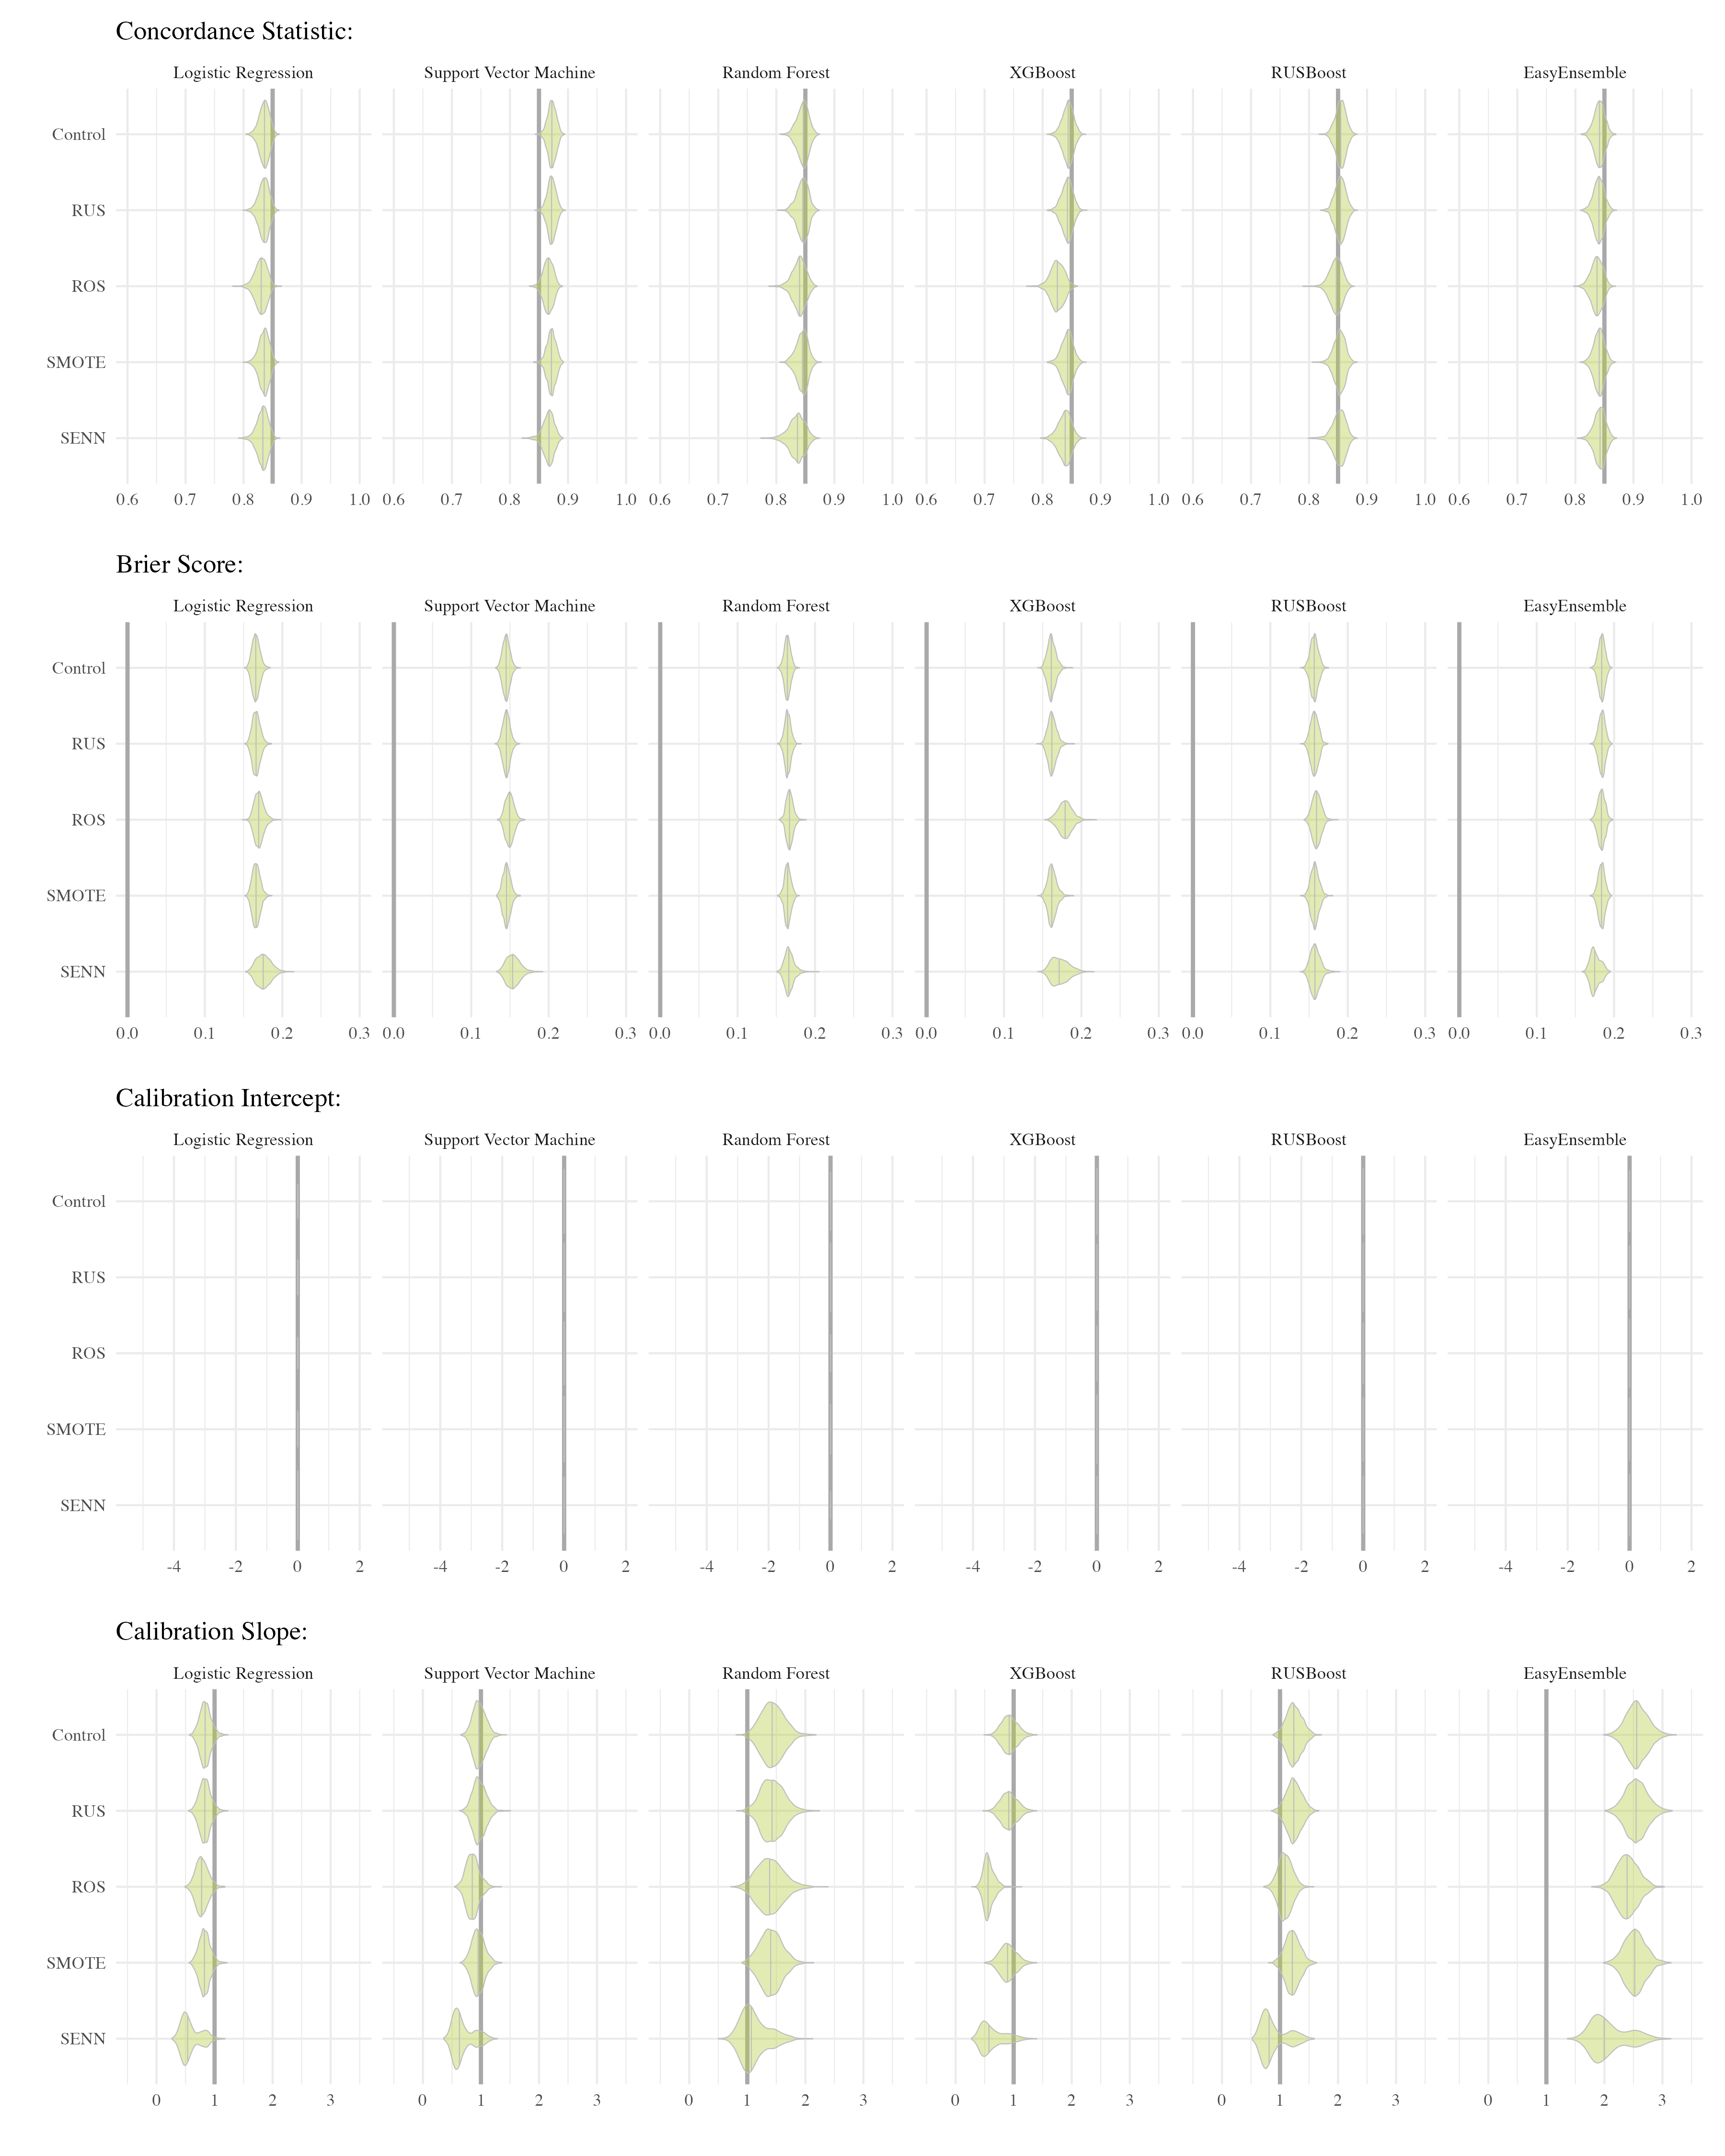
\includegraphics[width=0.7\linewidth]{./figures/performance_metrics_manuscript_sc13_recalibrated} 

}

\caption{Empirical performance metrics for each of 2000 simulation iterations in simulation scenario 13.  This simulation scenario is characterized by 16 predictors, minimum required sample size (N) and class balanced data (event fraction = 0.5). Empirical performance metrics were computed with re-calibrated predicted risks. The target value highlighted for the concordance statistic reflects the data-generating concordance statstic, 0.85. Imbalance corrections: RUS (random undersampling), ROS (random oversampling), SMOTE (synthetic majority oversampling), SENN (synthetic majority oversampling with Wilson's Edited Nearest Neighbors). Note: after re-calibration, calibration intercepts were essentially zero for every iteration and are therefore not visible on the plot.  \label{fig:rrecal_violin_13}}\label{fig:unnamed-chunk-69}
\end{figure}

\begin{figure}

{\centering 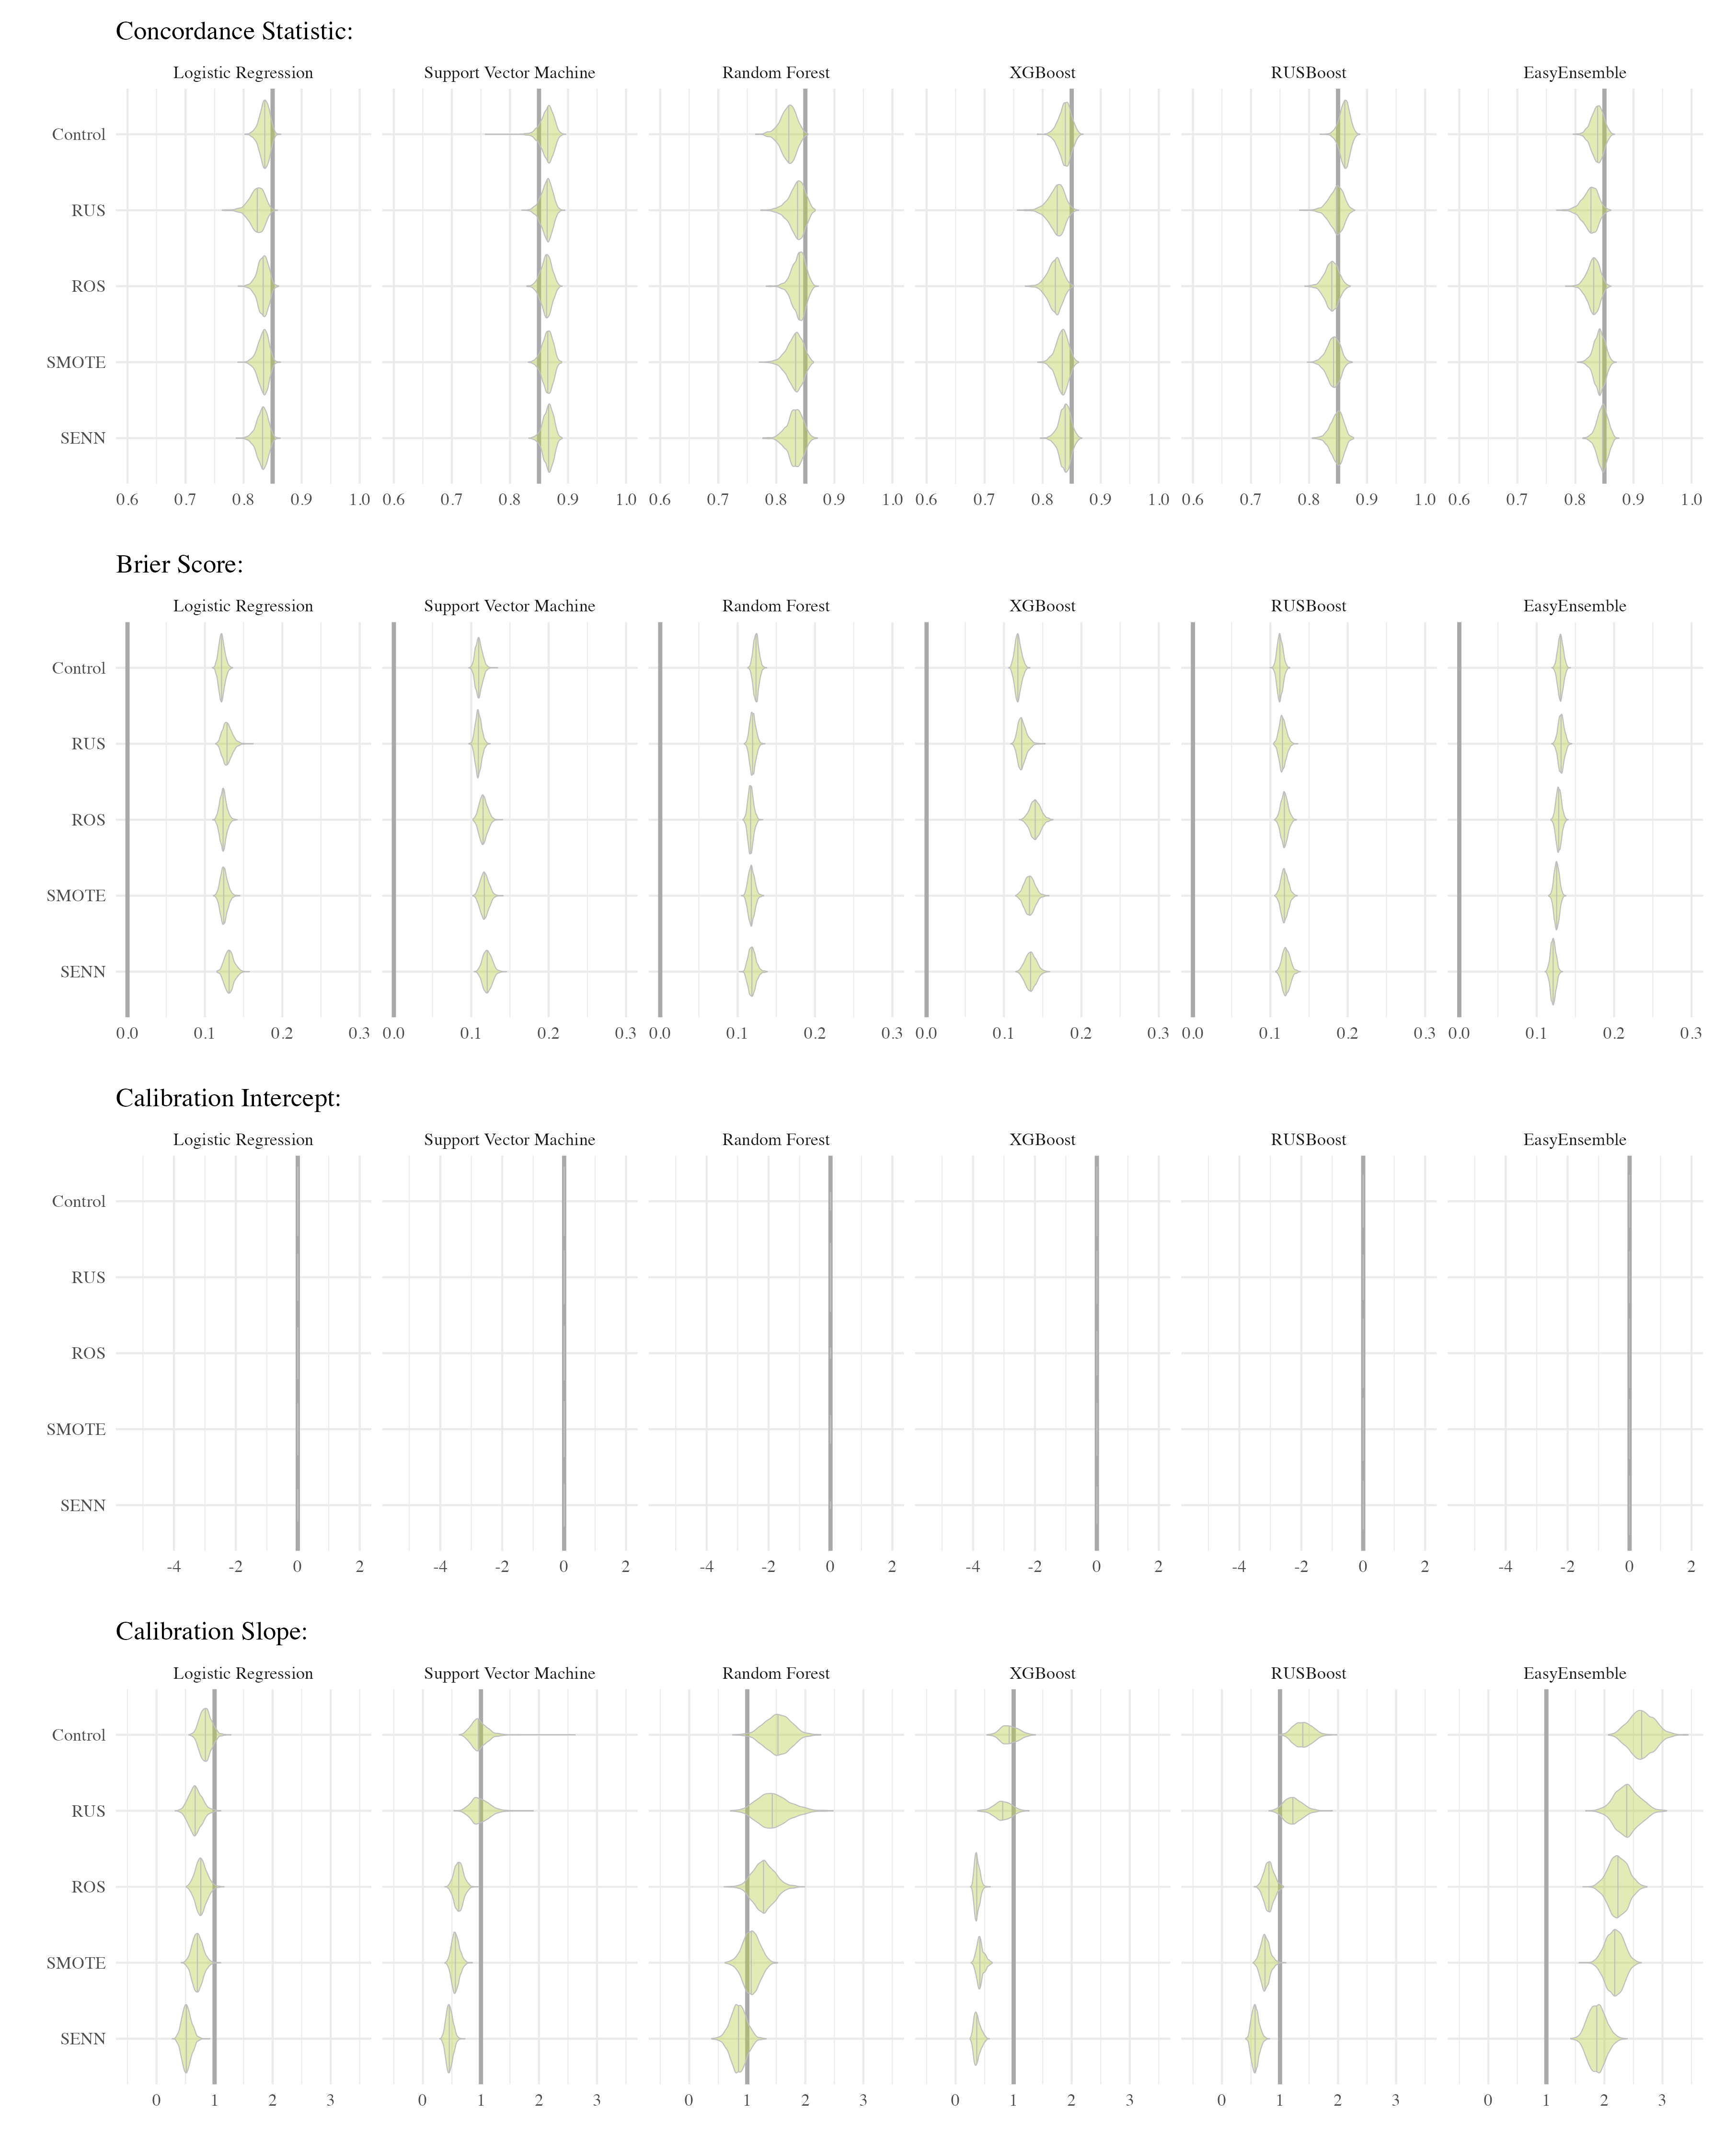
\includegraphics[width=0.7\linewidth]{./figures/performance_metrics_manuscript_sc14_recalibrated} 

}

\caption{Empirical performance metrics for each of 2000 simulation iterations in simulation scenario 14.  This simulation scenario is characterized by 16 predictors, minimum required sample size (N) and moderately imbalanced data (event fraction = 0.2). Empirical performance metrics were computed with re-calibrated predicted risks. The target value highlighted for the concordance statistic reflects the data-generating concordance statstic, 0.85. Imbalance corrections: RUS (random undersampling), ROS (random oversampling), SMOTE (synthetic majority oversampling), SENN (synthetic majority oversampling with Wilson's Edited Nearest Neighbors). Note: after re-calibration, calibration intercepts were essentially zero for every iteration and are therefore not visible on the plot.  \label{fig:recal_violin_14}}\label{fig:unnamed-chunk-70}
\end{figure}

\begin{figure}

{\centering 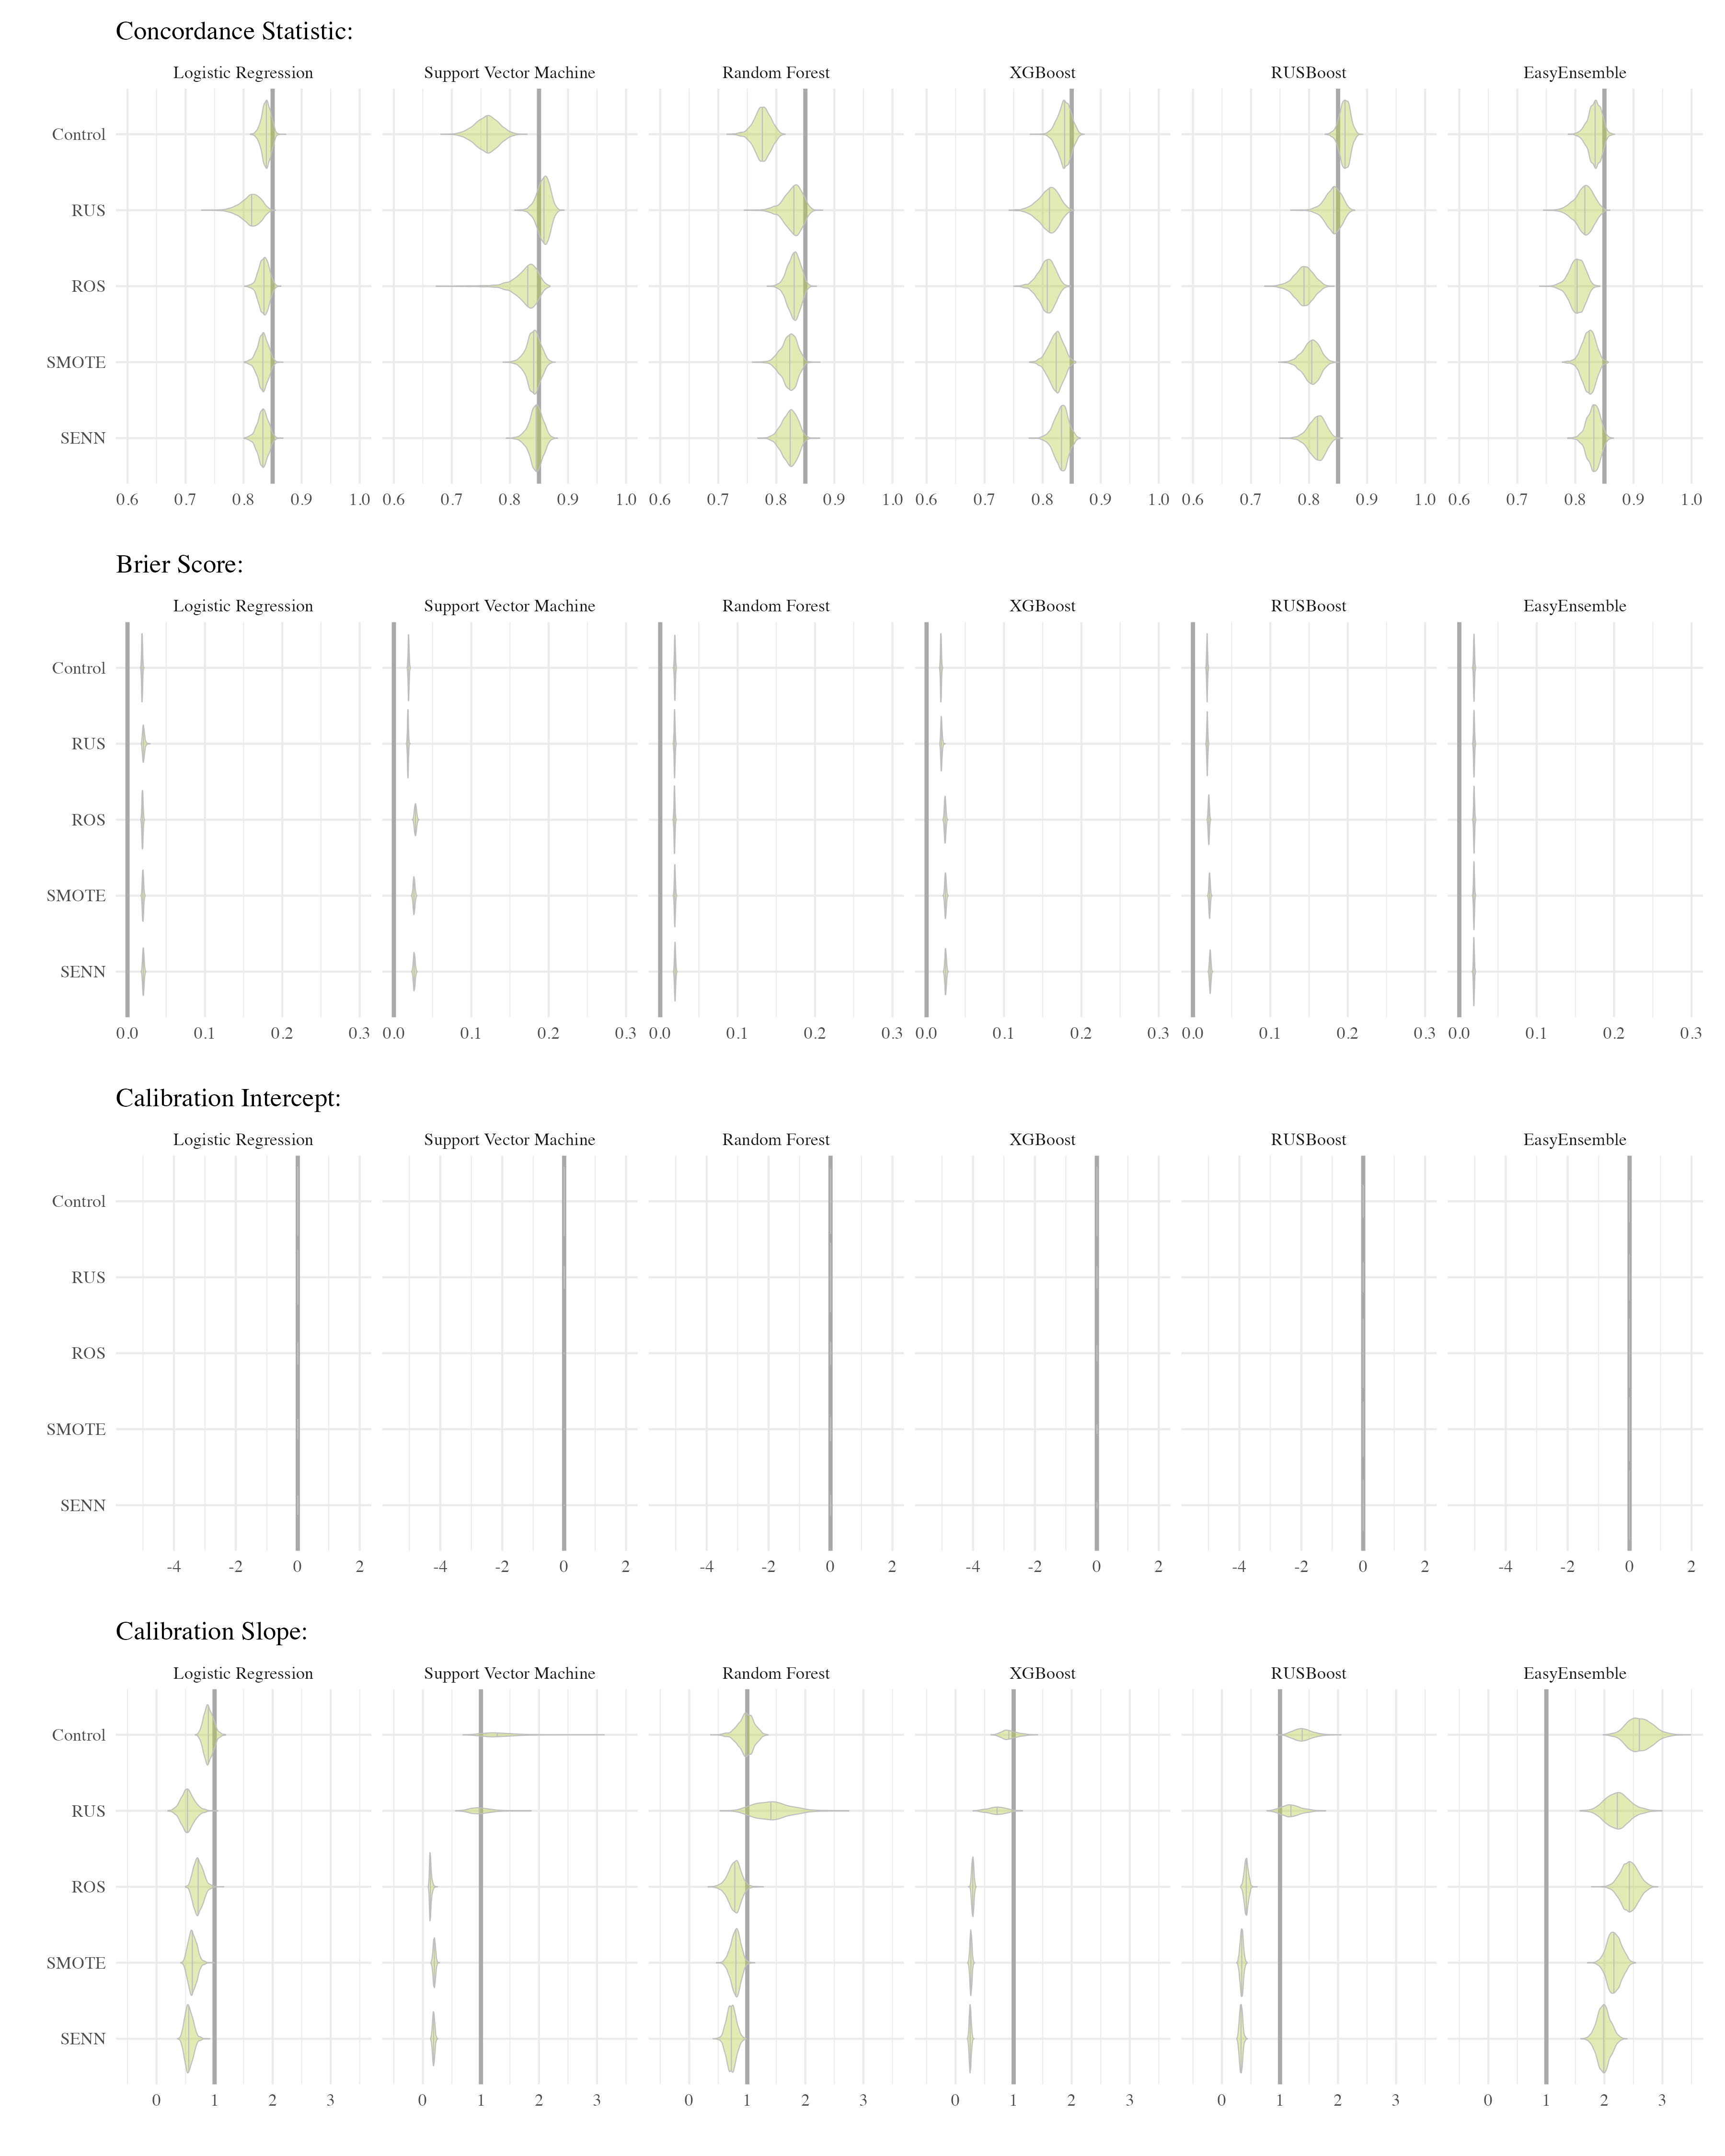
\includegraphics[width=0.7\linewidth]{./figures/performance_metrics_manuscript_sc15_recalibrated} 

}

\caption{Empirical performance metrics for each of 2000 simulation iterations in simulation scenario 15.  This simulation scenario is characterized by 16 predictors, minimum required sample size (N) and strongly imbalanced data (event fraction = 0.02). Empirical performance metrics were computed with re-calibrated predicted risks. The target value highlighted for the concordance statistic reflects the data-generating concordance statstic, 0.85. Imbalance corrections: RUS (random undersampling), ROS (random oversampling), SMOTE (synthetic majority oversampling), SENN (synthetic majority oversampling with Wilson's Edited Nearest Neighbors). Note: after re-calibration, calibration intercepts were essentially zero for every iteration and are therefore not visible on the plot.  \label{fig:recal_violin_15}}\label{fig:unnamed-chunk-71}
\end{figure}

\begin{figure}

{\centering 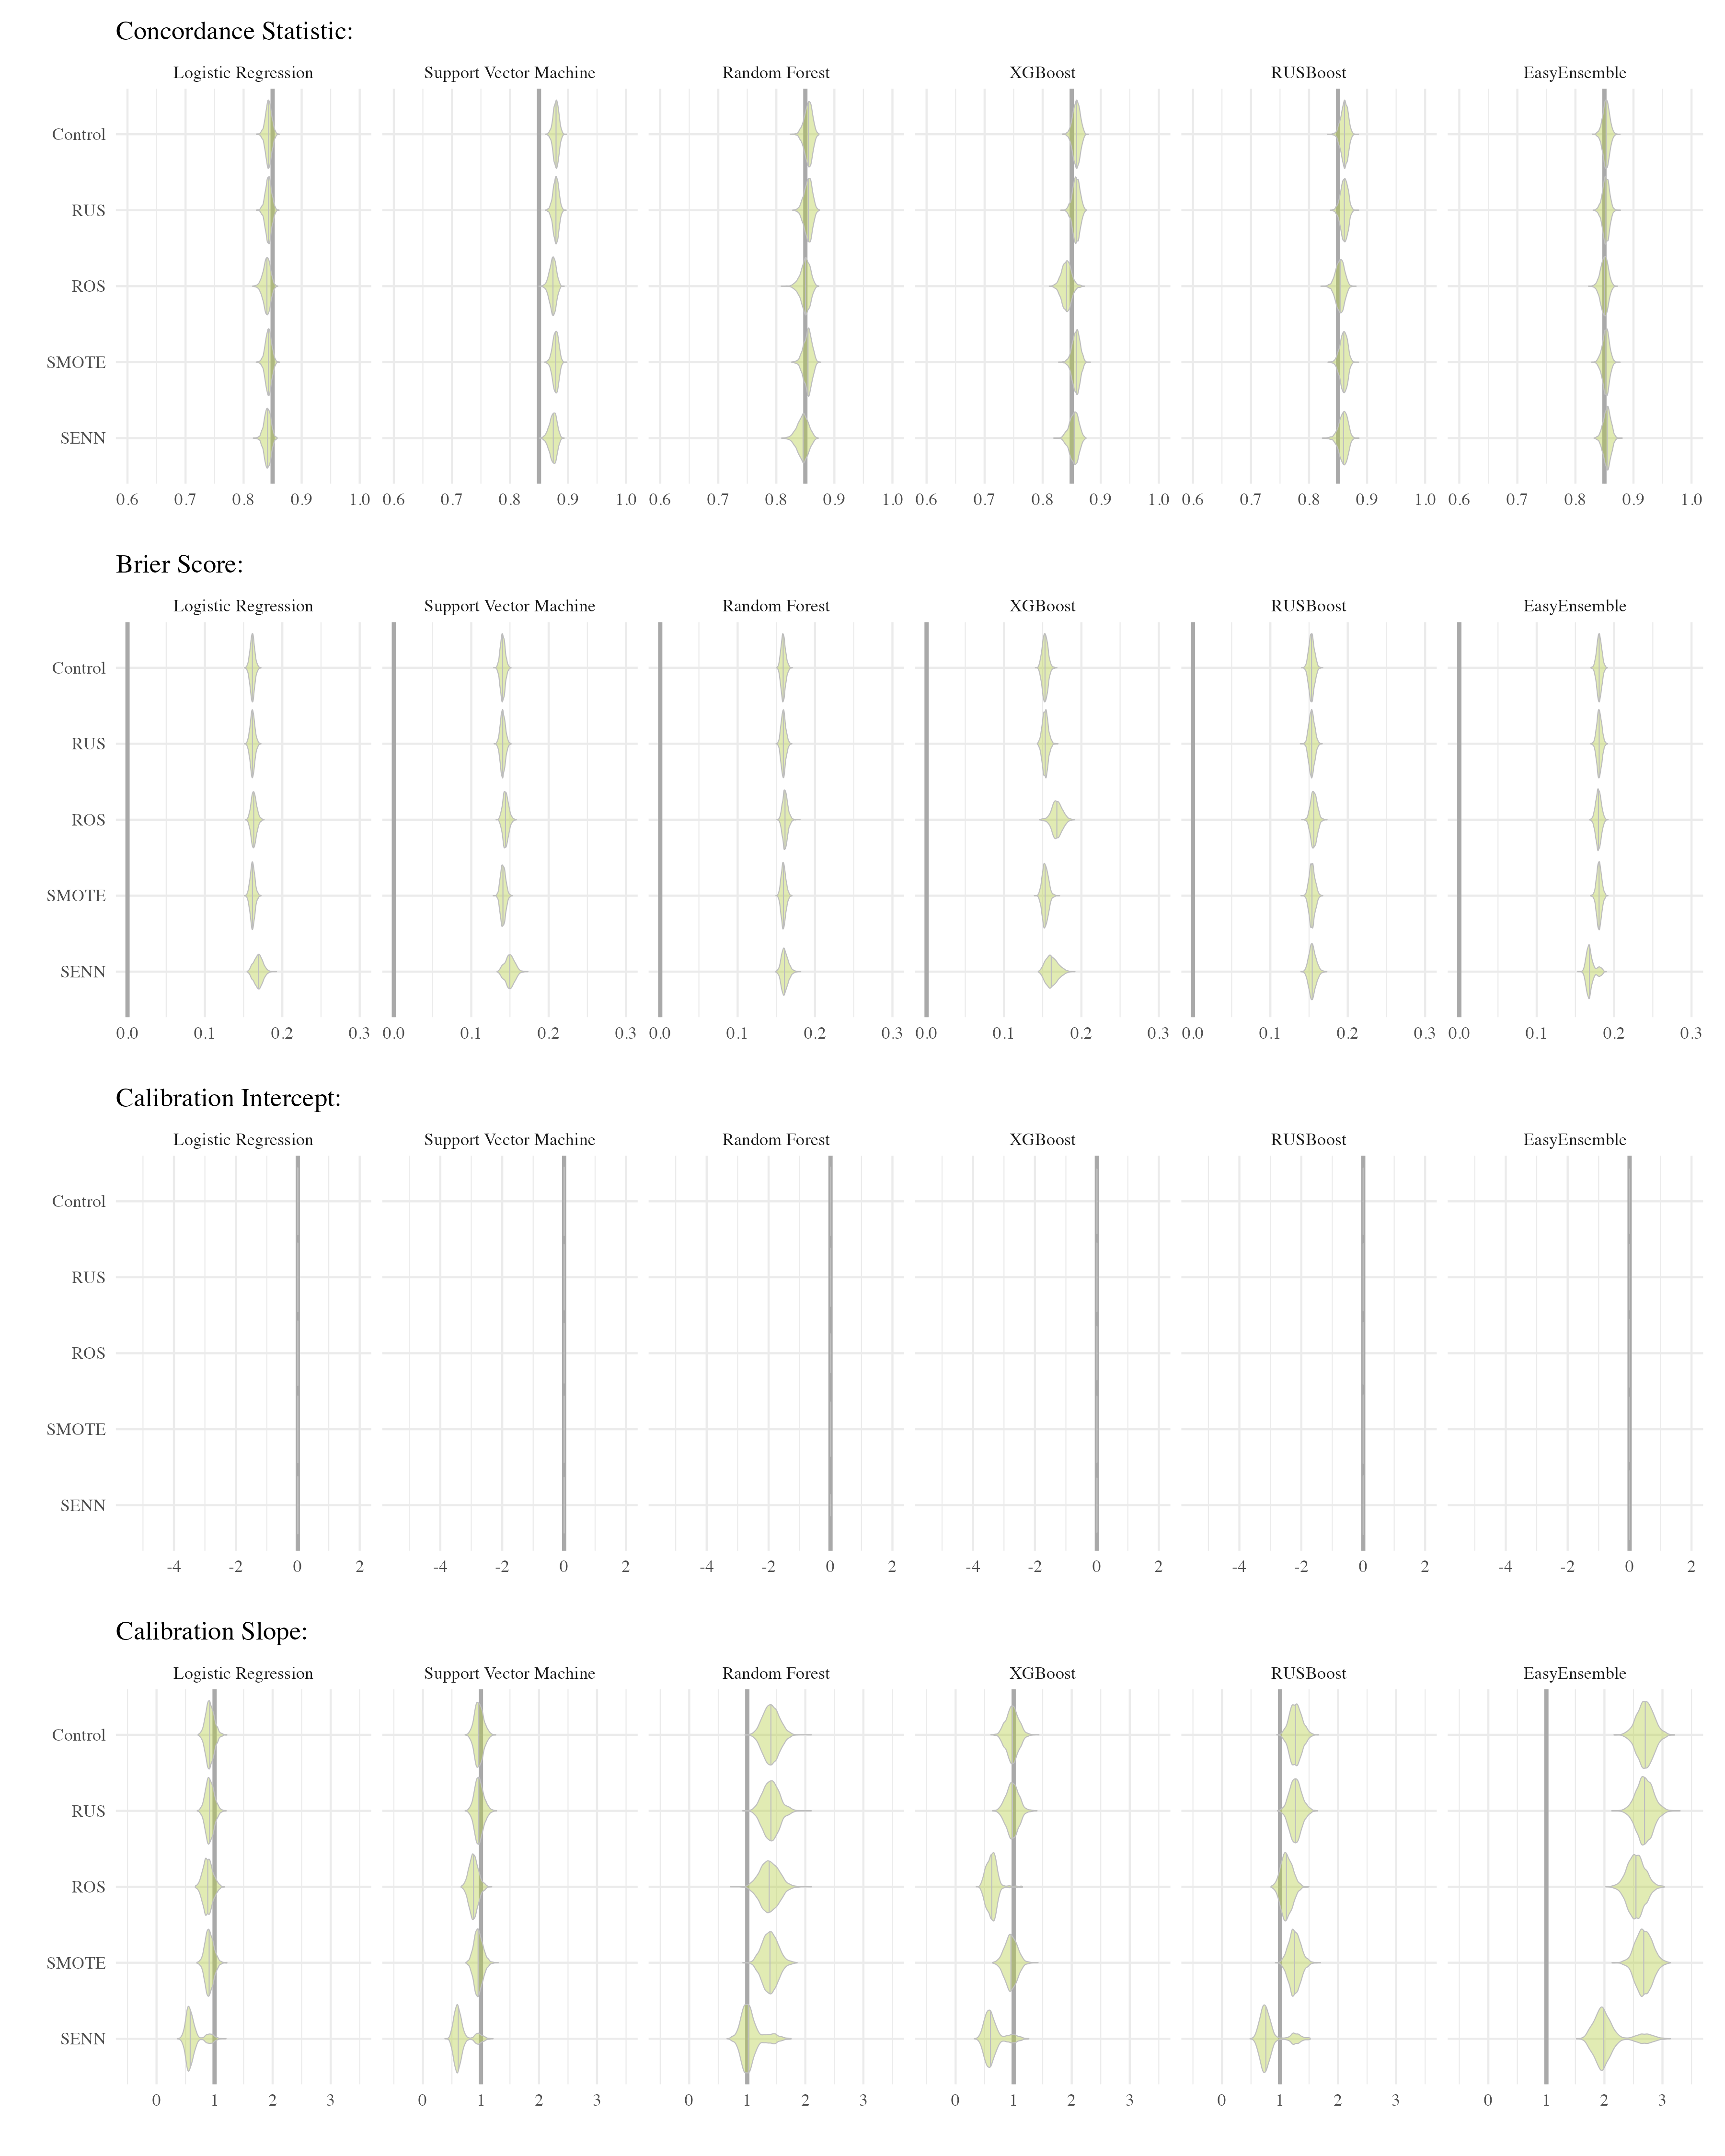
\includegraphics[width=0.7\linewidth]{./figures/performance_metrics_manuscript_sc16_recalibrated} 

}

\caption{Empirical performance metrics for each of 2000 simulation iterations in simulation scenario 16.  This simulation scenario is characterized by 16 predictors, double the required sample size (2N) and class balanced data (event fraction = 0.5). Empirical performance metrics were computed with re-calibrated predicted risks. The target value highlighted for the concordance statistic reflects the data-generating concordance statstic, 0.85. Imbalance corrections: RUS (random undersampling), ROS (random oversampling), SMOTE (synthetic majority oversampling), SENN (synthetic majority oversampling with Wilson's Edited Nearest Neighbors). Note: after re-calibration, calibration intercepts were essentially zero for every iteration and are therefore not visible on the plot.  \label{fig:recal_violin_16}}\label{fig:unnamed-chunk-72}
\end{figure}

\begin{figure}

{\centering 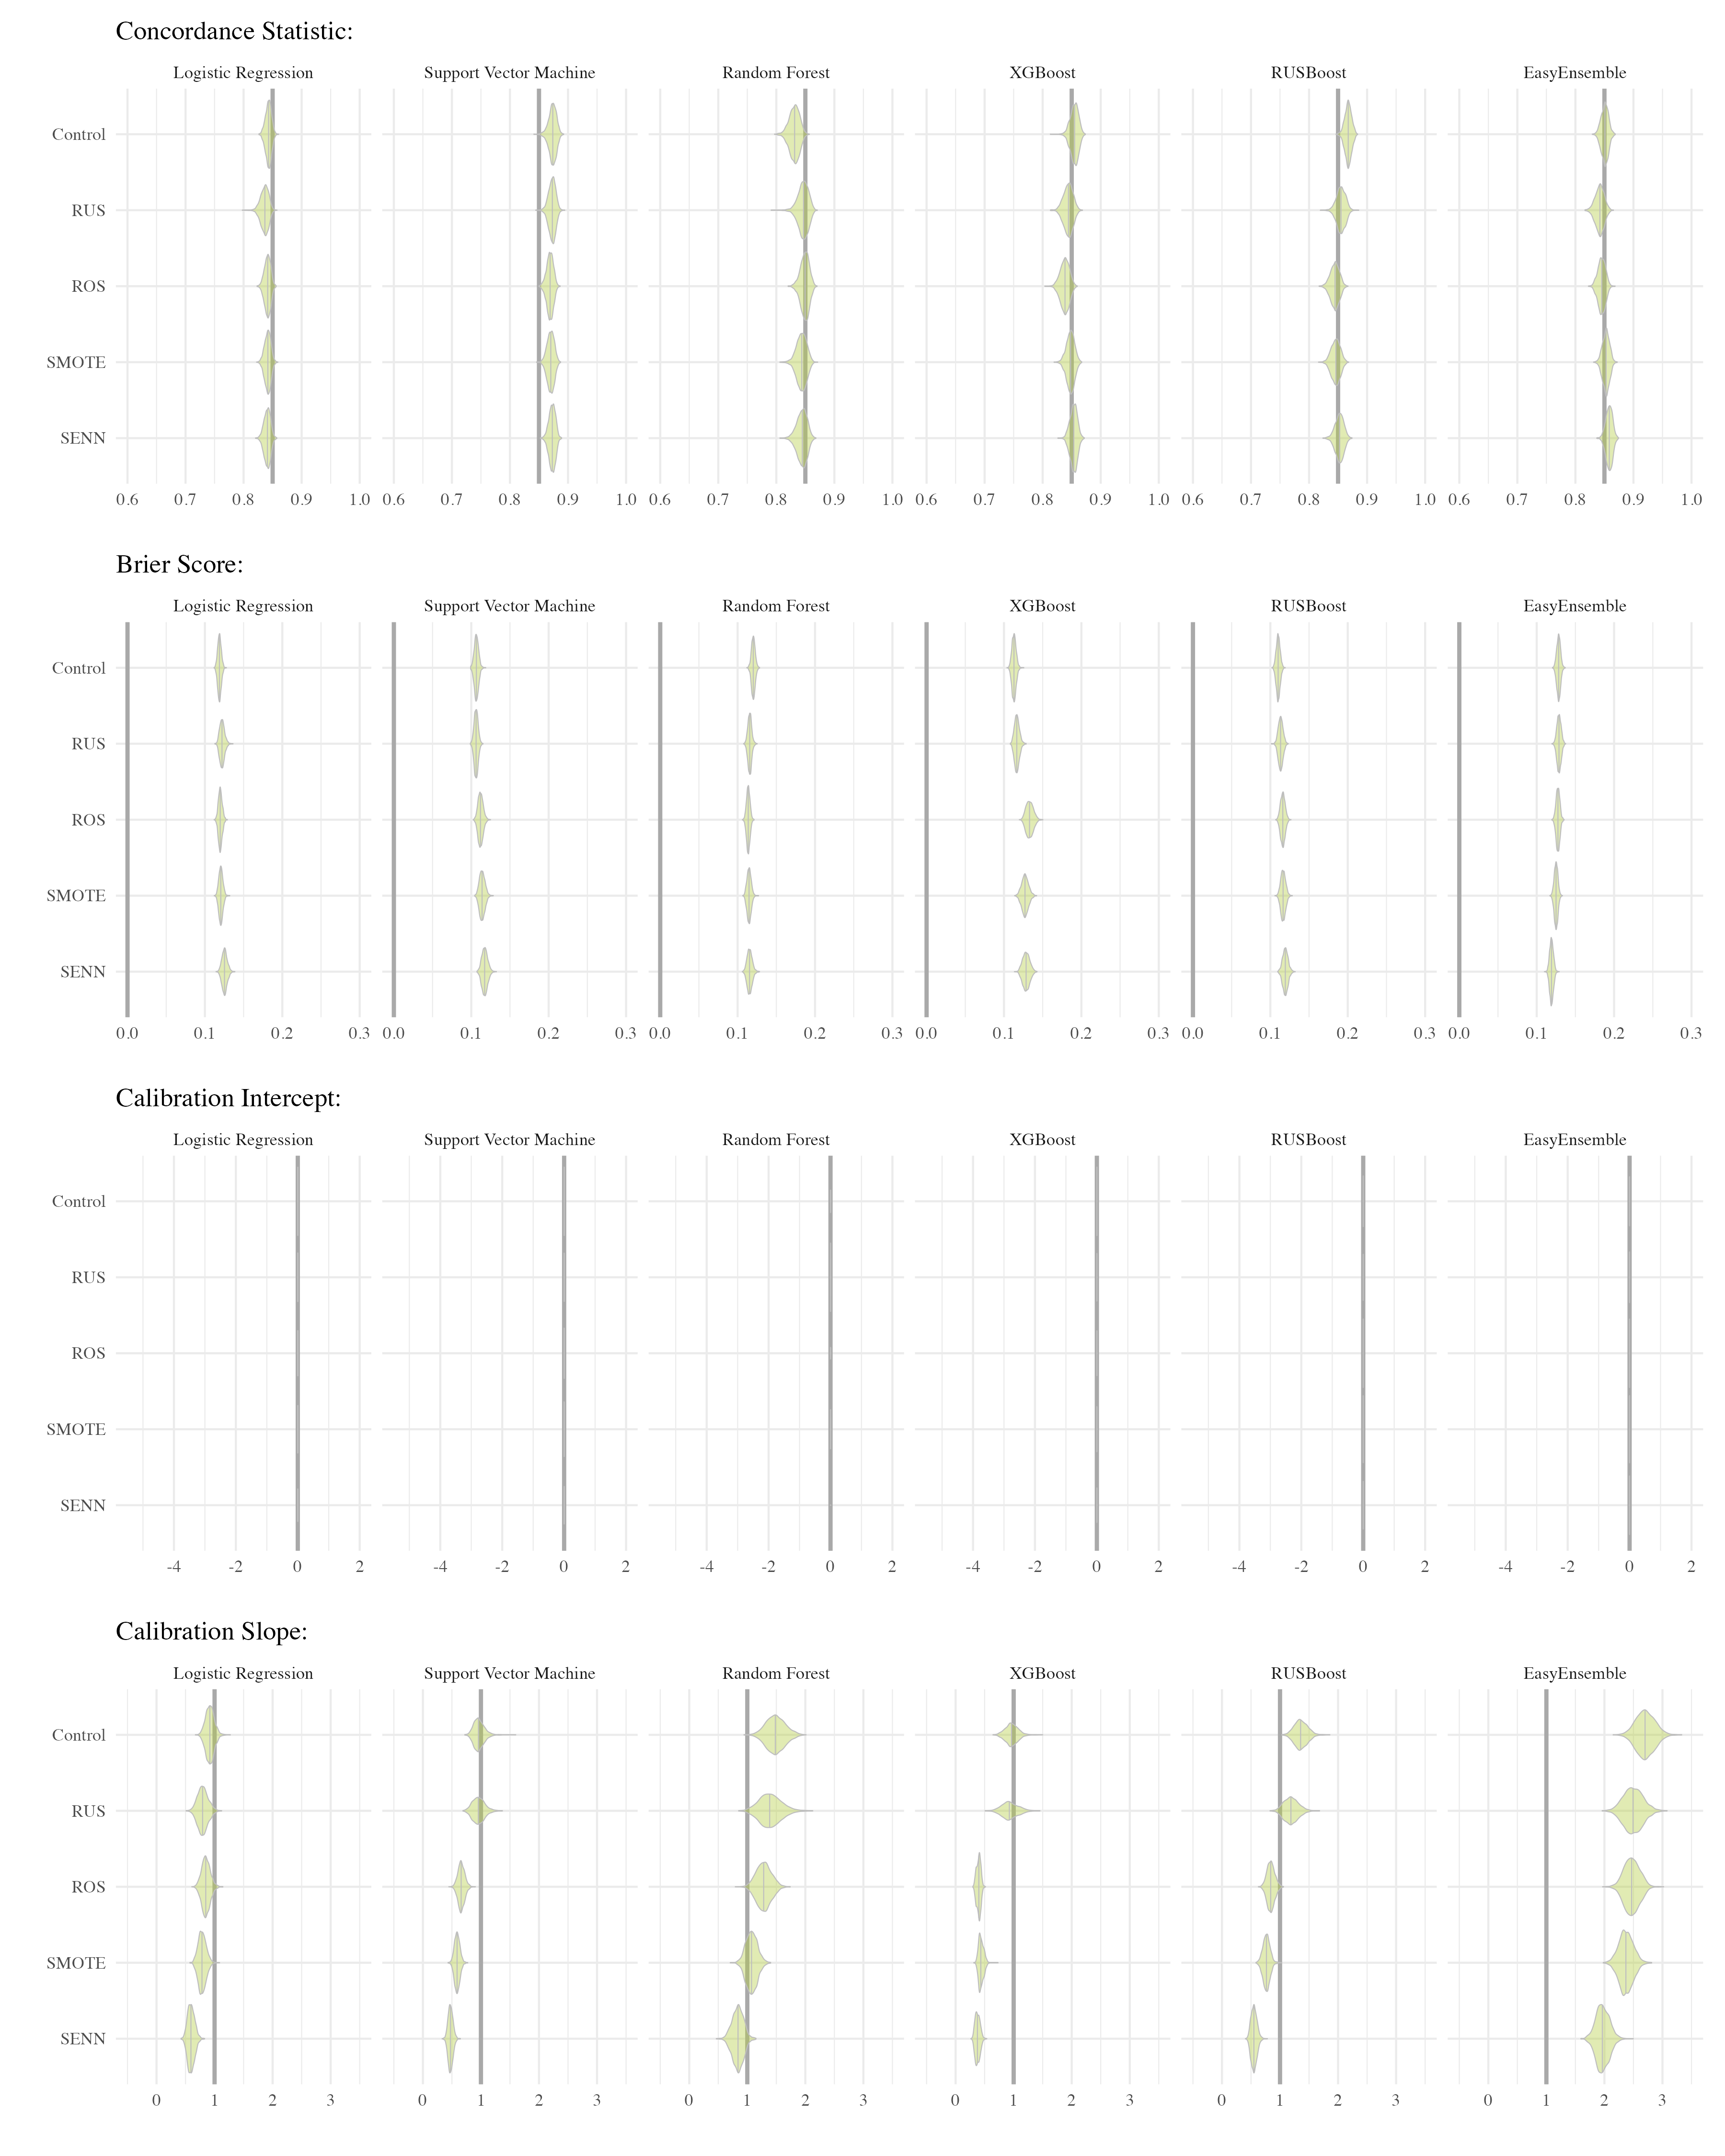
\includegraphics[width=0.7\linewidth]{./figures/performance_metrics_manuscript_sc17_recalibrated} 

}

\caption{Empirical performance metrics for each of 2000 simulation iterations in simulation scenario 17.  This simulation scenario is characterized by 16 predictors, double the required sample size (2N) and moderately imbalanced data (event fraction = 0.2). Empirical performance metrics were computed with re-calibrated predicted risks.  The target value highlighted for the concordance statistic reflects the data-generating concordance statstic, 0.85. Imbalance corrections: RUS (random undersampling), ROS (random oversampling), SMOTE (synthetic majority oversampling), SENN (synthetic majority oversampling with Wilson's Edited Nearest Neighbors). Note: after re-calibration, calibration intercepts were essentially zero for every iteration and are therefore not visible on the plot.  \label{fig:recal_violin_17}}\label{fig:unnamed-chunk-73}
\end{figure}
\clearpage
\begin{figure}

{\centering 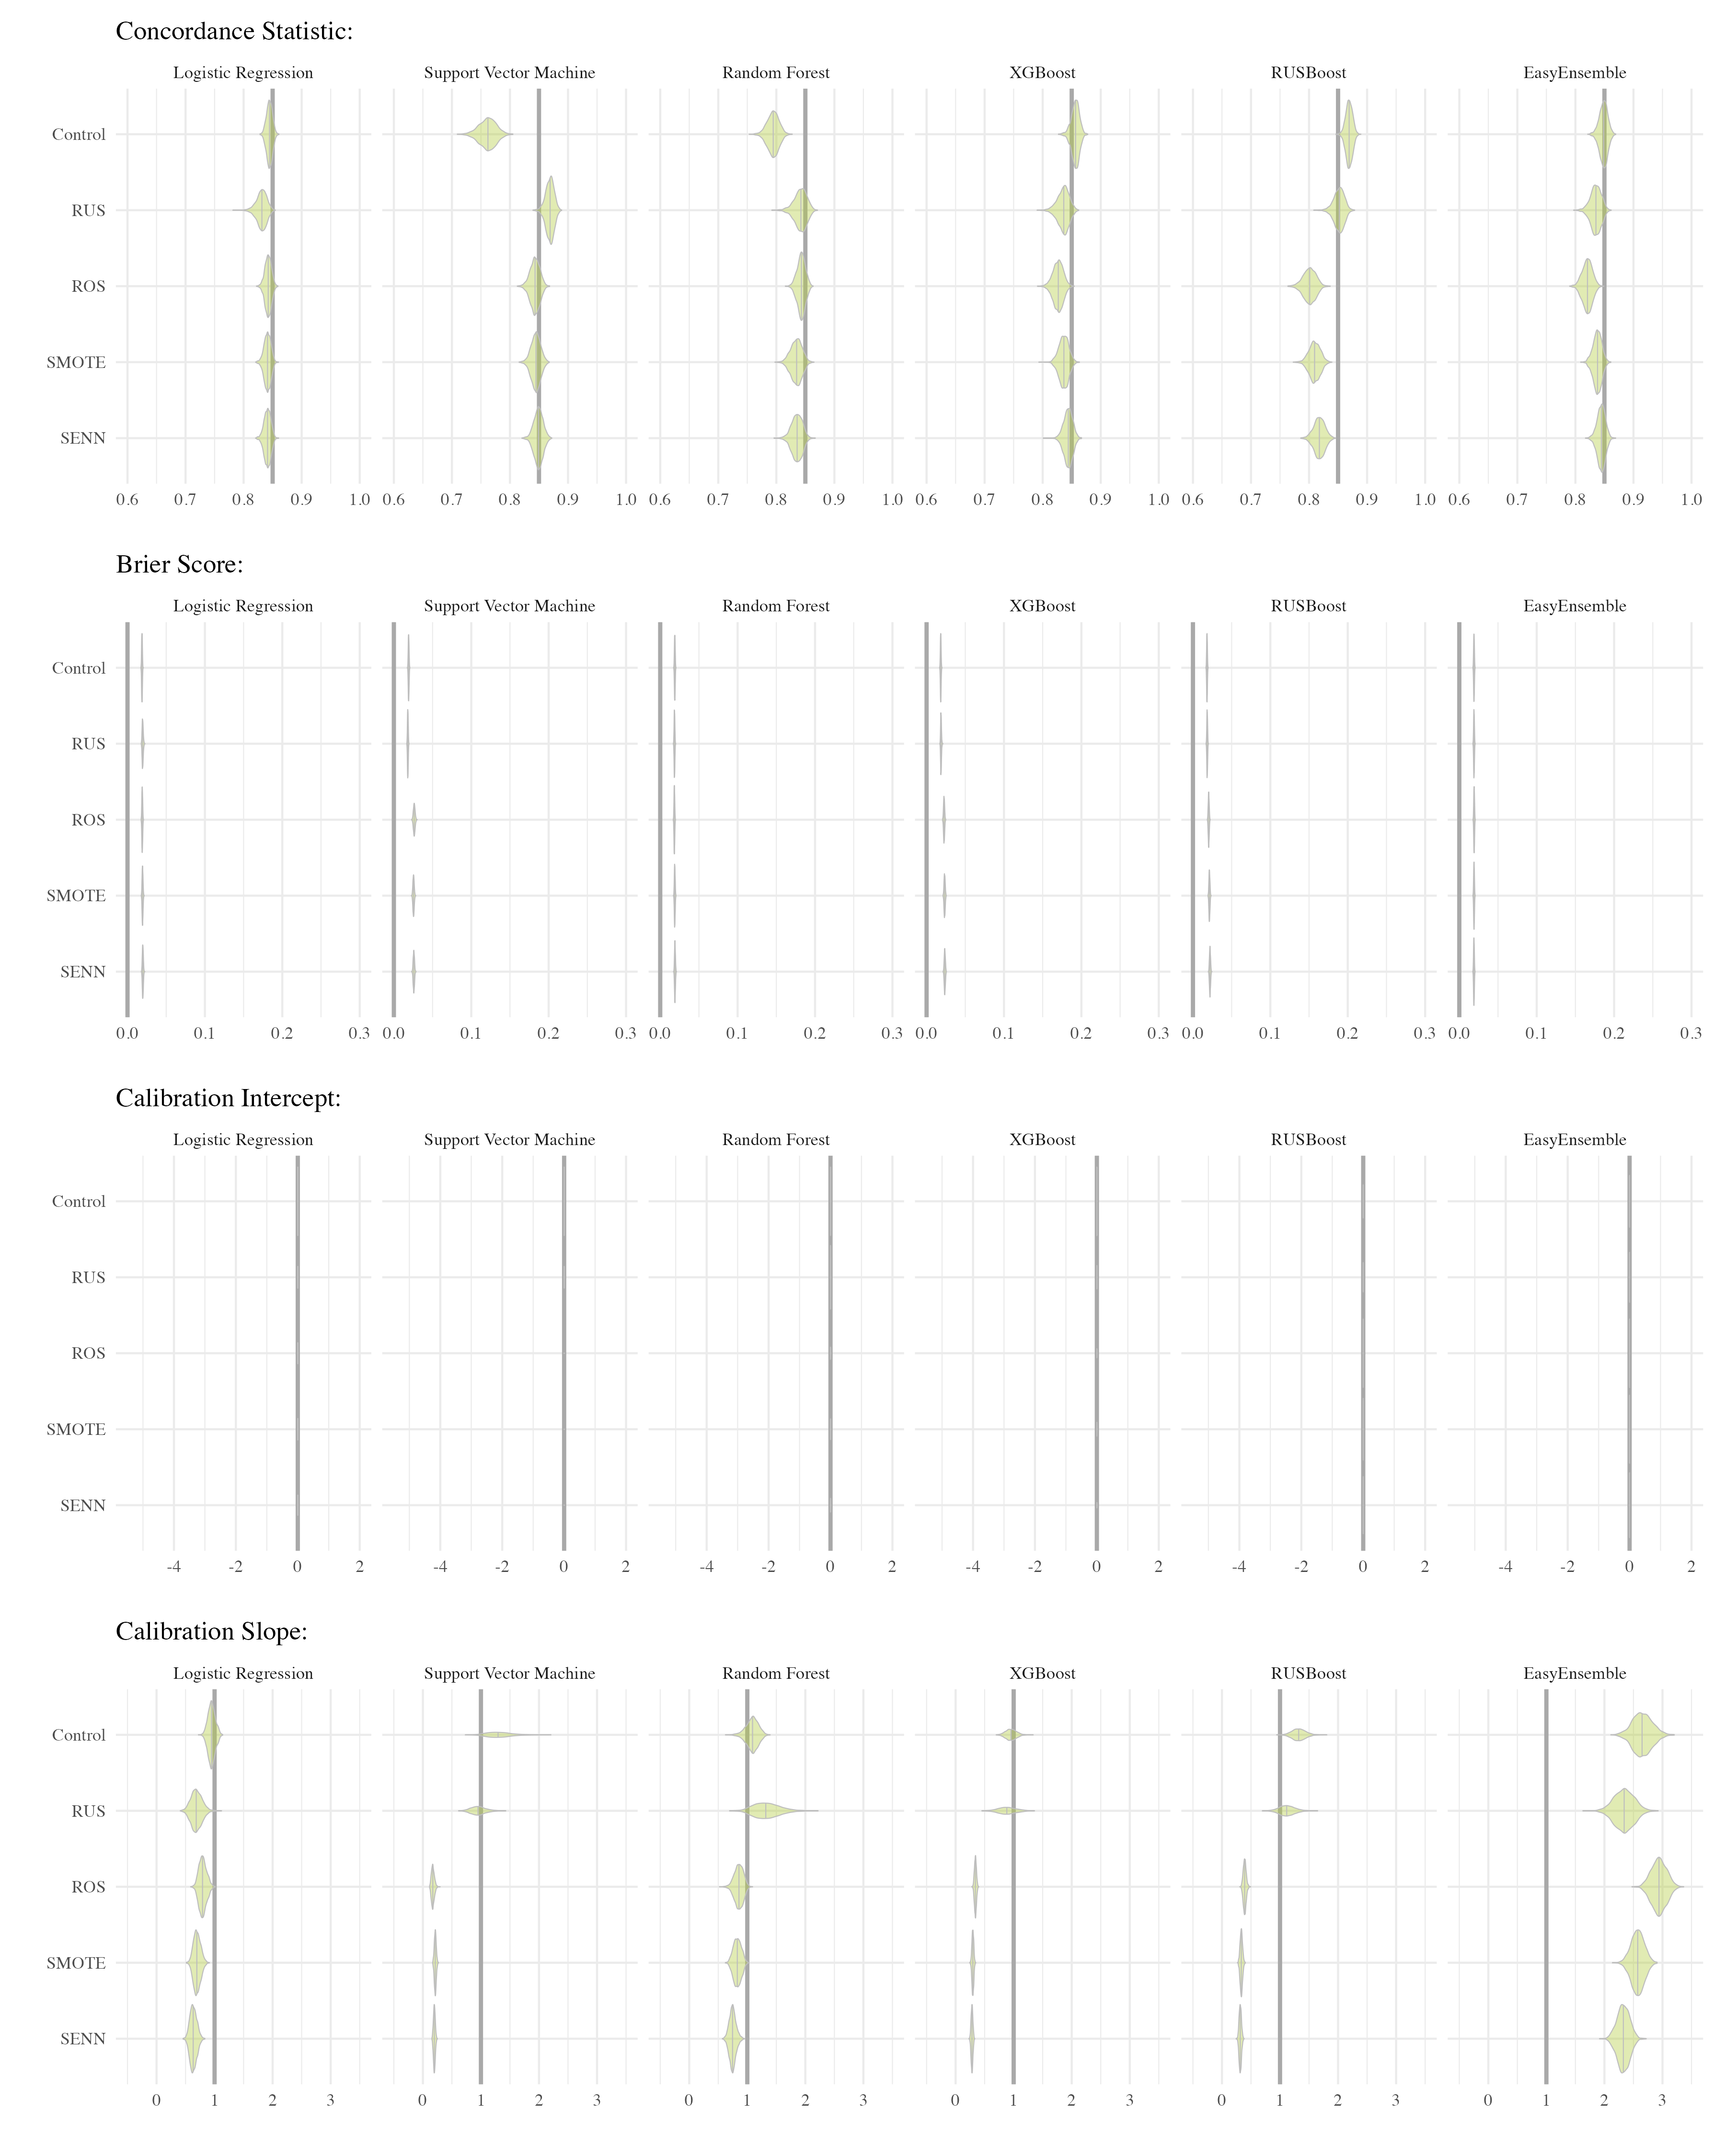
\includegraphics[width=0.7\linewidth]{./figures/performance_metrics_manuscript_sc18_recalibrated} 

}

\caption{Empirical performance metrics for each of 2000 simulation iterations in simulation scenario 18.  This simulation scenario is characterized by 16 predictors, double the required sample size (2N) and strongly imbalanced data (event fraction = 0.02). Empirical performance metrics were computed with re-calibrated predicted risks. The target value highlighted for the concordance statistic reflects the data-generating concordance statstic, 0.85. Imbalance corrections: RUS (random undersampling), ROS (random oversampling), SMOTE (synthetic majority oversampling), SENN (synthetic majority oversampling with Wilson's Edited Nearest Neighbors). Note: after re-calibration, calibration intercepts were essentially zero for every iteration and are therefore not visible on the plot. \label{fig:recal_violin_18}}\label{fig:unnamed-chunk-74}
\end{figure}

\end{document}
